\documentclass[main.tex]{subfiles}


%\externalcitedocument{bibfile}
\begin{document}

\section{Methods}
\subsection{Snowstorm}
While some sources of systematic uncertainty can be easily addressed through re-weighting, such as uncertainties on cosmic ray fluxes, others can have non-trivial effects on the reconstruction of events. 
These `low-level' sources of systematic uncertainty typically, and historically, required a dedicated MC sample where the parameter was perturbed by some fixed, discrete, amount. 
This method becomes intractable when multiple, highly correlated, sources of systematic uncertainty are present. 
To address this, a new method for efficiently determining the effects of these parameters was developed, and is discussed at-length in Reference~\cite{Aartsen_2019_snow}.
%This is called the \textit{Snowstorm}\footenote{The technique formerly known as \textit{MultiSim} method.

Snowstorm relies on two underlying assumptions
\begin{itemize}
    \item The effects of systematic uncertainty are small enough that that they can be treated perturbatively 
    \item MC statistical error is small compared to the data
\end{itemize}
In this context, one can sum over a Monte Carlo ensemble with correlating to a different set of nuisance parameters $\vec{\eta}$, which are distributed according to a prior function $P(\vec{\eta})$.
We also require that this prior function is normalized and symmetric for each nuisance parameter $\eta_{i}$, such that 
\begin{align}
    P(\eta_{i}, \vec{\eta}_{j\neq i}) &= P(-\eta_{i},\vec{\eta}_{j\neq i}) & &\forall i\\
    \int d^{N}\eta P(\vec{\eta}) &= 1
\end{align}
We explicitly choose a prior function for the nuisance parameters that is a product of equal-width Gaussian functions:
\begin{equation}
    P(\vec{\eta}) = \prod_{i} \dfrac{1}{\sigma \sqrt{2\pi}} e^{-\eta_{i}^{2}/2\sigma^{2}}.
\end{equation}

WRITE more

Two Monte Carlo samples were generated to evaluate the effects of various sources of systematic uncertainty on analysis space. 
In one, a sample was generated while allowing the amplitudes and phases, for a Fourier series describing the depth-dependence of the absorption length and scattering length, to vary amounts shown in Table TABLE. 
This is described in detail in Subsection~\ref{sec:bulk}.
In the other sample the DOM efficiency, both unified hole ice parameters were allowed to vary, a parameter effecting ice anisotropy, and two parameters effecting bulk absorption and scattering lengths were allowed to vary. The anisotropy, bulk absorption, and bulk scattering gradients were not used in this analysis. 
Priors used in this sample are shown in Table~\ref{table:snowstorm2}. 

\begin{table}
    \centering
    \rowcolors{2}{gray!25}{white}
    \begin{tabular}{c | ccc}\rowcolor{blue!25}
        Systematic & Sampling Distribution & Range & Comments \\\hline
        Scattering & uniform & [0.9,1.1] & bulk effect, not used\\
        Absorption & uniform & [0.9,1.1] & bulk effect, not used\\
        Anisotropy Scale & uniform & [0,2] & equal to 0-15\%, not used \\
        DOM Efficiency & uniform & [0.9, 1.1] & values shifted down by 0.27 \\
        Unified HoleIce & uniform & \shortstack{p0 $\in$ [-0.84, 0.3] \\ p1 $\in$ [-0.134, 0.05]} & 
    \end{tabular}
    \caption{A table listing all SnowStorm systematic perturbations and their ranges used in the nuisance parameter MC set.}\label{table:snowstorm2}
\end{table}

\subsection{Systematic Downsizing}\label{sect:down}

In this analysis, several sets of nuisance parameters are correlated to various degrees: the astrophysical flux, the cosmic ray flux model and hadronic model, and the absorption and scattering lengths as functions of depth in IceCube. 
A new method for (1) fitting these correlated priors in an uncorrelated way and (2) representing the effects with fewer parameters was developed and adopted. 

Considering a set of $n$ nuisance parameters $\vec{x}$, each with mean $\mu$.
An $n\times n$ matrix, $\Sigma$ defines the positive-definite covariance between these nuisance parameters. 
If we assume the distribution is jointly normally distributed, then the probability density function defining the odds of a set of nuisance parameters $\vec{y}$ being the ``true'' values is given by
\begin{equation}
    P(\vec{y}) = \dfrac{1}{(2\pi)^{n/2}\left|\Sigma\right|^{1/2}}\exp\left[-\tfrac{1}{2}(\vec{y}-\vec{\mu})^{T}\Sigma^{-1}\left(\vec{y}-\vec{\mu}\right)\right]
\end{equation}
where $\left|\Sigma\right|$ is the determinant of the covariance matrix $\Sigma$. 
We then consider the simple coordinate transformation $ \vec{p}\equiv \vec{y}-\vec{\mu}$.
For consistency with goodness of fits tests and usefulness in minimization applications, we also focus on the log of this likelihood distribution. 
\begin{equation}
\mathcal{L} \equiv \log P = -\tfrac{1}{2}\vec{p}^{T}\Sigma^{-1}\vec{p} + C
\end{equation}
We diagonalize this matrix by considering a transformation $U\in SO(N)$ satisfying $A = U\Sigma^{-1}U^{T}$, where $A$ is diagonal. 
\begin{equation}
    \mathcal{L} \equiv \log P = -\tfrac{1}{2}\vec{p}^{T} U^{T} U\Sigma^{-1} U^{T} U\vec{p}
\end{equation}
or where the primed coordinates are the transformed coordinates,
\begin{equation}
    \mathcal{L} \equiv \log P = -\tfrac{1}{2}(\vec{p}')^{T} A \vec{p}'.
\end{equation}
Thus, we can always rotate a correlated nuisance parameter basis to one where the priors on the parameters are uncorrelated. 

To solve for the transformation, all we really have to do is move some terms around starting from the construction of $A$ and $U$, 
\begin{equation} 
    \Sigma U =  U\left[ \begin{array}{cccc}\lambda_{!} & 0 & \ldots & 0 \\
        0 & \lambda_{2} & \ldots & 0 \\
        \vdots & \vdots & \ddots & \vdots \\
        0 & 0 & \ldots & \lambda_{n} \end{array}\right].
\end{equation}
By re-writing the transformation matrix $U$ as a vector of its column vectors $\eta_{i}$, $U=\left[\begin{array}{ccc}\eta_{1} & \ldots & \eta_{n} \end{array}\right]$, then the equation can be expressed simply as 
\begin{equation}
    \Sigma \eta_{i} = \lambda_{i}\eta_{i}.
\end{equation}
The column vectors of the transformation matrix are the right eigenvectors of the covariance matrix, and each of the corresponding eigenvalues of the covariance matrix are the diagonals of the new matrix $A$, and are the squares of the widths of the distribution along the axes in the uncorrelated basis. 

We lay out a procedure then for any given covariance matrix
\begin{enumerate}
    \item Solve for its eigenvalues and eigenvectors; the values each represent a normal prior width for new, uncorrelated, parameters in the new basis
    \item The block-matrix of the eigenvectors is the transformation matrix allowing for transforming from the correlated basis to the uncorrelated basis. 
    \item Fits are performed in the uncorrelated basis - to evaluate effects of systematic uncertainty we transform whatever point is in question back to the correlated basis and evaluate the effects using the original parametrization. 
\end{enumerate}

\section{Applications}
\subsection{DOM Efficiency}\label{subsect:domeff}

To evaluate the effects of varying the DOM efficiency on reconstructed event rates, a Monte Carlo sample was generated following the Snowstorm method for low-level systematic uncertainties.

For each batch of ten simulated MC events the DOM efficiency is sampled from its prior. 
The wavelength acceptance of the DOMS in CLSim is then adjusted according to the new DOM model, and the photon propagation is carried out. 
The remainder of the MC simulation chain is then performed.
The final-level MC is then weighted, one at a time, to the conventional, prompt, and astrophysical neutrino fluxes. 

In order to calculate the effects of perturbing the DOM efficiency on the reconstrucion level quantities, we bin events in terms of $\log_{E_{\nu}^{reco}}$, $\cos\theta_{\nu}^{reco}$, and the events' sampled DOM efficiencies. 
We then account for the sampling bias in each DOM efficiency bin by integrating the prior PDF over each DOM efficiency bin and scaling up the weights of events in those bins by one over the cumulative probability of sampling that given bin. 
The sum of the weights in each bin therefore would be a function only of (1) the central expectation in that bin and (2) the bias generated by using a perturbed DOM efficiency. 
For each ($\log E_{\nu}^{reco}$, $\cos\theta_{\nu}^{reco}$) slice, each DOM efficiency bin is then rescaled around the central bin's value; this yields a quantity in each bin that represents the proportional effect of perturbing the DOM efficiency. 

Then, a spline fit is carried out over the full 3D binned space using Photospline~\cite{WHITEHORN20132214}. 
Events can then be reweighted to a new DOM efficiency by evaluating the spline $\mathcal{S}$ at the event's reconstructed energy and zenith, and the new DOM efficiency $\mathcal{D}_{OM}$; this is shown in Equation~EQ.
\begin{equation}\label{eq:domeff}
    w' = w + w\times \mathcal{S}(\log E_{\nu}^{reco}, \cos\theta_{\nu}^{reco}, \mathcal{D}_{OM})
\end{equation}

A slice of the full 3D fit for the conventional neutrino fluxes is shown in Figure~\ref{fig:domeff_fit}.
\begin{figure}
    \centering
    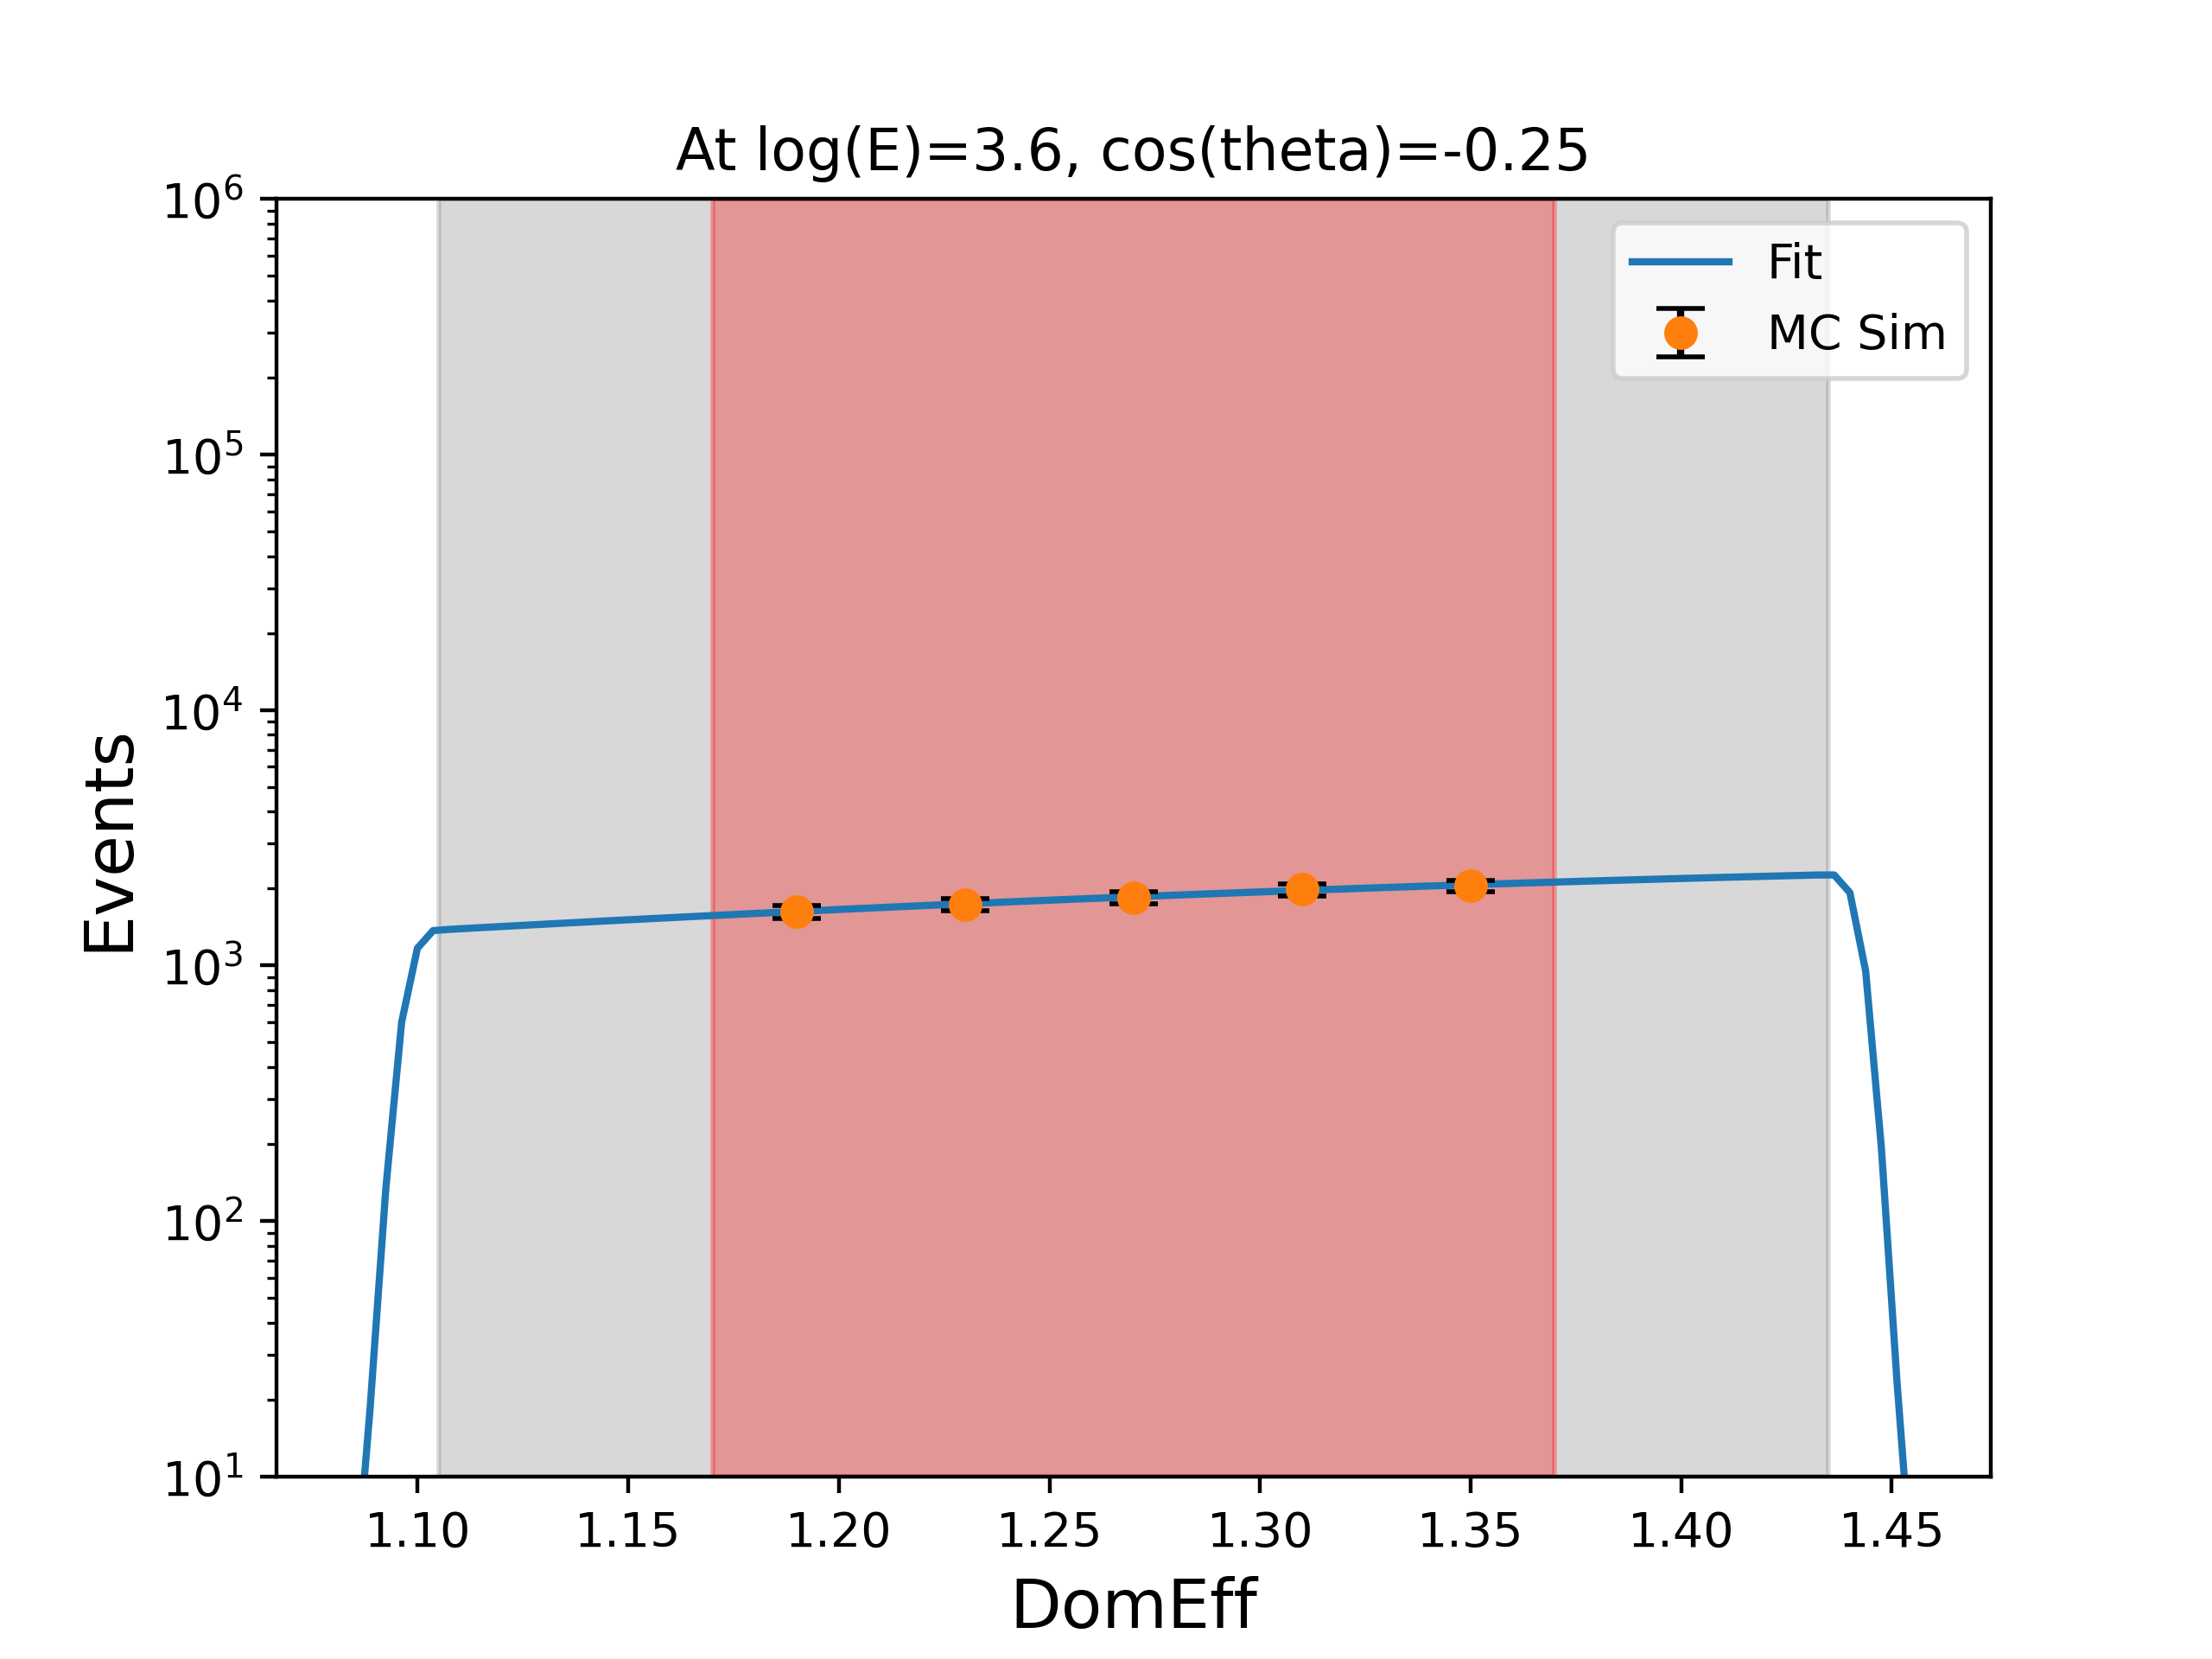
\includegraphics[width=0.8\linewidth]{figures/atmConv_logE_3.6_cosz_-0.25.png}
    \caption{The predicted number of events in reconstructed space for a bin centered at $\log E_{\nu}^{reco}=3.6$ and $\cos\theta_{\nu}^{reco}=0.25$ as a function of the DOM efficiency. The MC data are represented by orange dots, and the spline fit is the trend in blue. The gray shaded region represent the extents of the spline, and the red bands represents prior-allowed region.}\label{fig:domeff_fit}
\end{figure}

The effects on overall reconstructed even rates are shown in Figure~\ref{fig:domeff_analysis} for tracks (left) and cascades (right). 

\begin{figure}
    \centering
    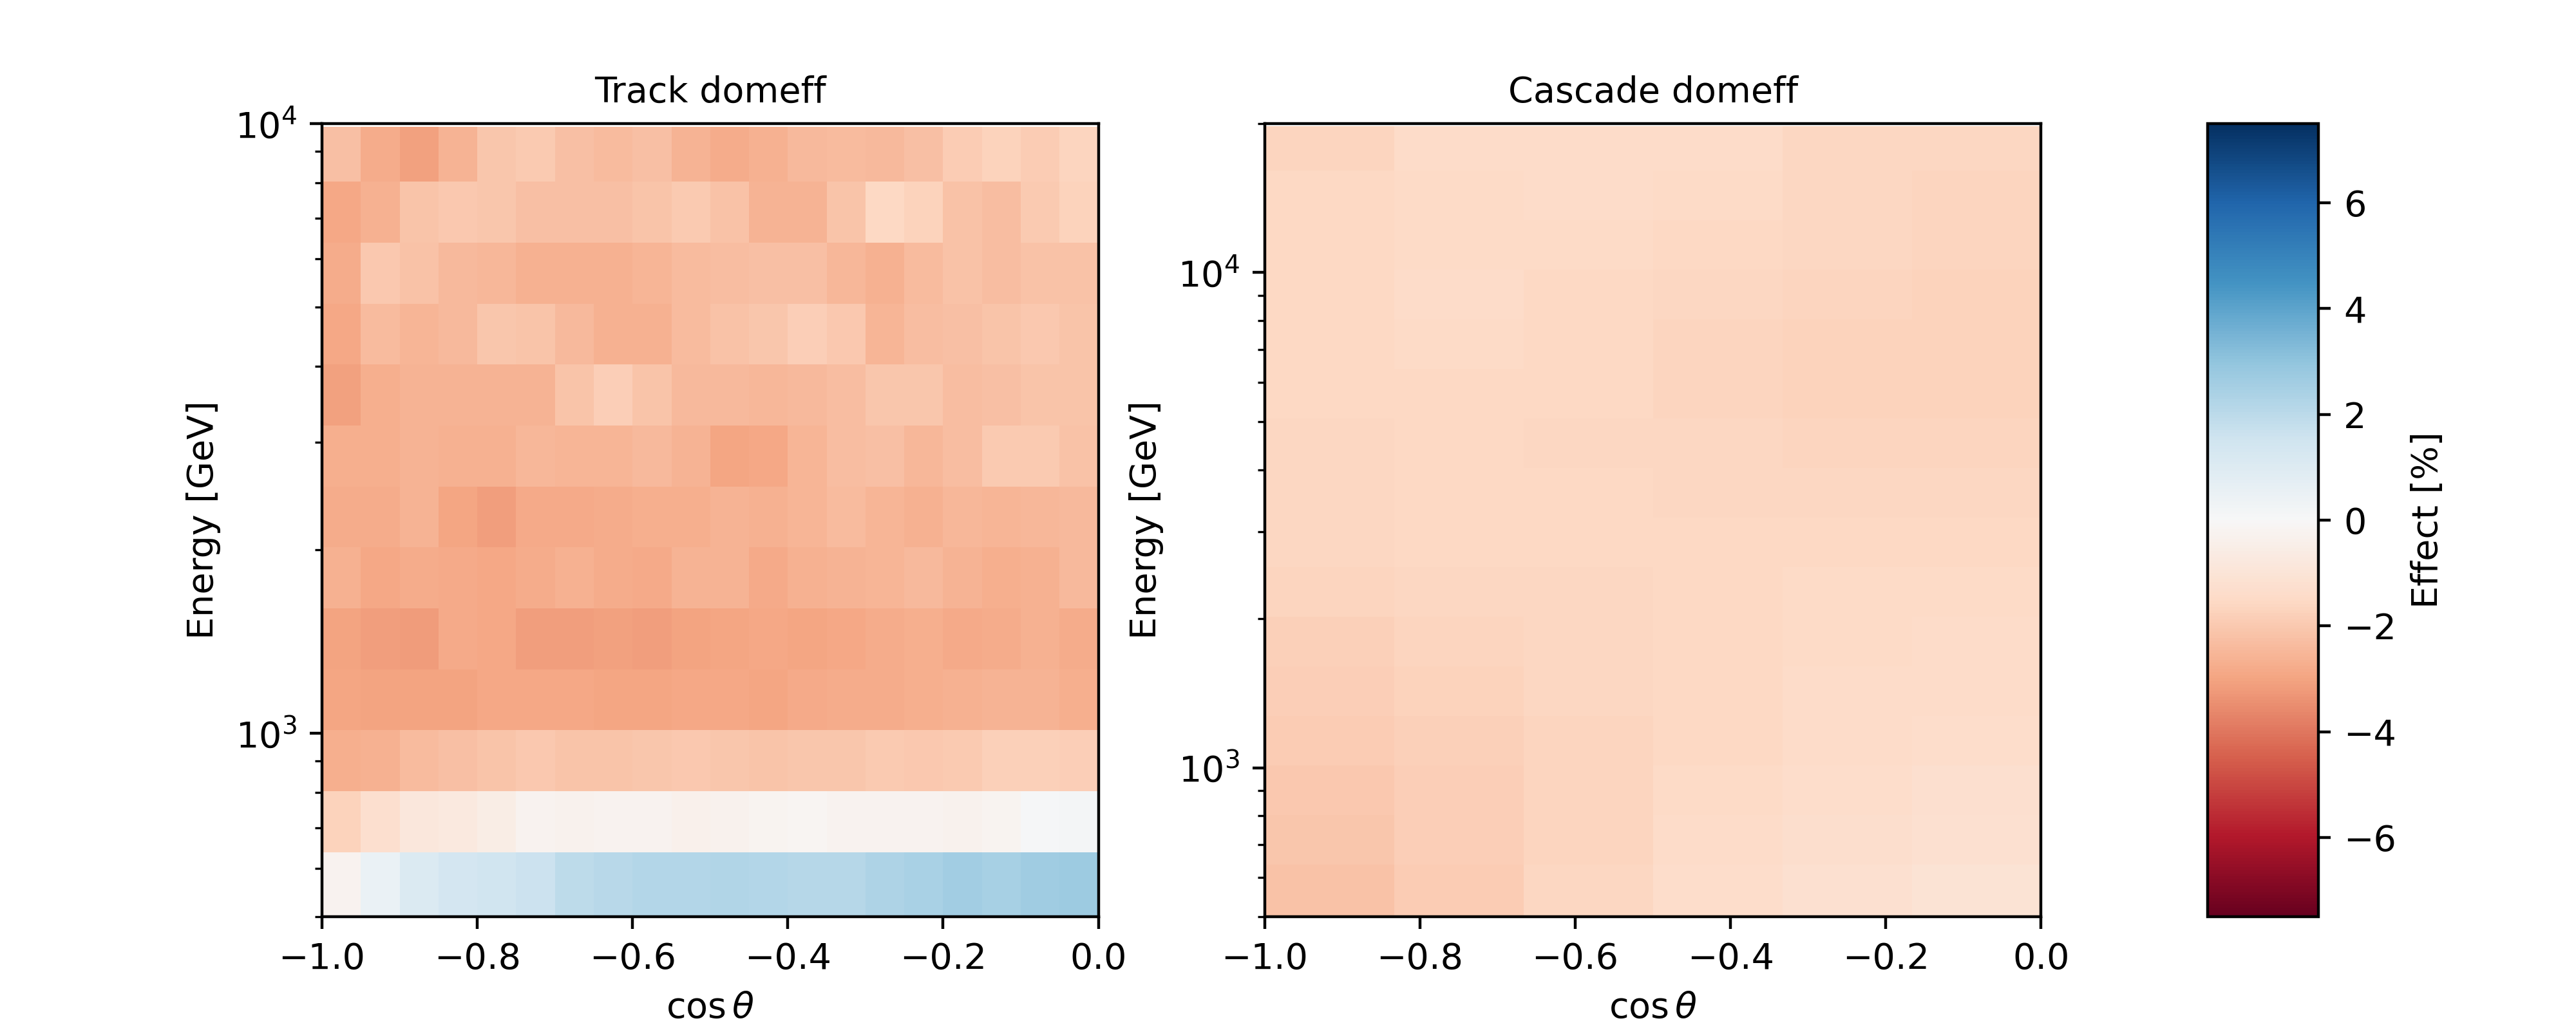
\includegraphics[width=0.8\linewidth]{figures/systematics/domeff.png}
    \caption{The effects of perturbing the DOM efficiency on expected numbers of tracks (left) and cascades (right).}\label{fig:domeff_analysis}
\end{figure}

\subsection{Bulk Ice}\label{sec:bulk}

The bulk ice in the ice is characterised by uncertainties in the absorption and scattering length. 
Initially, every ten meter section of the ice was assigned an absorption length and a scattering length with some uncertainty. 
Over the 1500 meter span of IceCube, this would require 300 separate nuisance parameters to account for these parameters fully.

This is an overwhelming and intractable quantity. 
For this and similar analyses, a Fourier decomposition of the depth ($x$) dependence of the absorption and scattering is used instead, as described in Ref~\cite{Aartsen_2019_snow}: 
\begin{equation}
    \dfrac{1}{2}\log\left(\text{Abs} \times \text{Sca}\right) = \dfrac{A_{0}}{2} +\sum\limits_{n=1}^{N}A_{n} \sin\left(\dfrac{2\pi nx}{L} + \phi_{n}\right)
\end{equation}
where $A_{n}$ and $\phi_{n}$ are amplitudes and phases for the $n$'th term in the series expansion, $L$ is the vertical extent of IceCube, and \textit{Abs} and \textit{Sca} are the in-ice absorption and scattering lengths. 


To calibrate these amplitudes and phases and to determine the covariance between them, we use the IceCube in-situ flasher data~\cite{Aartsen_2013}. 
These use the 12 on-board LEDs mounted in the housings of each DOM. 
The LEDs on all DOMs of string 63 are flashed, and then the measured light throughout IceCube, minus string 63, is logged. 
Then, PPC simulations were carried out for various, perturbed, ice models were performed. 
PPC simulations were performed by perturbing the amplitudes and phases for the first four modes in the Fourier series expansion of the depth dependence of absorption and scattering in the bulk ice.
PPC simulations were also performed by perturbing various combinations of these modes. 
These PPC simulations were used, in conjunction with the measured flasher data, to quantify the likelihood of the observed data assuming different ice models,

For each amplitude and phase, these likelihoods were calculated for icemodels where the first five Fourier amplitudes and the first four Fourier phases were shifted. 
These values were shifted large amounts first, from which an approximate minimum and width was determined. 
Then, more granular PPC simulations were carried out by varying these amplitudes and phases about the approximate centers. 
Off-axis simulations were also carried out by shifting every possible combination of nuisance parameters, either both positively or both negatively, by varying amounts. 


For each amplitude and phase a quadratic fit was then done to the log likelihood distributions, 
\begin{equation}
    \mathcal{L}(\eta_{i}) = A_{i}\eta_{i}^{2} + B_{i}\eta_{i} + C_{i}
\end{equation}
where $\eta_{i}$ is for any one amplitude or phase. These fits are shown in Figure~\ref{fig:linearfit} after being normalized by the minimum likelihood found in each fit, and were carried out to verify that these nuisance parameters are normally distributed about the minima. 
A similar scan was then done for combinations of nuisance parameters by shifting each possible pairing of them by amounts proportional to the widths of the nuisance parameters. 

\begin{figure}
    \centering
    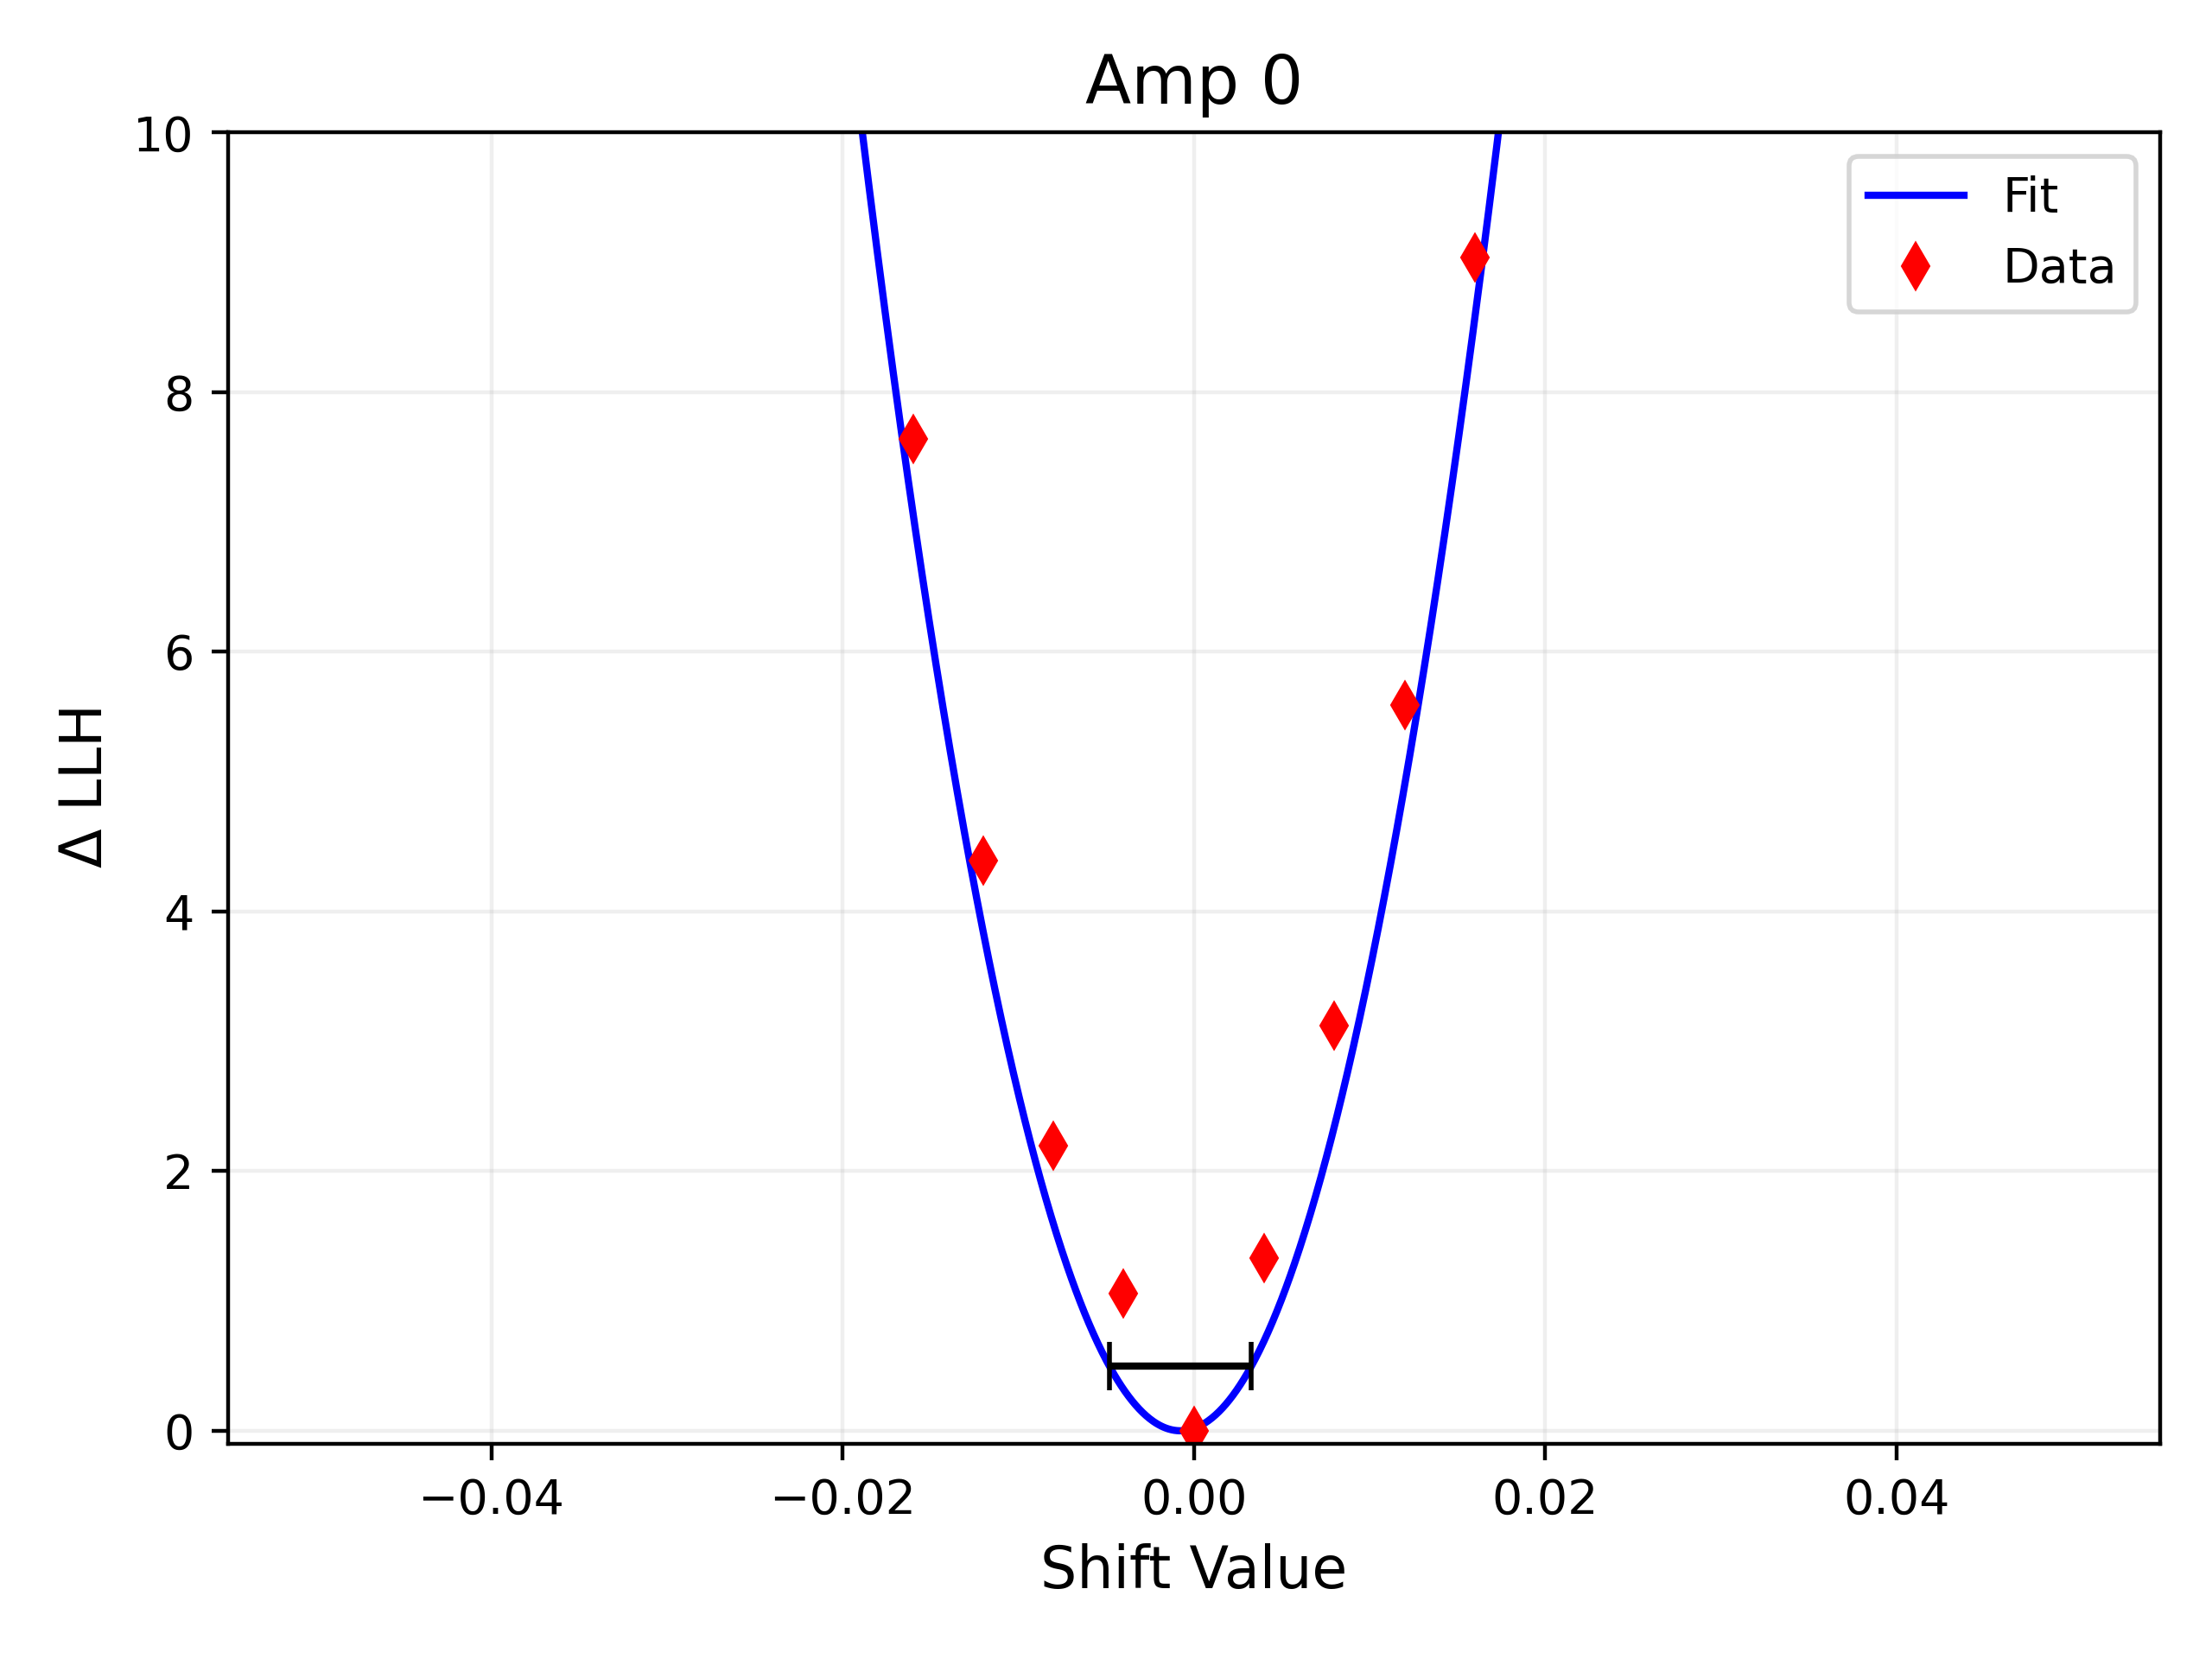
\includegraphics[width=0.3\linewidth]{figures/ice_fits/Amp_0_llhfunc.png}%
    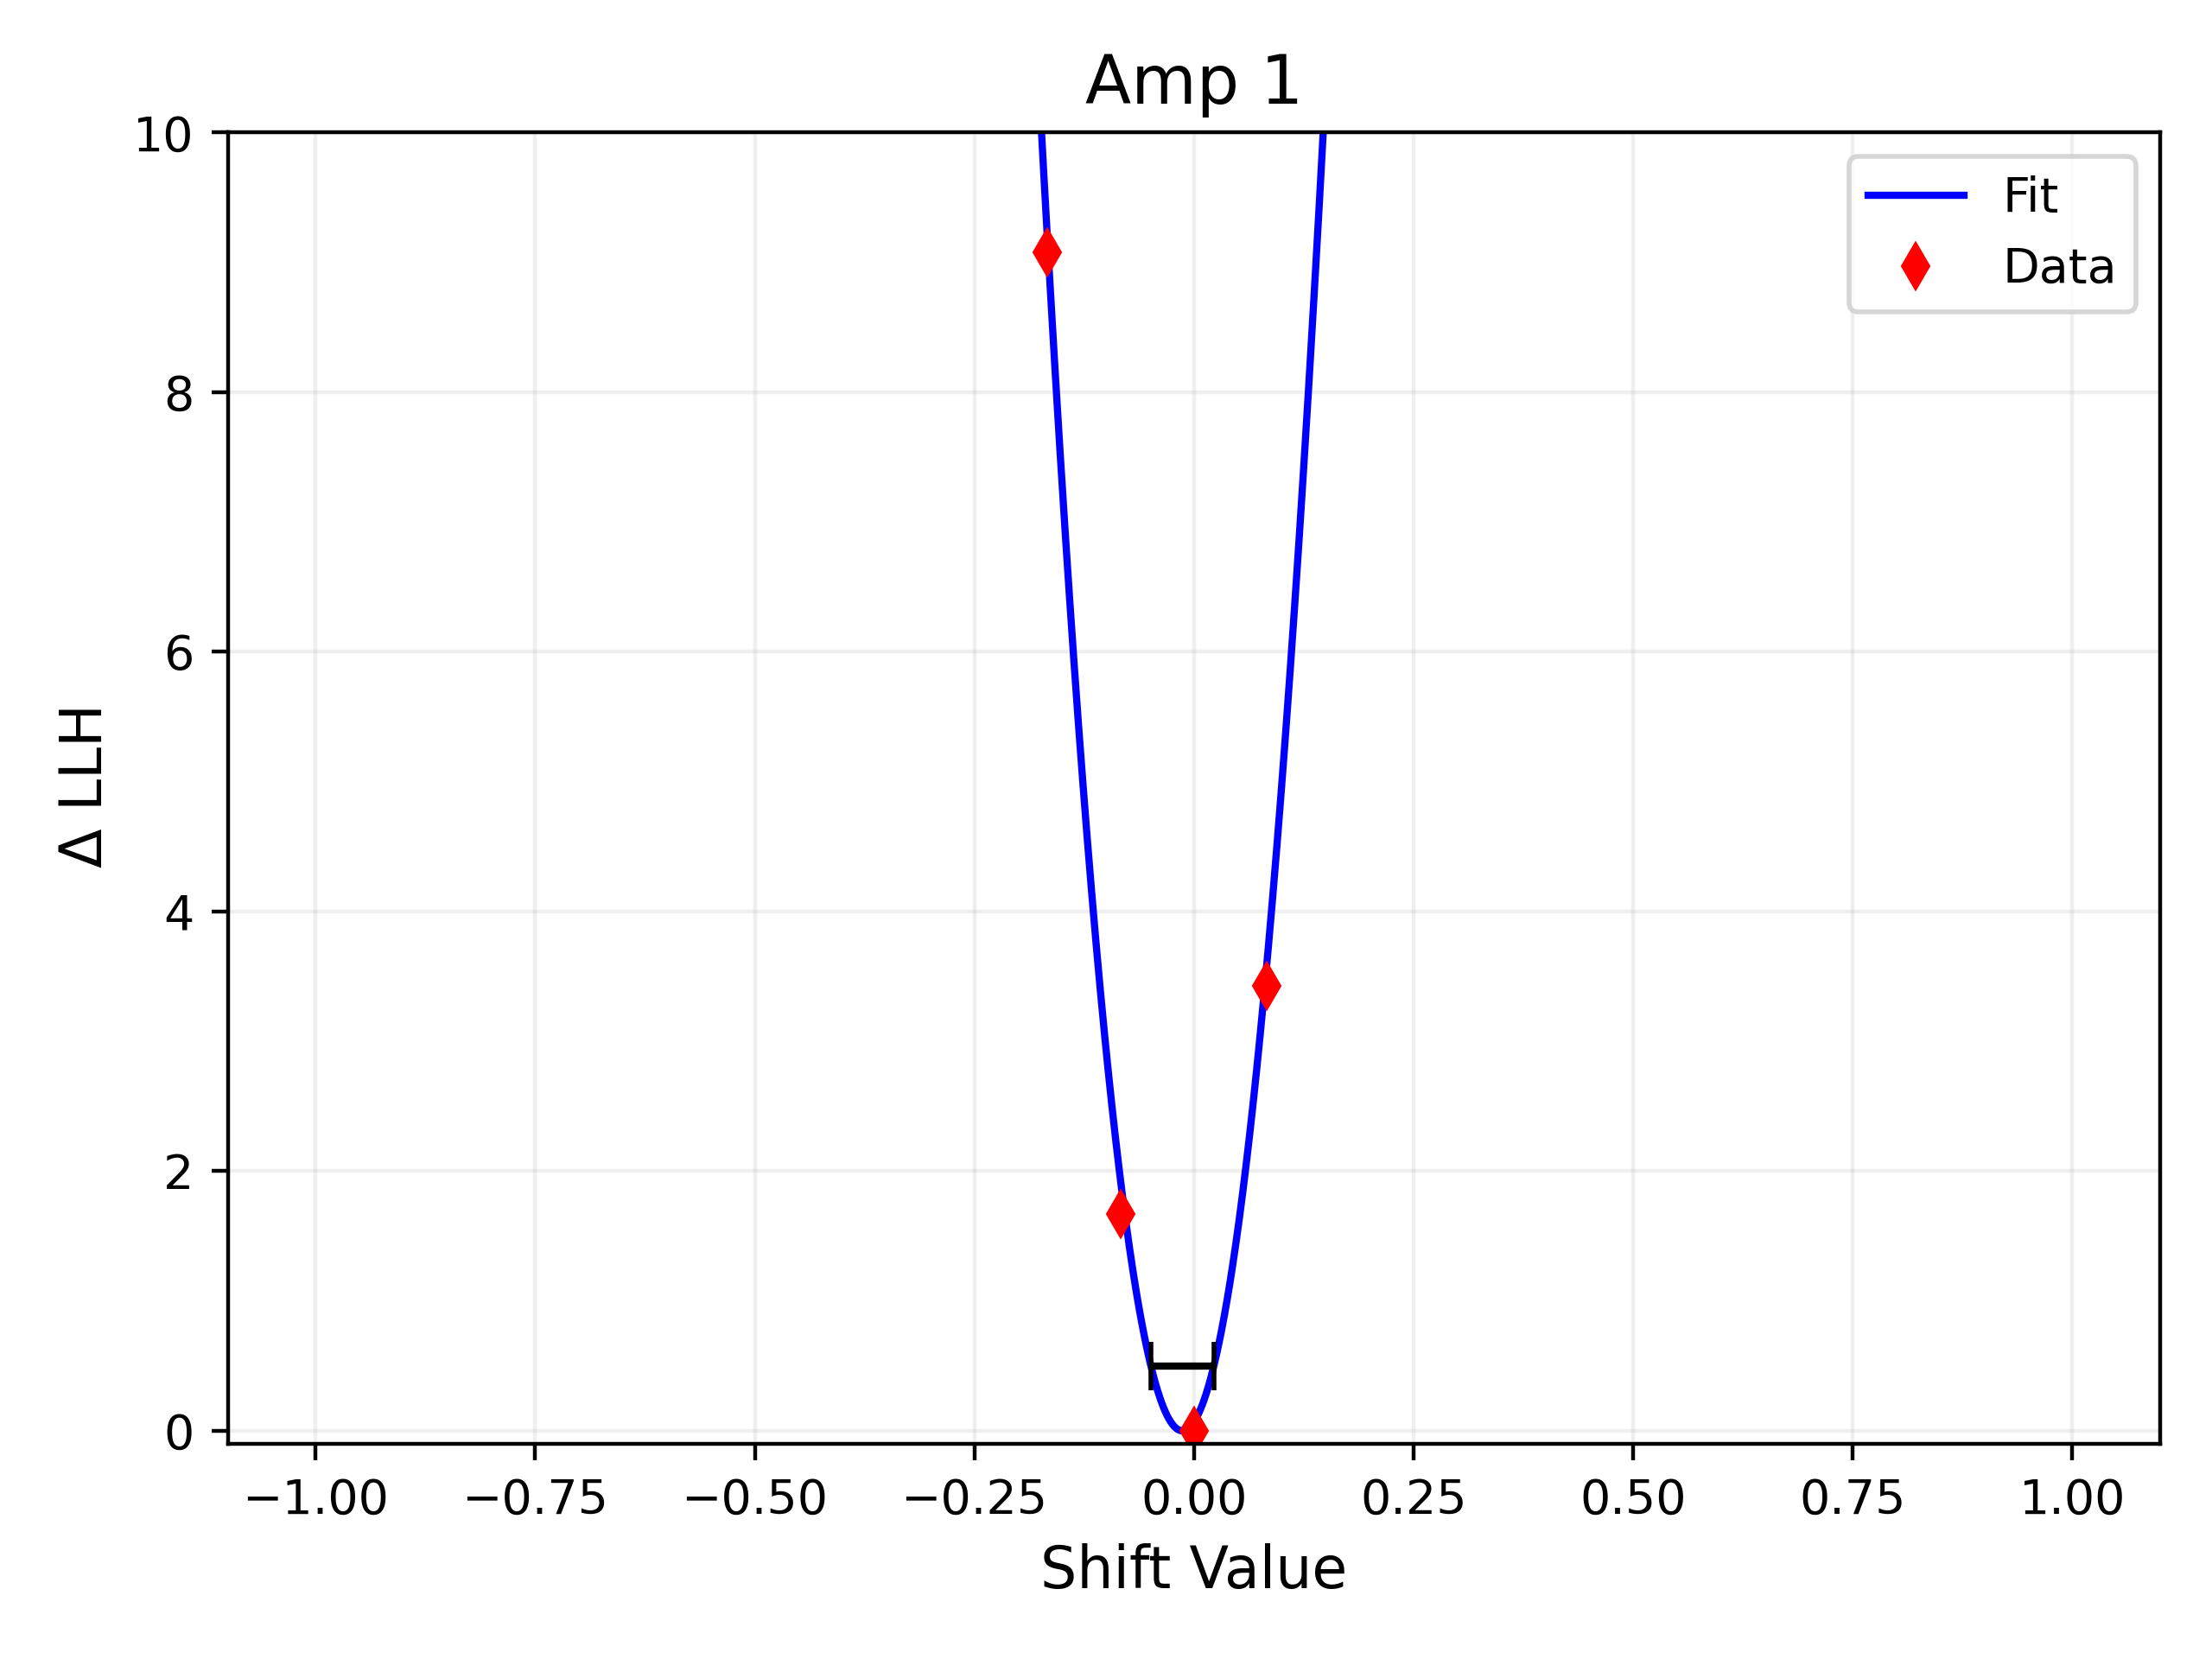
\includegraphics[width=0.3\linewidth]{figures/ice_fits/Amp_1_llhfunc.png}%
    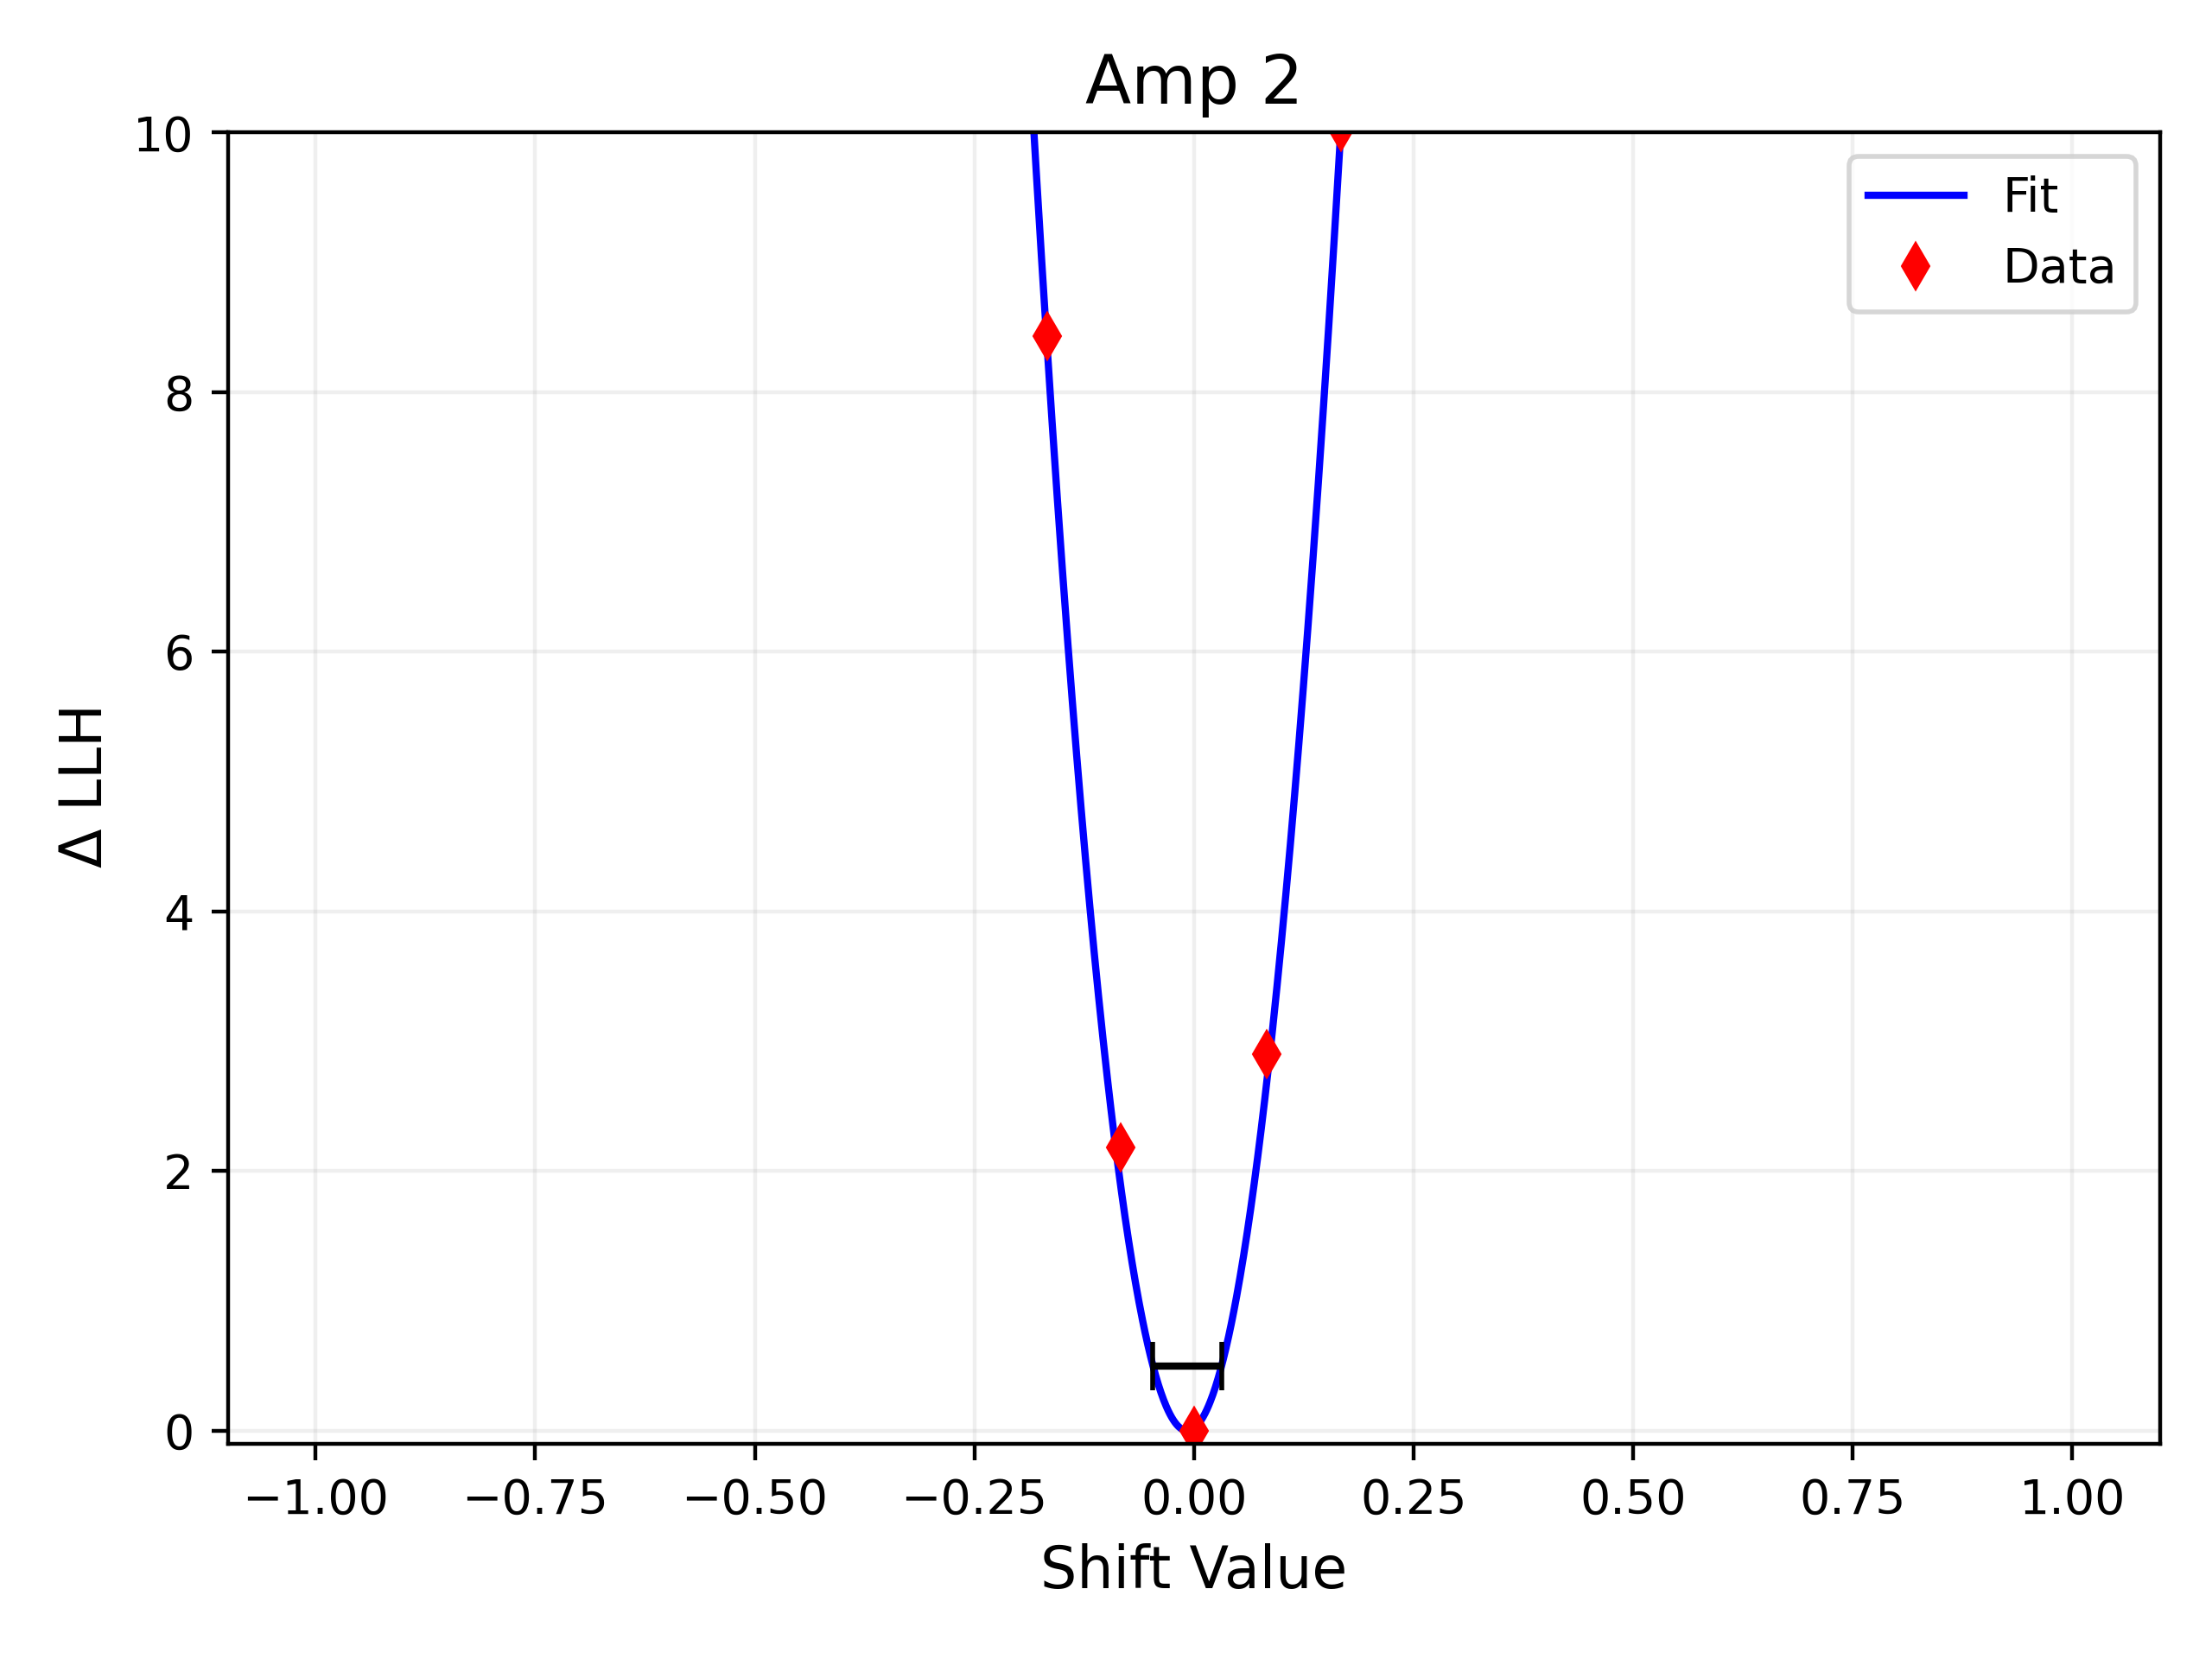
\includegraphics[width=0.3\linewidth]{figures/ice_fits/Amp_2_llhfunc.png}\\
    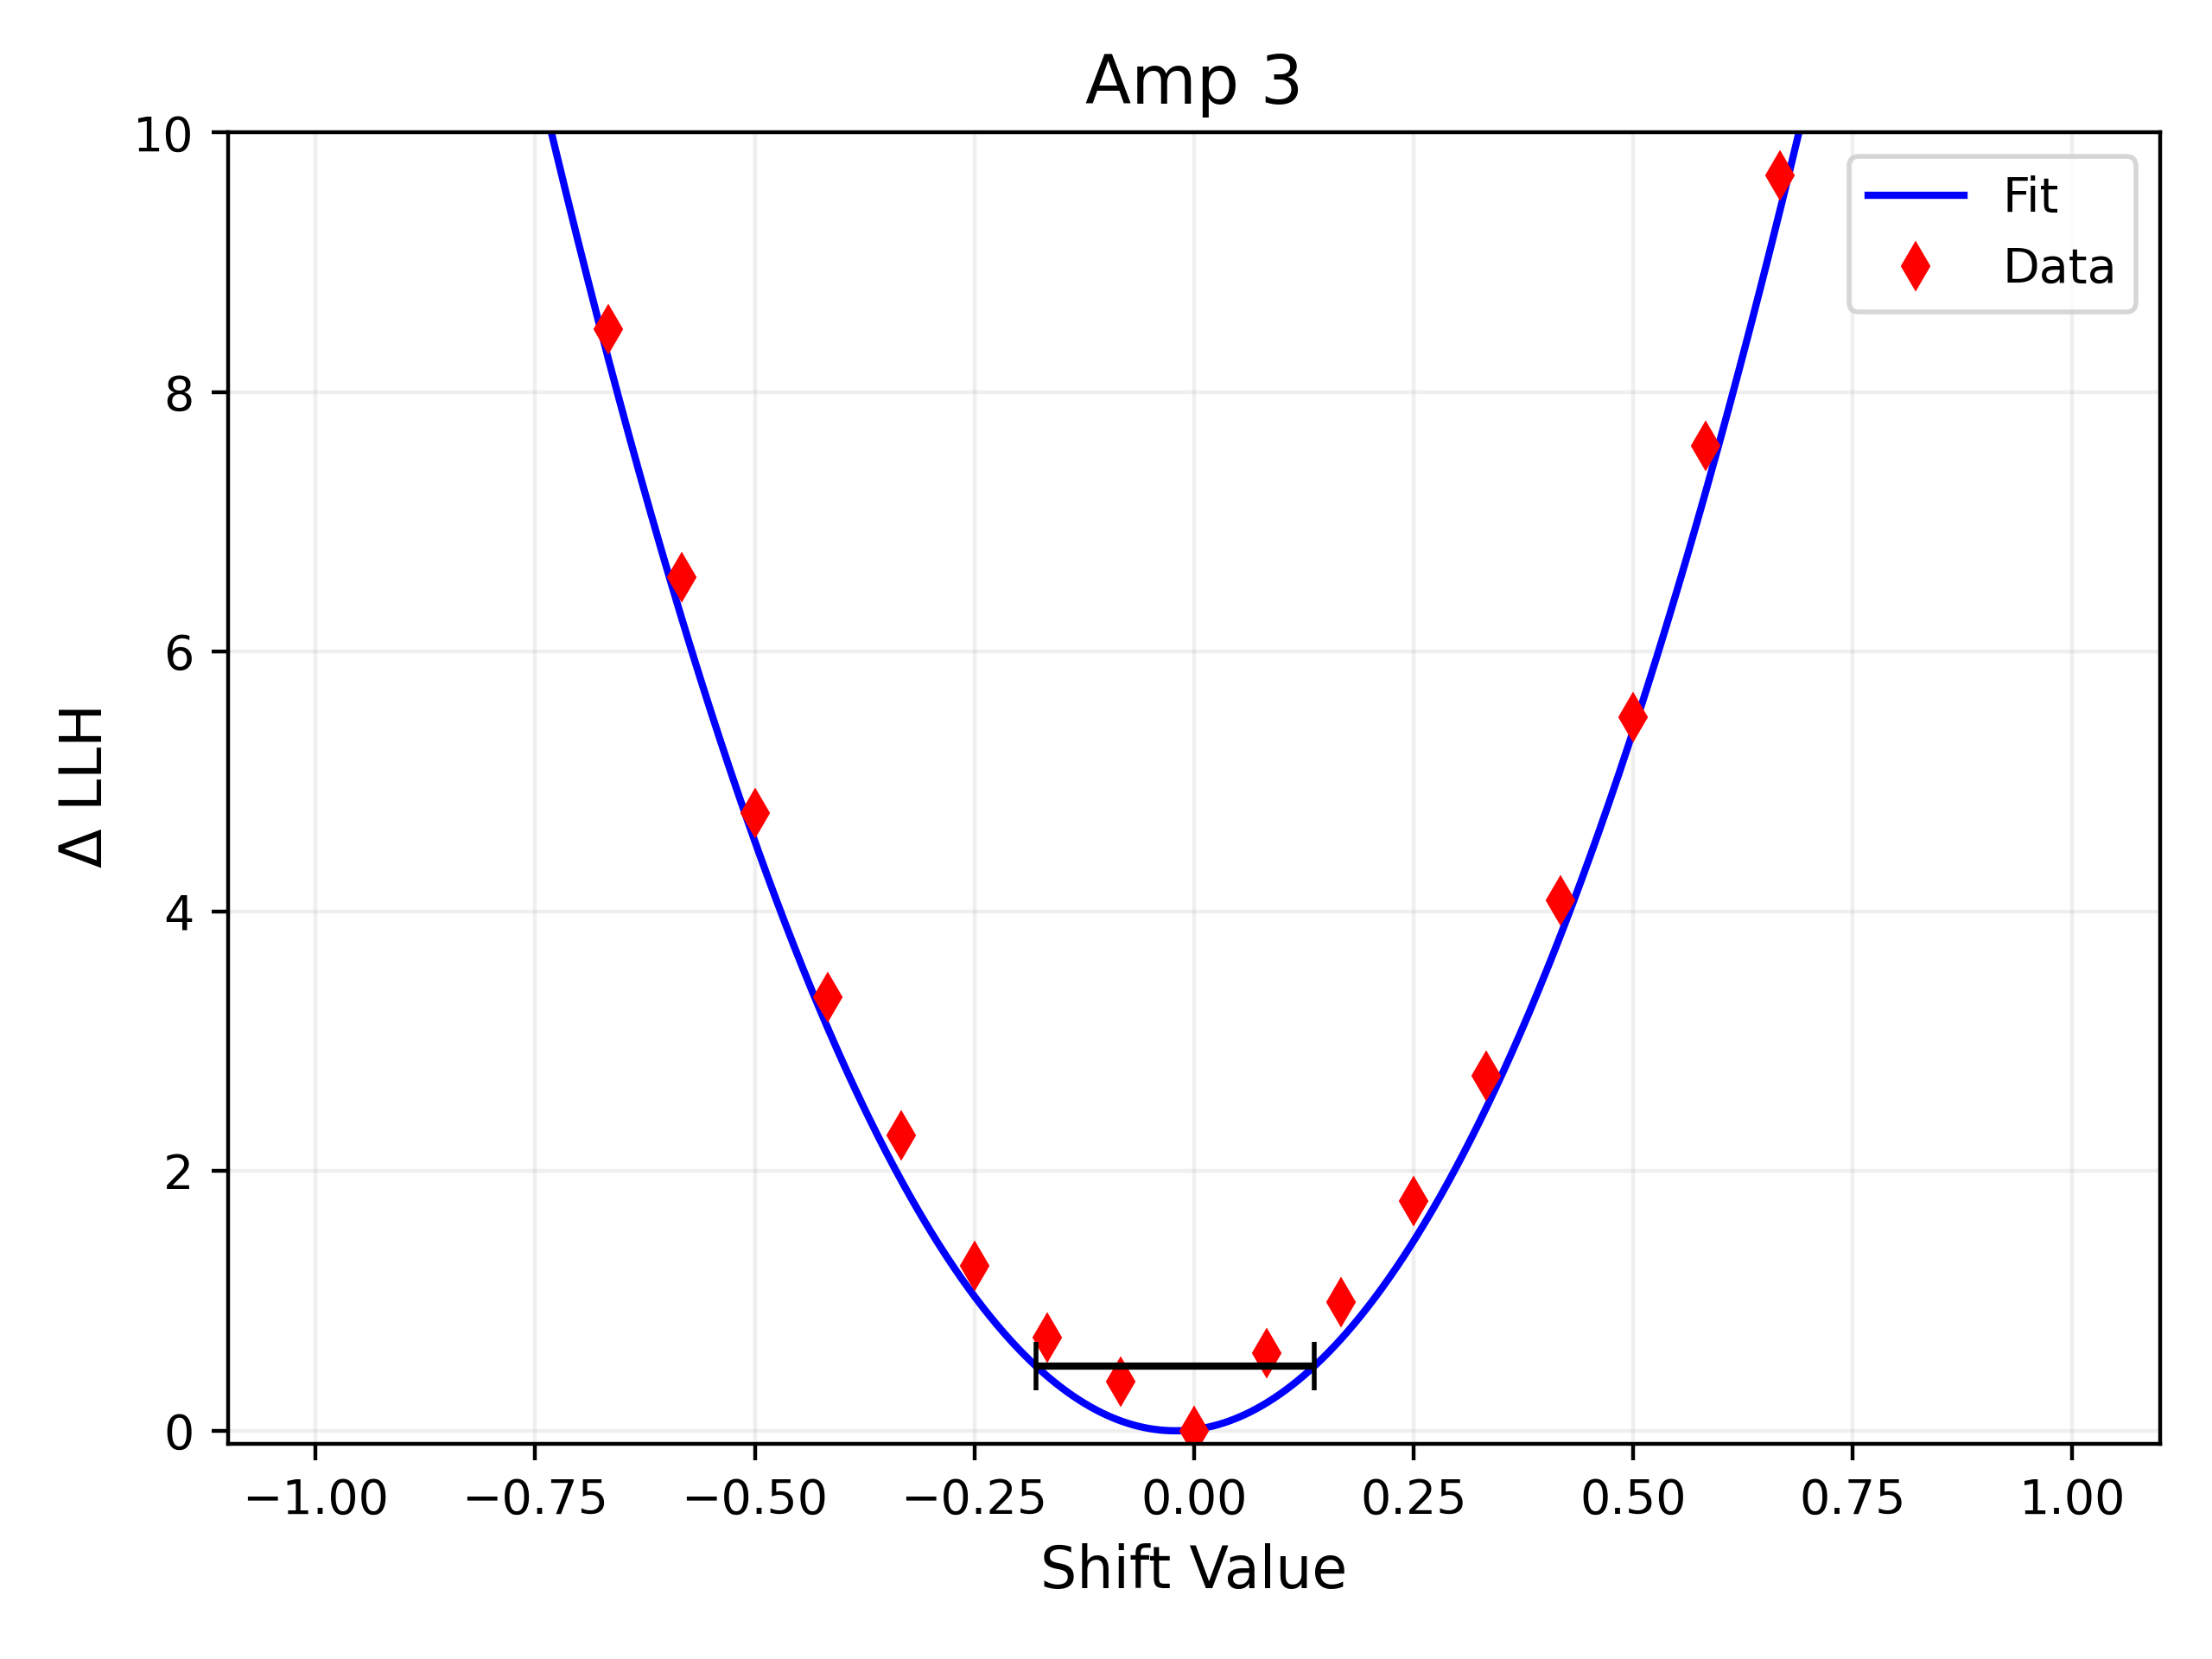
\includegraphics[width=0.3\linewidth]{figures/ice_fits/Amp_3_llhfunc.png}%
    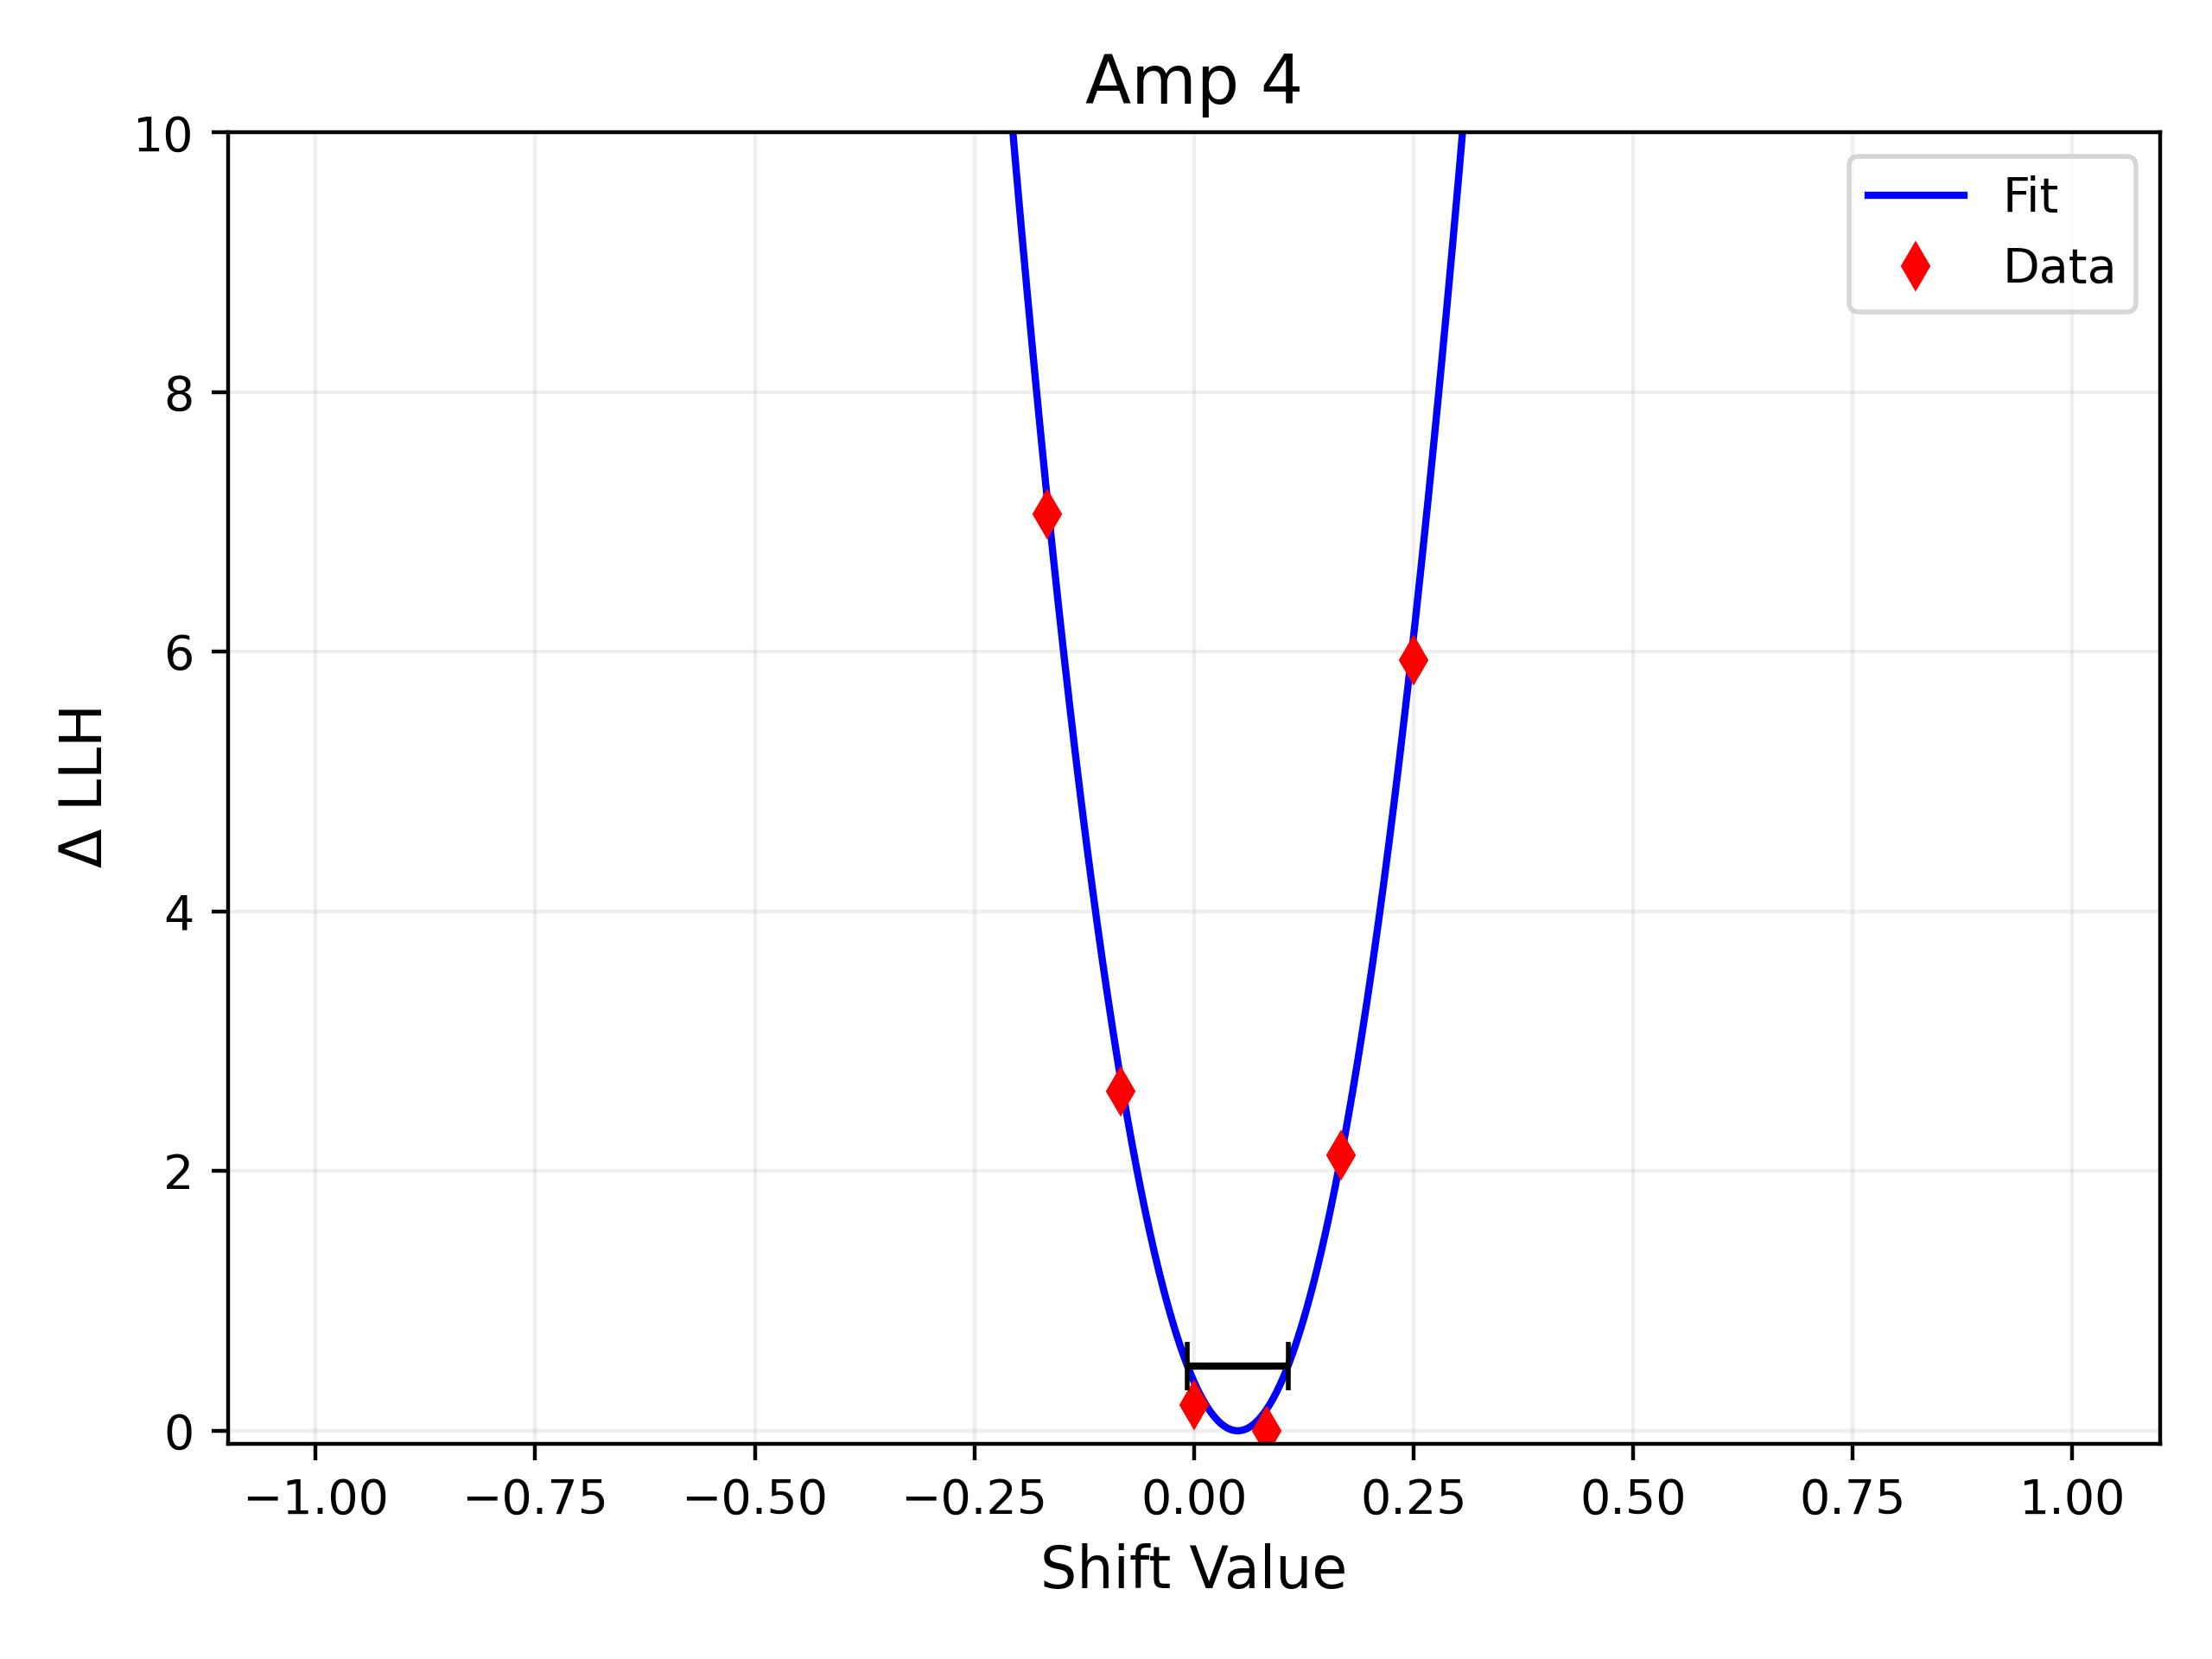
\includegraphics[width=0.3\linewidth]{figures/ice_fits/Amp_4_llhfunc.png}%
    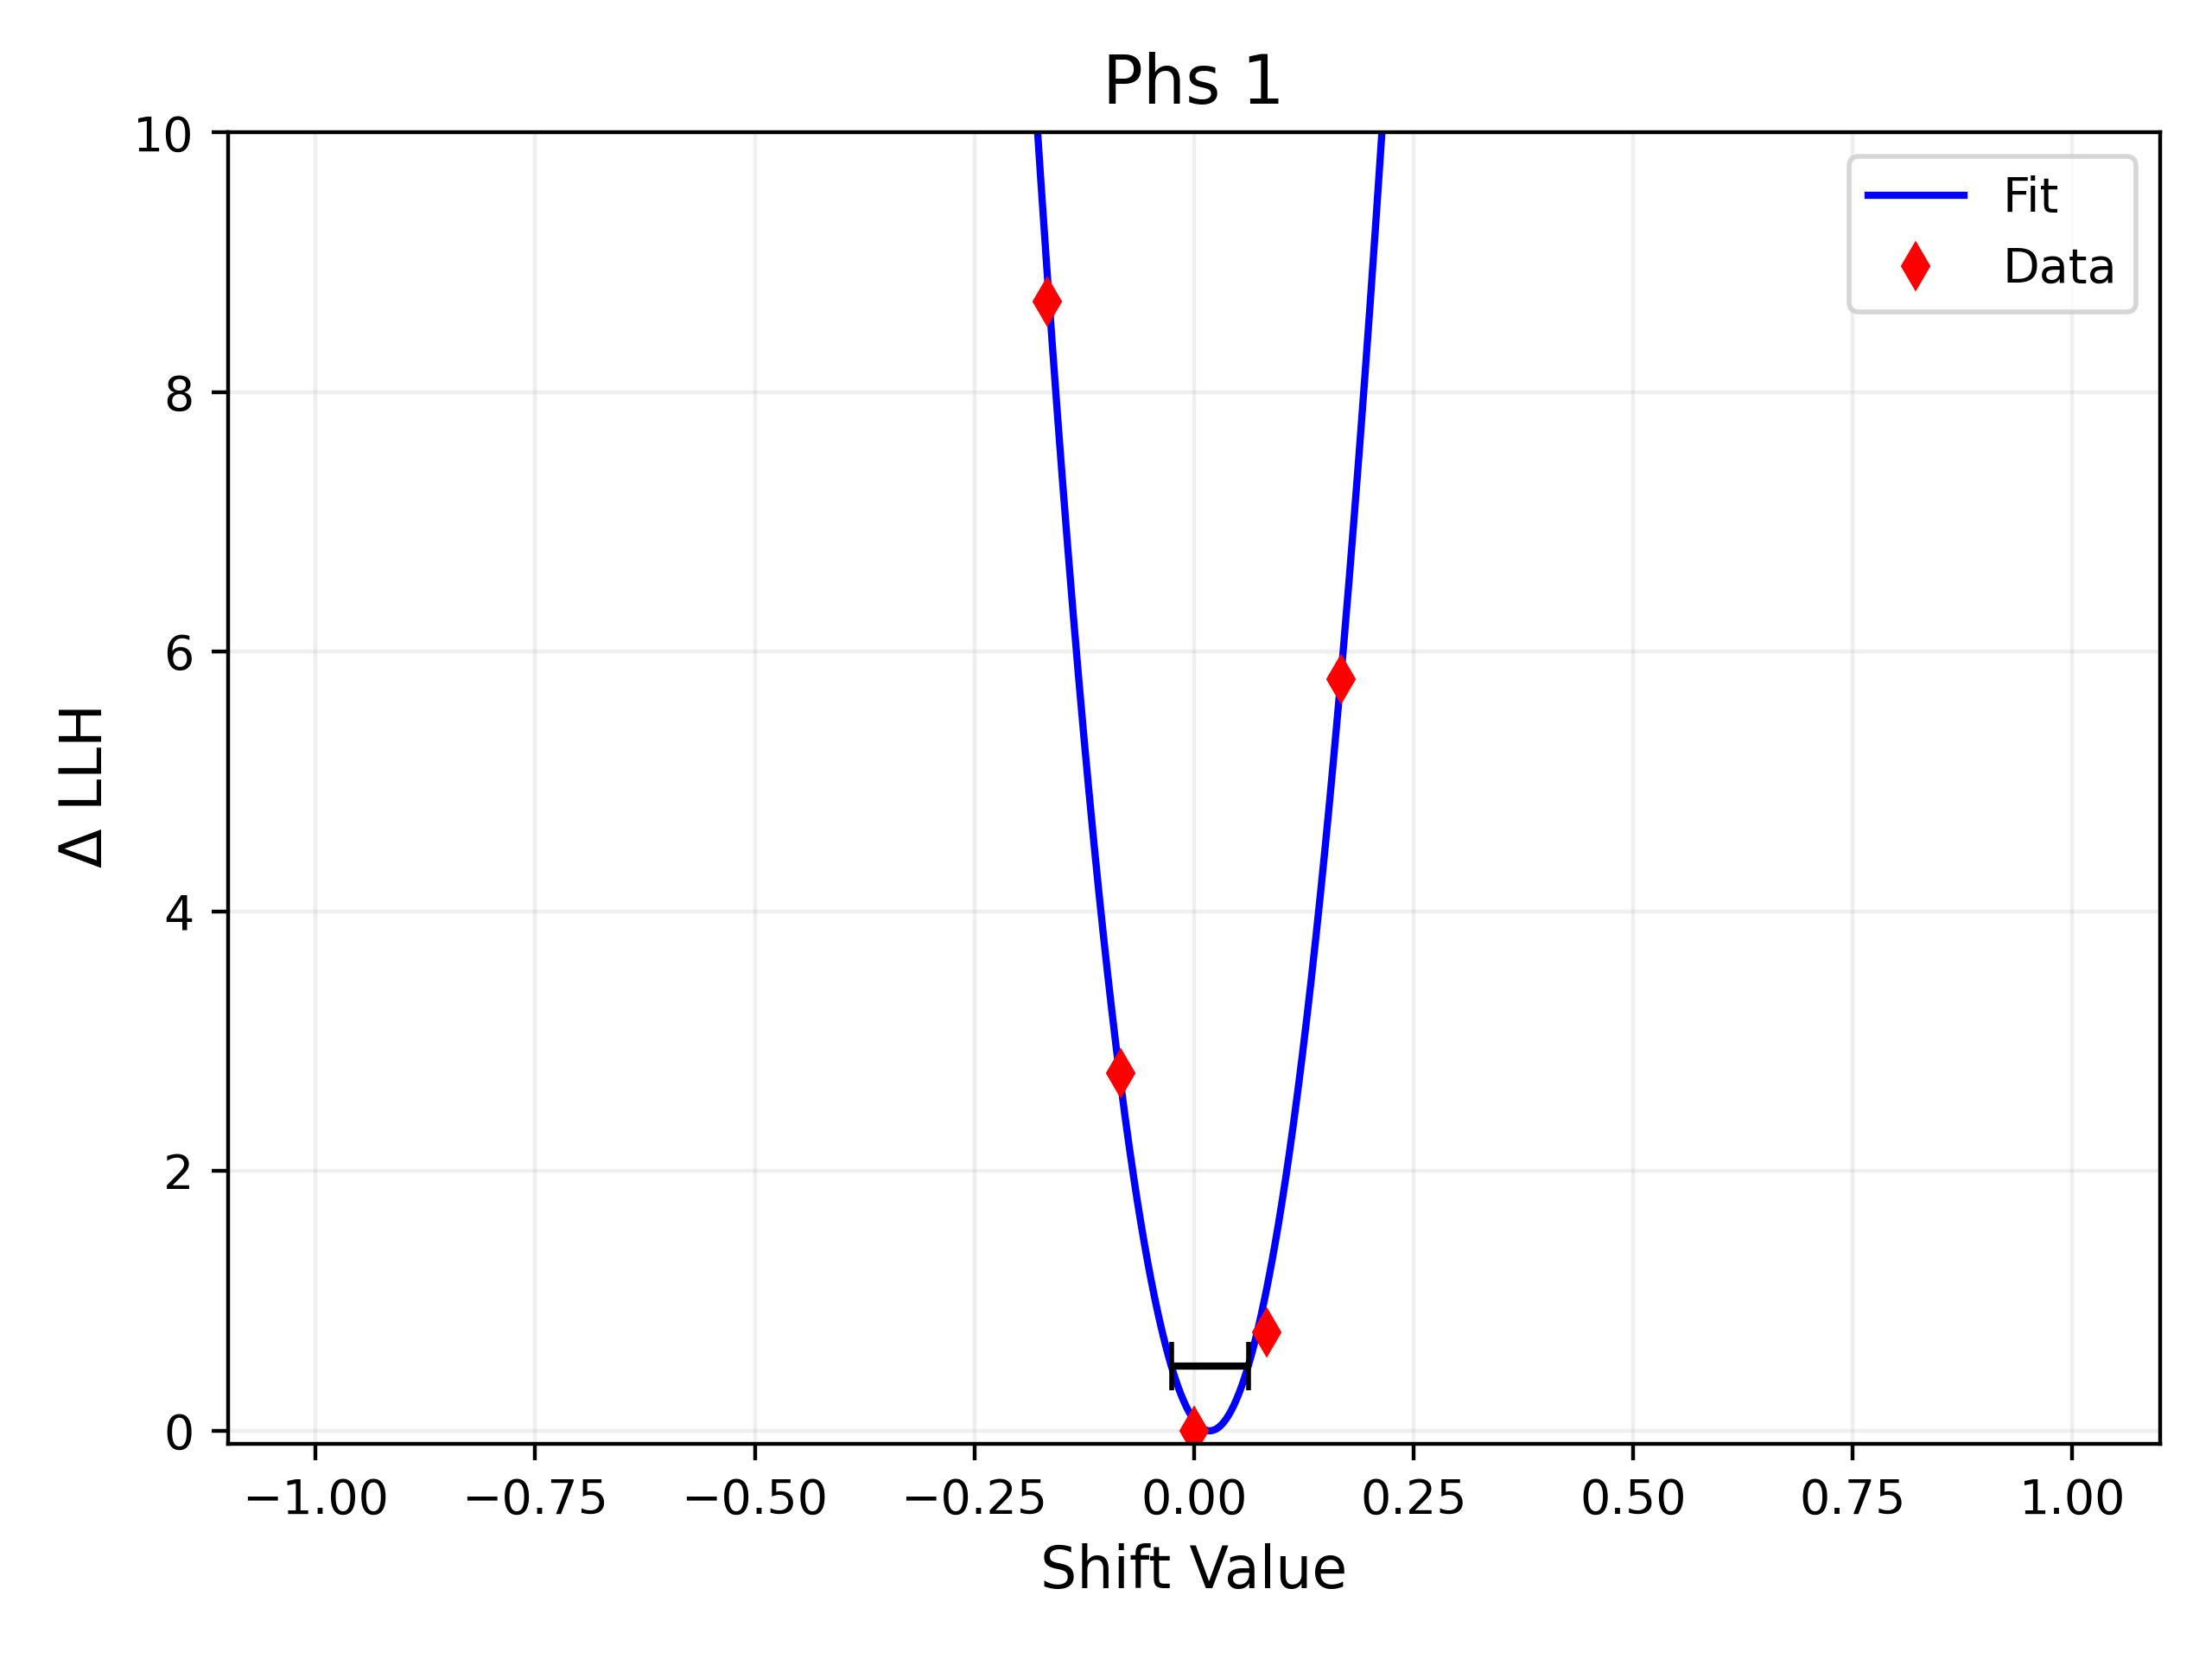
\includegraphics[width=0.3\linewidth]{figures/ice_fits/Phs_1_llhfunc.png}\\
    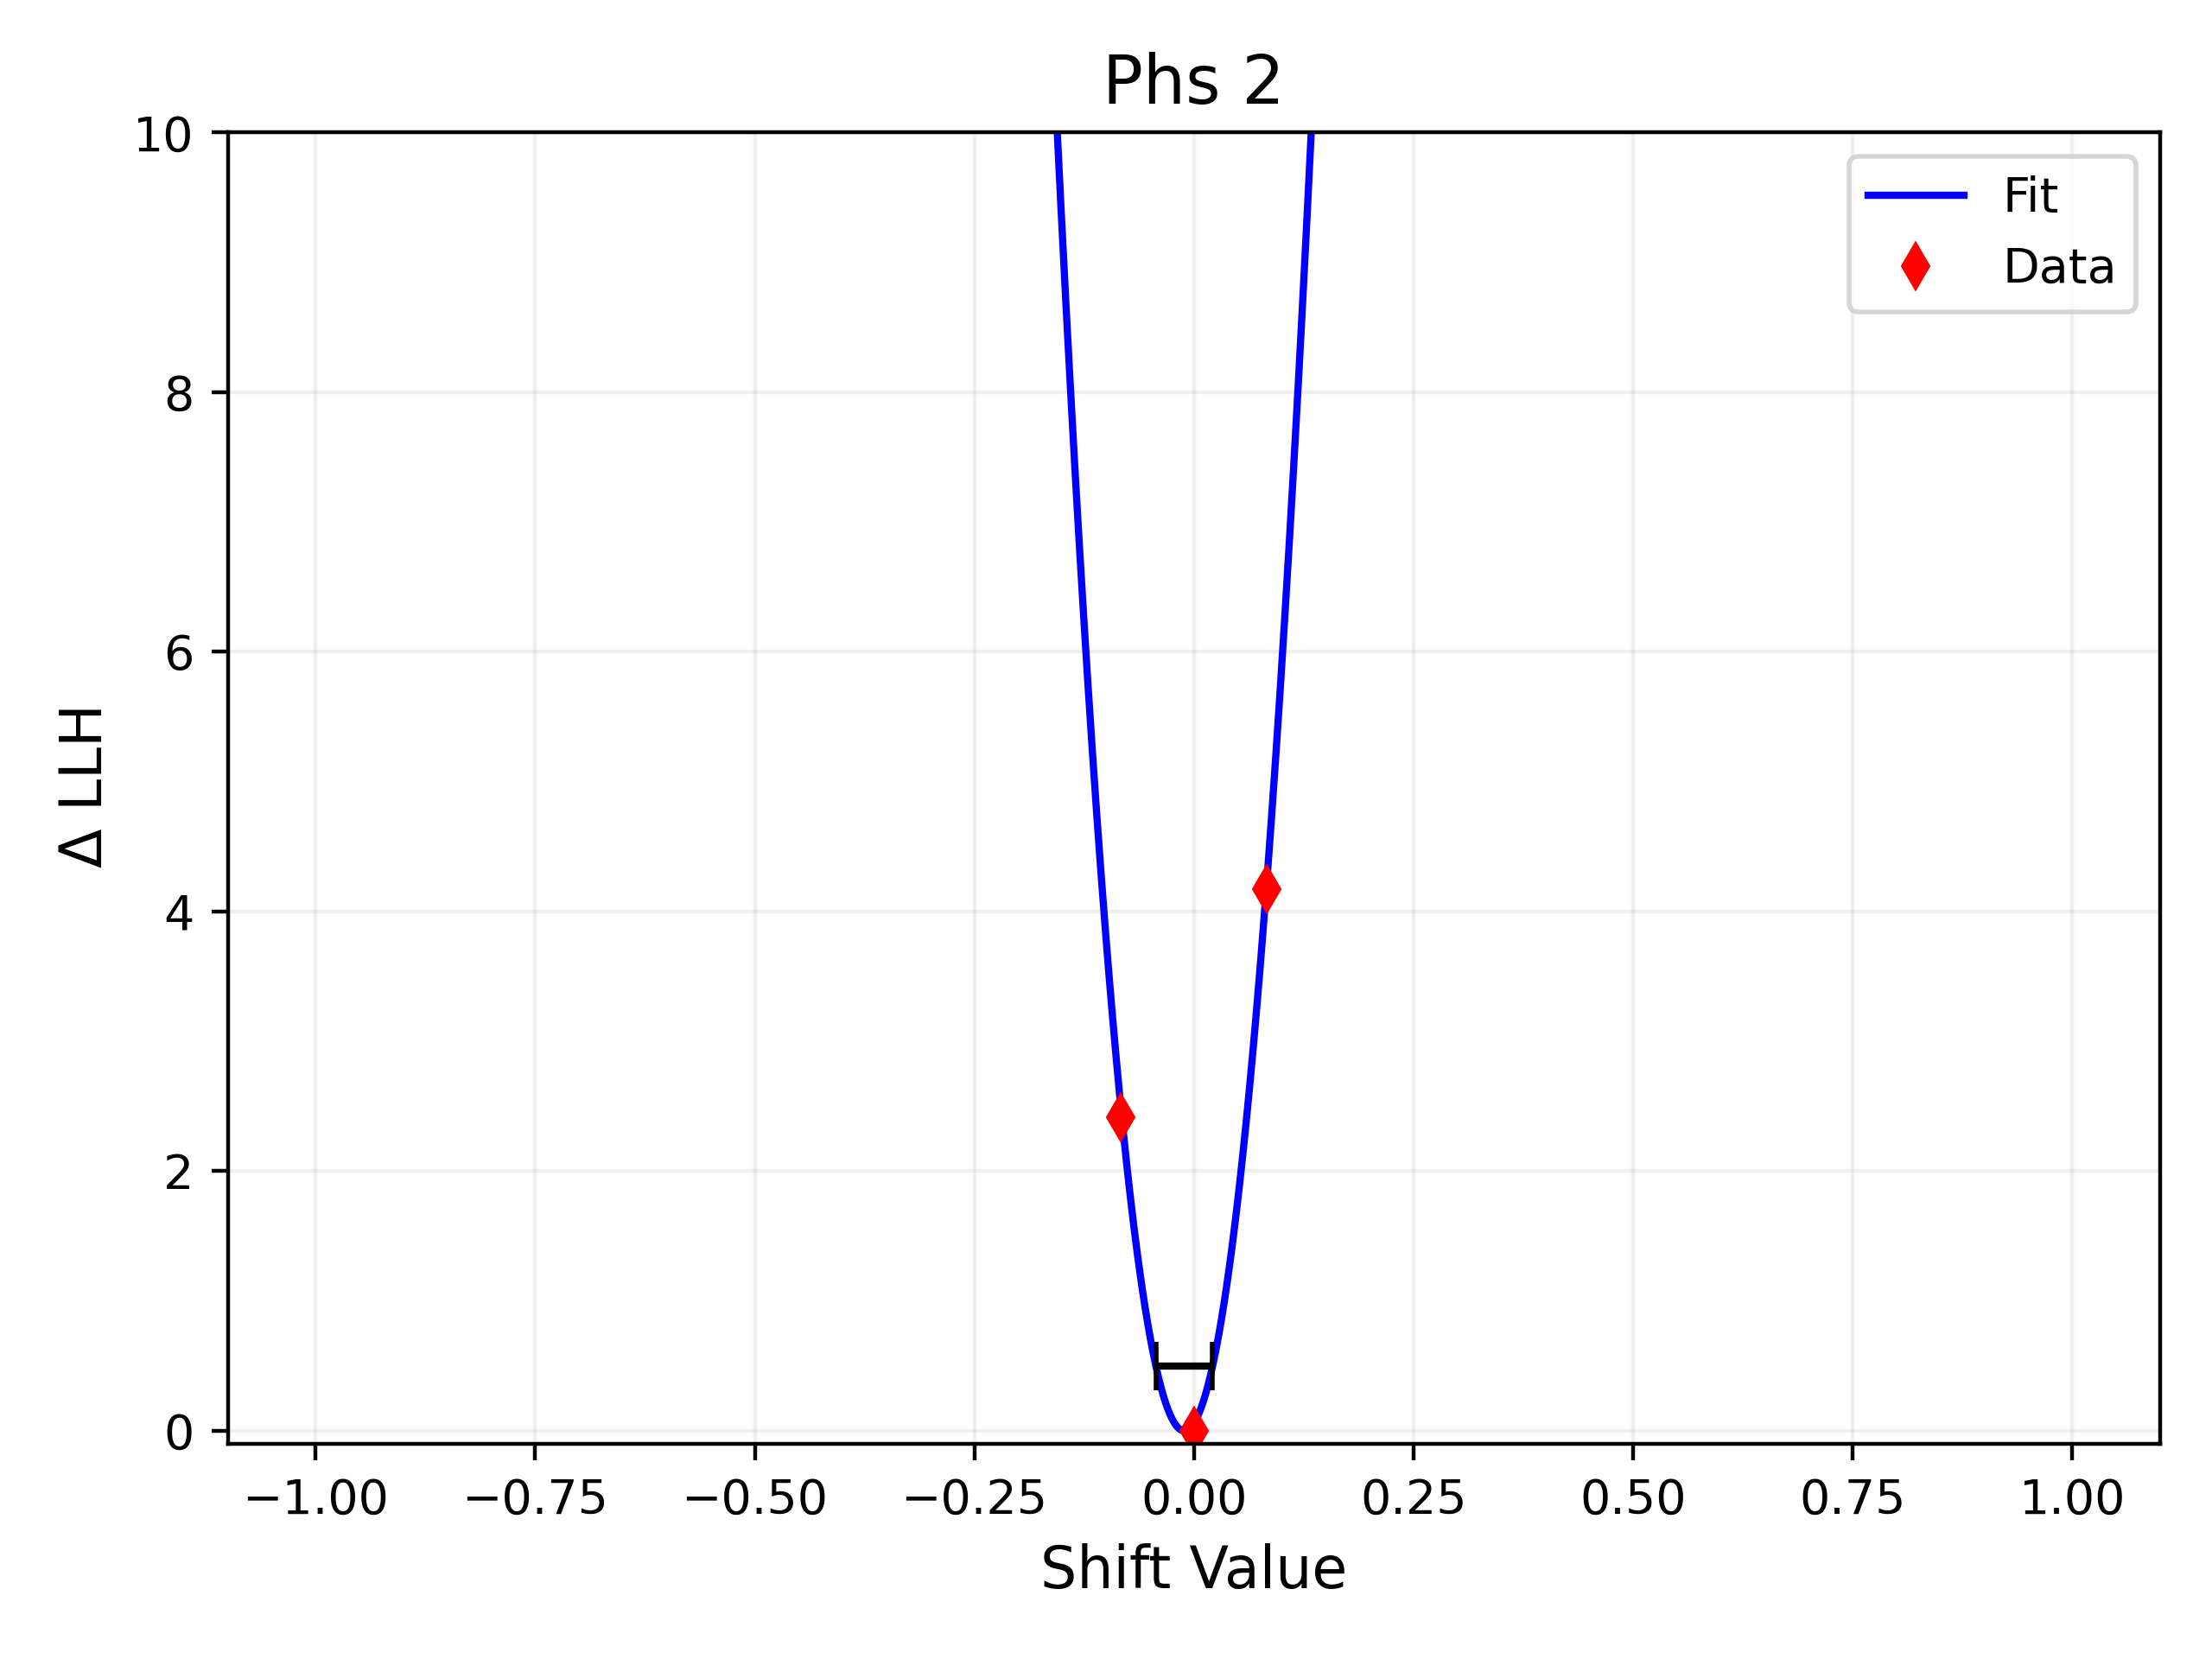
\includegraphics[width=0.3\linewidth]{figures/ice_fits/Phs_2_llhfunc.png}%
    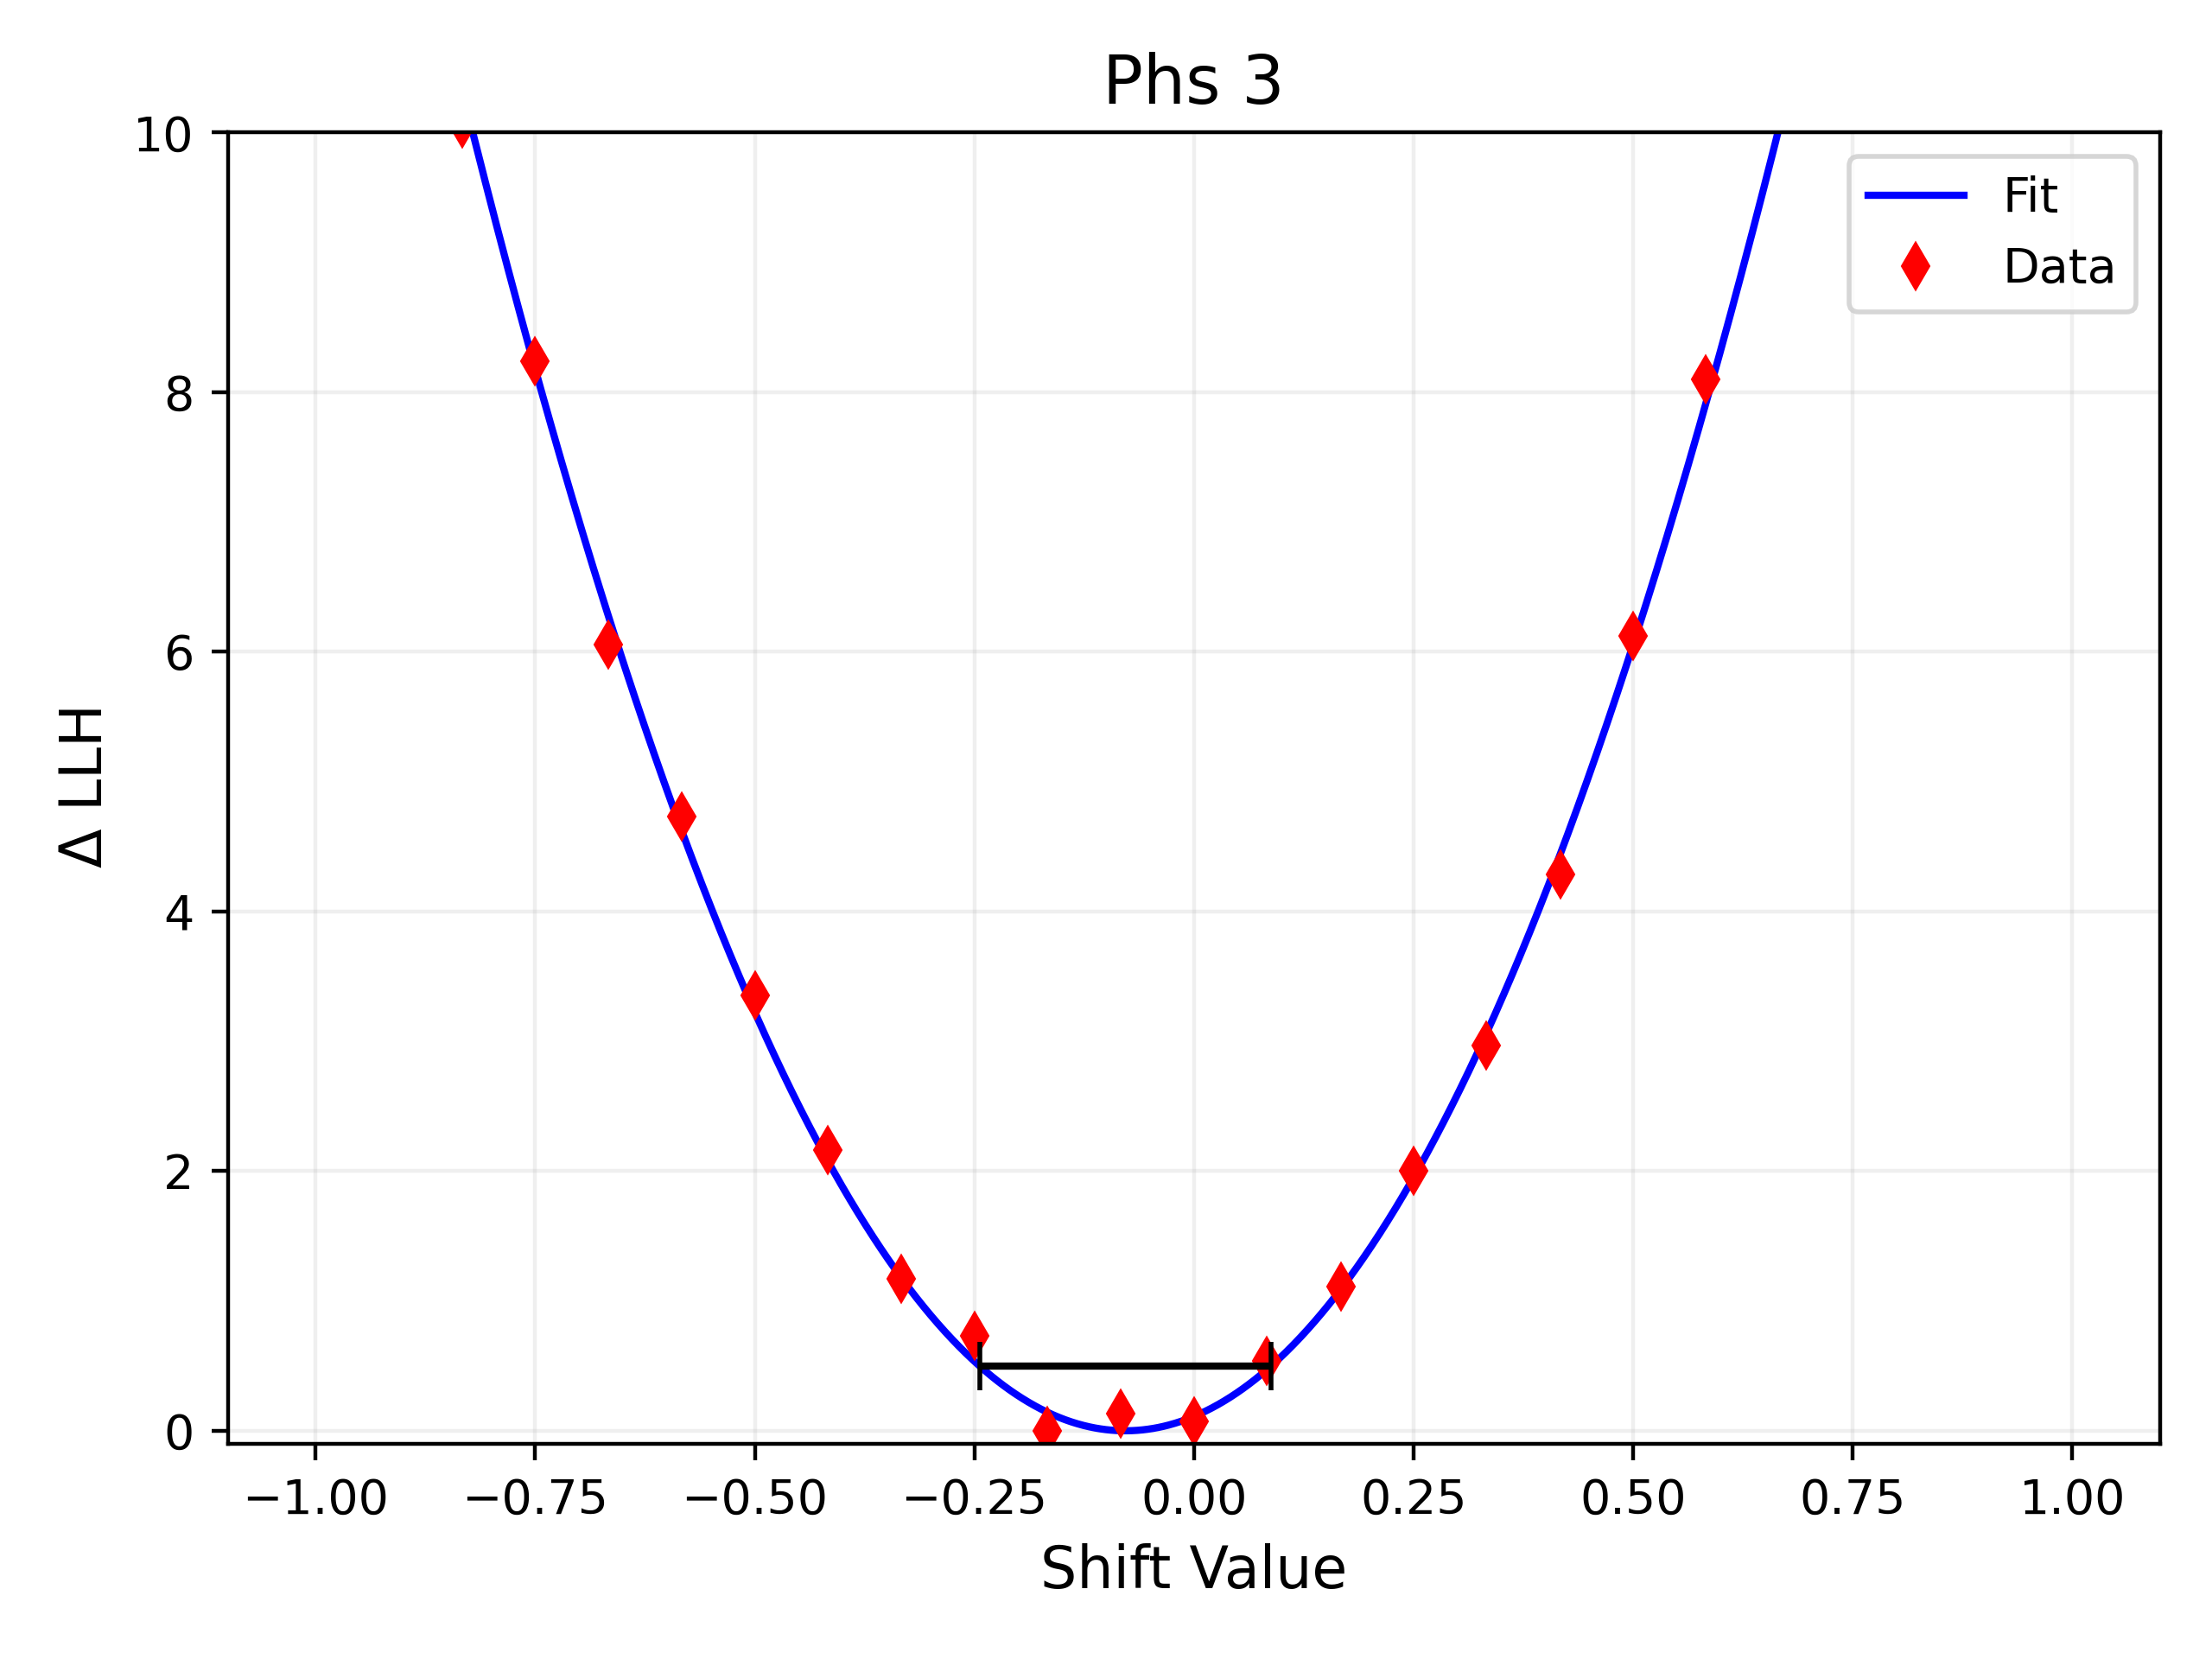
\includegraphics[width=0.3\linewidth]{figures/ice_fits/Phs_3_llhfunc.png}%
    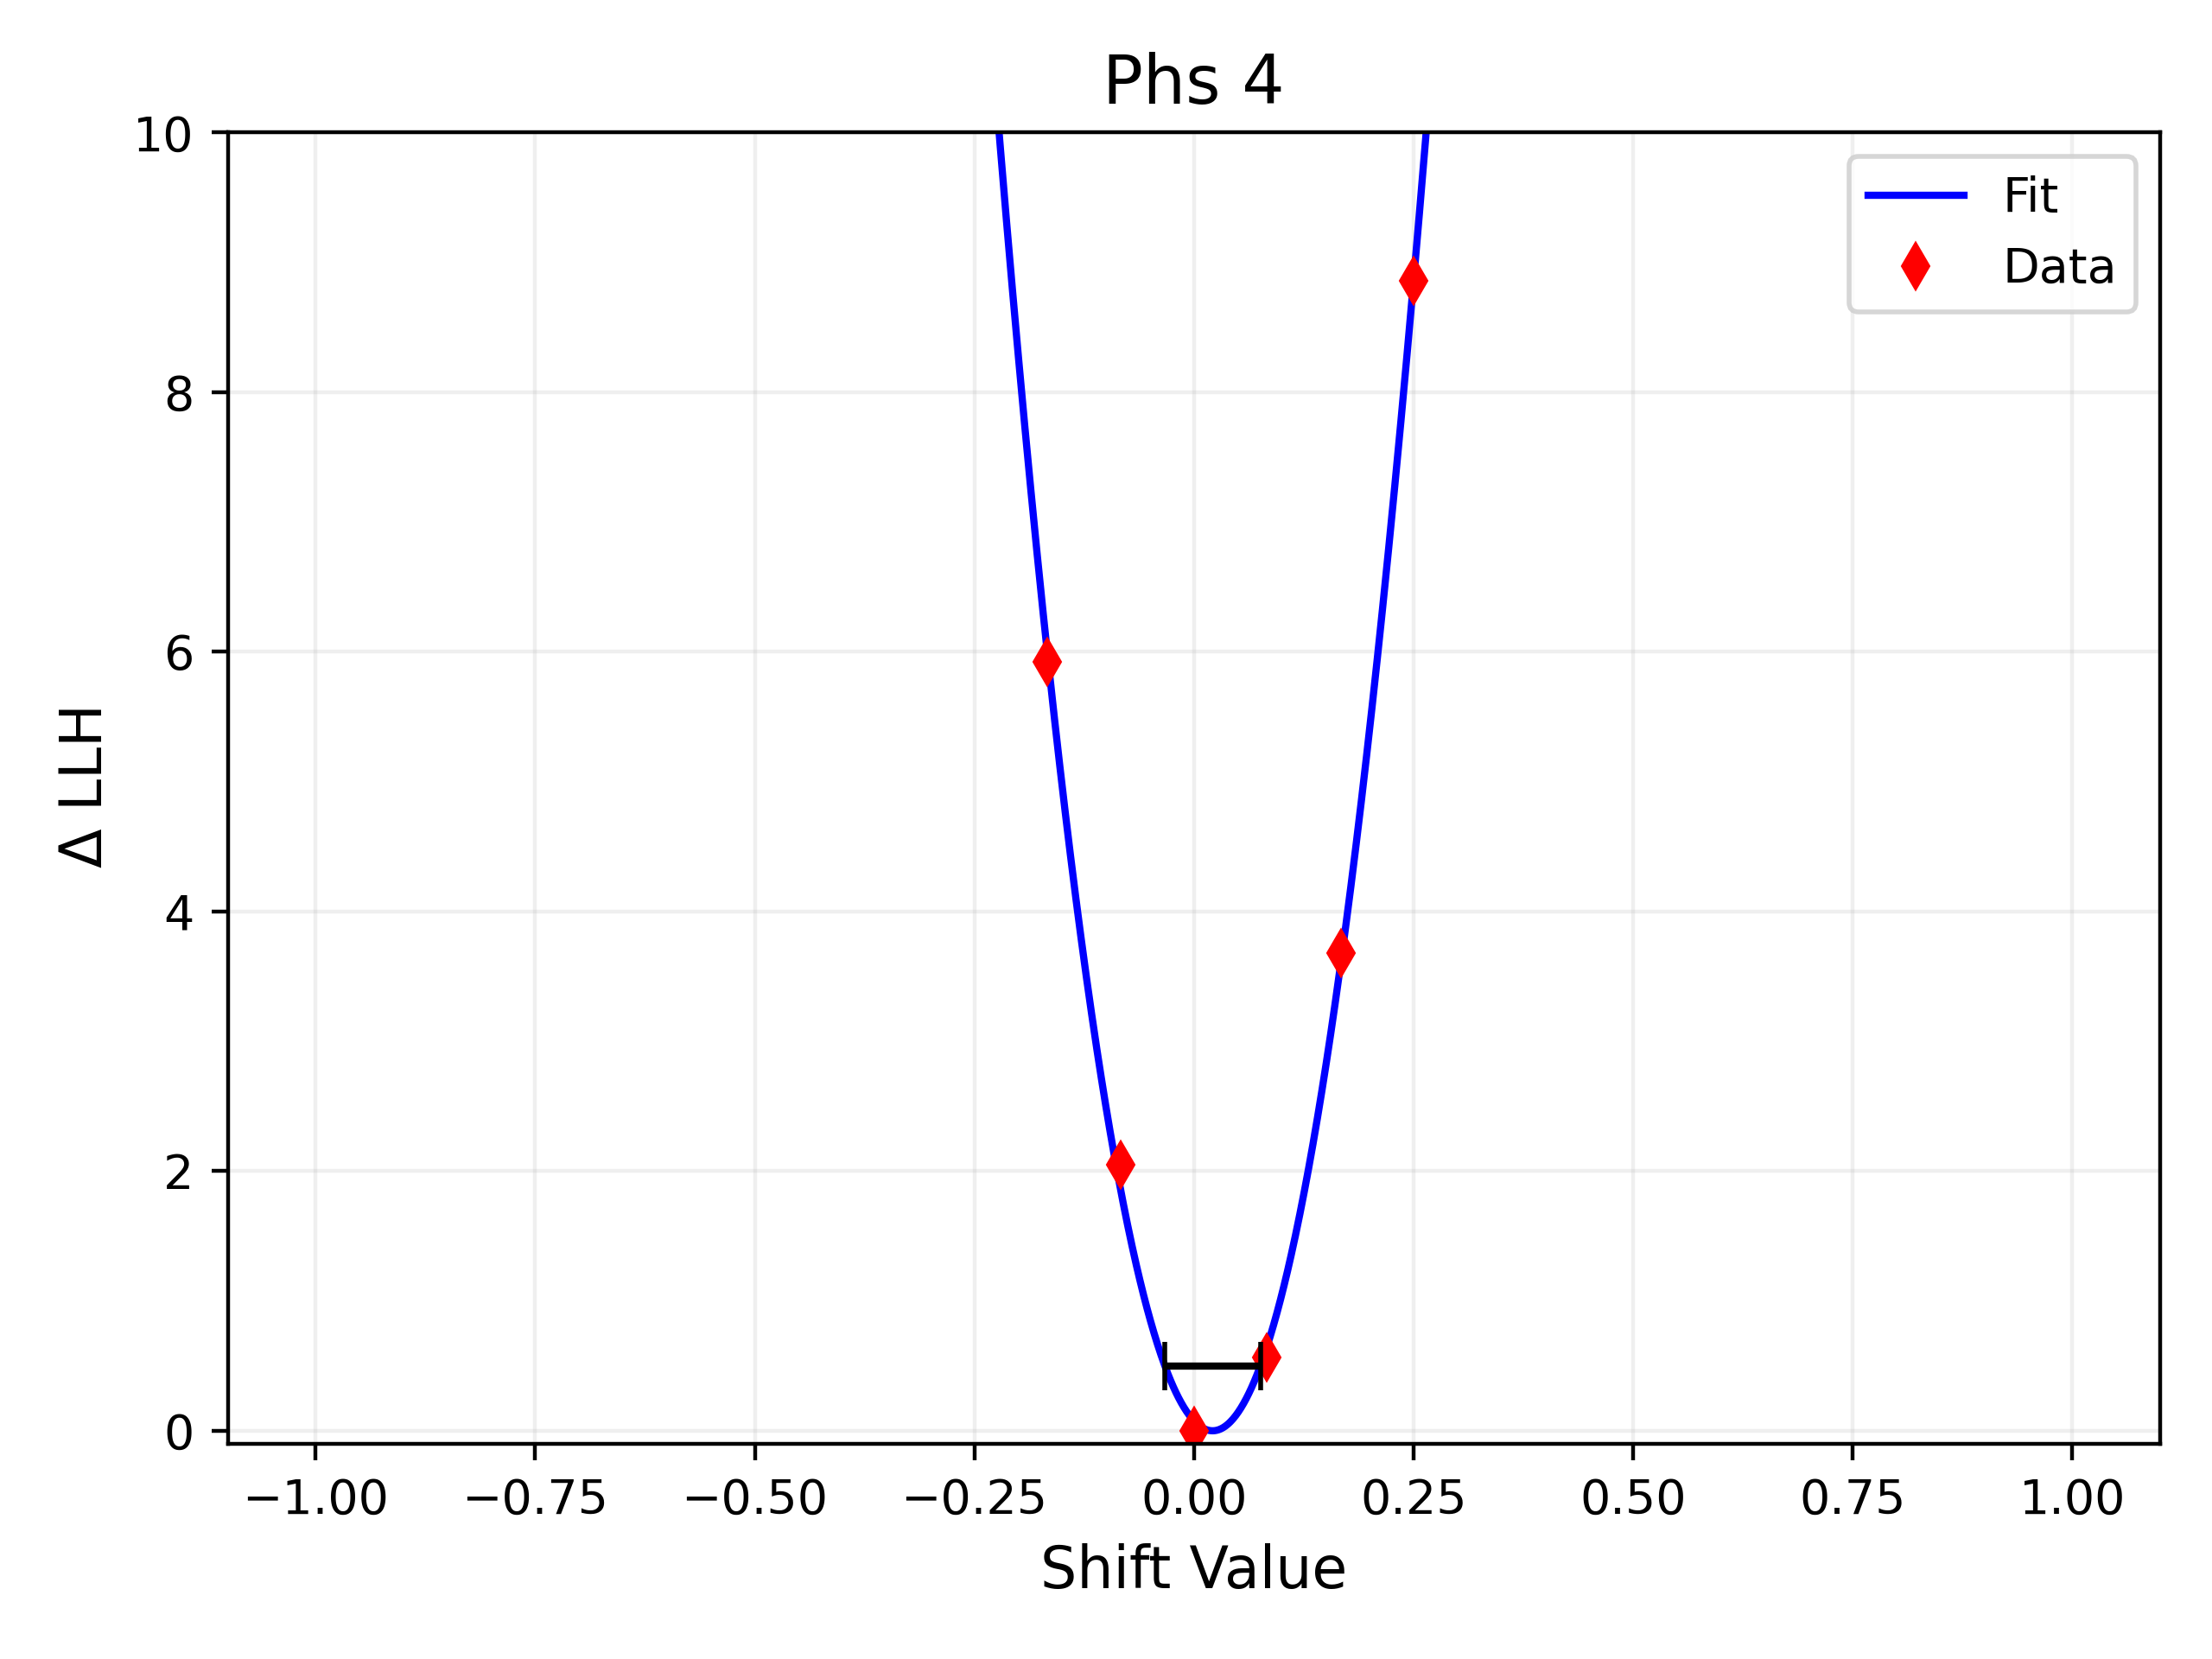
\includegraphics[width=0.3\linewidth]{figures/ice_fits/Phs_4_llhfunc.png}
    \caption{The first five amplitude fits and the first four phase fits for the plus-mode Fourier series decomposition. `Shift Value' corresponds to the difference of the best fit value from the PPC simulations to the previous best-fit value for the parameter. The black line at 0.5 $\Delta LLH$ represents the $1\sigma$ uncertainty band.}\label{fig:linearfit}
\end{figure}

For a normally-distributed, correlated, set of nuisance parameters $\vec{\eta}$, the prior penalty of the likelihood function is equal to 
\begin{equation}
    \mathcal{L} = \vec{\eta}^{T} \Sigma^{-1} \vec{\eta} + C
\end{equation} 
where $C$ is a constant prefactor to normalize the distribution and $\Sigma$ is the covariance matrix.
The inverse of the covariance matrix, $\Sigma^{-1}$ is also known as the Hessian matrix; in determining the covariance it is easiest to first directly fit to the Hessian, and then to invert the Hessian to get the covariance matrix.
In order for the prior penalty function to normalizable, both the covariance matrix and the hessian must be real-valued and positive semi-definite: all eigenvalues and its determinant must be greater than or equal to zero. 
A consequence of this, and the use of a Cholesky decomposition, is that the Hessian can be written as the matrix product of a lower-diagonal matrix and its transpose:
\begin{equation}
    \Sigma^{-1} = H = LL^{T},
\end{equation} 
where $L$ is some lower-diagonal matrix. 
We can therefore parametrize any Hessian matrix $H$ using values occupying the lower-diagonal of such a matrix $L$. This takes $n(n-1)/2$ values, where $n$ is the rank of the covariance. 

We use the Cauchy robust loss function as a metric for the fits, in which we minimize the lower-diagonal matrix $\bvec{L}$,
\begin{equation}
    M(\bvec{L}) = \sum_{i}^{m}\log\left[ 1 +  \left(\mathcal{L}_{i} - \tfrac{1}{2}(\vec{\eta}_{i})^{T} \bvec{L}\bvec{L}^{T} \vec{\eta}_ {i} \right)^{2}\right]
\end{equation}
for the $m$ sampled ice models where $\vec{\eta}_{i}$ is the $i$'th sampled set of nuisance parameters at which a log likelihood of $\mathcal{L}_{i}$ was recovered through PPC simulation. 
This likelihood function, which has been used in previous IceCube analyses~\cite{icecube_lowe}, was chosen such that bad fits far off the true likelihood contours do not negatively affect the fit.  
The fit, despite running over forty-five parameters, was found to be extremely stable and fast. The fit Hessian $H=\bvec{L}\bvec{L}^{T}$ is show in Figure~\ref{fig:hessian} (left) and the correlation matrix (right).
\begin{figure}
    \centering
    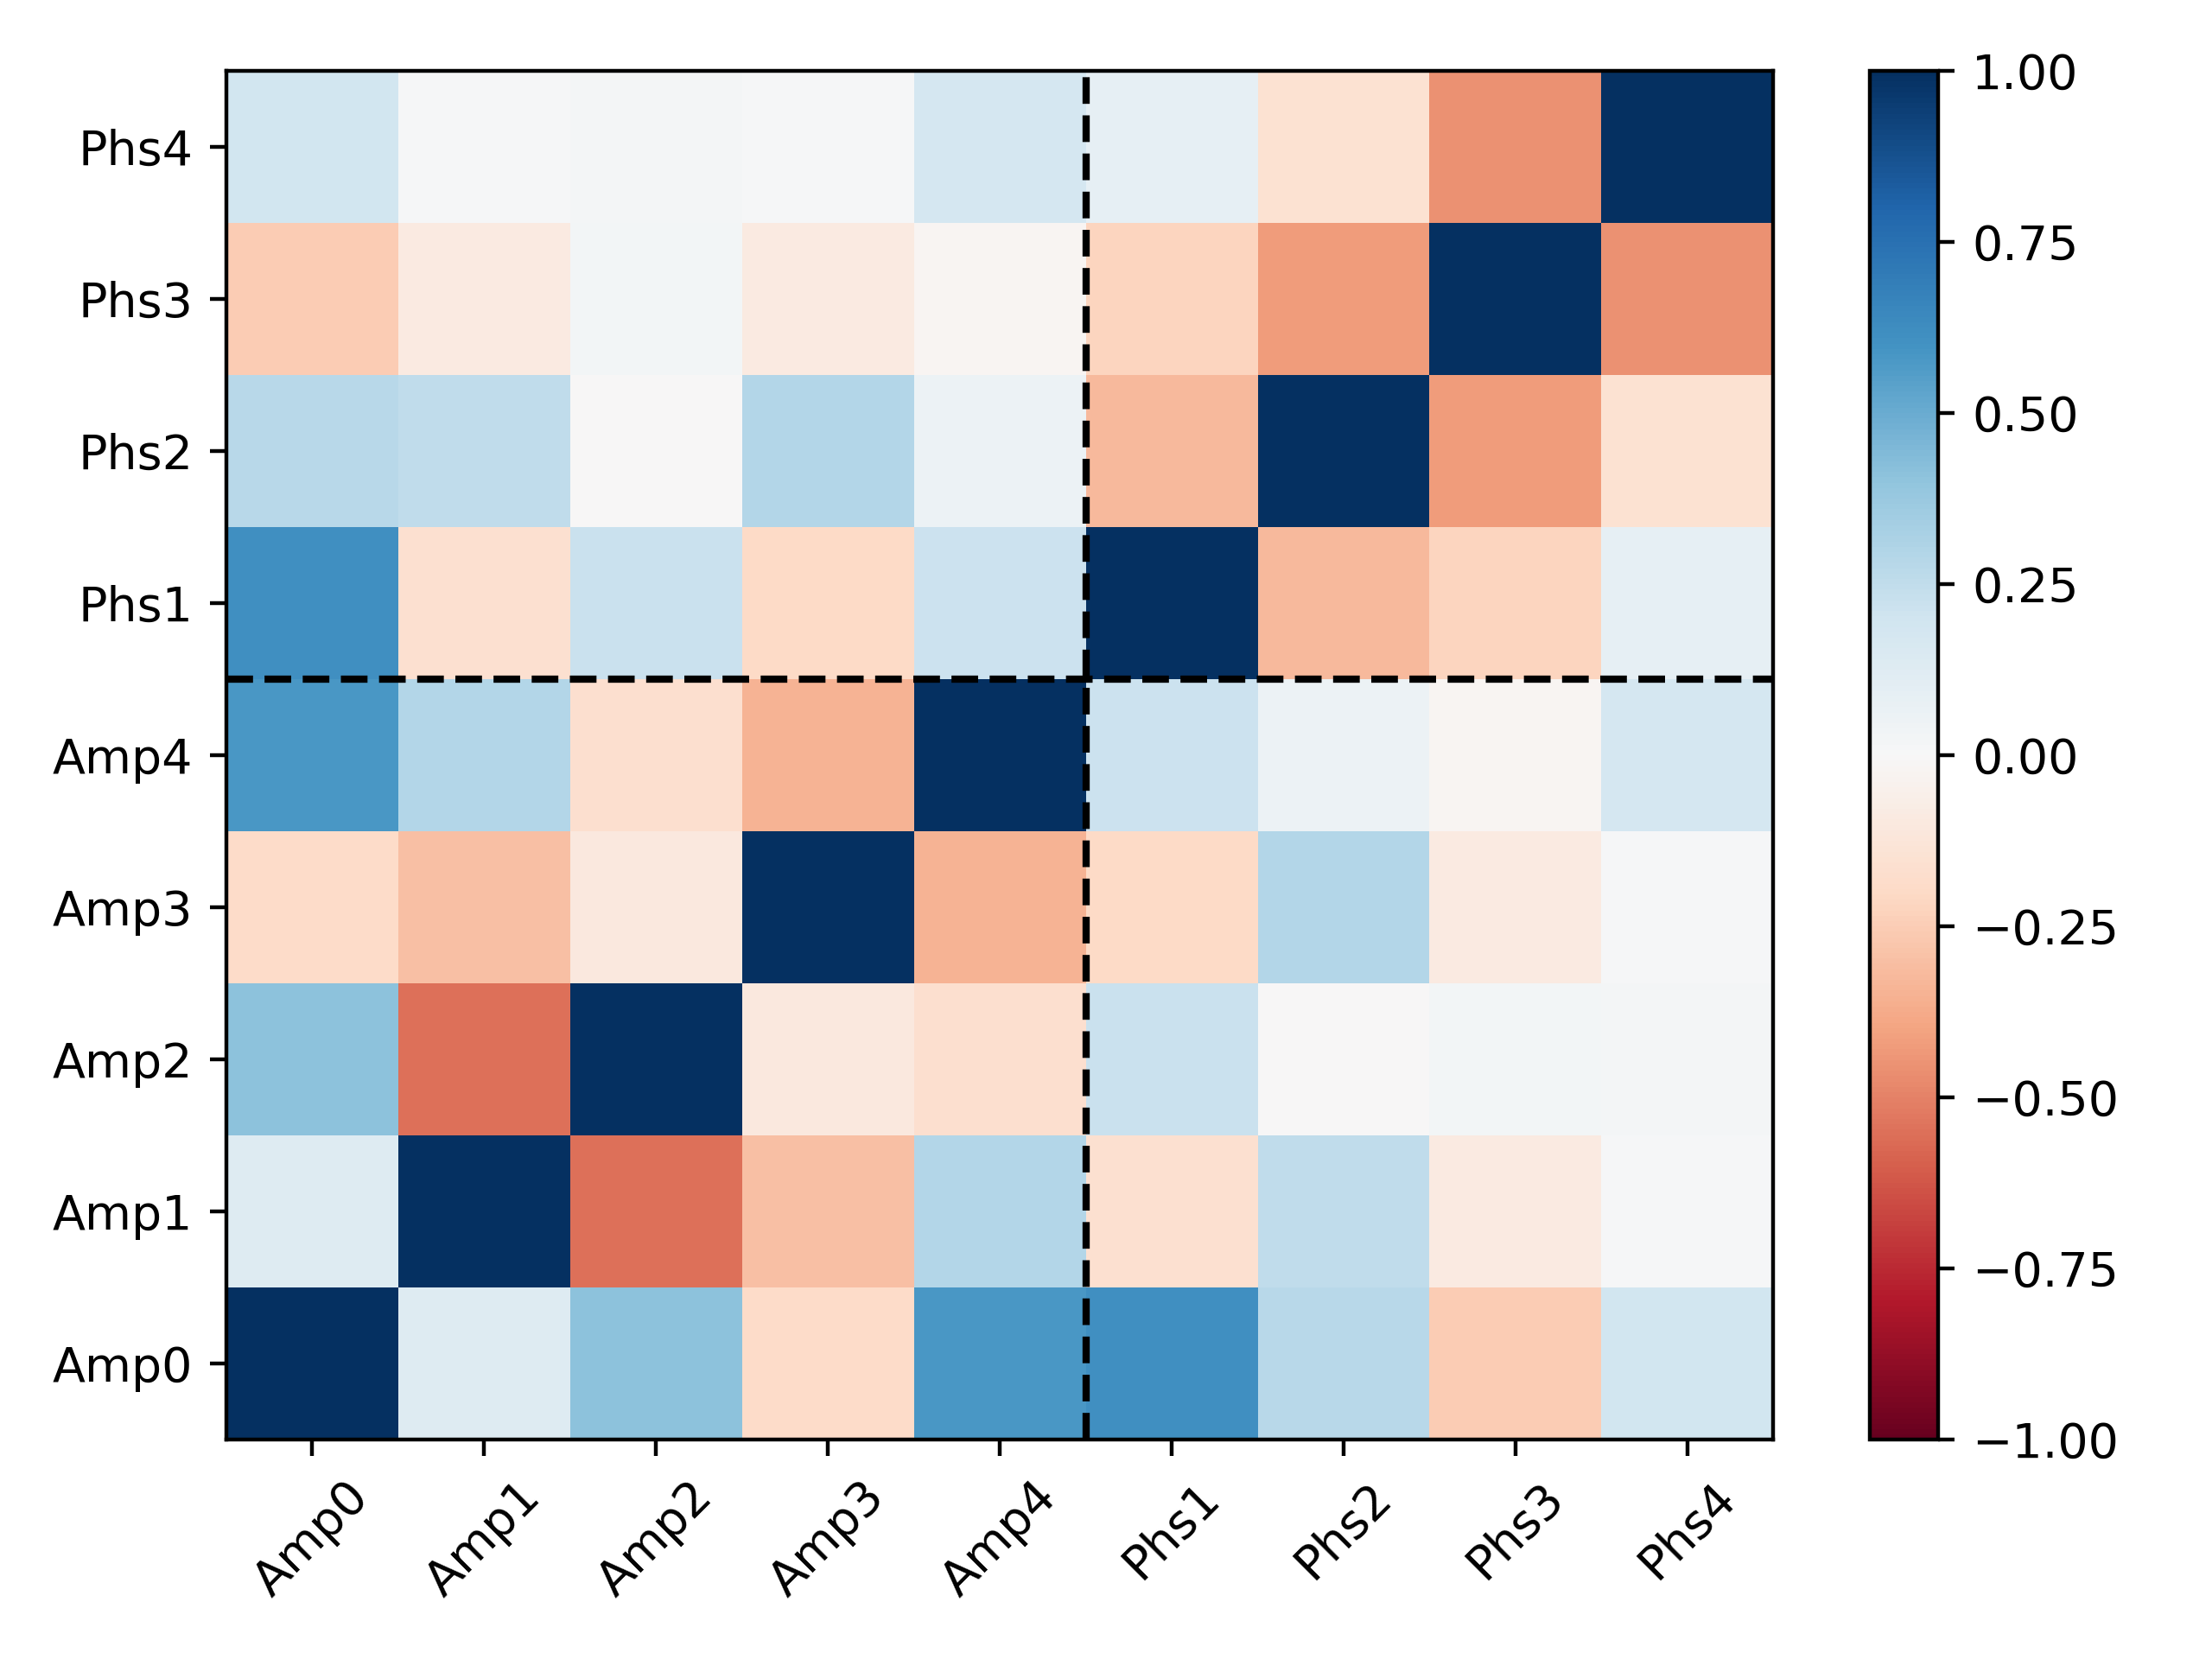
\includegraphics[width=0.45\linewidth]{figures/hessian.png}%
    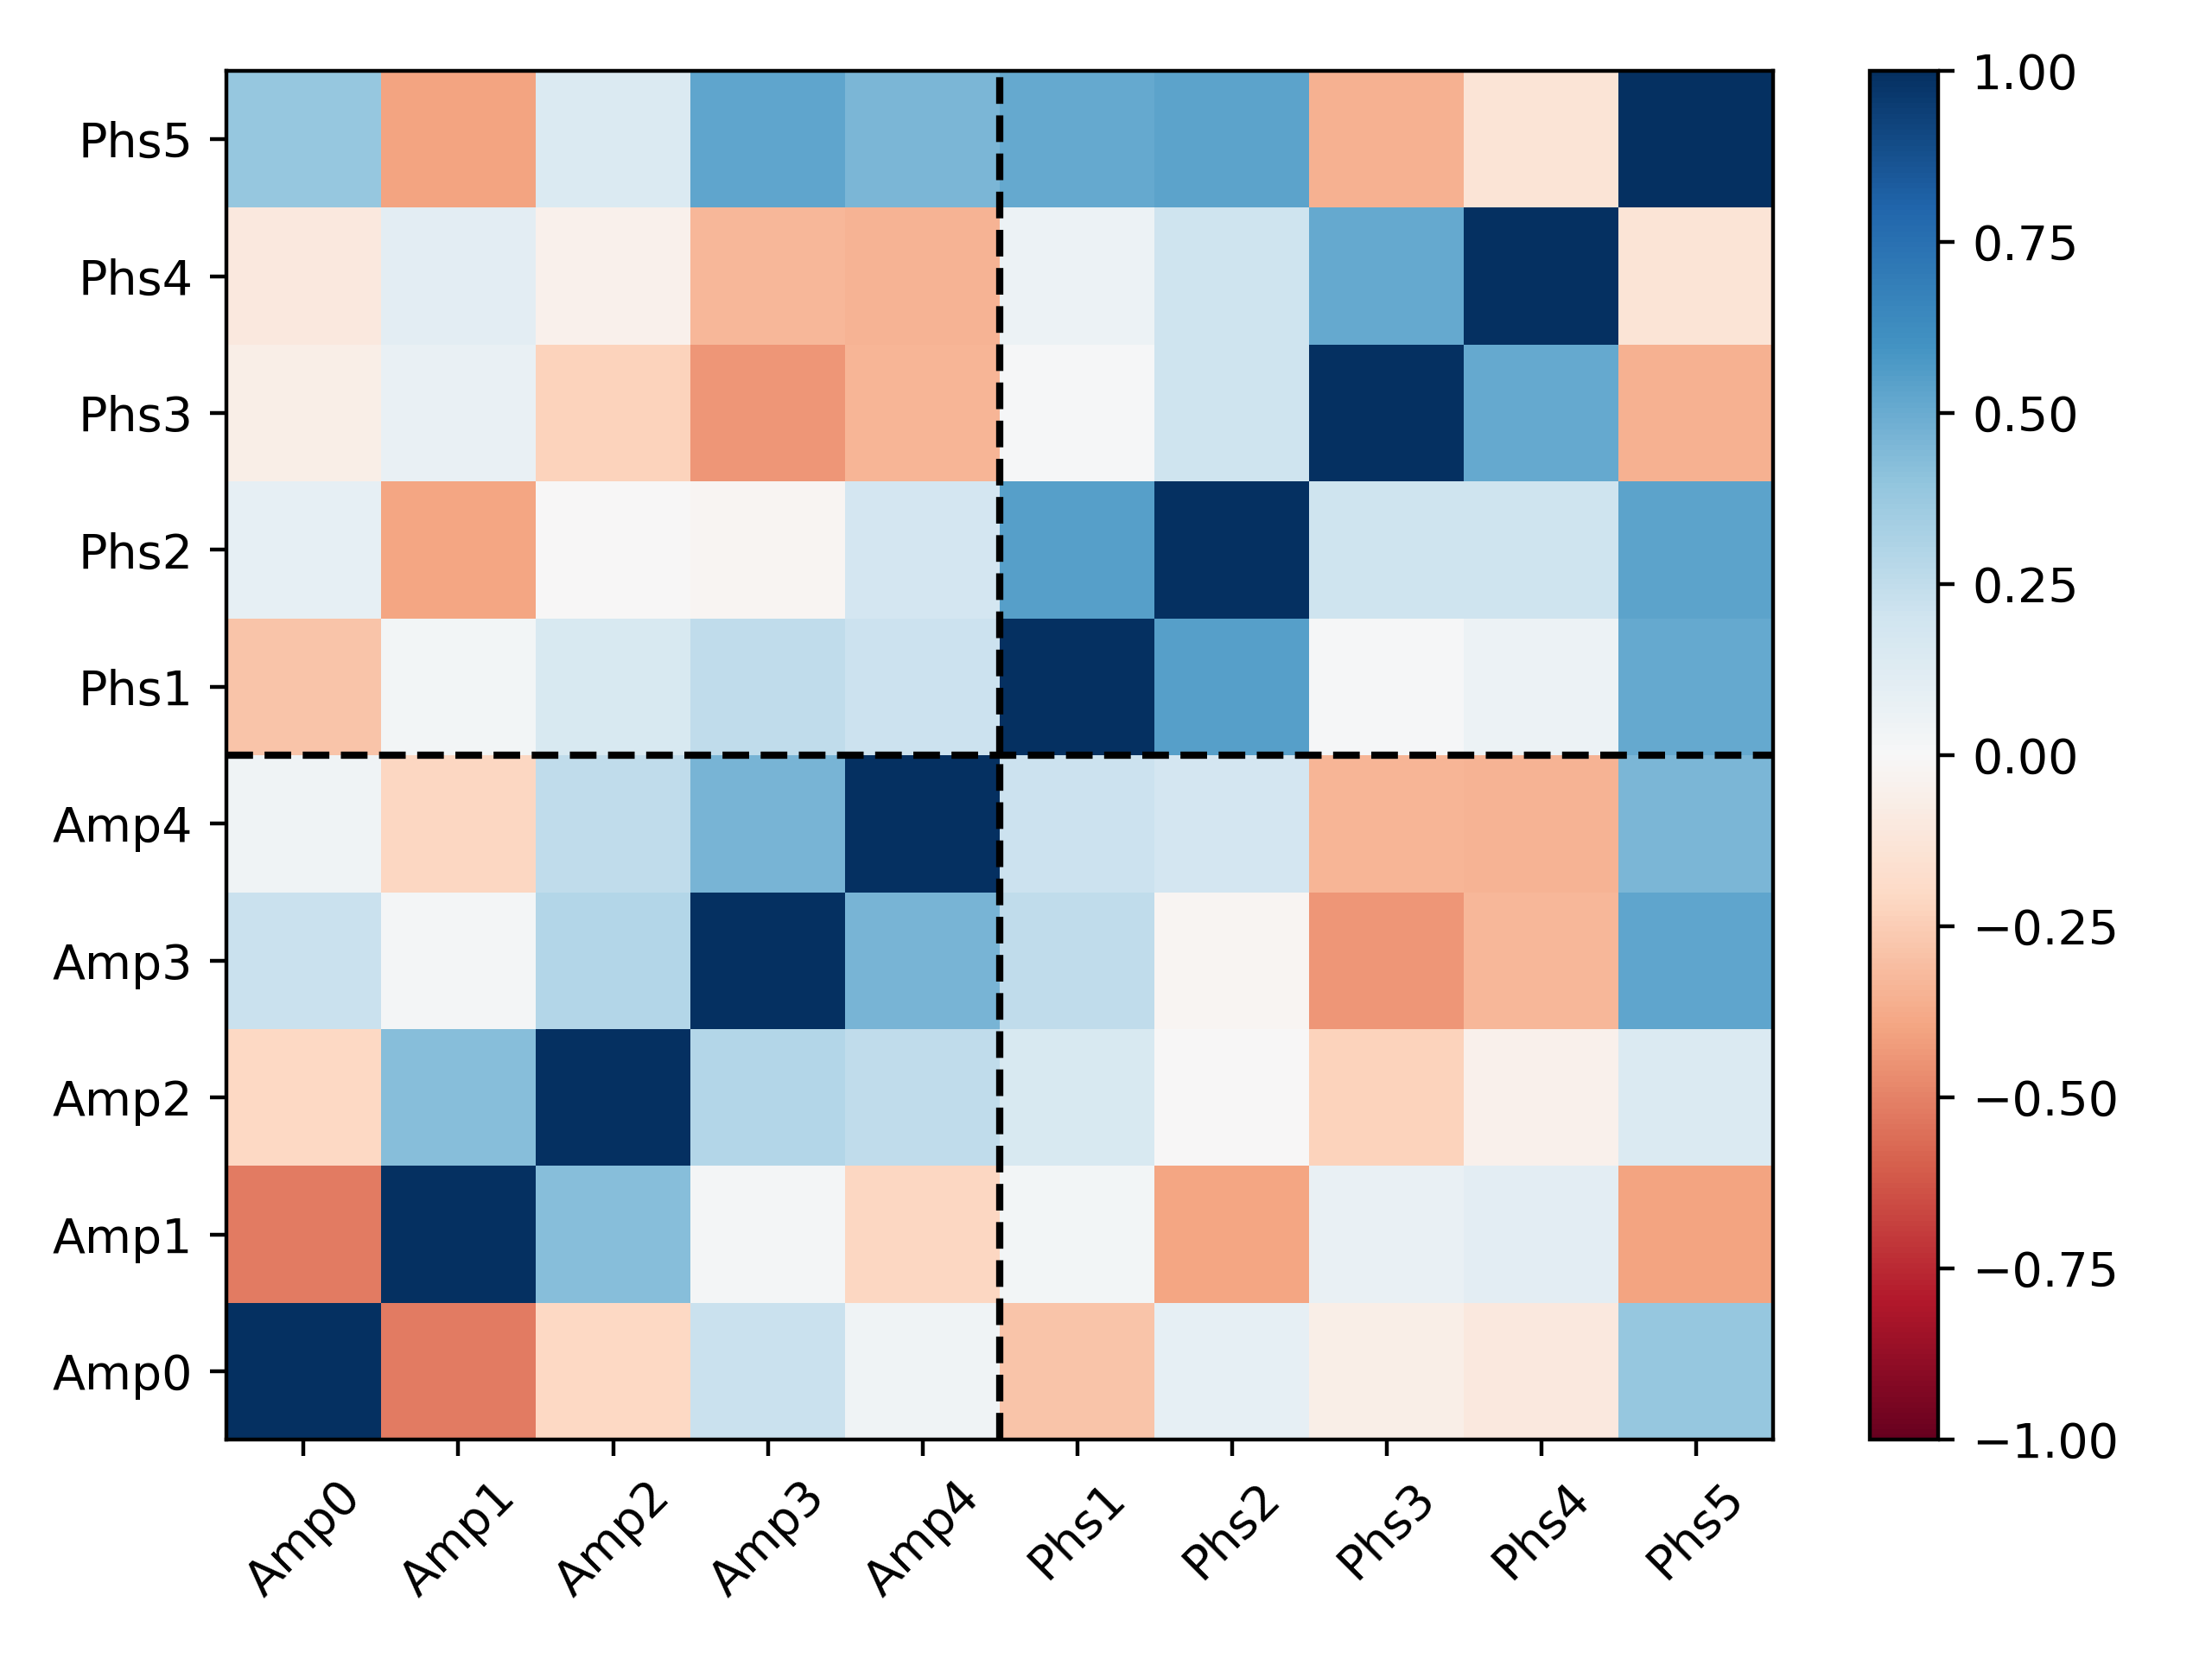
\includegraphics[width=0.45\linewidth]{figures/covariance.png}
    \caption{The fit hessian matrix (left) in nuisance parameter space for the first five amplitudes and first four phases, and the correlation matrix (right) determined by inverting the hessian.}\label{fig:hessian}
\end{figure}

Using these the expected variation of ice models can be calculated. 
Five thousand random ice models were drawn, using the correlation matrix and the fit widths of the amplitudes and phases, and are shown in Figure~\ref{fig:envelope}.

\begin{figure}
    \centering
    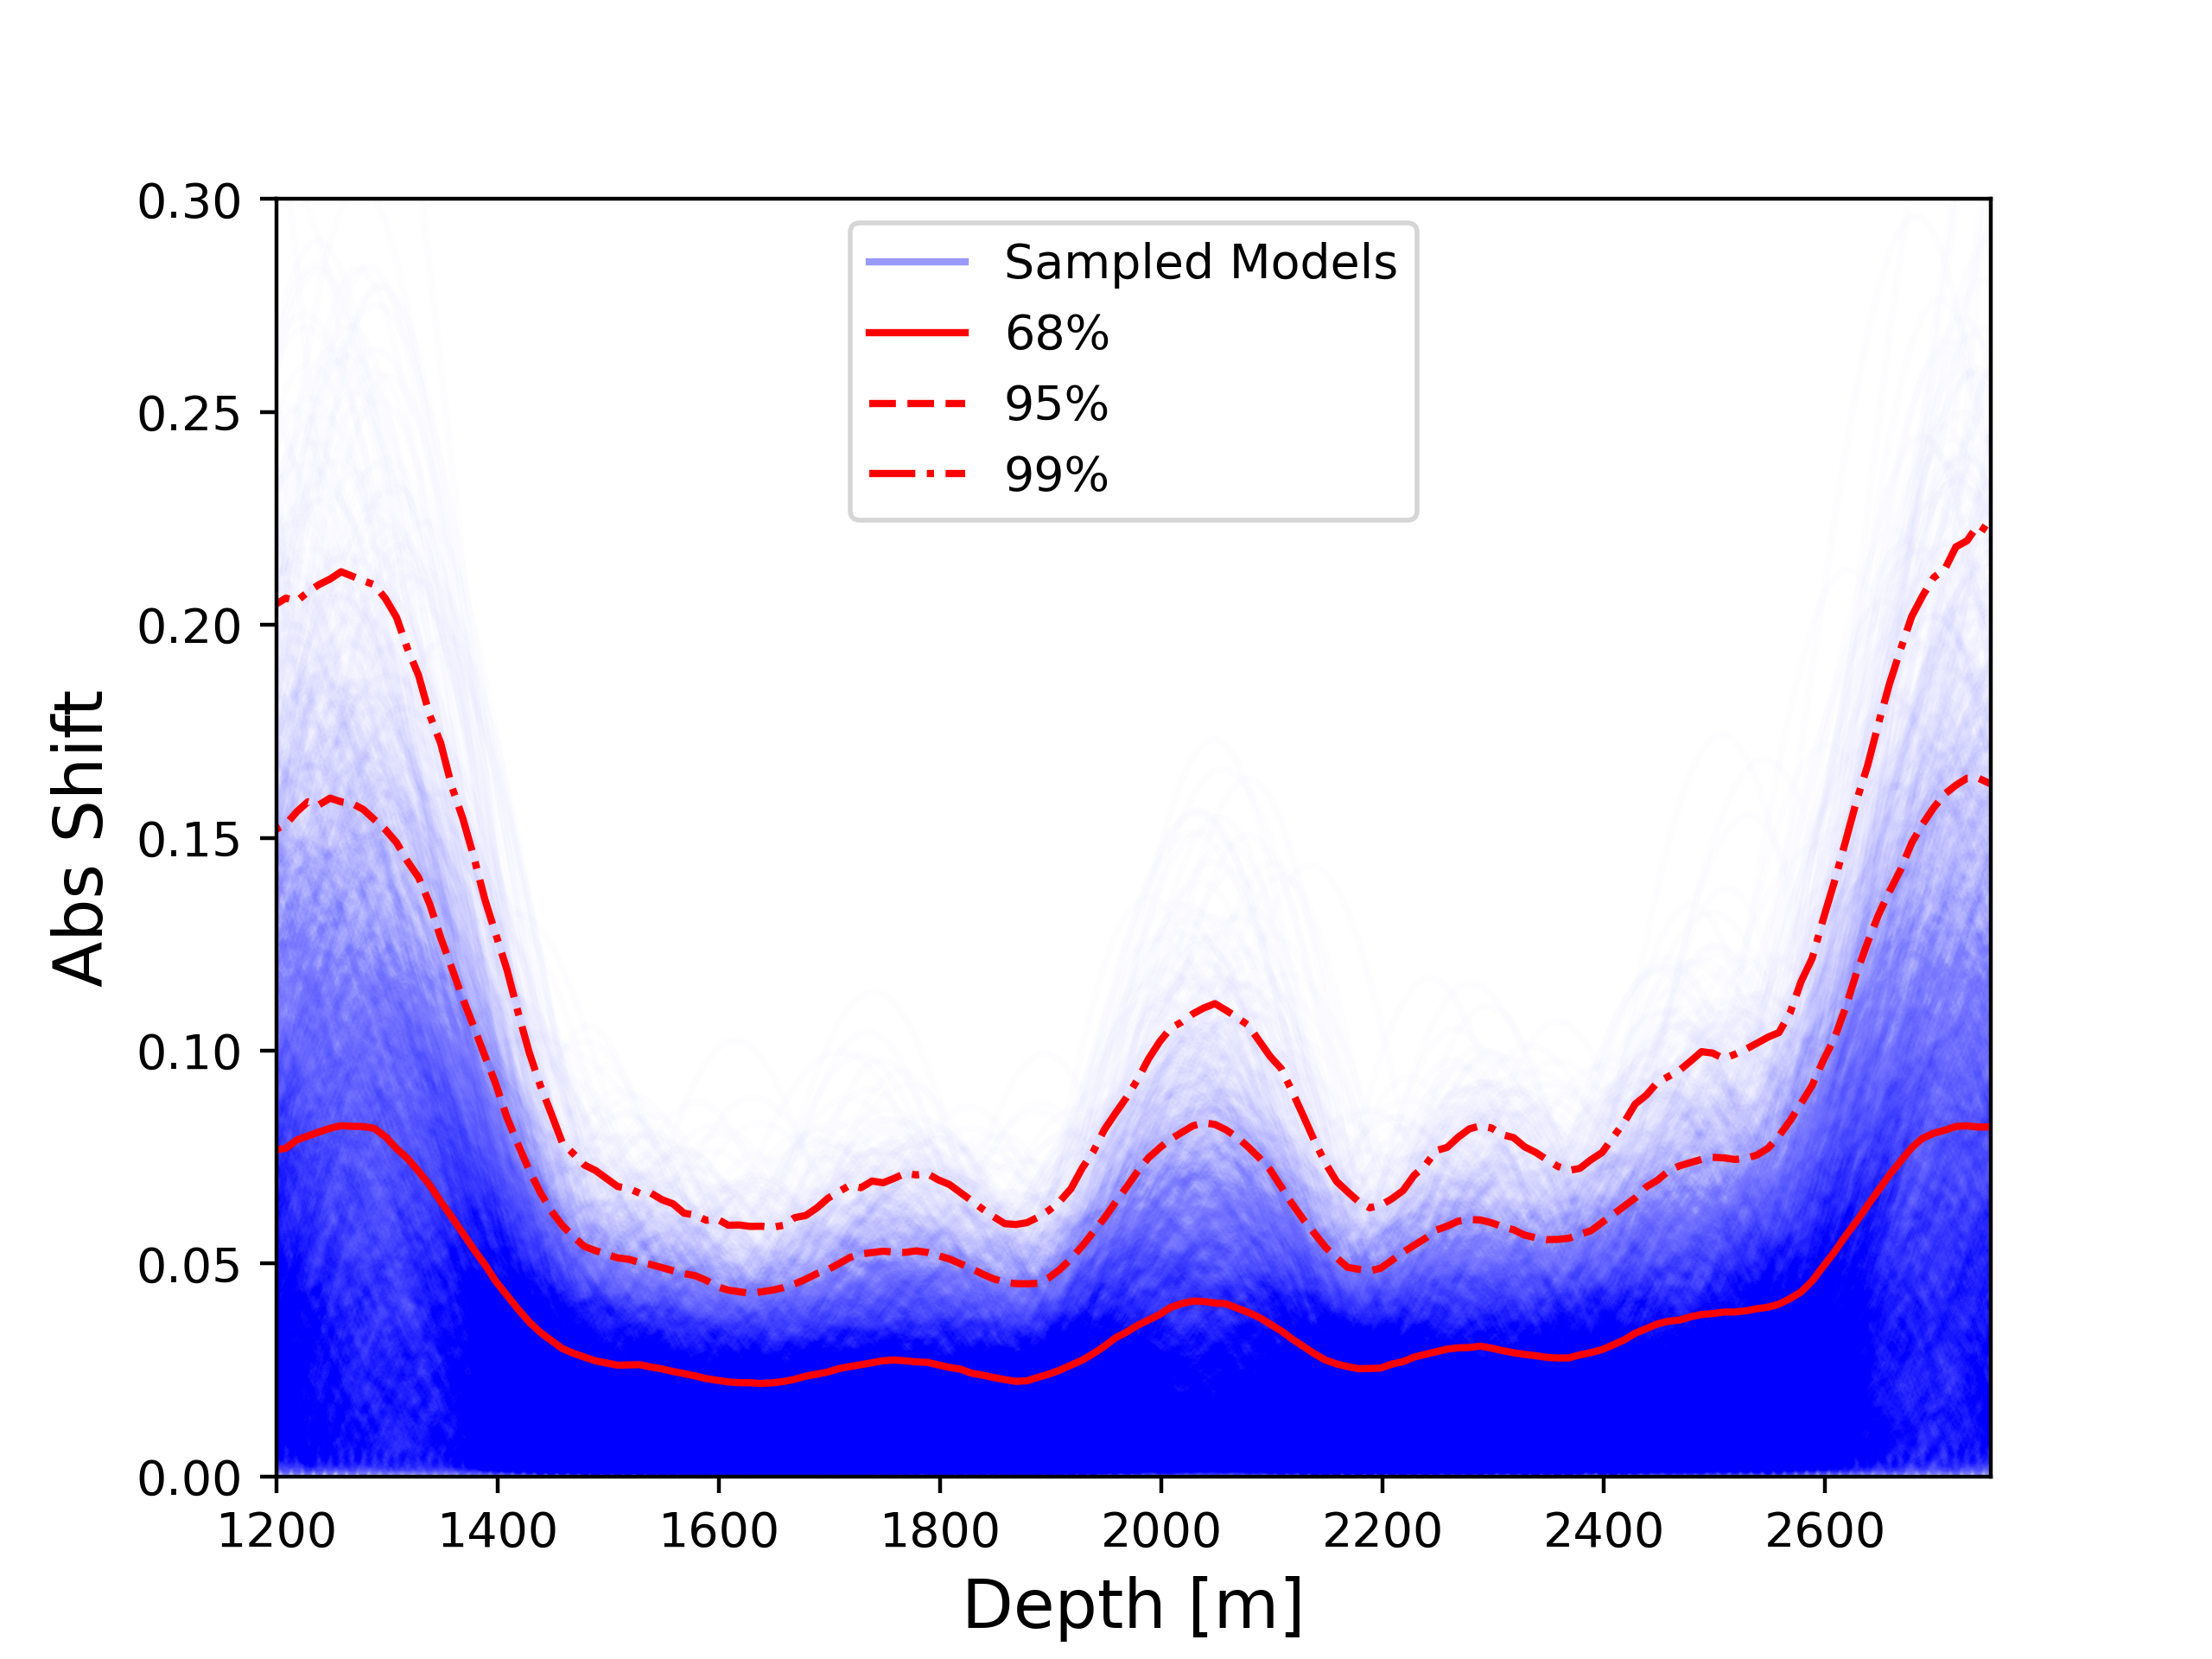
\includegraphics[width=0.8\linewidth]{figures/icemodel_smooth.png}
    \caption{The results of sampling five thousand ice models using the fit correlation matrix and widths for the amplitudes and phases. A solid red line is drawn, below which the fractional shift of the absorption length of 68\% of sampled models lie. Similar lines for 95\% and 99\%. IceCube lies between 1500 and 2500 meters of depth. The bump in the middle lines up with the dust layer in IceCube, and rises at the end are caused by poor constraint due to the physical extent of the detector.}\label{fig:envelope}
\end{figure}

The widths on the ice models were then used in an application of the SnowStorm technique. 
A purpose-build Monte Carlo sample was prepared generating only events that would yield cascades; since we were not interested in developing a sample to test event selection efficiency, background events were not included. 
This sample was generated using the same procedure as described in Chapter~\ref{chapter:gen}, starting with LeptonInjector for event generation and LeptonWeight for event weighting~\cite{ABBASI2021108018}. 
Energies were all sampled at according to a power law with a spectral index $\gamma=-2$.
Sub-samples were prepared spanning different energy regimes and using different numbers of events per file, injection cylinder sizes, and events per model. 
The full ensemble of event generation parameters are shown in Table~\ref{table:mc}.

\begin{table}
    \centering
    \rowcolors{2}{gray!25}{white}
    \begin{tabular}{c | ccc ccc ccc c}\rowcolor{blue!25}
            & 1001 & 1002 & 1003 & 1004 & 1005 & 1006 & 1007 & 1008 & 1009 & 1010 \\\hline
        
    Flavor  &$\nu_{e}$ &$\nu_{\mu}$ &$\nu_{\tau}$ &$\nu_{e}$ &$\nu_{\tau}$ &$\nu_{e}$ &$\nu_{\mu}$ &$\nu_{\tau}$ &$\nu_{e}$ &$\nu_{\tau}$  \\
    Current & NC & NC & NC & CC & CC & NC & NC & NC & CC & CC \\
    Events Per File & \multicolumn{5}{c}{50,000} & \multicolumn{5}{c}{10,000} \\
    $E_{min}$ [GeV] & \multicolumn{5}{c}{100} & \multicolumn{5}{c}{$5e3$} \\
    $E_{max}$ [GeV] & \multicolumn{5}{c}{$5e3$} & \multicolumn{5}{c}{$10e6$}\\
    Zenith Range & \multicolumn{10}{c}{Full Sky}\\
    Cylinder Height & \multicolumn{10}{c}{1400 m}\\
    Cylinder Radius & \multicolumn{5}{c}{700 m} & \multicolumn{5}{c}{750 m} \\
    Sampled $\gamma$ & \multicolumn{10}{c}{-2} \\
    Events Per Model & \multicolumn{5}{c}{5} & \multicolumn{5}{c}{10} 
    \end{tabular}
    \caption{MC generation specifications for the snowstorm cascades sample. Cylinder height and radius are defined in Ref~\cite{ABBASI2021108018}. The number of events per model refers to the number of MC events simulated before shuffling the amplitudes and phases for the ice model.}\label{table:mc}
\end{table}

From these, splits were applied to the full sample and 2D linear gradients were calculated. 
Photospline~\cite{WHITEHORN20132214} was then used to perform spline fits of the 2D gradients to smooth out MC statistical variance. 
A table of spline fits is shown below in Figure~\ref{fig:gradients}. 

\begin{figure}
    \centering
    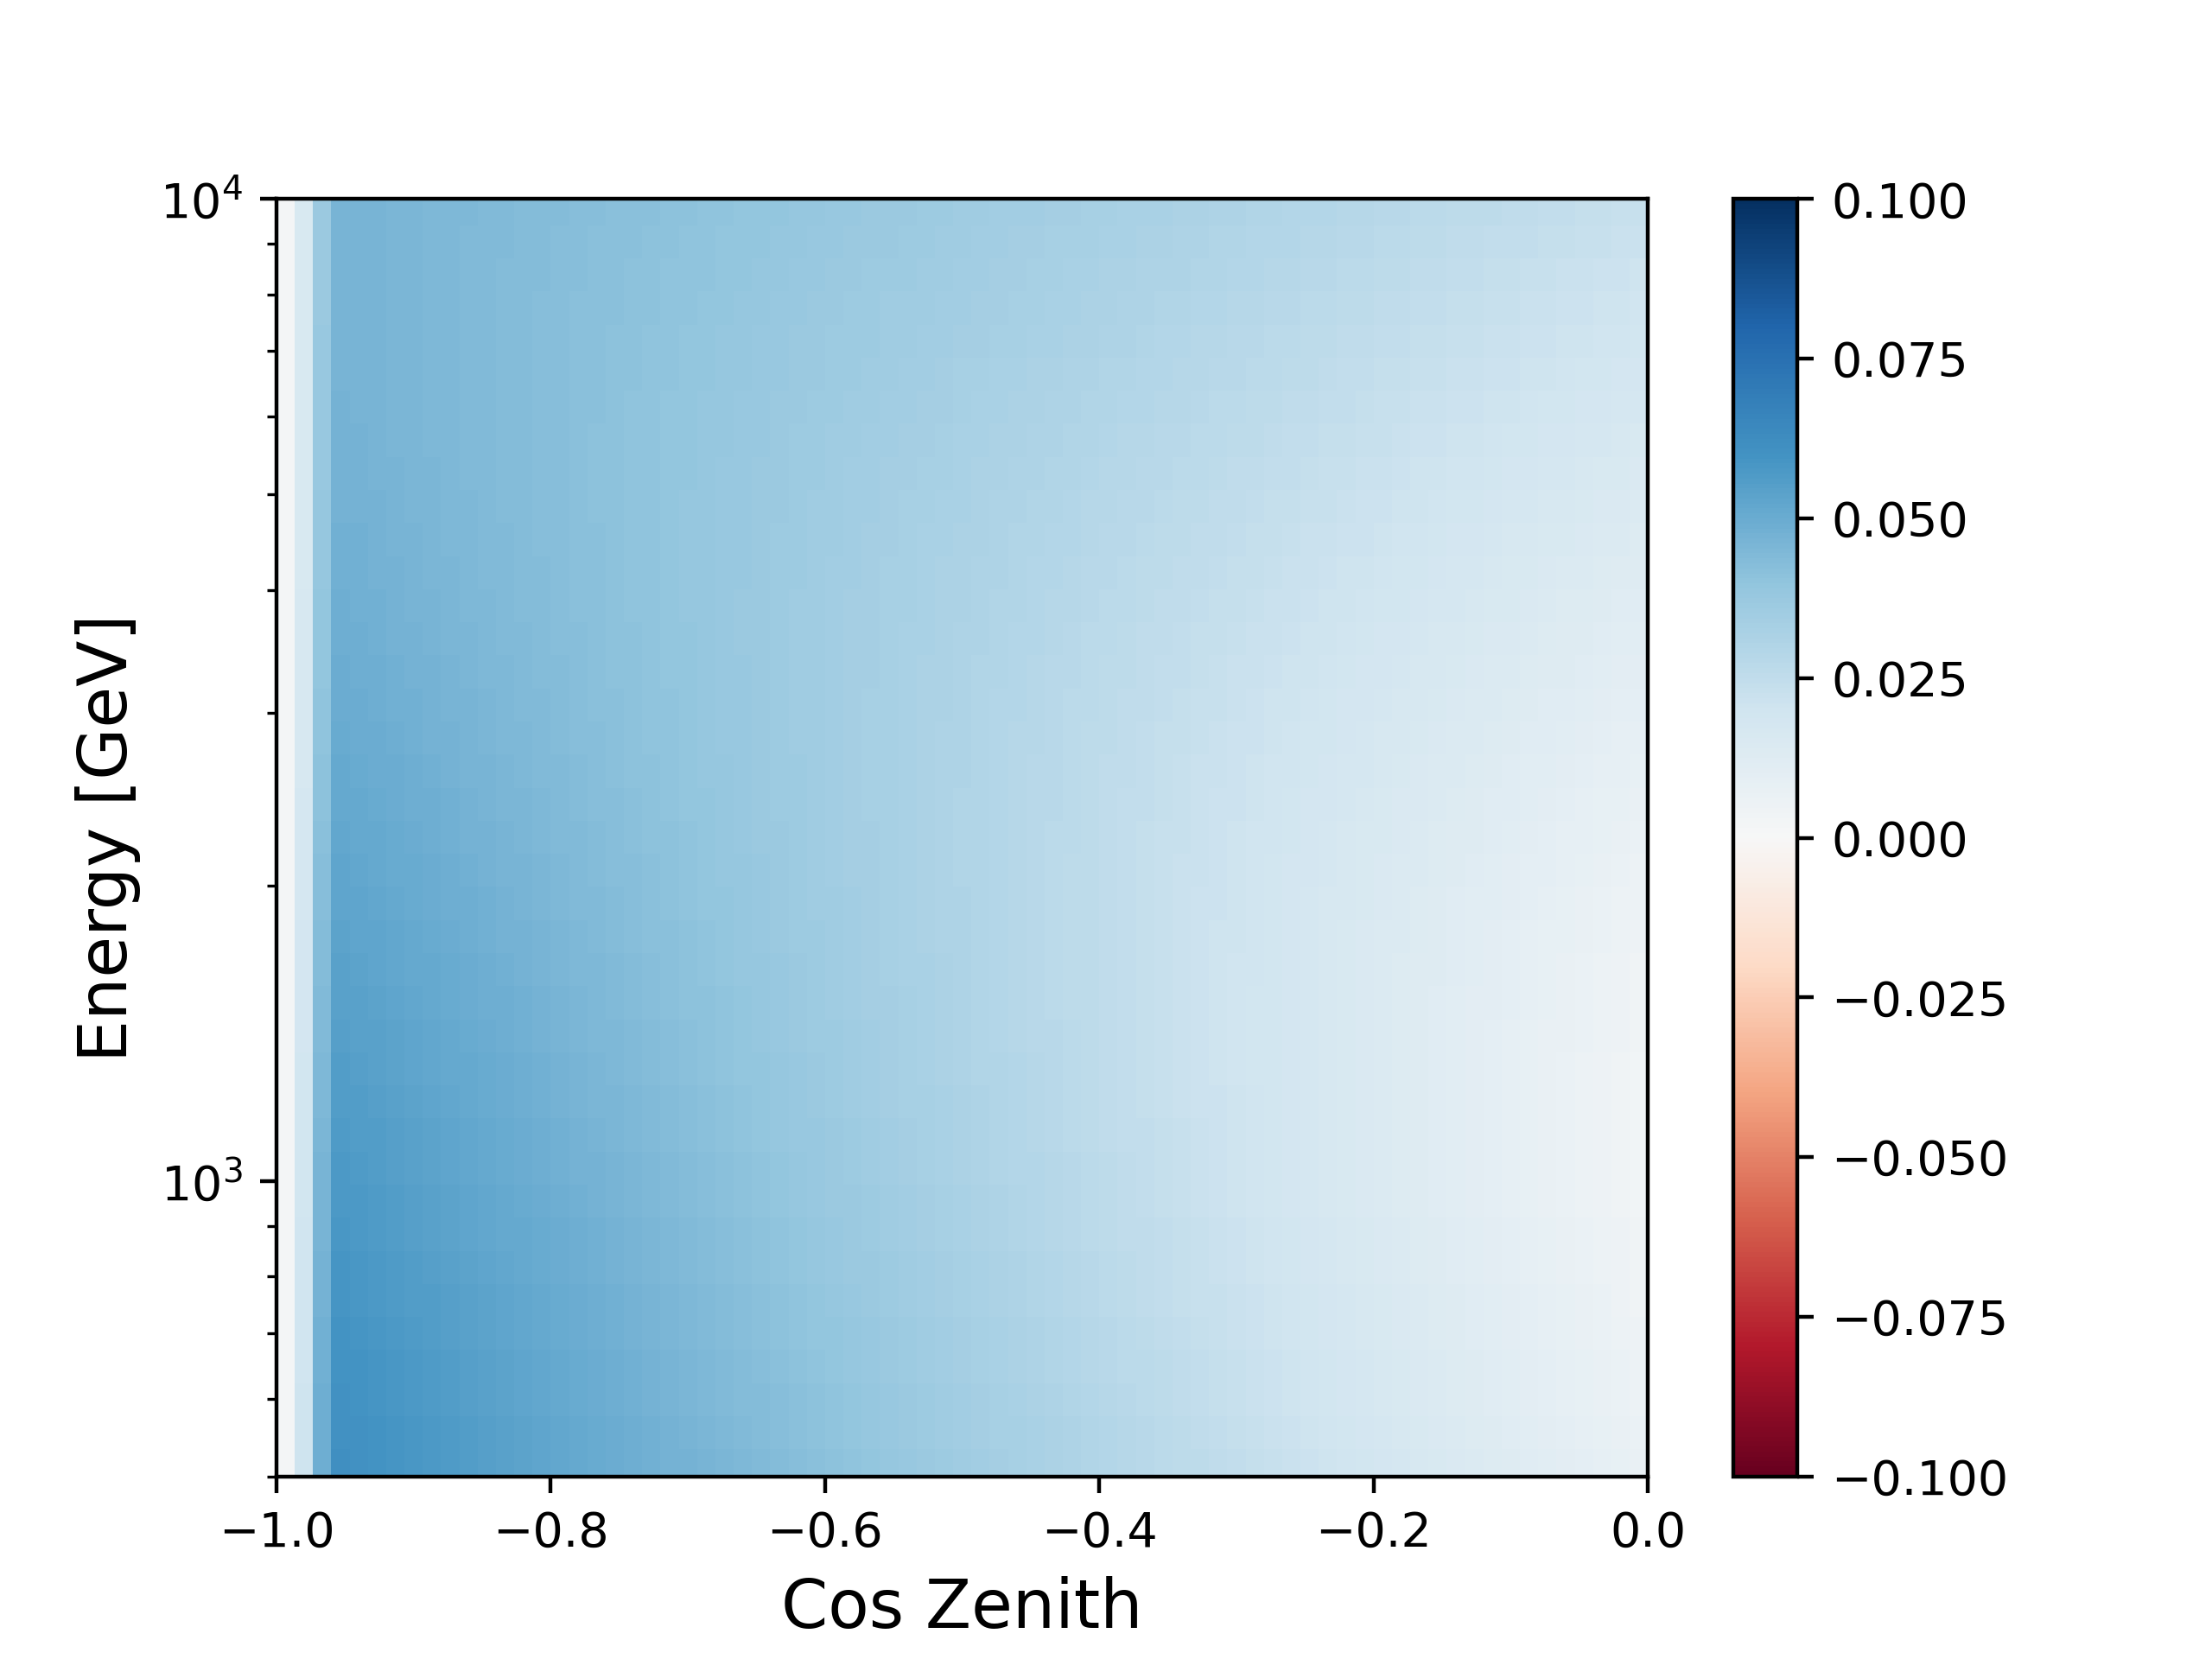
\includegraphics[width=0.3\linewidth]{figures/spline_amp00_gradient.png}%
    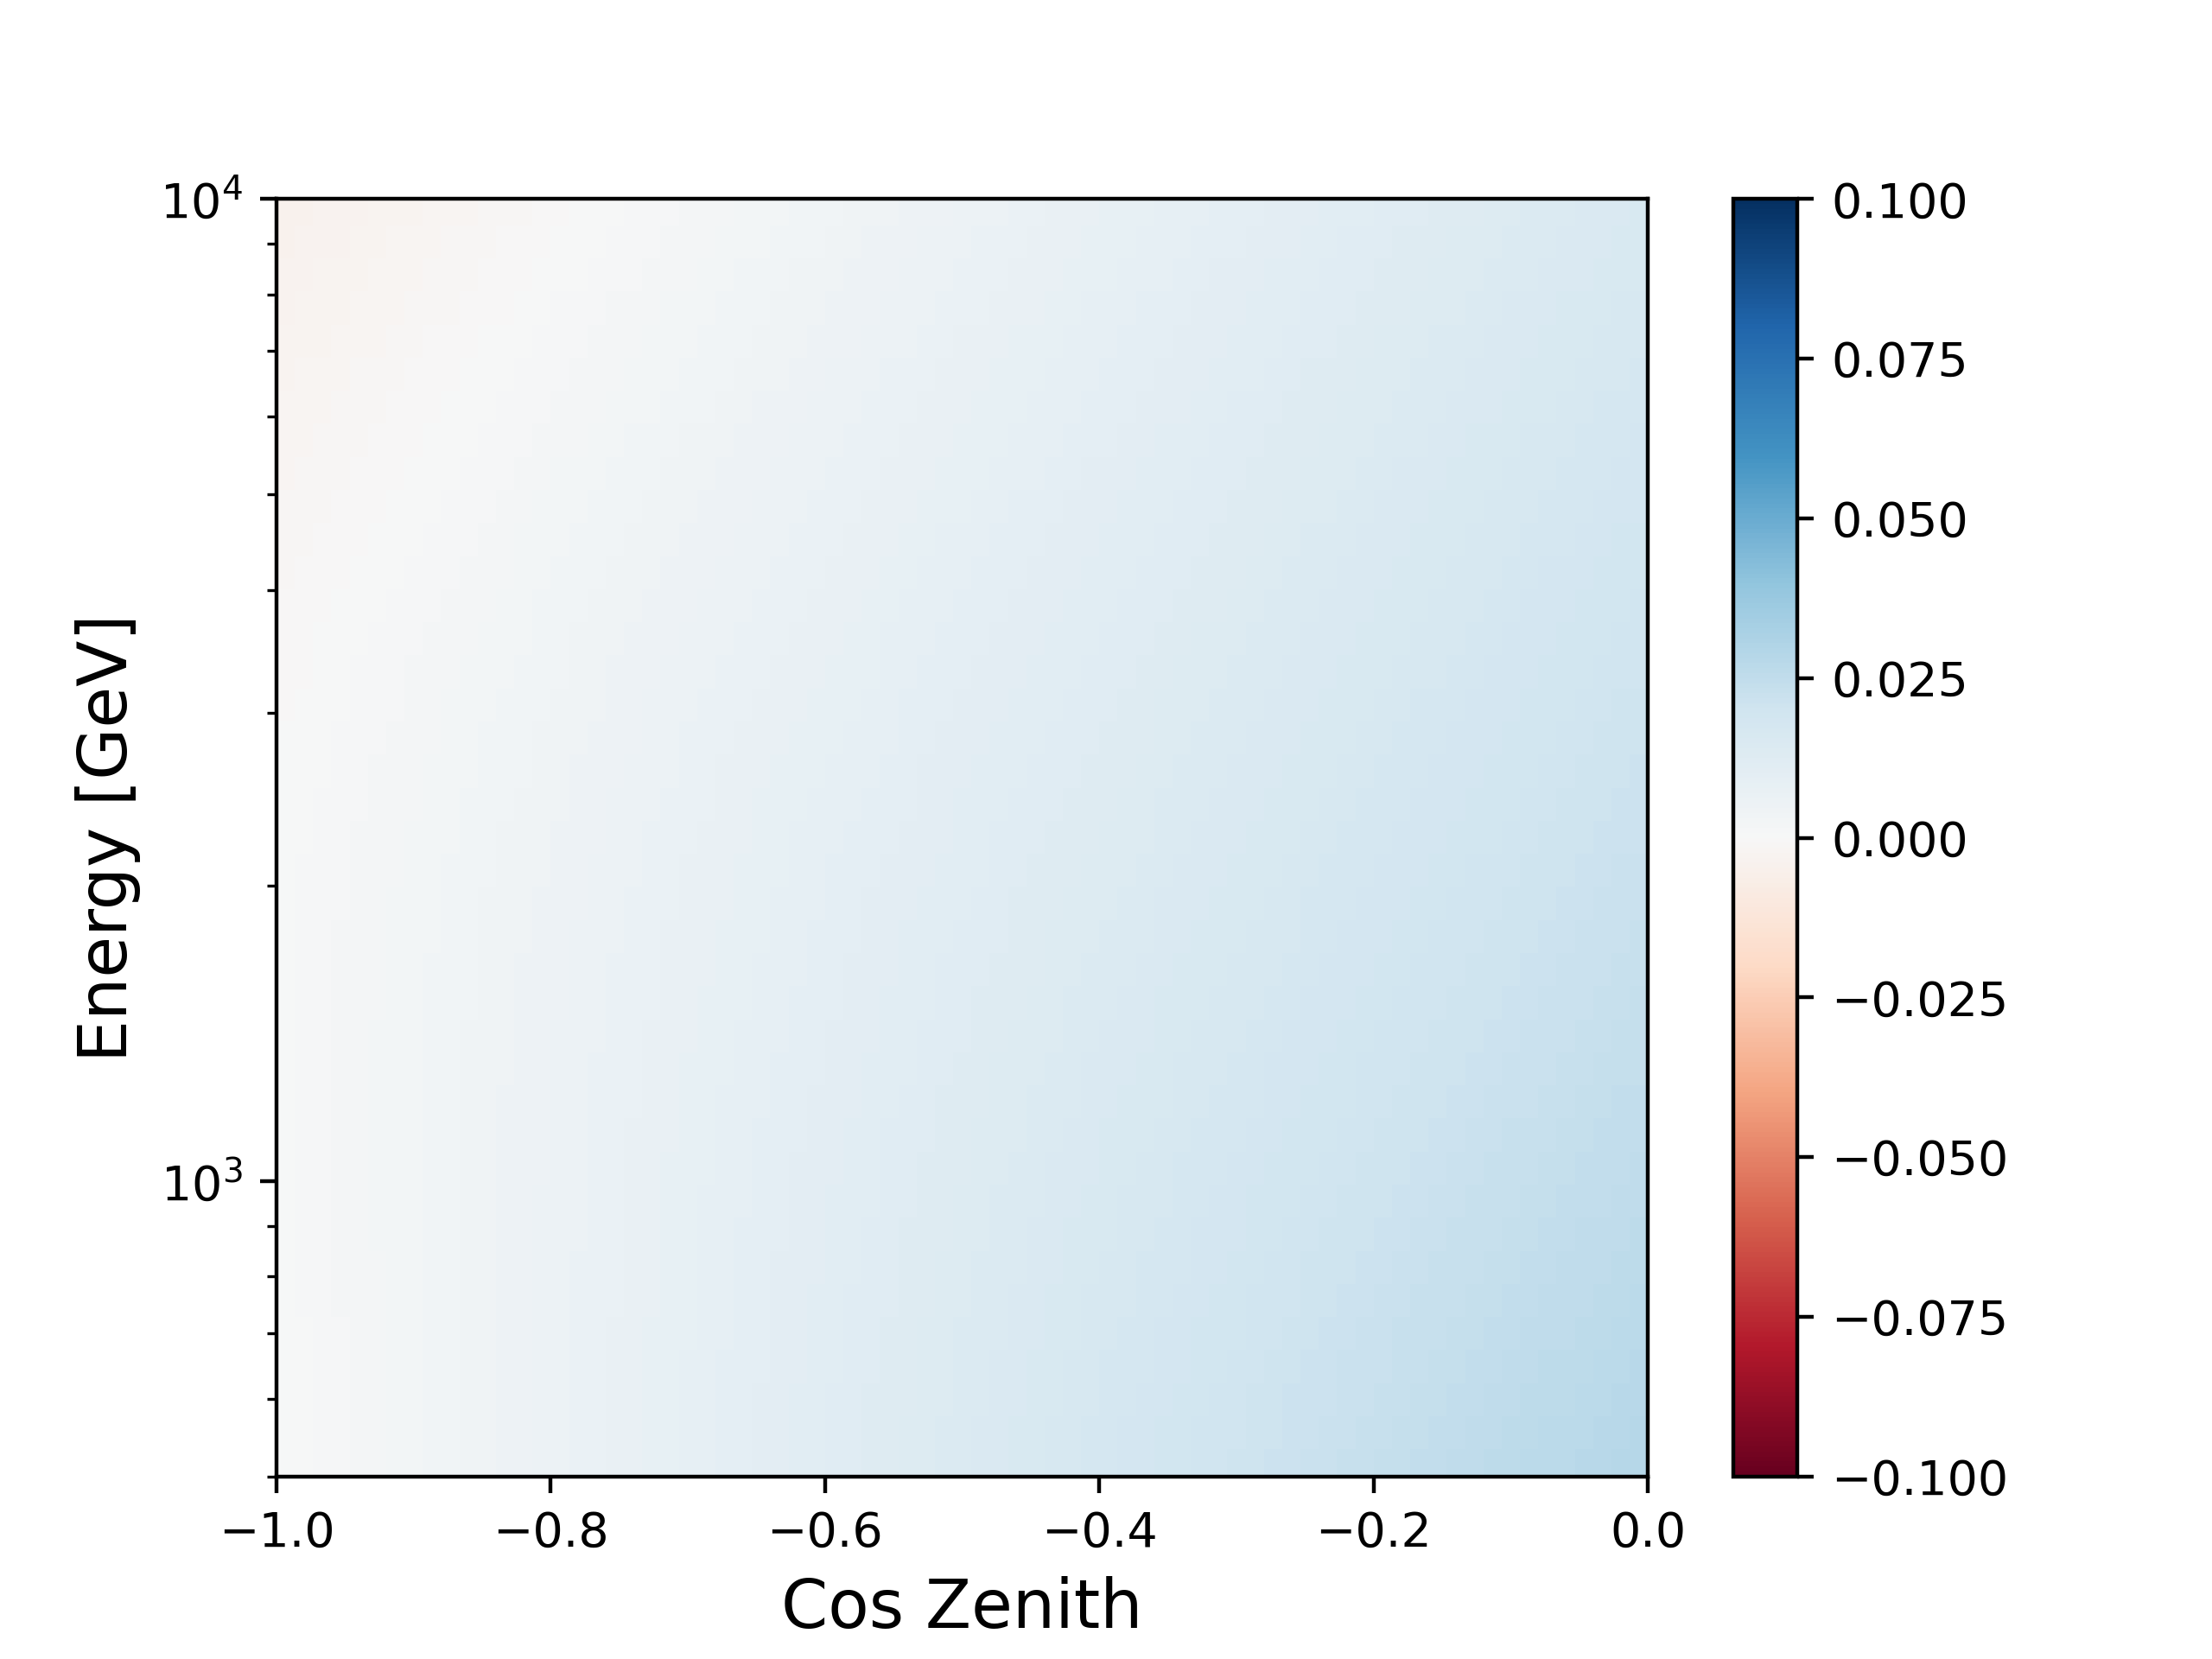
\includegraphics[width=0.3\linewidth]{figures/spline_amp01_gradient.png}%
    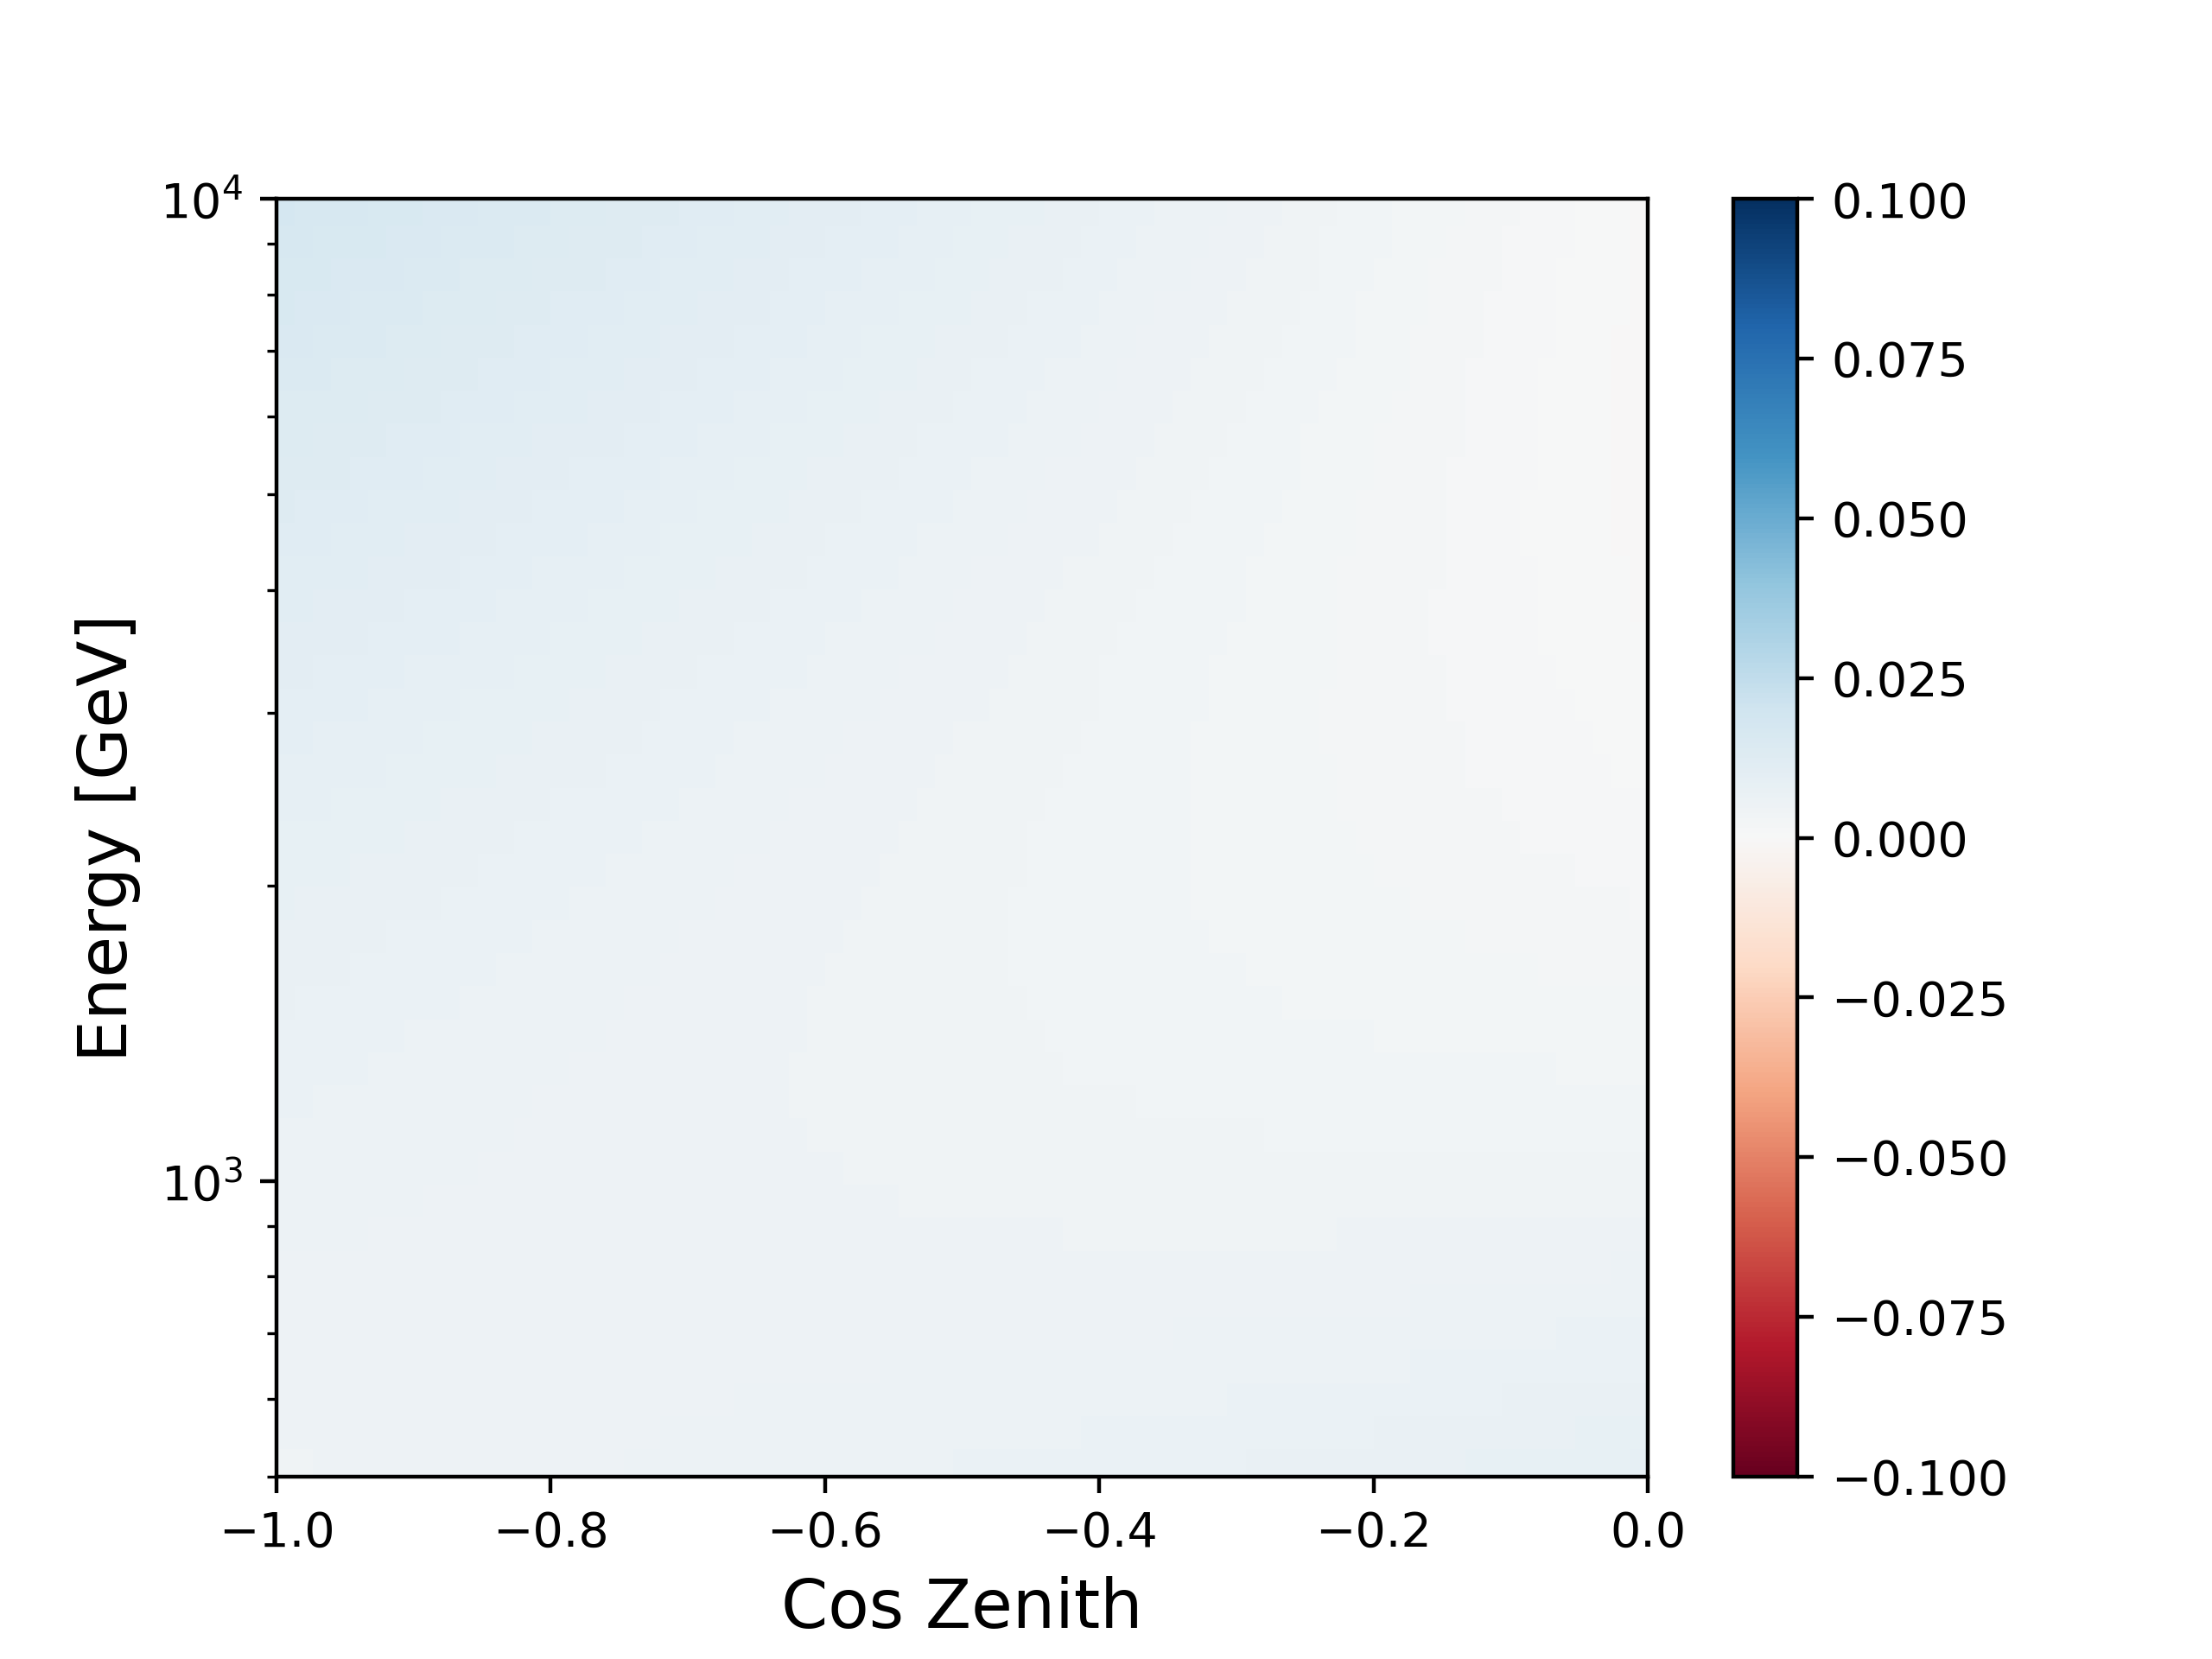
\includegraphics[width=0.3\linewidth]{figures/spline_amp02_gradient.png}\\
    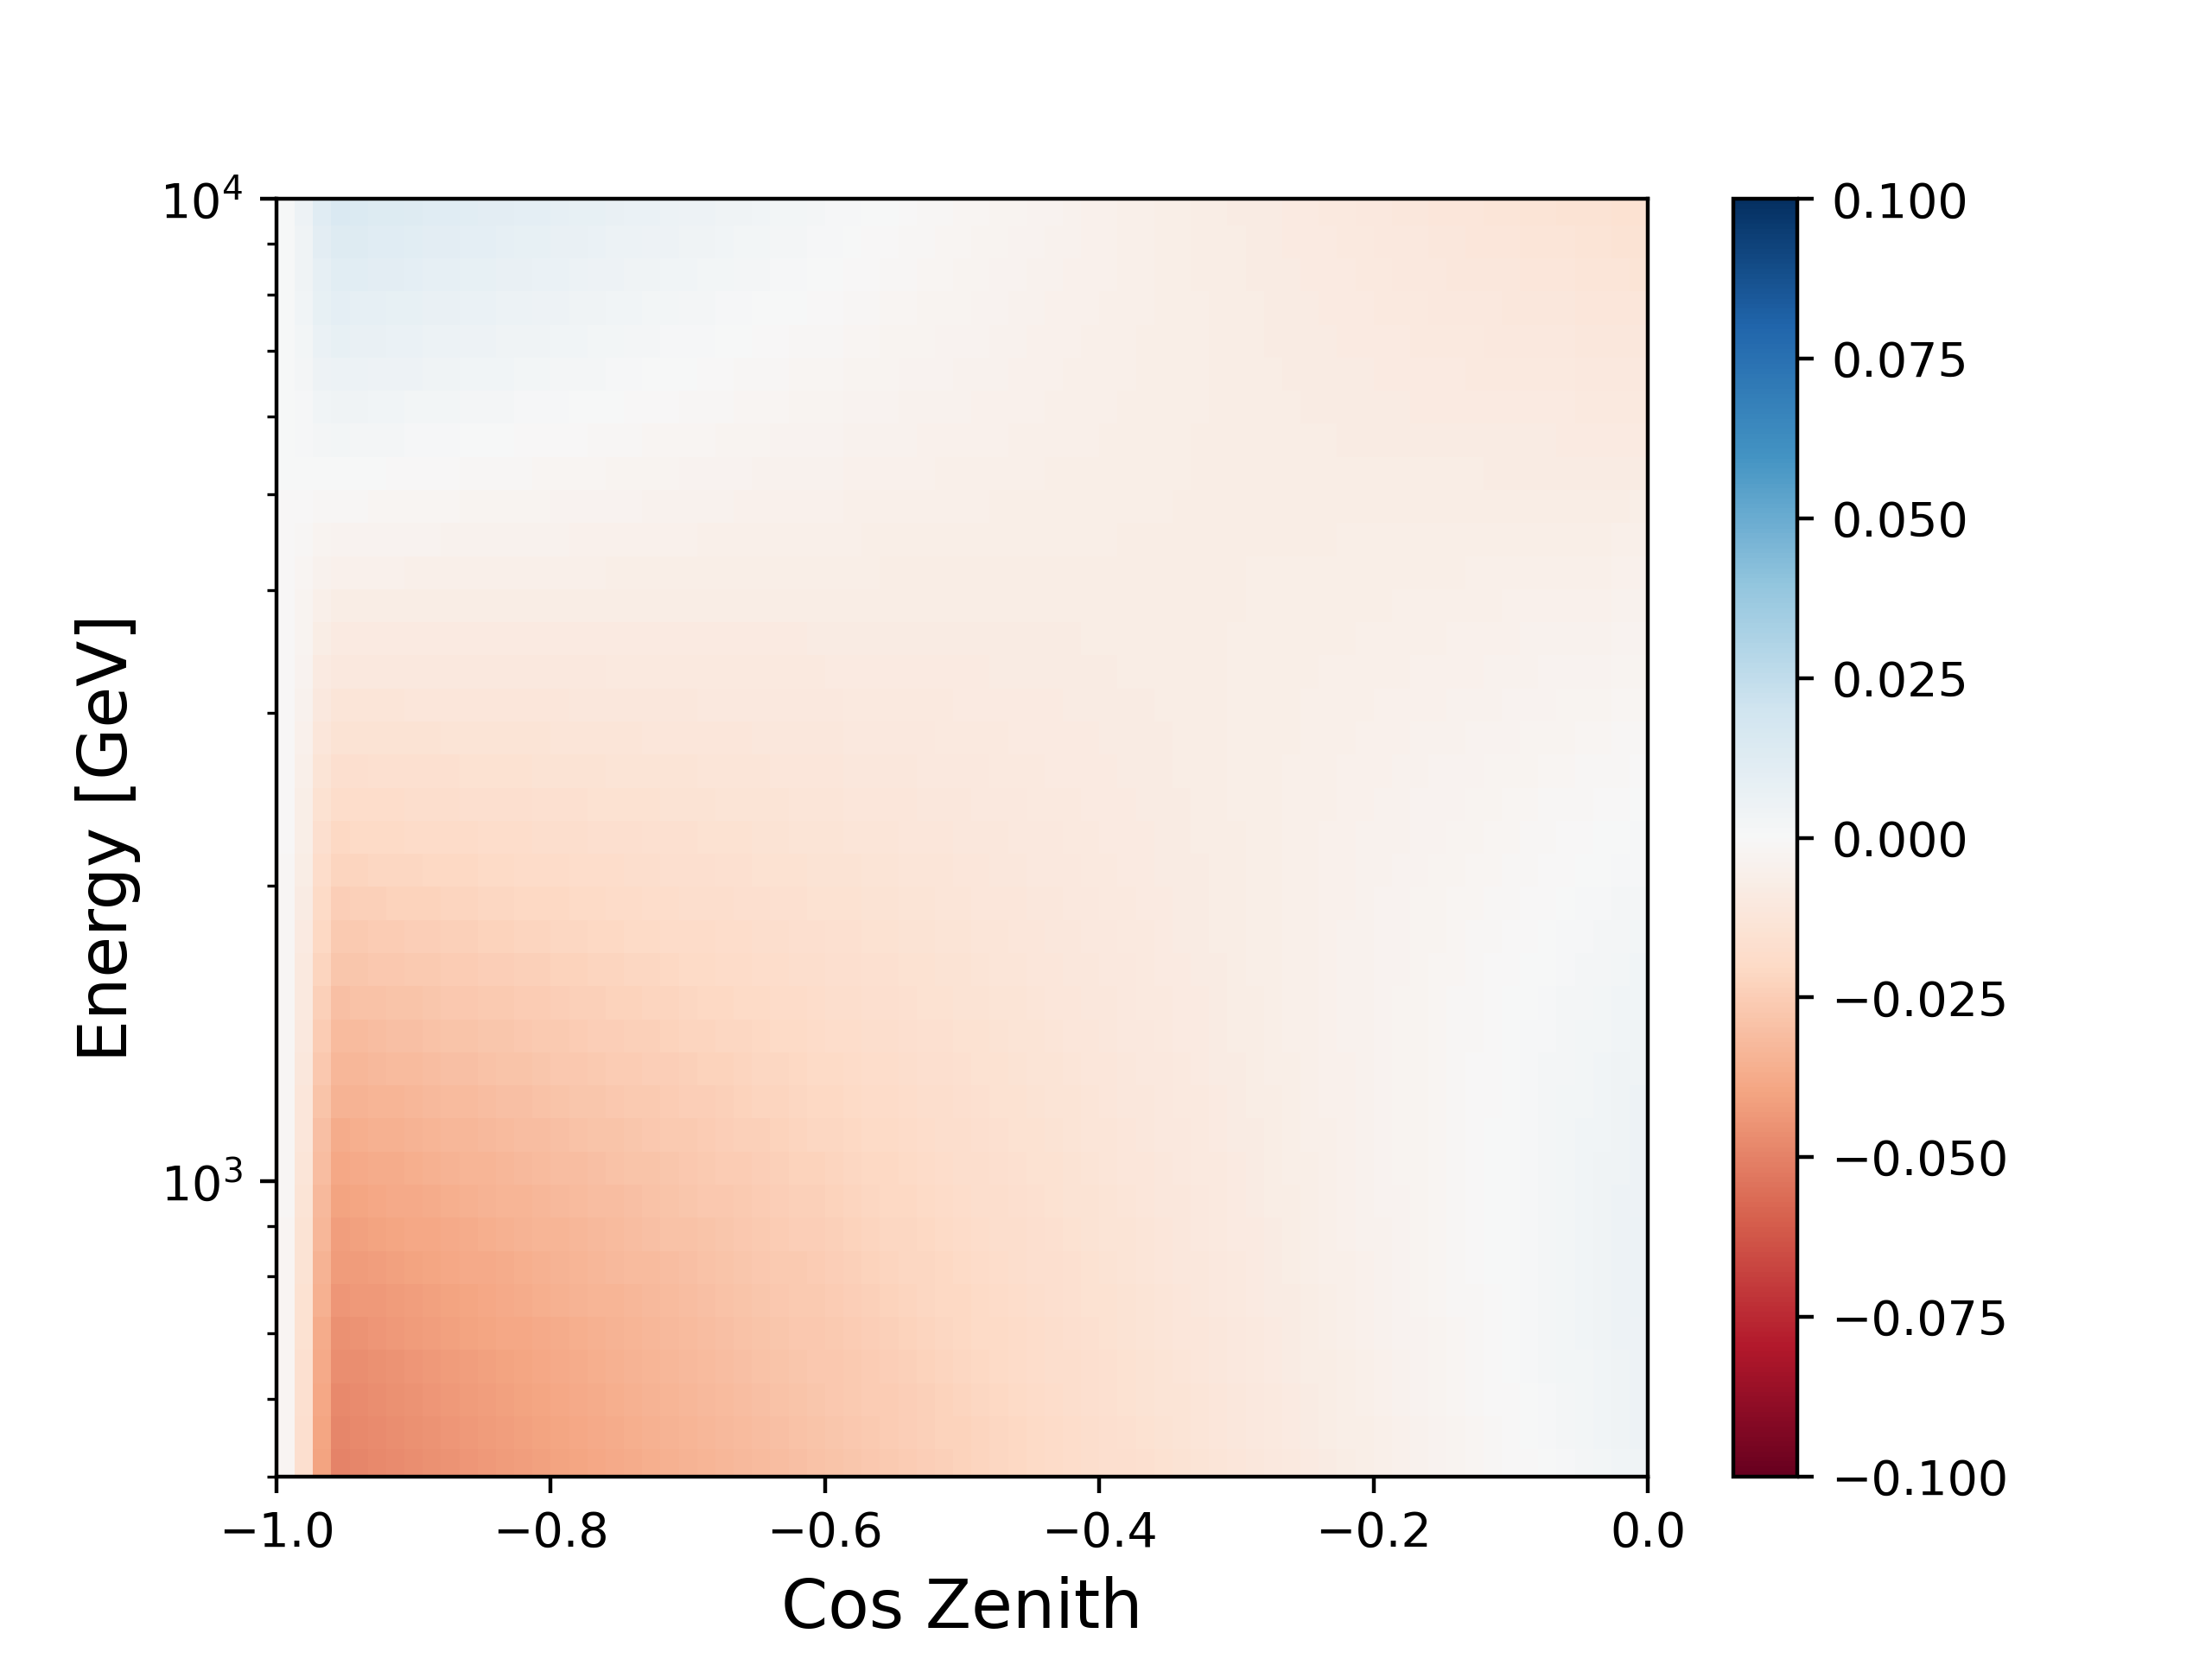
\includegraphics[width=0.3\linewidth]{figures/spline_amp03_gradient.png}%
    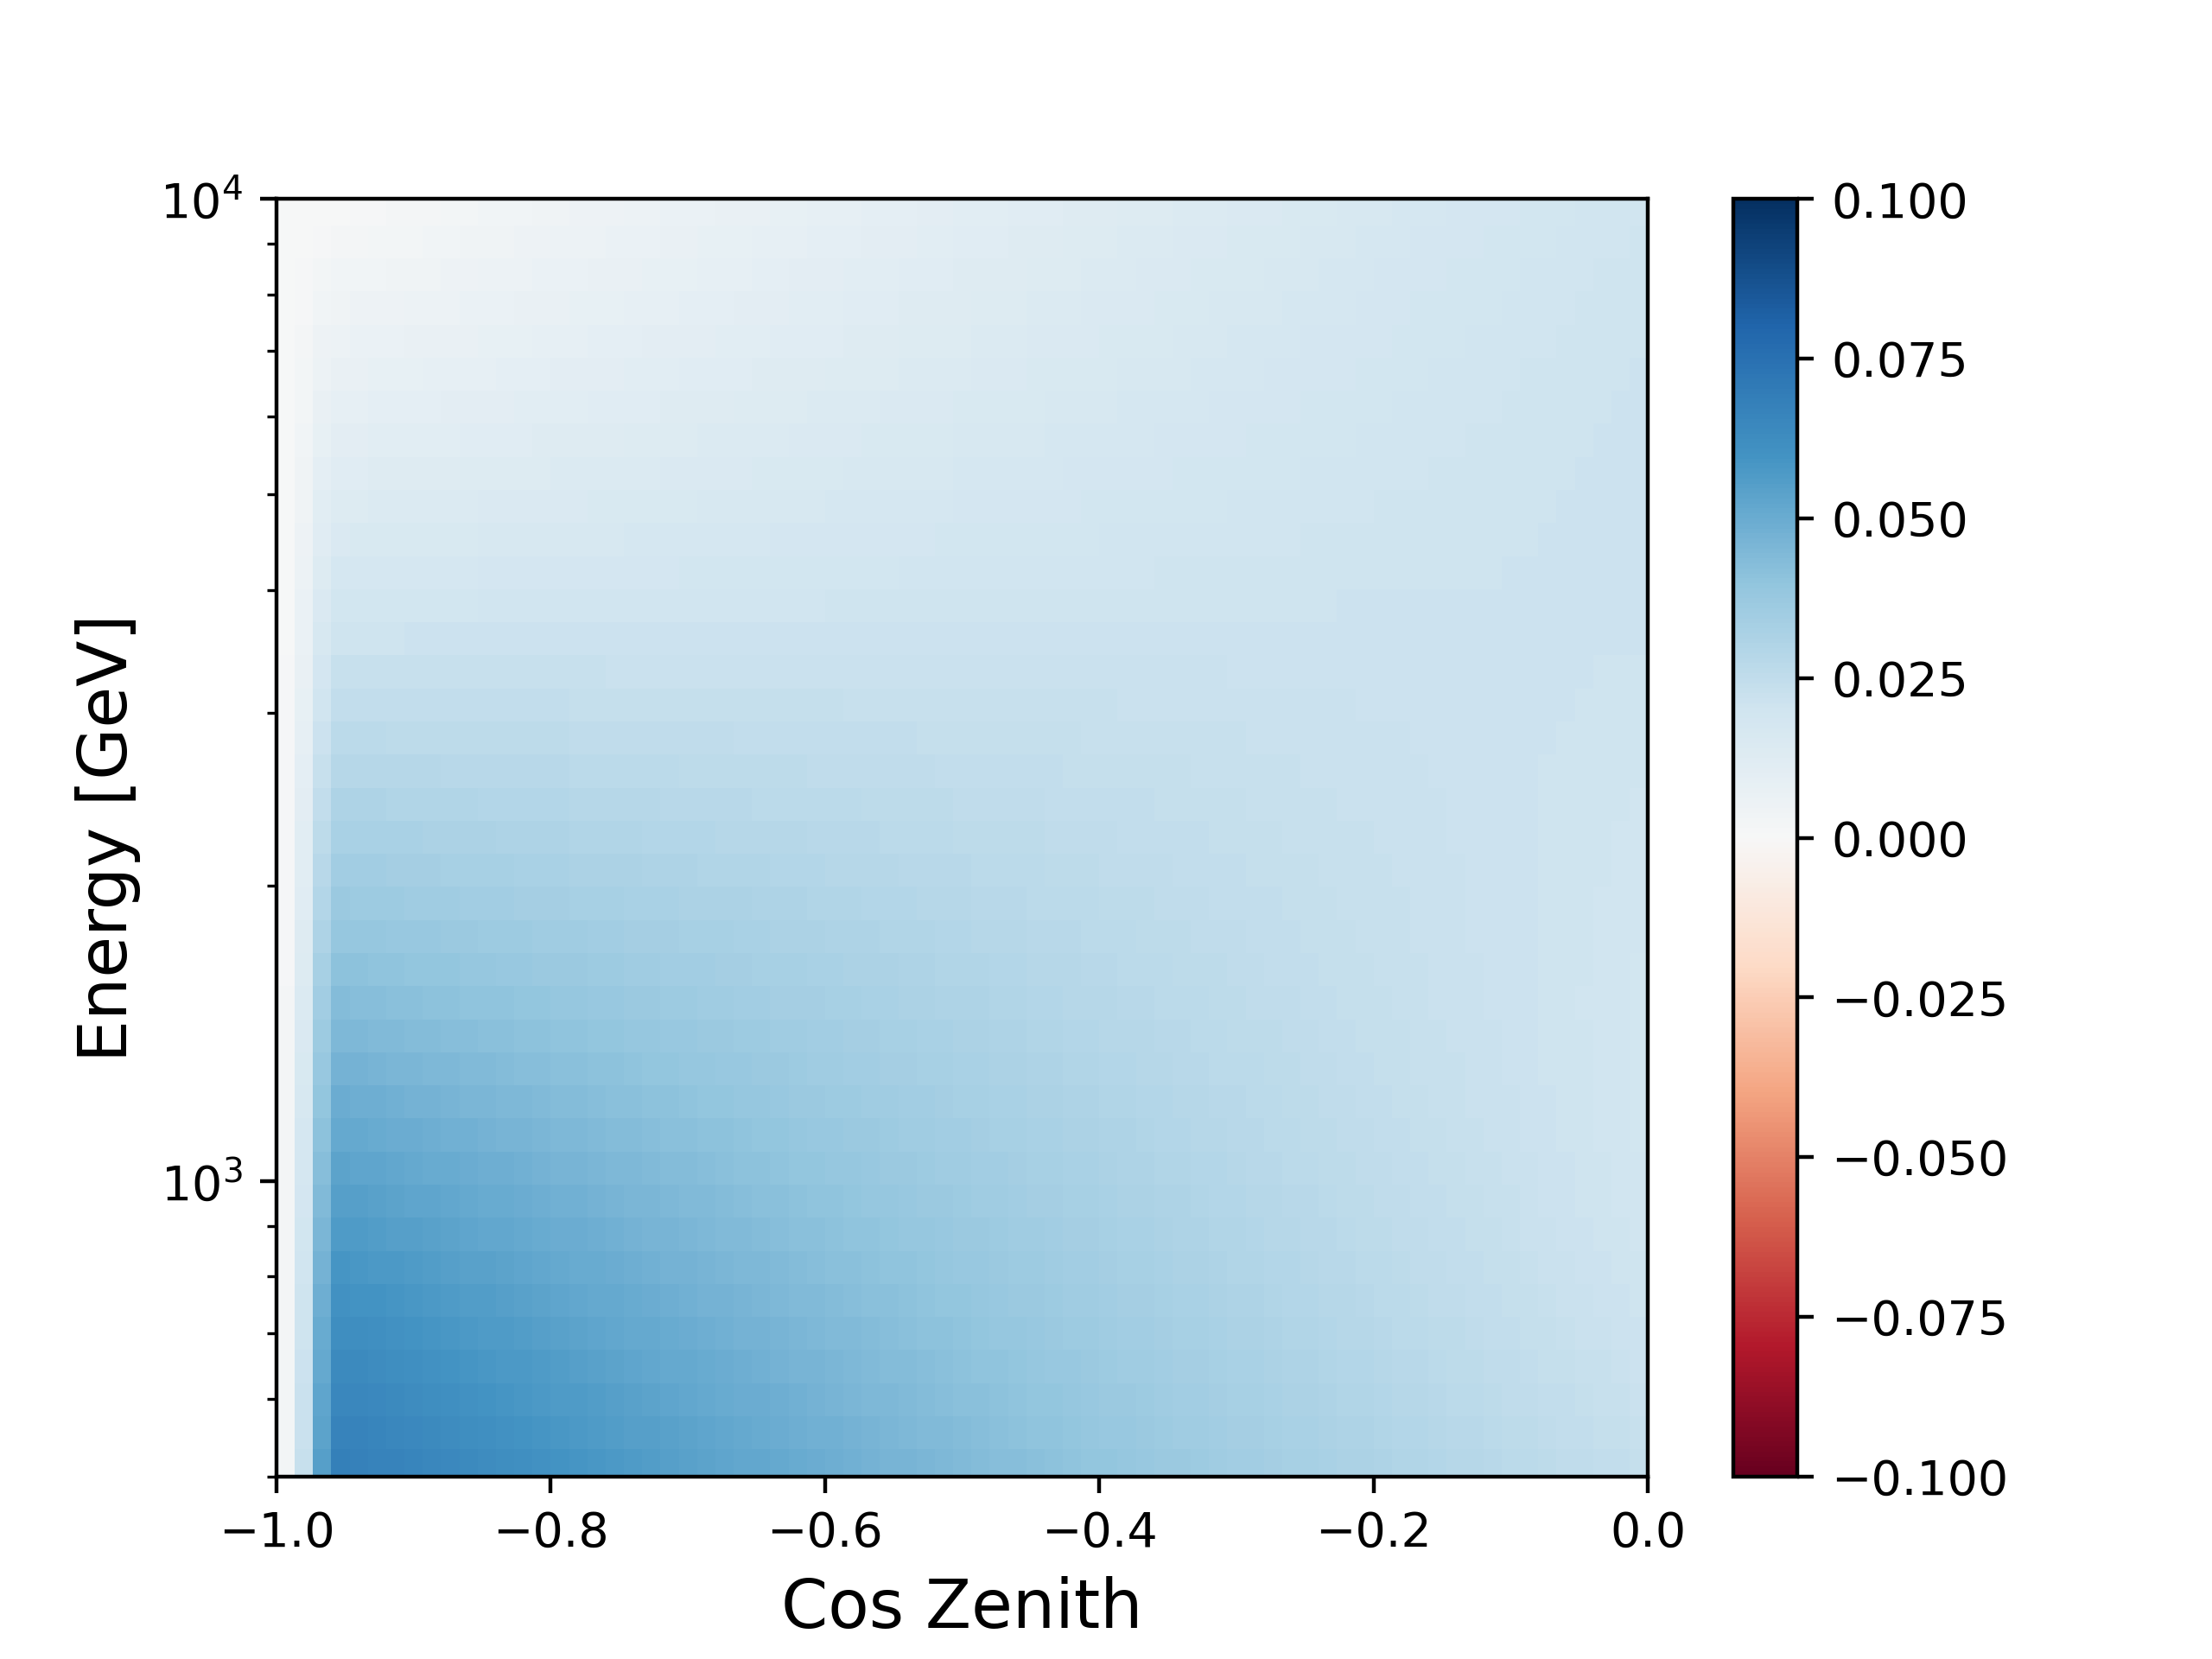
\includegraphics[width=0.3\linewidth]{figures/spline_amp04_gradient.png}%
    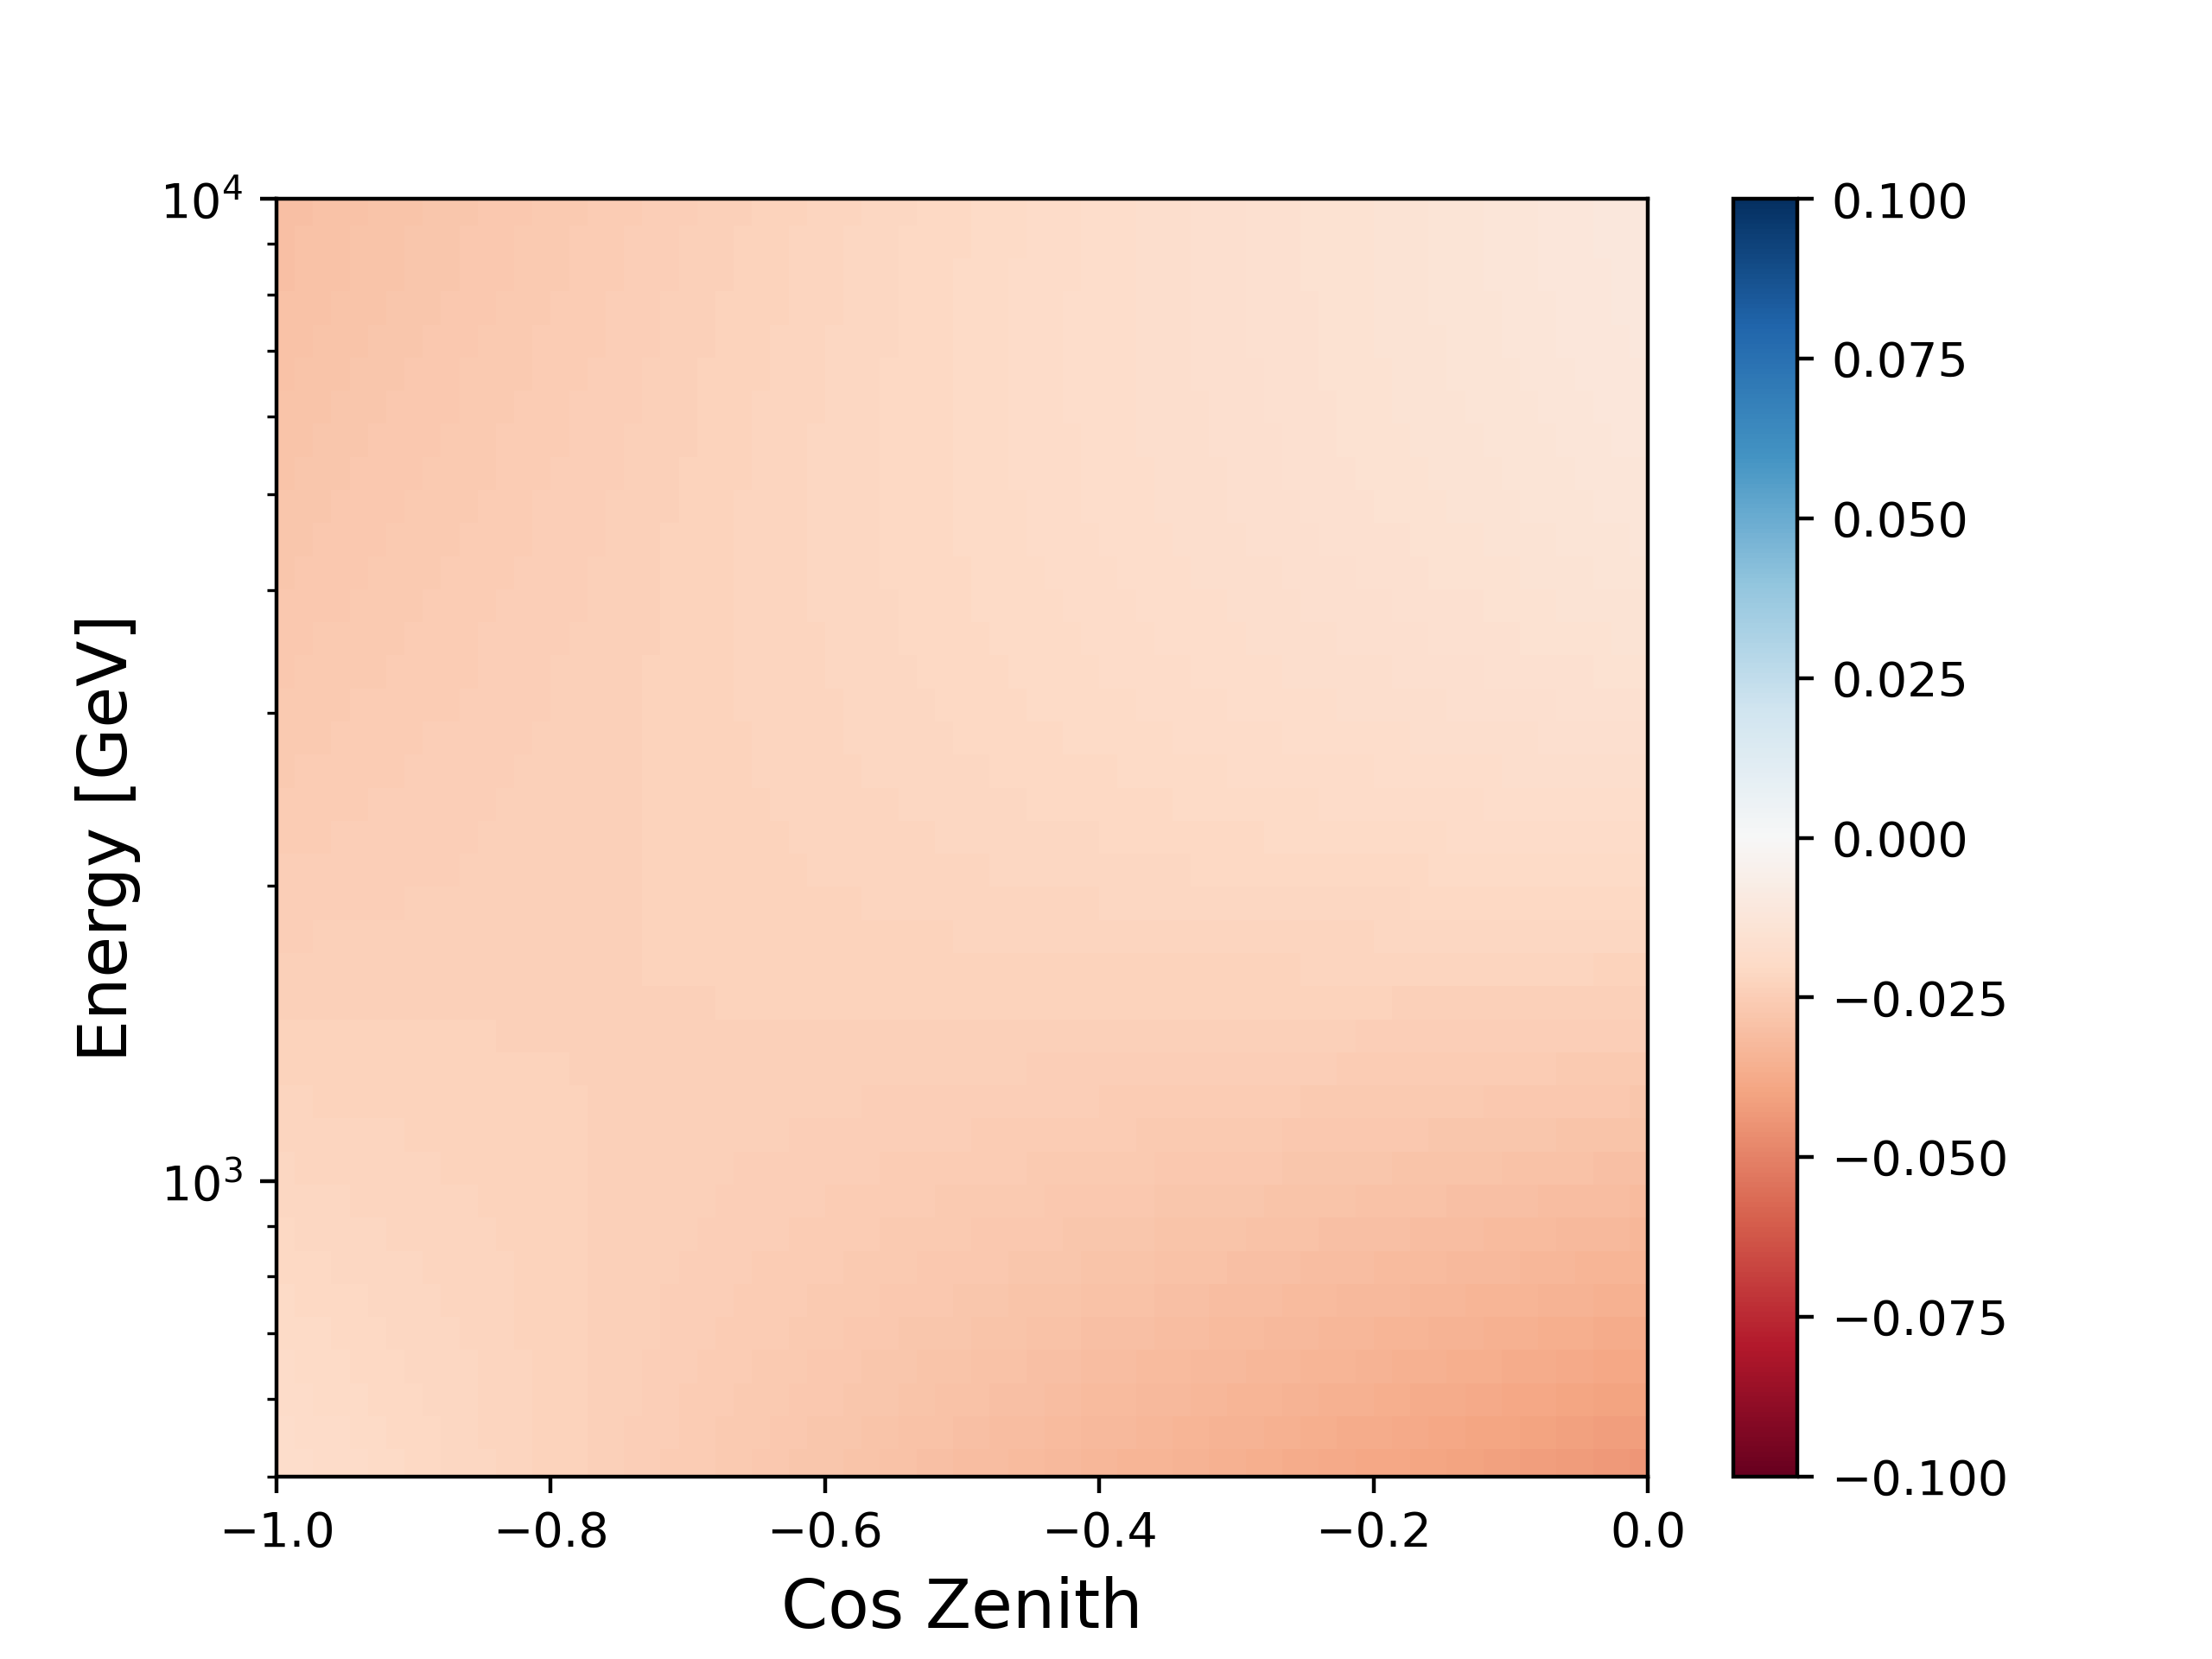
\includegraphics[width=0.3\linewidth]{figures/spline_phase01_gradient.png}\\
    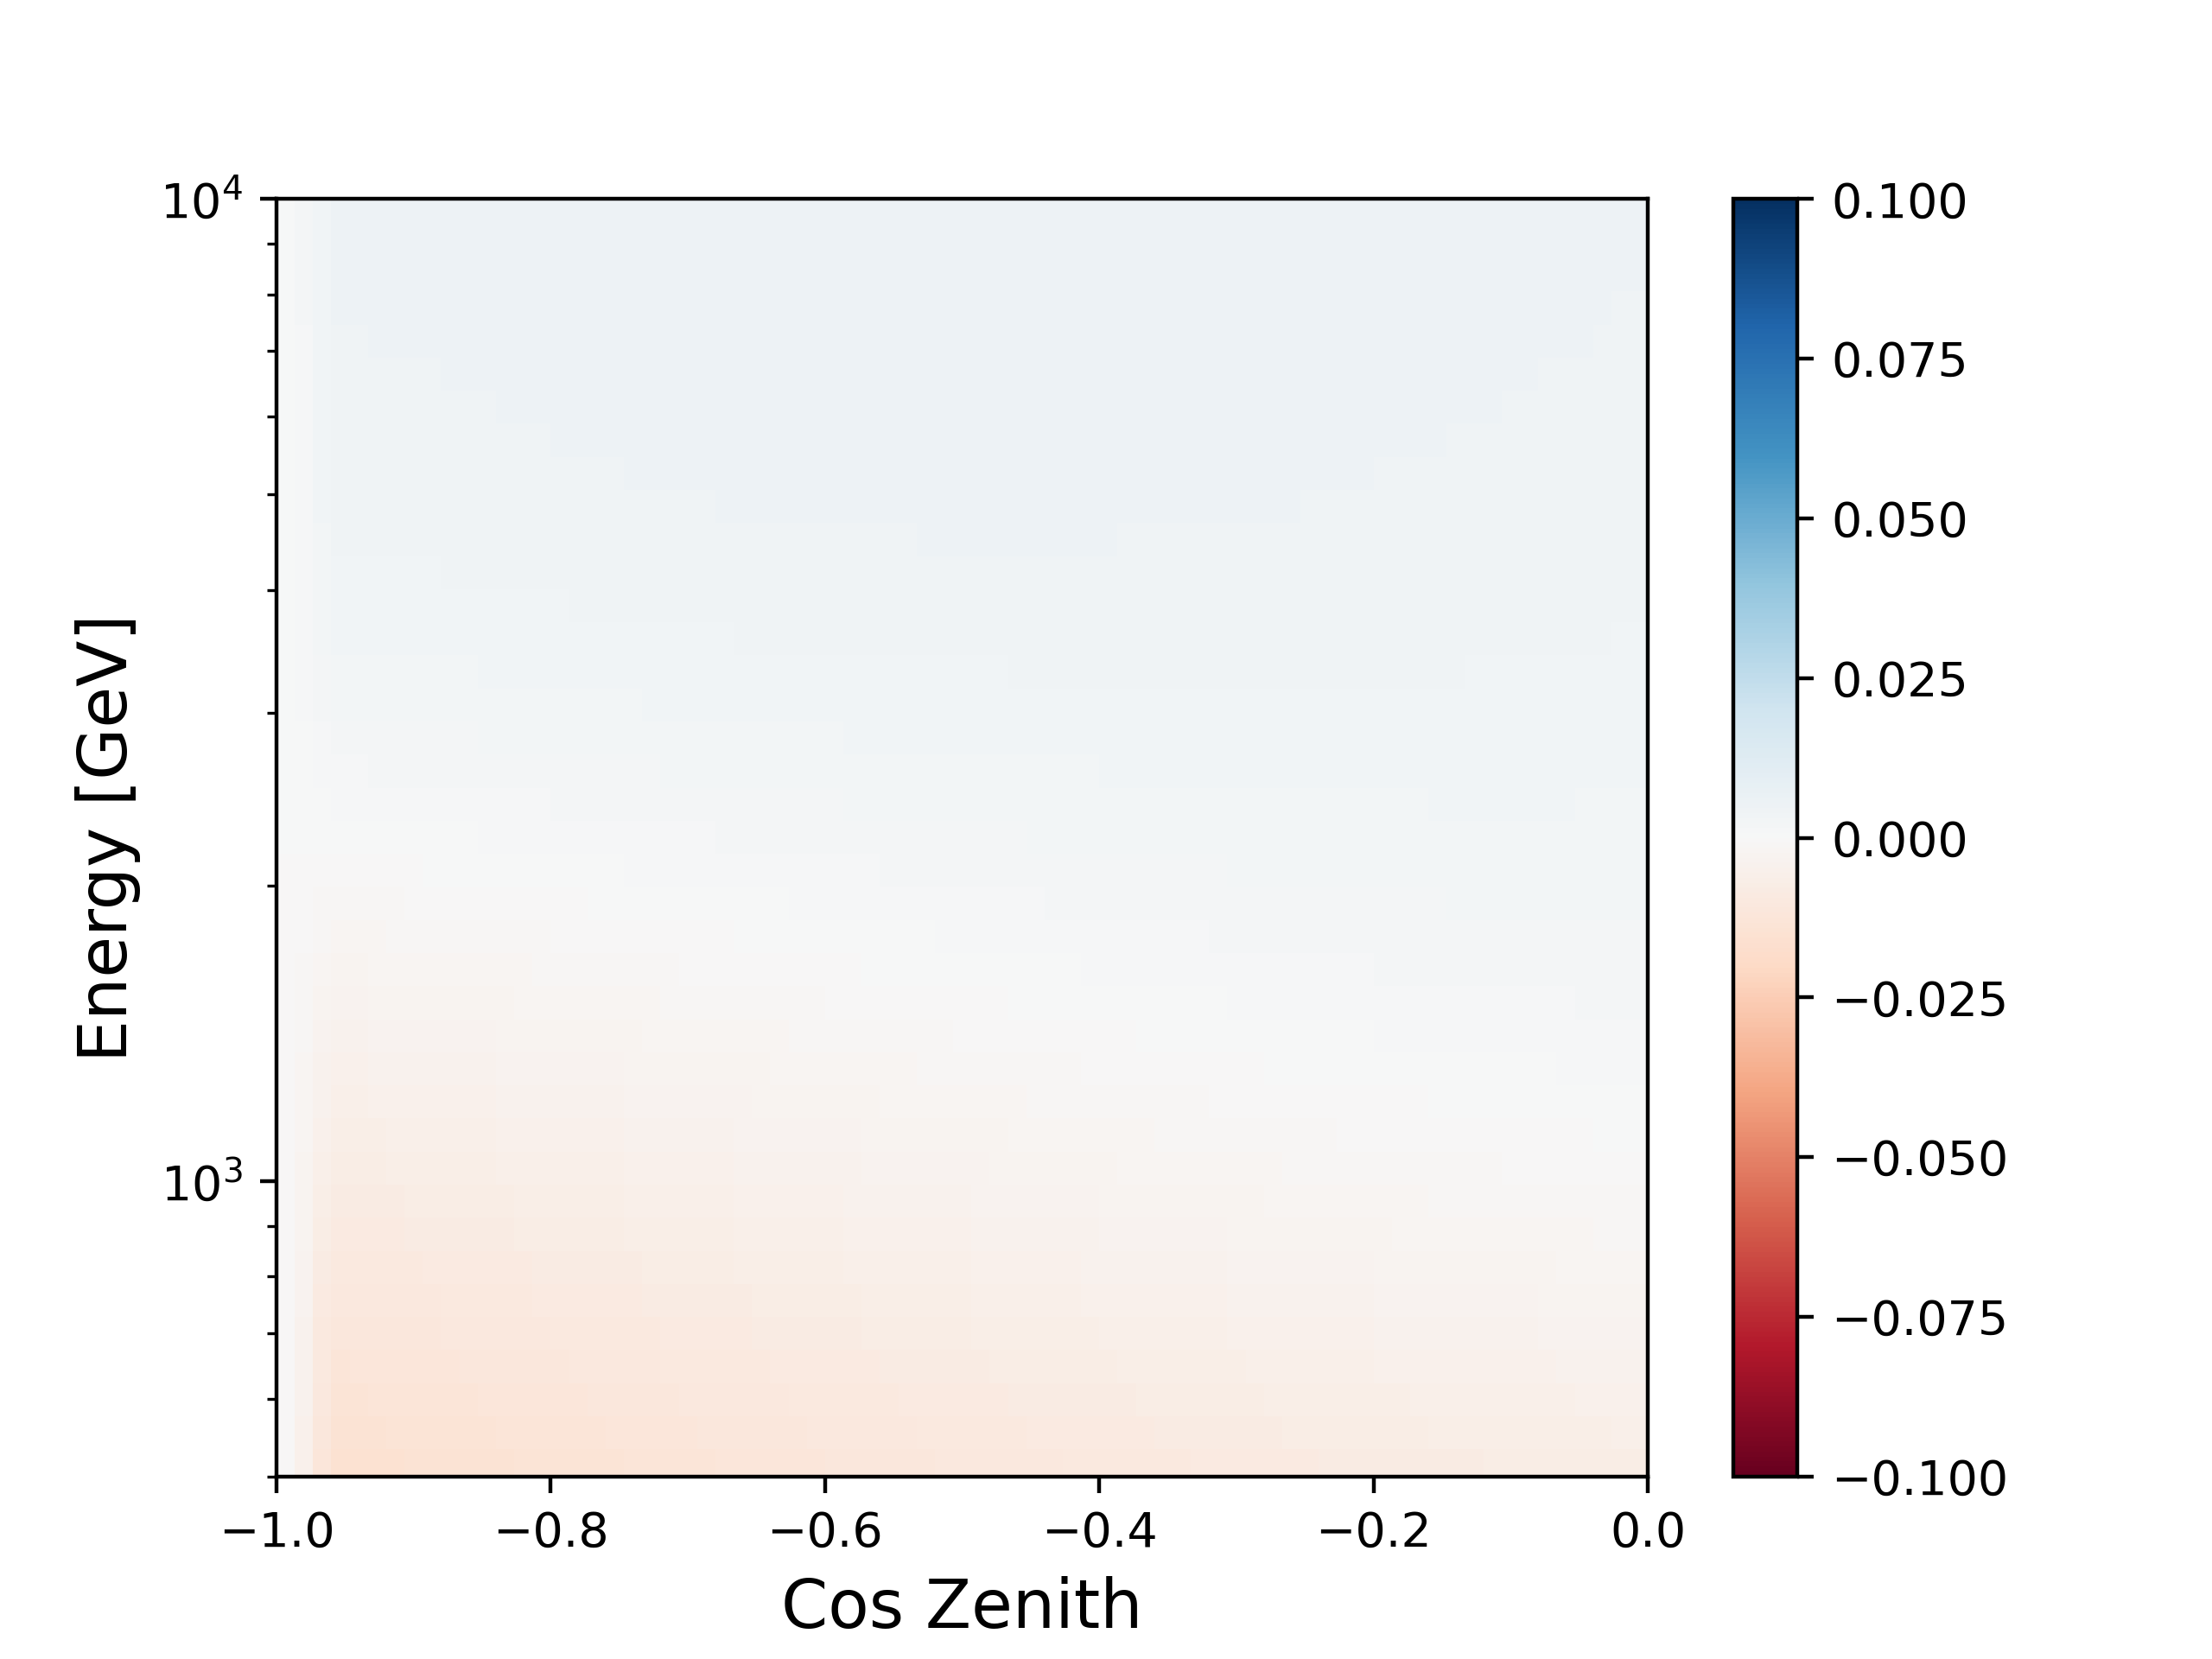
\includegraphics[width=0.3\linewidth]{figures/spline_phase02_gradient.png}%
    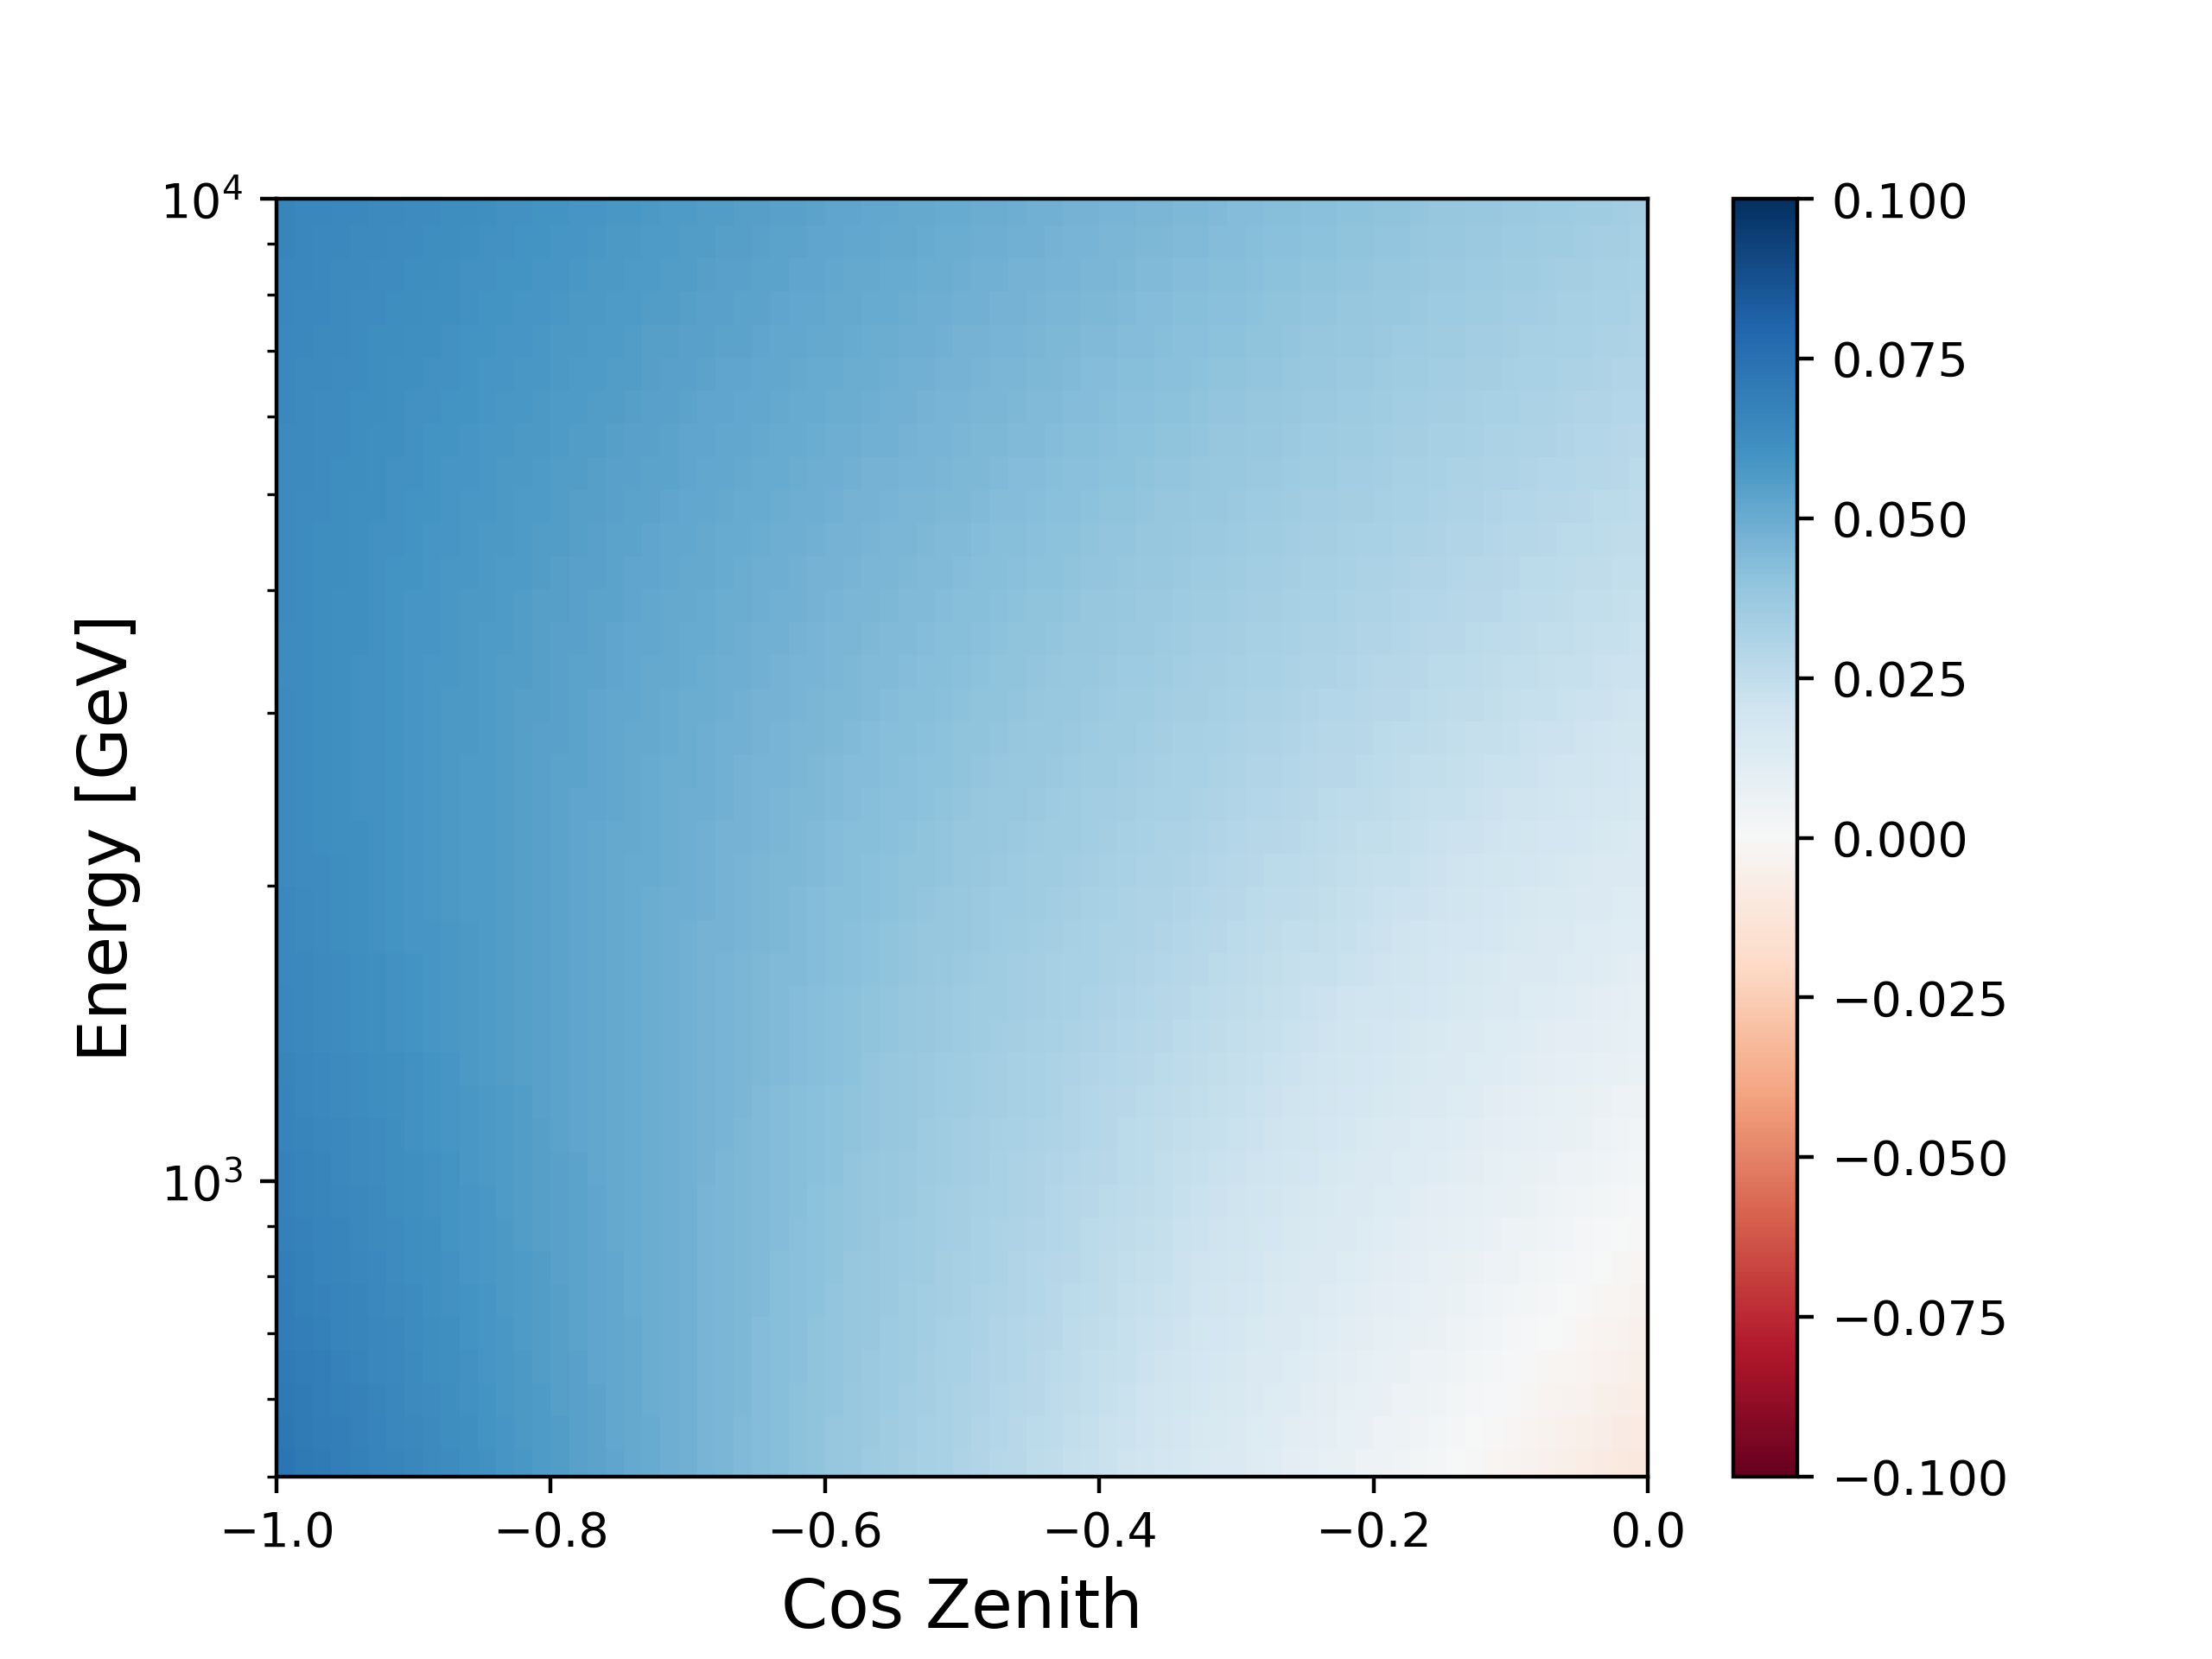
\includegraphics[width=0.3\linewidth]{figures/spline_phase03_gradient.png}%
    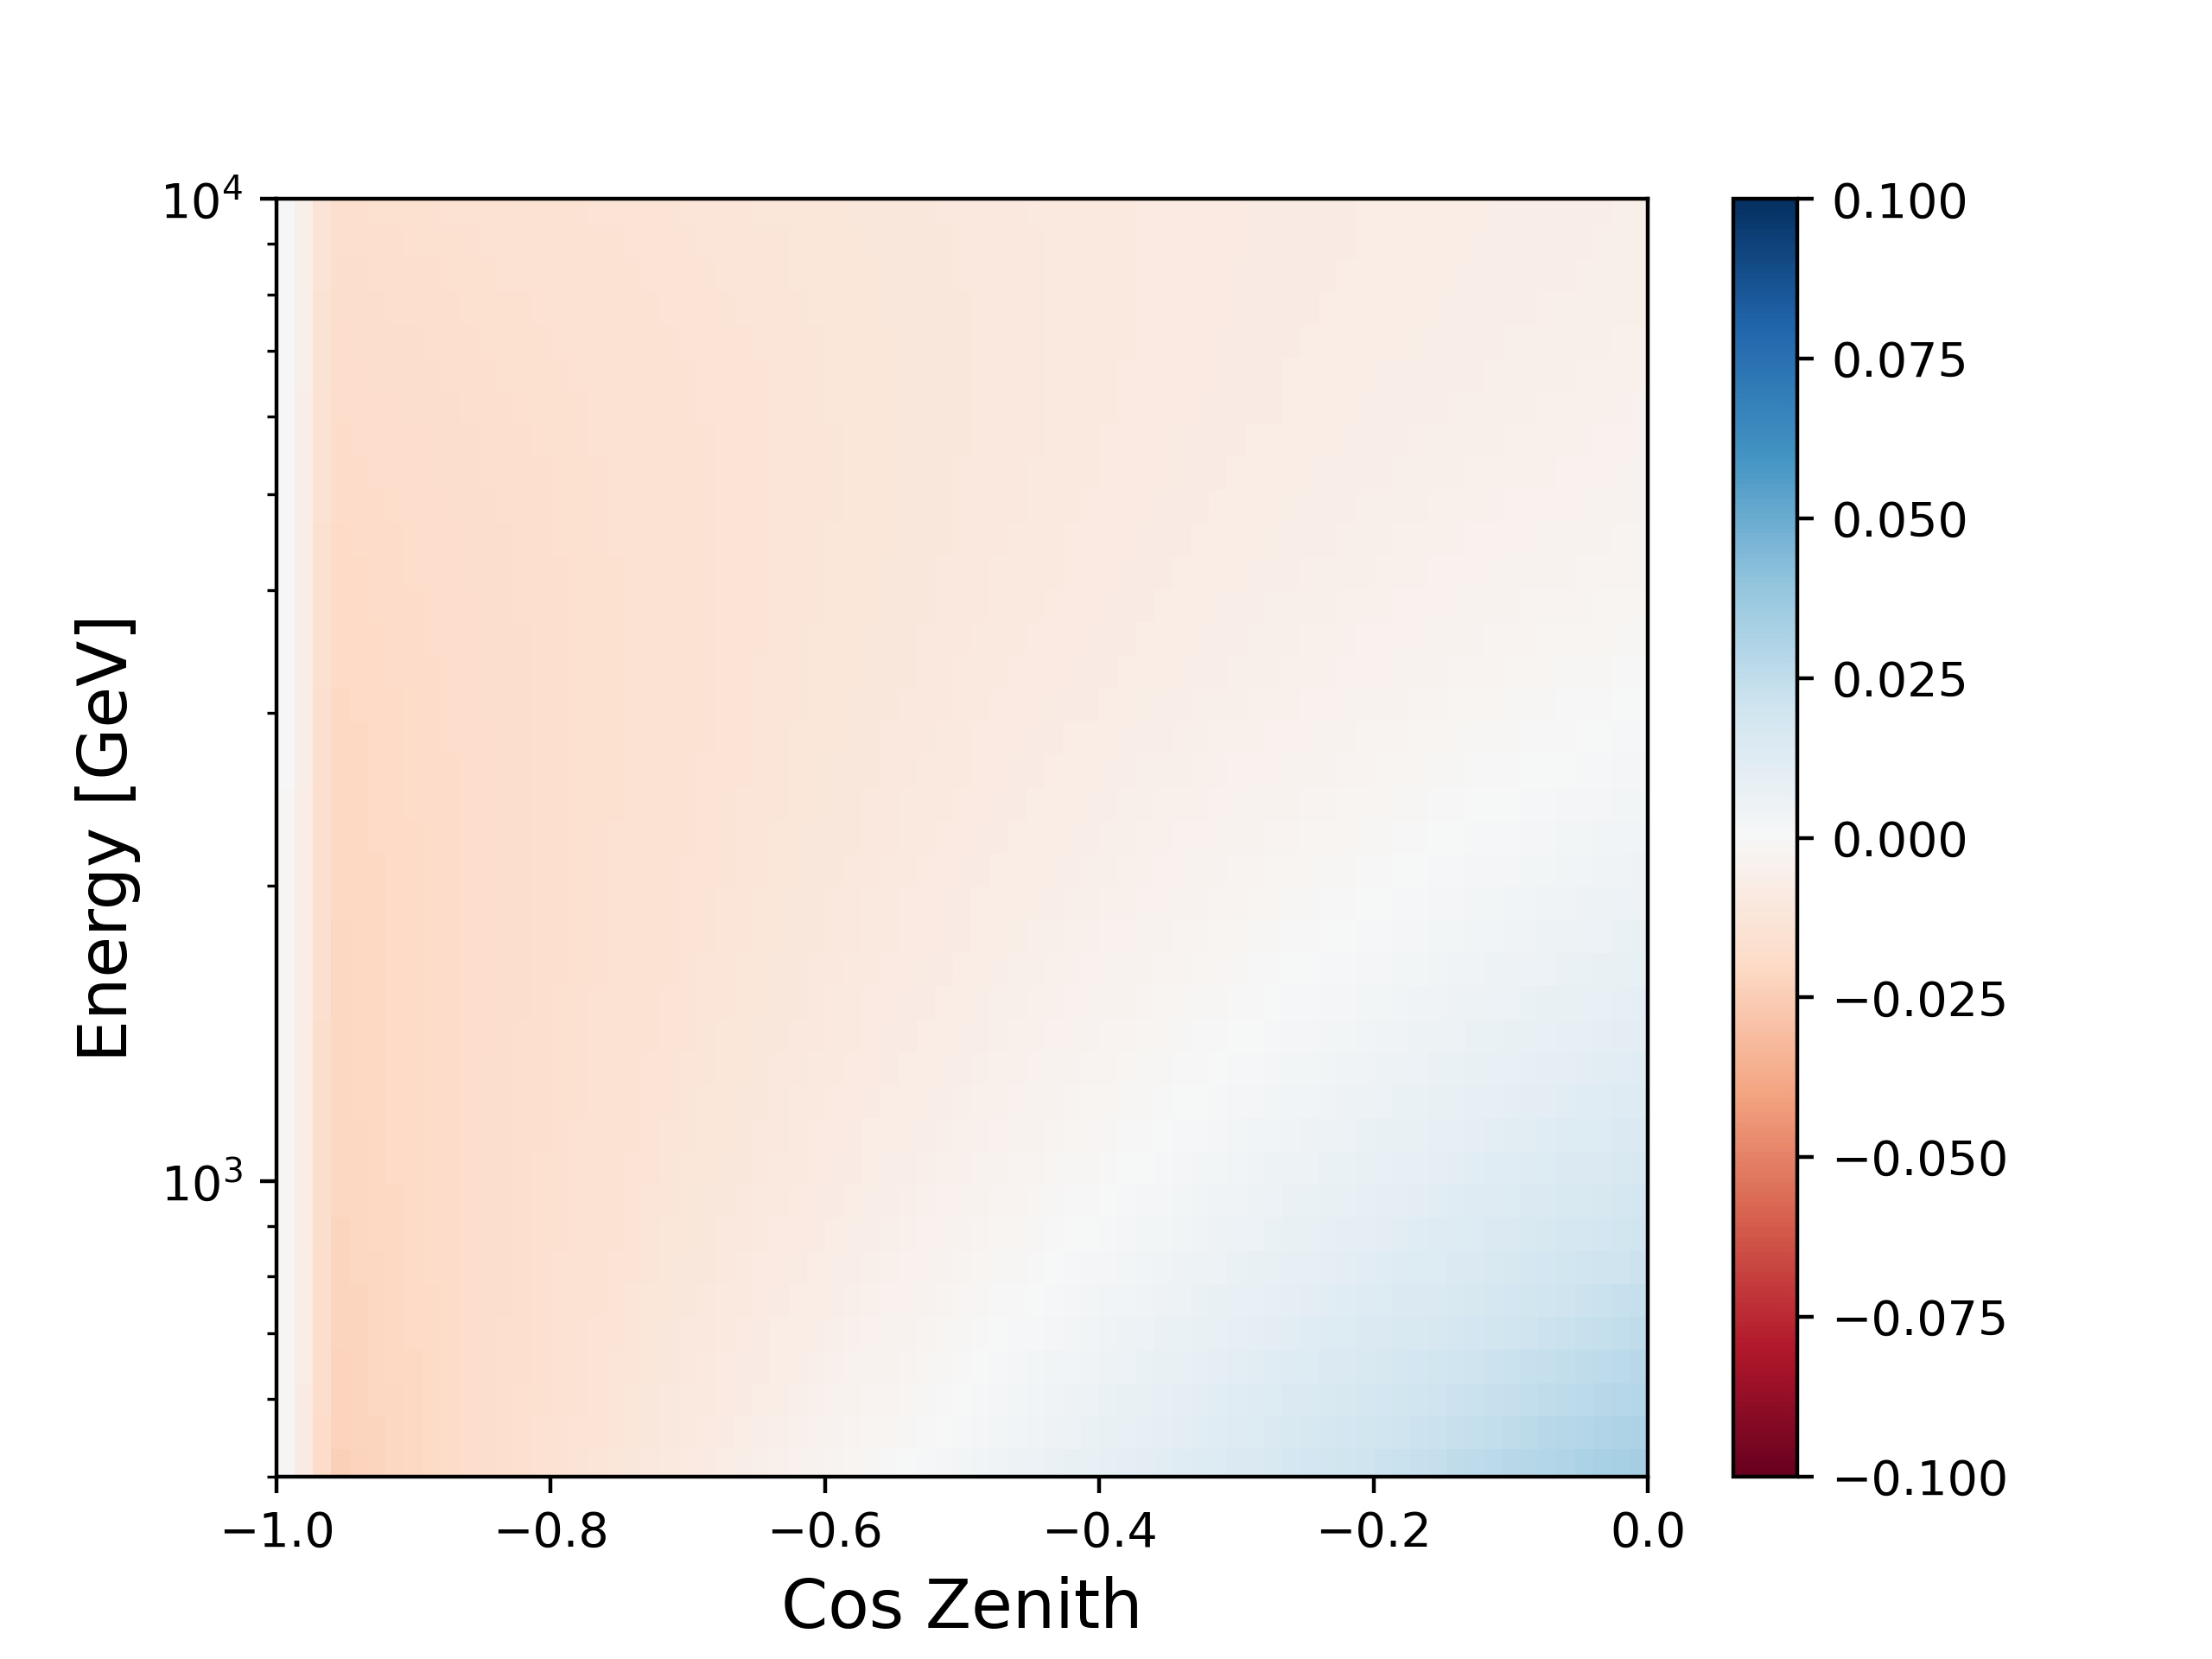
\includegraphics[width=0.3\linewidth]{figures/spline_phase04_gradient.png}
    \caption{Evaluations of the Photospline~\cite{WHITEHORN20132214} spline-fits to the 2D gradients as functions of energy and zenith. Left to right from top to bottom: Amplitude 0, Amplitude 1, Amplitude, 2, Amplitude 3, Amplitude 4, Phase 1, Phase 2, Phase 3, Phase 4.}\label{fig:gradients}
\end{figure}

Each of these were then implemented in our fitting framework, and the effects in analysis space were calculated. 
Using the previously calculated covariance matrix and the methods for de-correlating the nuisance parameters from Section~\ref{sect:down}, uncorrelated nuisance parameters were constructed as a simple basis change from the original amplitude/phase basis. 
Of the nine new parameters, only four were found to have a significant impact on analysis rates. The other five are kept at their central values in fits. 
The strongest four are shown in Figure~\ref{fig:rotata}.

\begin{figure}
    \centering
    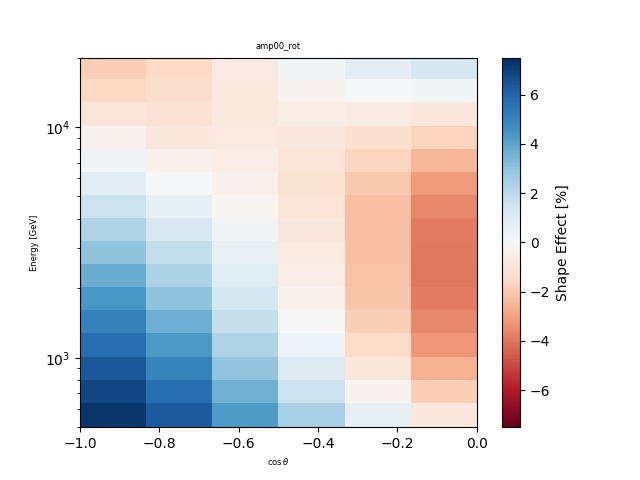
\includegraphics[width=0.45\linewidth]{figures/amp00_rot.png}%
    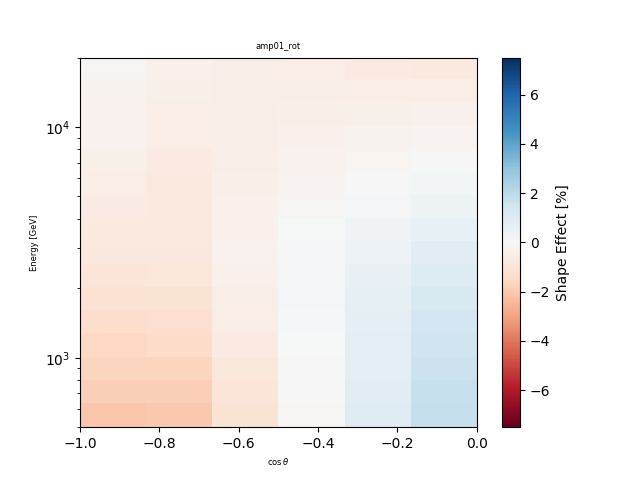
\includegraphics[width=0.45\linewidth]{figures/amp01_rot.png}\\
    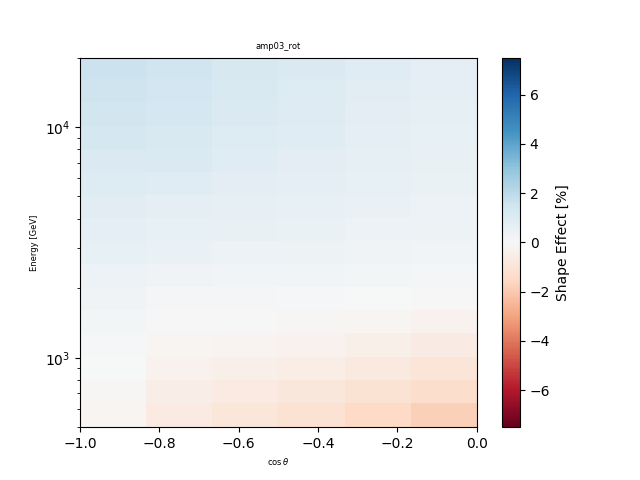
\includegraphics[width=0.45\linewidth]{figures/amp03_rot.png}%
    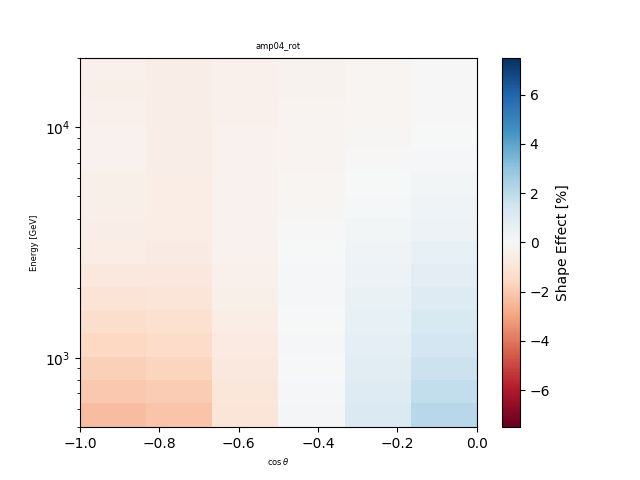
\includegraphics[width=0.45\linewidth]{figures/amp04_rot.png}
    \caption{Shape effects from perturbing each of the uncorrelated nuisance parameters by one sigma. Note that although named after phases and amplitudes, perturbing each of these is identical to perturbing a linear combination of all amplitudes and phases simultaneously.}\label{fig:rotata}
\end{figure}


\subsection{Hole Ice}

The hole ice represents a bubbly, refrozen region of ice around the DOMs. 
The bubbles, which formed during the refreezing, greatly decrease the scattering length of light. 
This has the effect of changing the light-acceptance of the DOMs as a function of photon incident angle. 
A plethora of different angular acceptance curves existed from various different calibration studies done to understand this region of the ice; and work was carried out to approximate these different curves and the space they spanned. 
Two separate hole ice models were used for the tracks and cascades; although it is expected that there are correlations between the priors, we expect that an uncorrelated fit to be a conservative approach in this context.  

\paragraph{Cascades}

For the cascades, spline-fits were carried out using seven support points and by forcing the acceptance to zero at the DOM backside (opposite the PMT). 
This resulted in six free, correlated, parameters needed to describe the acceptance curve. 
A principal component analysis was carried out, and it was found that all acceptance curves span a phase space of lower dimensionality. 
Only two components were needed to describe the space of angular acceptance curves, and those were named $p_{0}$ and $p_{1}$.
This is called the Unified Hole Ice Model.
The impacts of perturbing each one, individually, are demonstrated in Figure~\ref{fig:holeiceog}. 
In doing so, a small amount of error is introduced, though the overall uncertainty on the hole ice that remains is far greater than the introduced error. 

\begin{figure}
    \centering
    \begin{subfigure}{.45\textwidth}
        \centering
        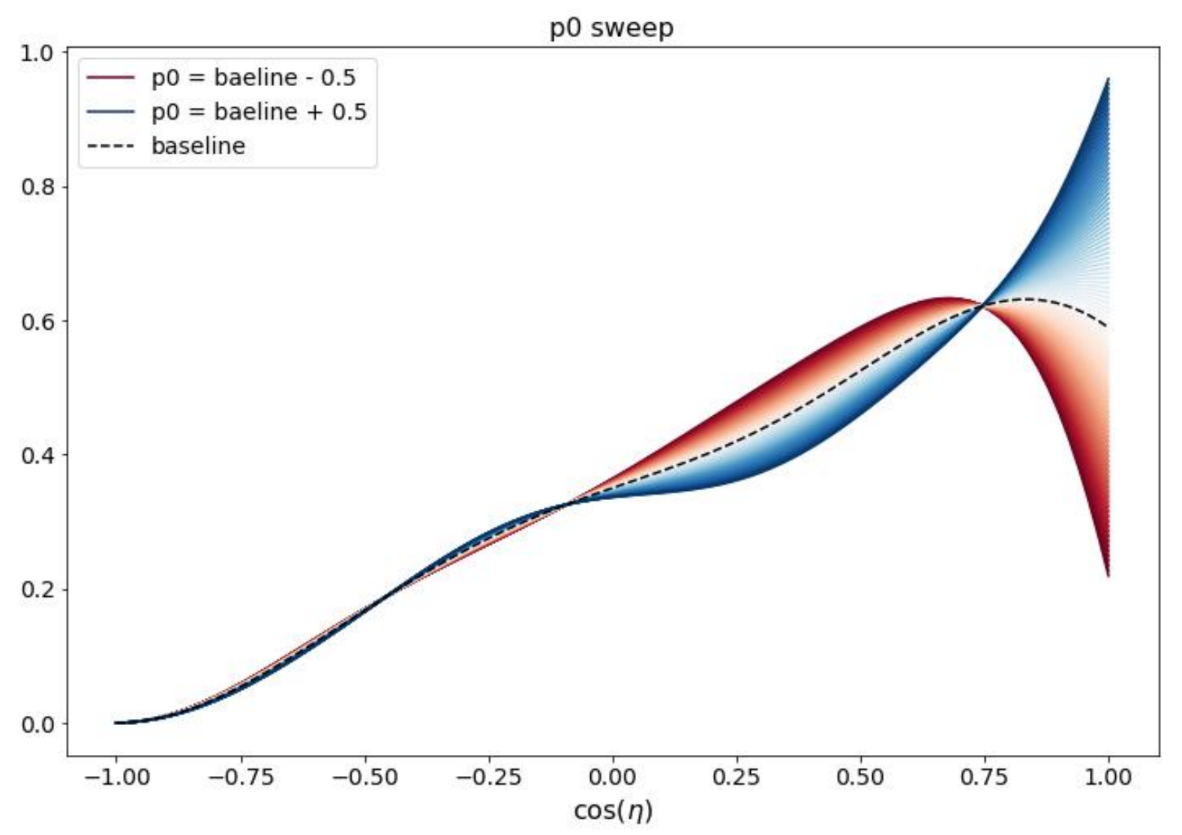
\includegraphics[width=0.95\linewidth]{./figures/holeice_p0_sweep.png}
        \caption{A sweep of the unified hole ice model $p_0$ parameter.}
    \end{subfigure}%
    \begin{subfigure}{.45\textwidth}
        \centering
        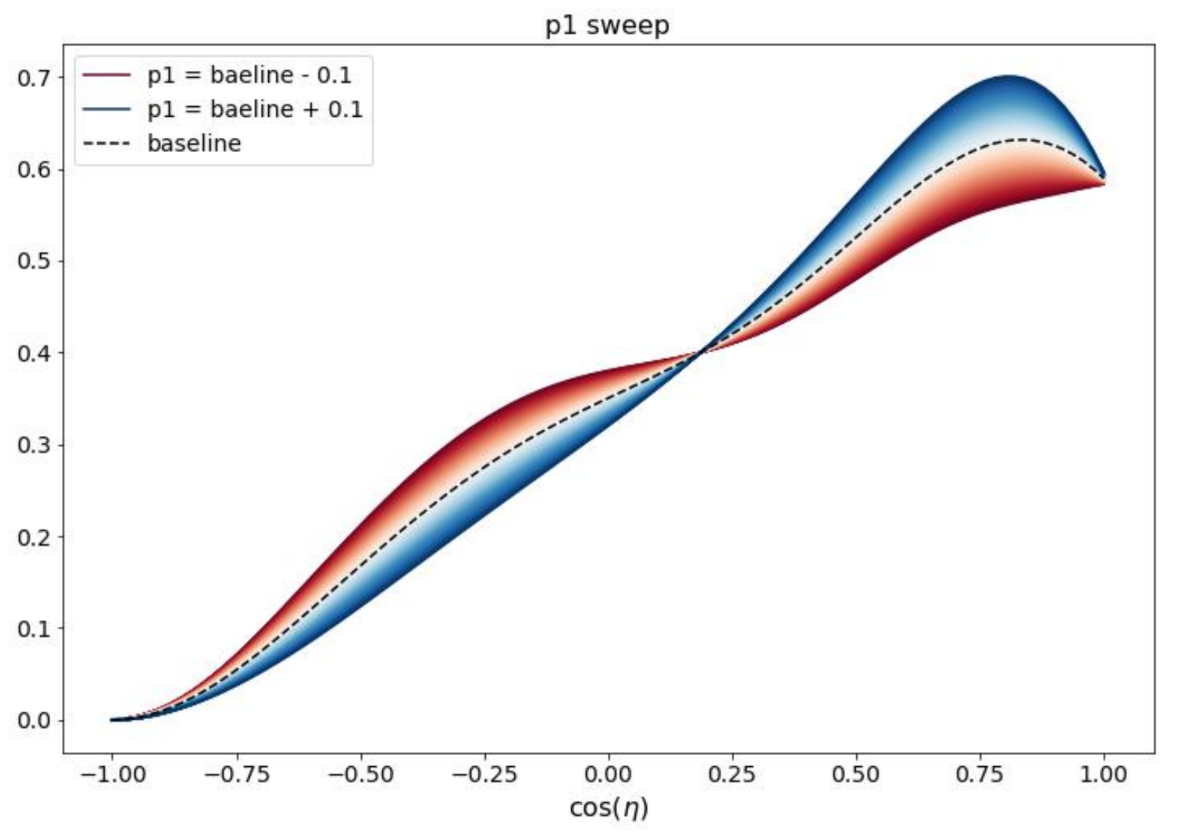
\includegraphics[width=0.95\linewidth]{./figures/holeice_p1_sweep.png}
        \caption{A sweep of the unified hole ice model $p_1$ parameter.}
    \end{subfigure}
    \caption{Effects of varying unified hole ice model parameters. $\eta$ represents angle of photon incidence on the DOM; -1 is the DOM backside, and +1 is the DOM PMT face.}\label{fig:holeiceog}
\end{figure}

\begin{figure}
    \centering
    \begin{subfigure}{.48\textwidth}
        \centering
        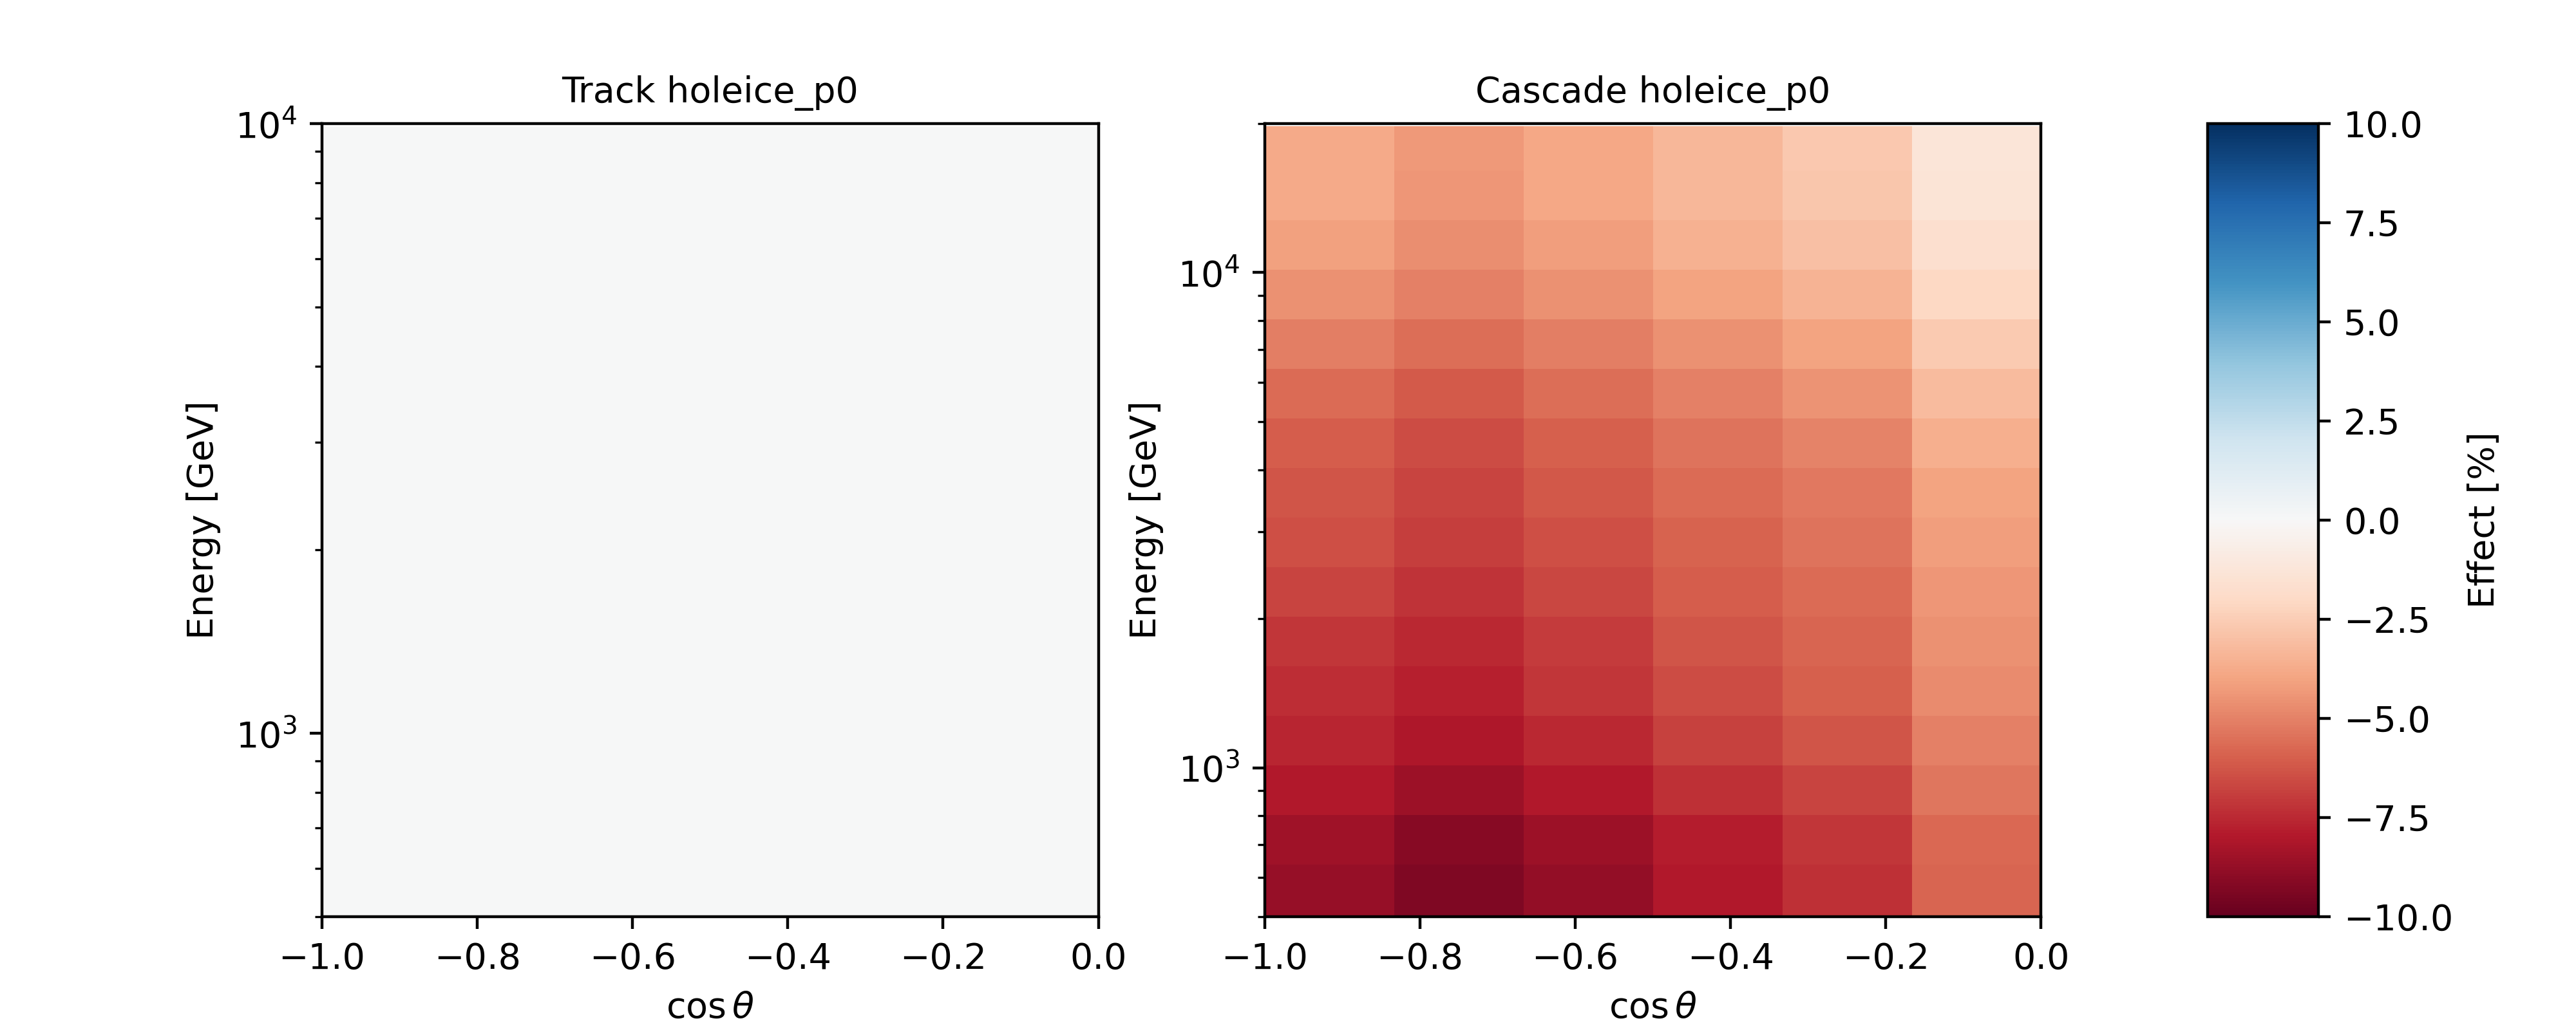
\includegraphics[width=0.95\linewidth]{./figures/systematics/holeice_p0.png}
        \caption{A sweep of the unified hole ice model $p_0$ parameter.}
    \end{subfigure}%
    \begin{subfigure}{.48\textwidth}
        \centering
        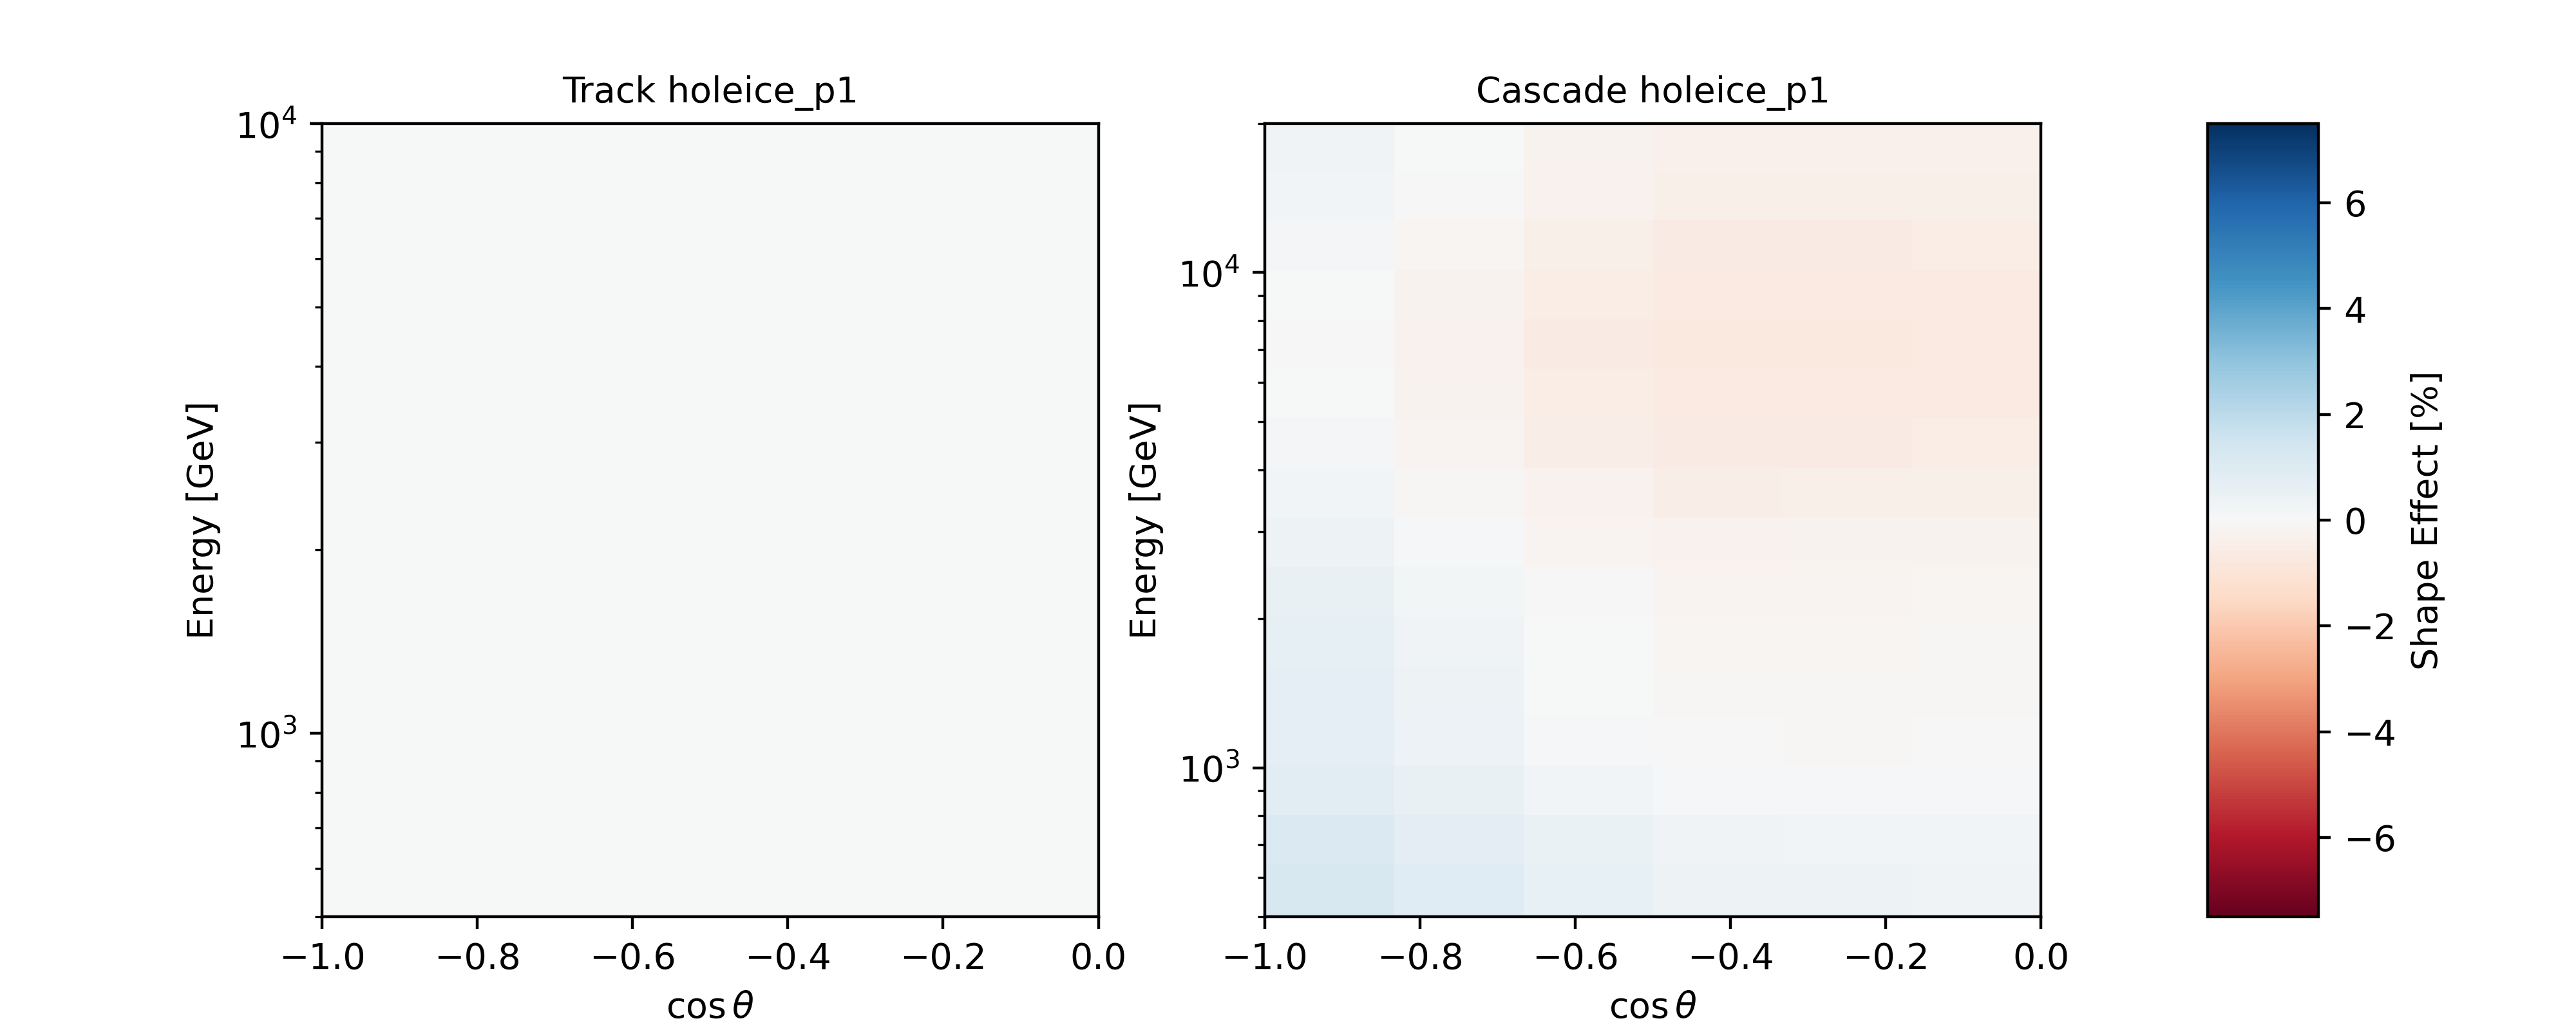
\includegraphics[width=0.95\linewidth]{./figures/systematics/holeice_p1.png}
        \caption{A sweep of the unified hole ice model $p_1$ parameter.}
    \end{subfigure}
    \caption{Effects of varying unified hole ice model parameters. $\eta$ represents angle of photon incidence on the DOM; -1 is the DOM backside, and +1 is the DOM PMT face.}\label{fig:holeiceparmas}
\end{figure}

Like the DOM Efficiency, a SnowStorm MC ensemble was prepared for the cascades sample in which the hole ice parameters $p_{0}$ and $p_{1}$ were allowed to vary. 
For each batch of ten simulated MC events these parameters $p_{0}$ and $p_{1}$ are randomly sampled uniformly from the ranges $p_{0}\in\left[-0.84, 0.3\right]$ and $p_{1}\in\left[-0.134, 0.05\right]$. 
The angular acceptance of the DOMs in CLSim is then manually adjusted according to the new angular acceptance and the photon propagation is then carried out. 
The remainder of the MC simulation chain is then performed as usual.

The SnowStorm technique is applied to this MC sample using the cutting technique described in Ref~\cite{Aartsen_2019_snow}, and the 2D analysis gradients are constructed. 
These are shown in Figure~\ref{fig:holeiceparmas}. 

\paragraph{Tracks}

The track sample uses a previous implementation originally developed for Ref~\cite{Aartsen_2020_prd}.
Several MC samples were generated according to an angular acceptance model parametrized by 
\begin{equation}
    \mathcal{A}(\eta) = 0.34\left(1+ 1.5\cos\eta - \cos^{3}\eta/2\right) + p_{1}\cos\eta\left(\cos^{2}\eta - 1\right)^{3} + p_{2}\exp\left(10(\cos\eta - 1.0)\right)
\end{equation}
where $\mathcal{A}$ is the relative acceptance of the DOMs as a function of $eta$, the angle of photon incidence on the DOM. 
This is plotted for various values of $p_{1}$ and $p_{2}$ in Figure~\ref{fig:forwardholceice}.

\begin{figure}
    \centering
    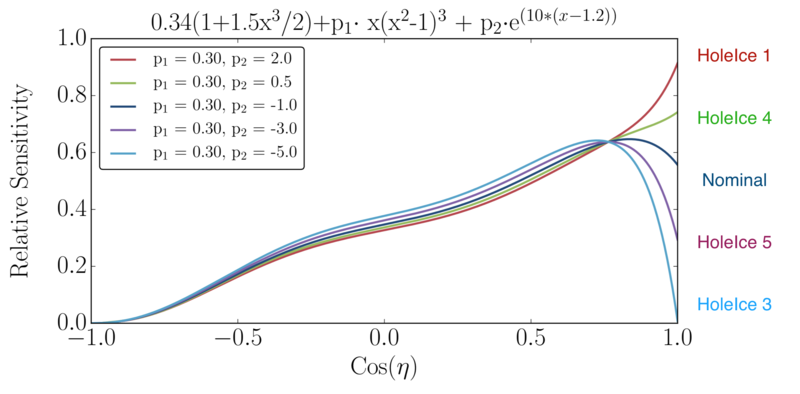
\includegraphics[width=0.8\linewidth]{figures/forward_holeice.png}
    \caption{The hole ice parametrization of the MSU hole ice model. The H2 model is an earlier model used and developed internally.}\label{fig:forwardholceice}
\end{figure}

A nominal sample was generated using $p_{1}=0.3$ and $p_{2}=-1.0$, and then support points were generated at $p_{2}$ values of -5, -3, -1, 0.5, and 2.
A 3D spline-fit was carried out over $p_{2}$, $\log E$, and $\cos\theta$; the $p_{1}$ parameter was observed to have a negligible effect on reconstructed rates. 
The effects of perturbing this parameter on the reconstructed rates are shown in Figure~\ref{fig:track_hole}.

\begin{figure}
    \centering
    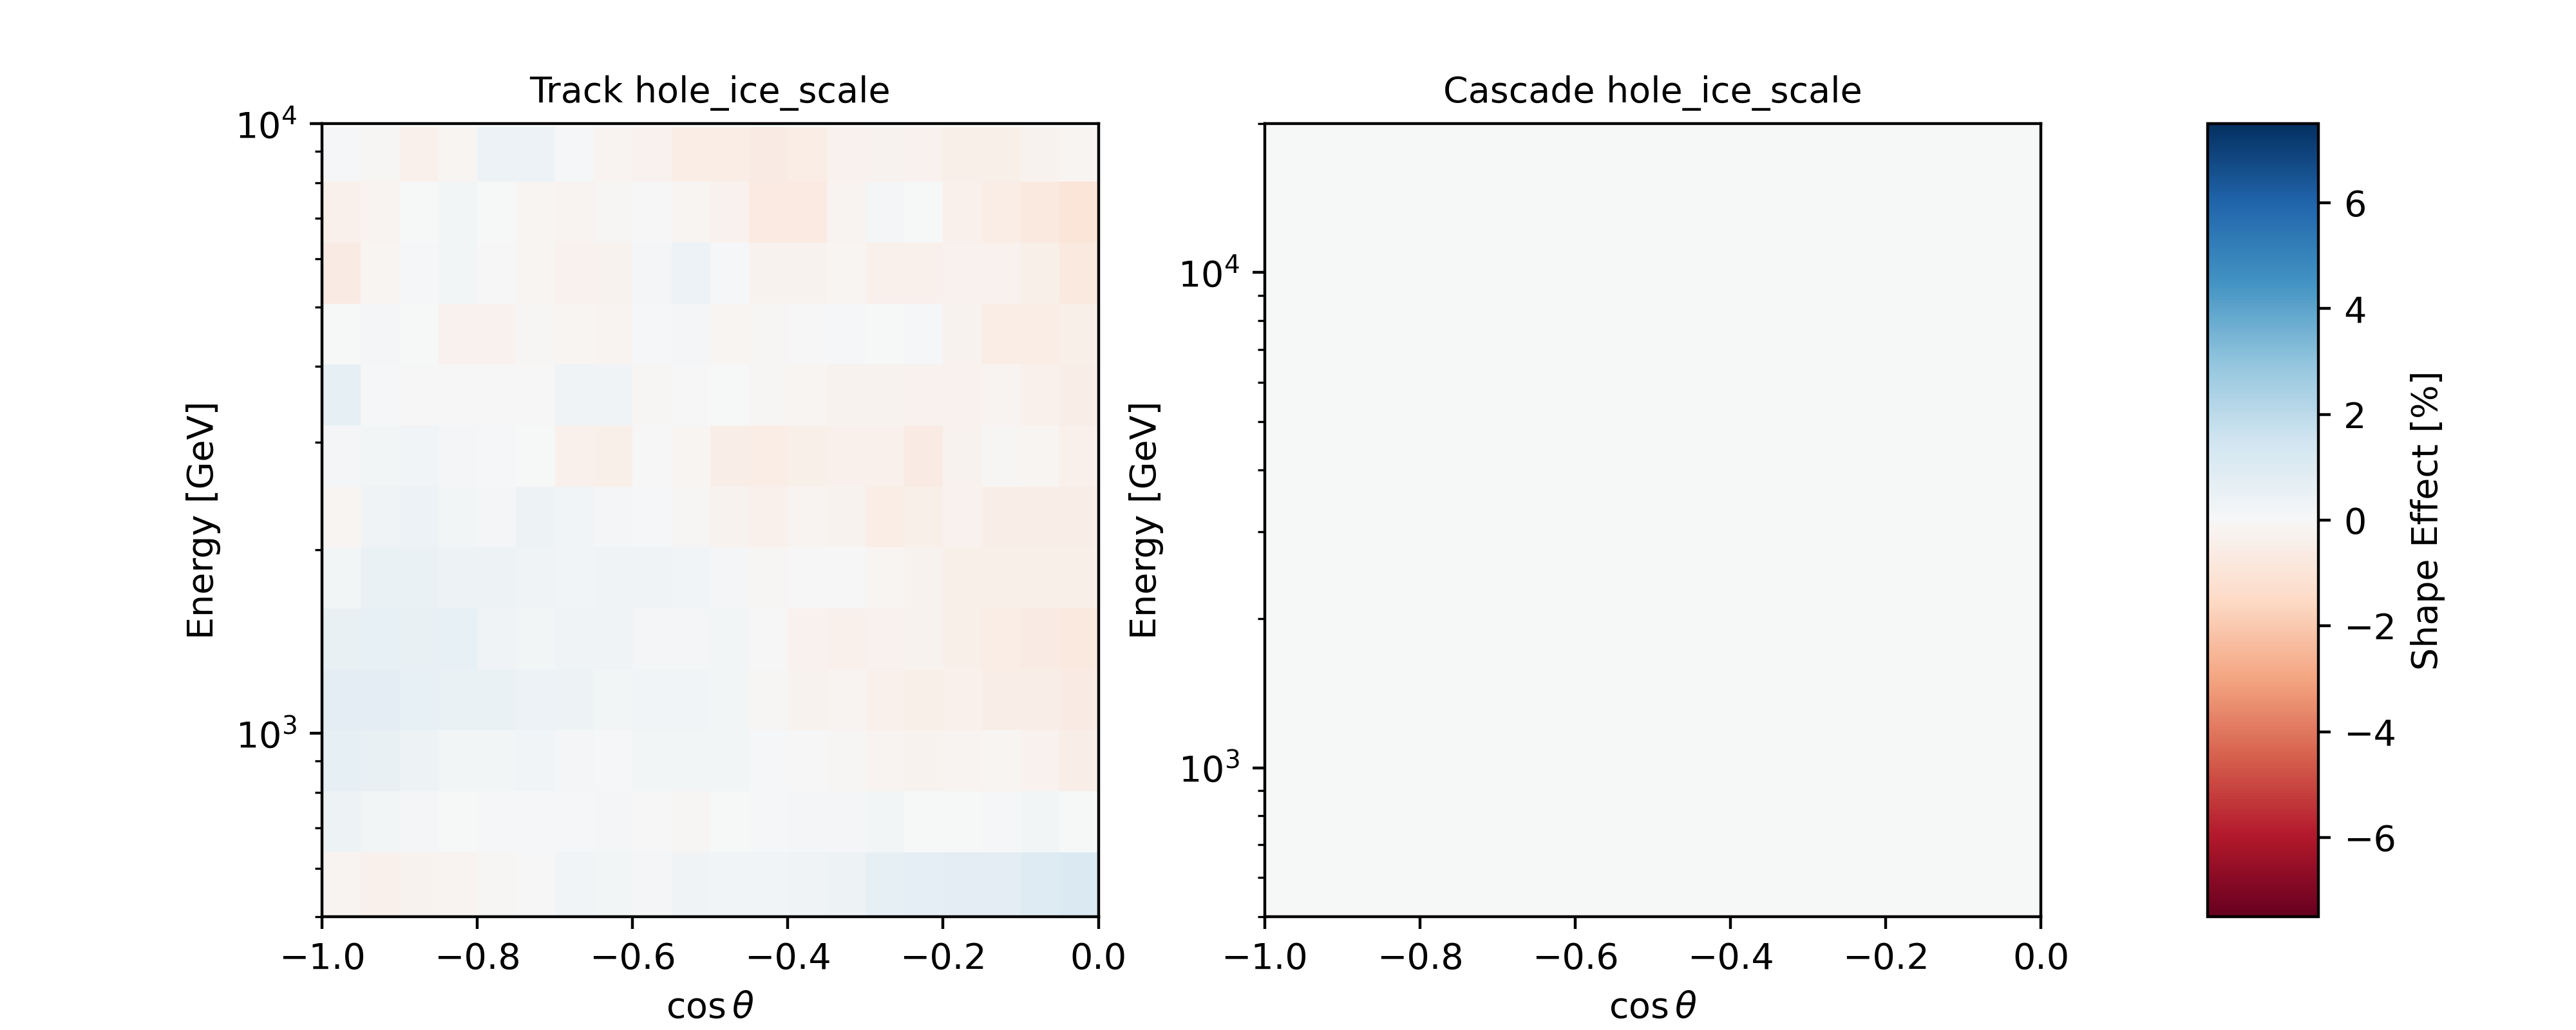
\includegraphics[width=0.8\linewidth]{figures/systematics/hole_ice_scale.png}
    \caption{The effects of perturbing the track sample's hole ice parameter on the track sample (left) and cascades sample (right).}\label{fig:track_hole}
\end{figure}

\subsection{Atmospheric Neutrino Flux}
\index{neutrino!flux}
Previous studies, in particular the 8-year track-only analysis~\cite{Aartsen_2020,Aartsen_2020_prd}, have used an uncertainty on the normalization and spectral index for the cosmic ray flux, and modeled uncertainties on the production of pions and kaons in the air showers using the Barr parametrization~\cite{PhysRevD.74.094009}. 
In this analysis, we now use the DAta-rivEn MuOn-calibrated Neutrino Flux~\cite{yanez2023daemonflux} (DaemonFlux) model, which incorporates uncertainties estimated for both fixed-target and cosmic ray experimental results, as both our baseline flux prediction and as a method of parametrizing uncertainties in our flux prediction. 
This model implements parameters effecting particle production rates of protons, neutrons, $\pi^{\pm}$, and $K^{\pm}$ at four different energy scales, along with six parameters from a principal component analysis of a global spline fit of the cosmic ray flux. 
From the fits to the data, a correlated prior is determined for the full ensemble of 24 parameters, as shown in Figure~\ref{fig:daemon_cor}.
\begin{figure}
    \centering
    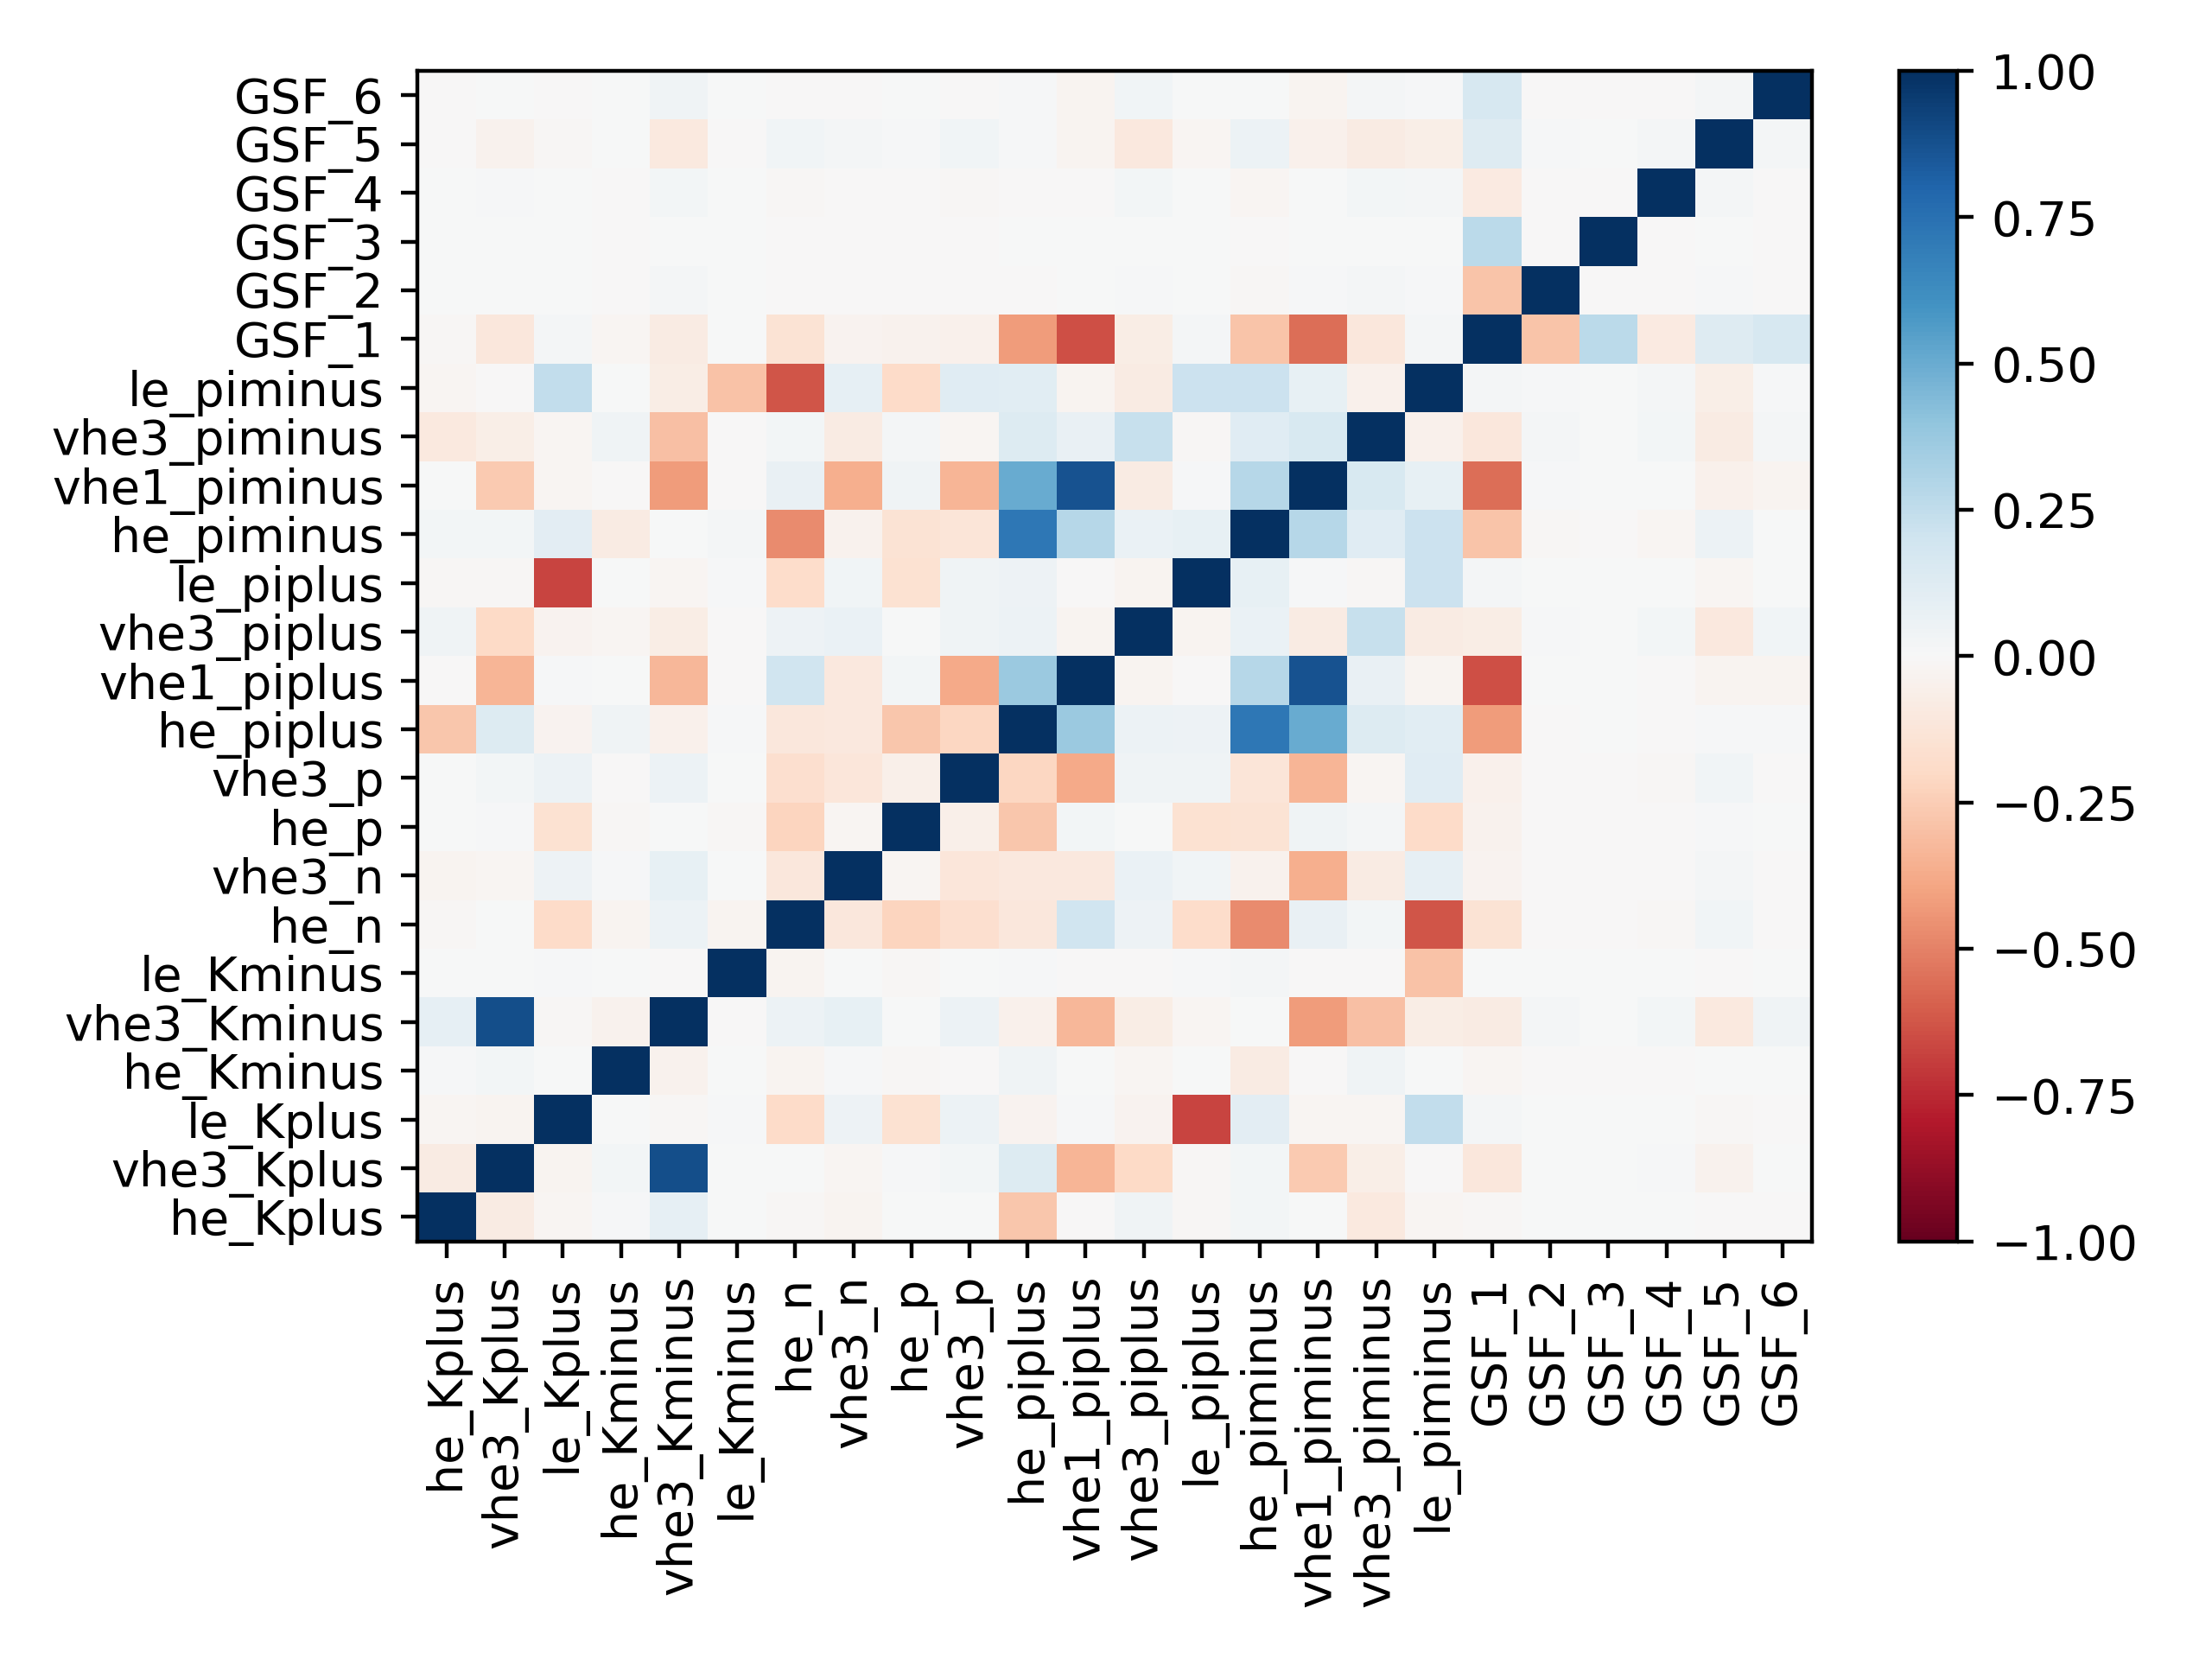
\includegraphics[width=0.7\linewidth]{figures/daemon_cov.png}
    \caption{The correlation between the parameters used in the DaemonFlux model.}\label{fig:daemon_cor}
\end{figure}

For this analysis, the effects of perturbing each of these 24 parameters are evaluated after a one-sigma from their central values.
From these perturbed fluxes and the central expectations, we extract the flux-gradients for each of these parameters.
These neutrino flux gradients are then evolved using nuSQuIDS to get the full-flavor gradient flux at IceCube. 
The effects of perturbing each parameter, independently, is shown for the cascades sample assuming no sterile neutrino in Figure~\ref{fig:daemon_grads}.
It is observed that only a small subset of all 24 parameters were relevant for this analysis. 
The procedures described in Section~\ref{sect:down} were first carried out to identify the strongest parameters in the uncorrelated basis. 
Random expectations were then sampled from the full DaemonFlux ensemble, and fits were carried out while allowing the $n$, strongest, uncorrelated parameters to float. 
The distributions of the resulting $\Delta LLH$ values of these fits were logged after running over a thousand fits for both cascades and tracks, separately, and are shown in Figure~\ref{fig:daemon_number} for tracks (left) and cascades (right). 

It was also observed that the same parameters had the strongest effects on both the track and cascade expectations, and that only 7 parameters are necessary to sufficiently span the expectation-space; eight were used to be conservative. 
As an additional check, fits were carried out using two different numbers of free parameters while injecting different sterile neutrino signals. 
These results are shown in Table~\ref{tab:daemonfluxfit}

The effects of pertubing the eight strongest parameters by one sigma are shown for both tracks and cascades in Figures~\ref{fig:daemon_analysis_one} and~\ref{fig:daemon_analysis_two}.

\begin{figure}
    \centering
    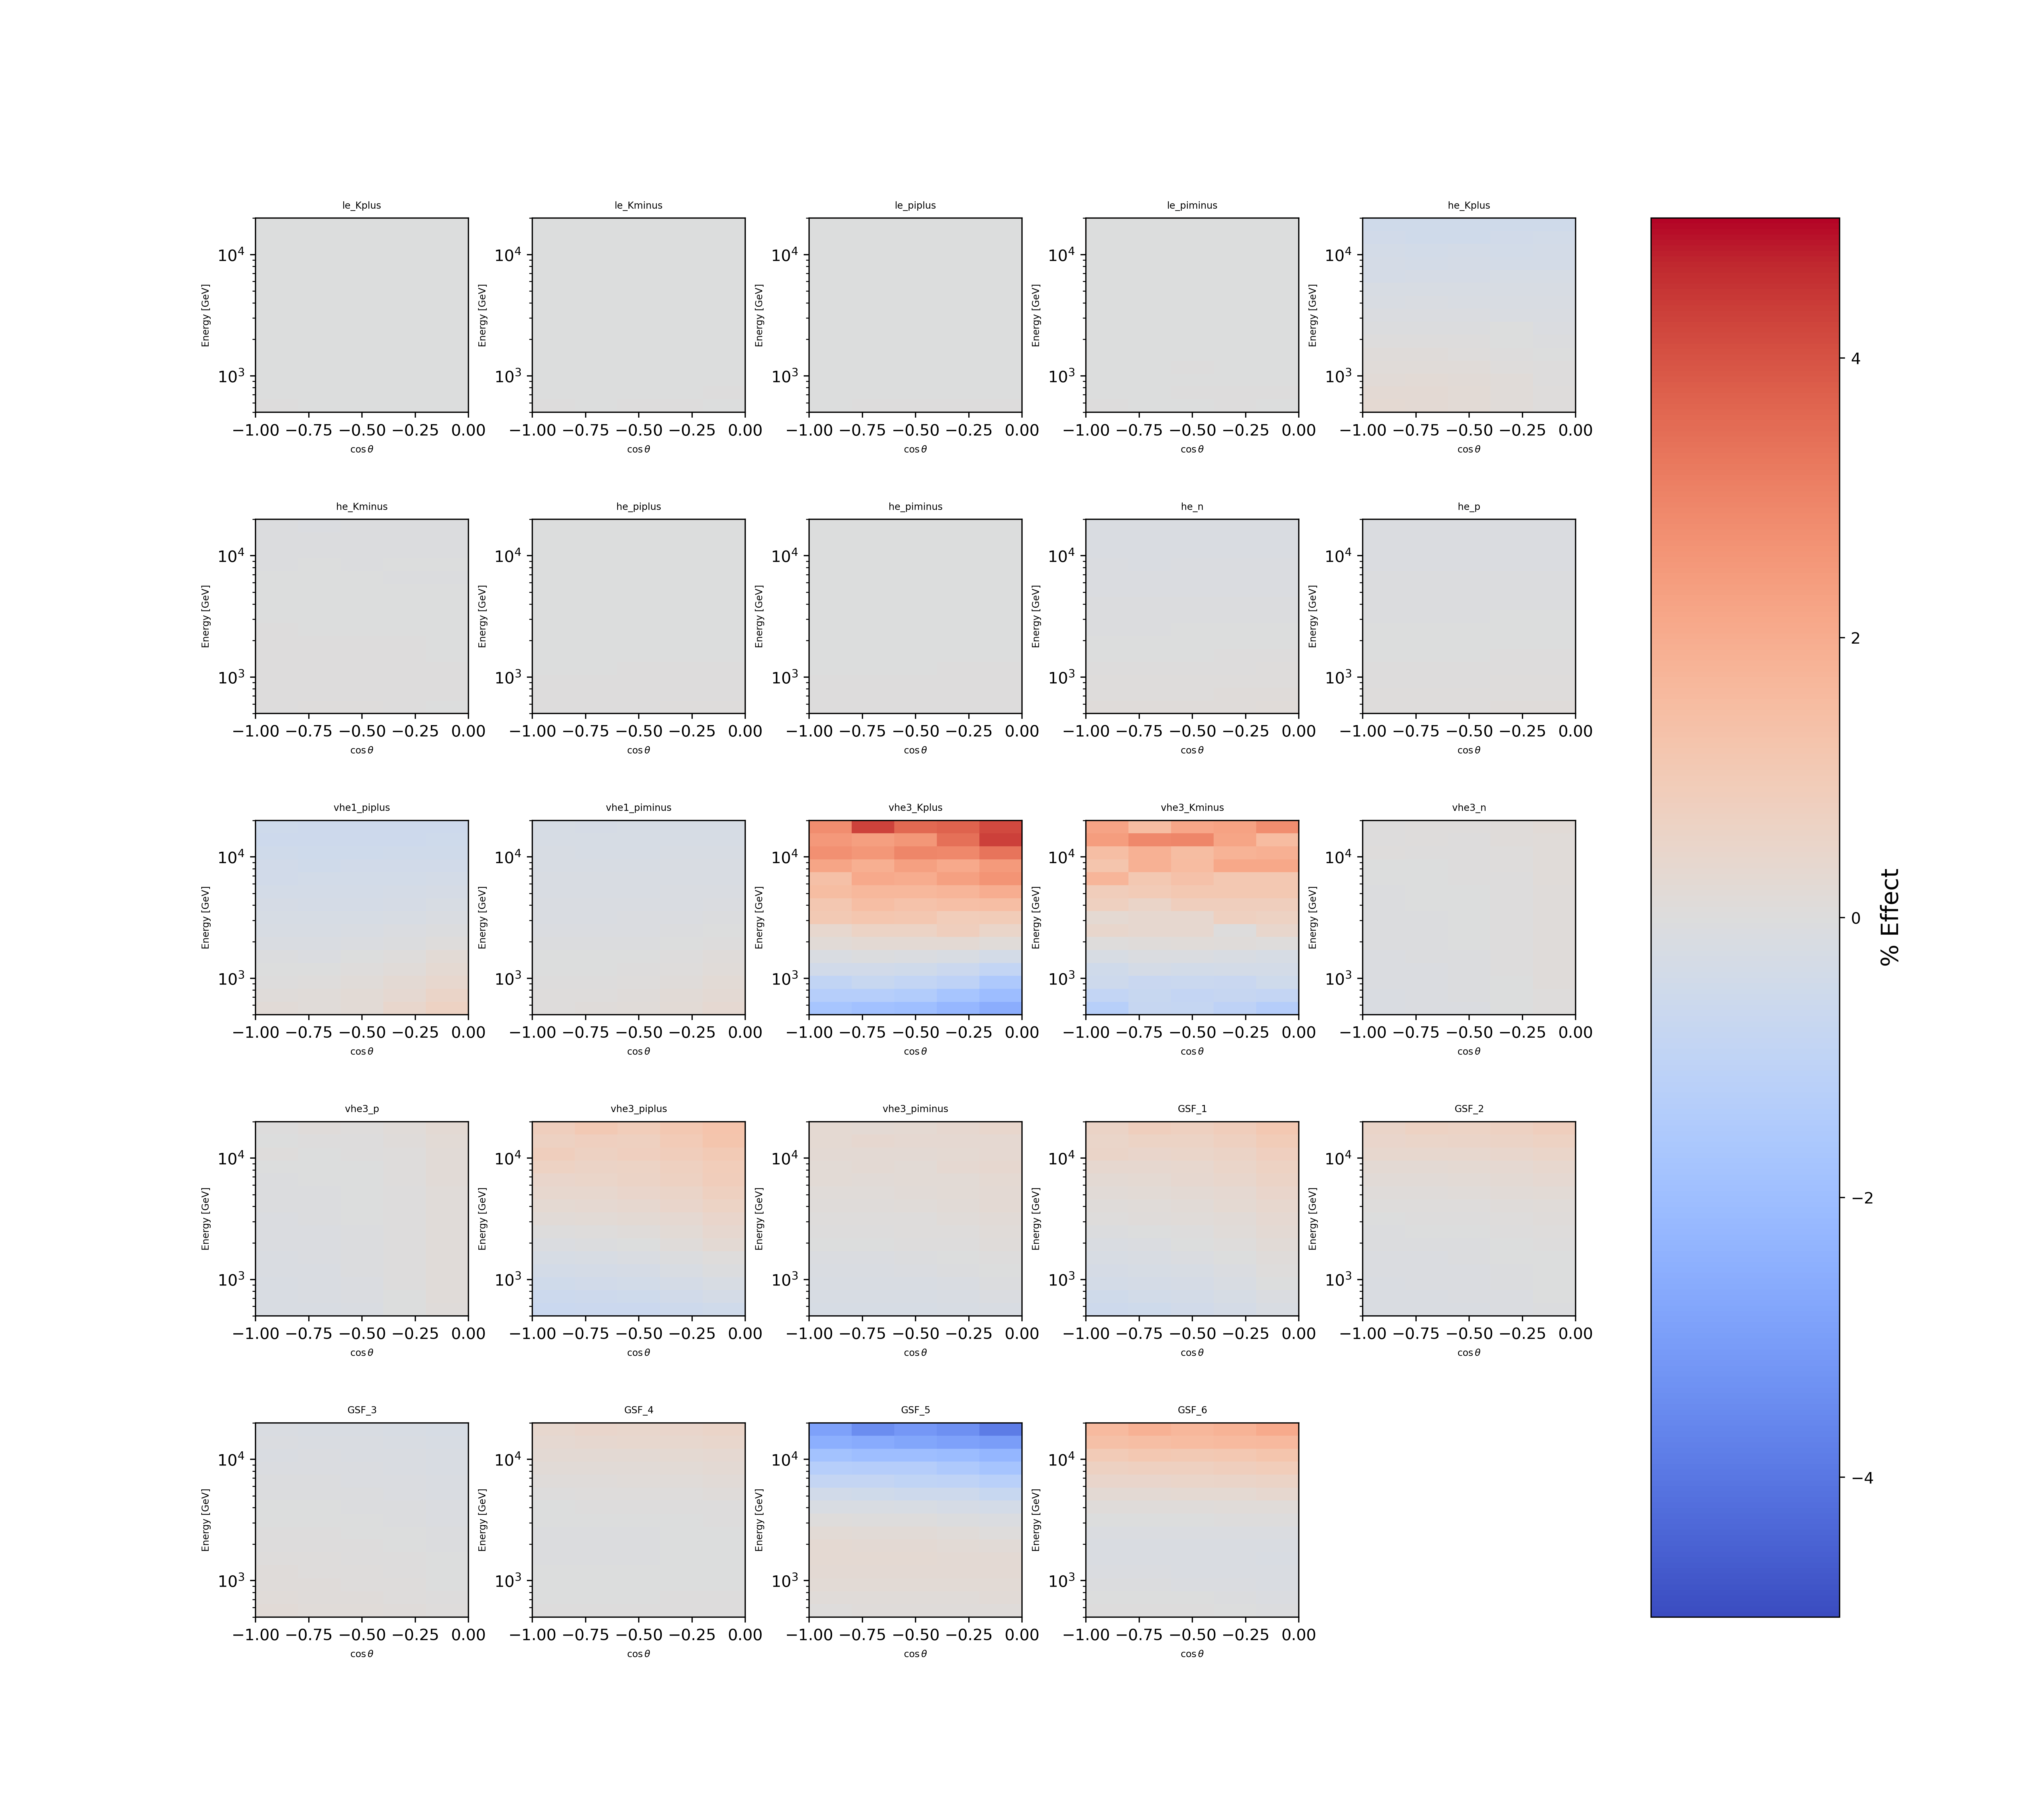
\includegraphics[width=0.9\linewidth]{figures/all_grads.png}
    \caption{Shape-effect of perturbing each of the 24 DaemonFlux nuisance parameters by one-sigma in analysis space. Plots here are showing the effects on the cascades sample; the effects on the track sample have been observed to be extremely similar.}\label{fig:daemon_grads}
\end{figure}

\begin{figure}
    \centering 
    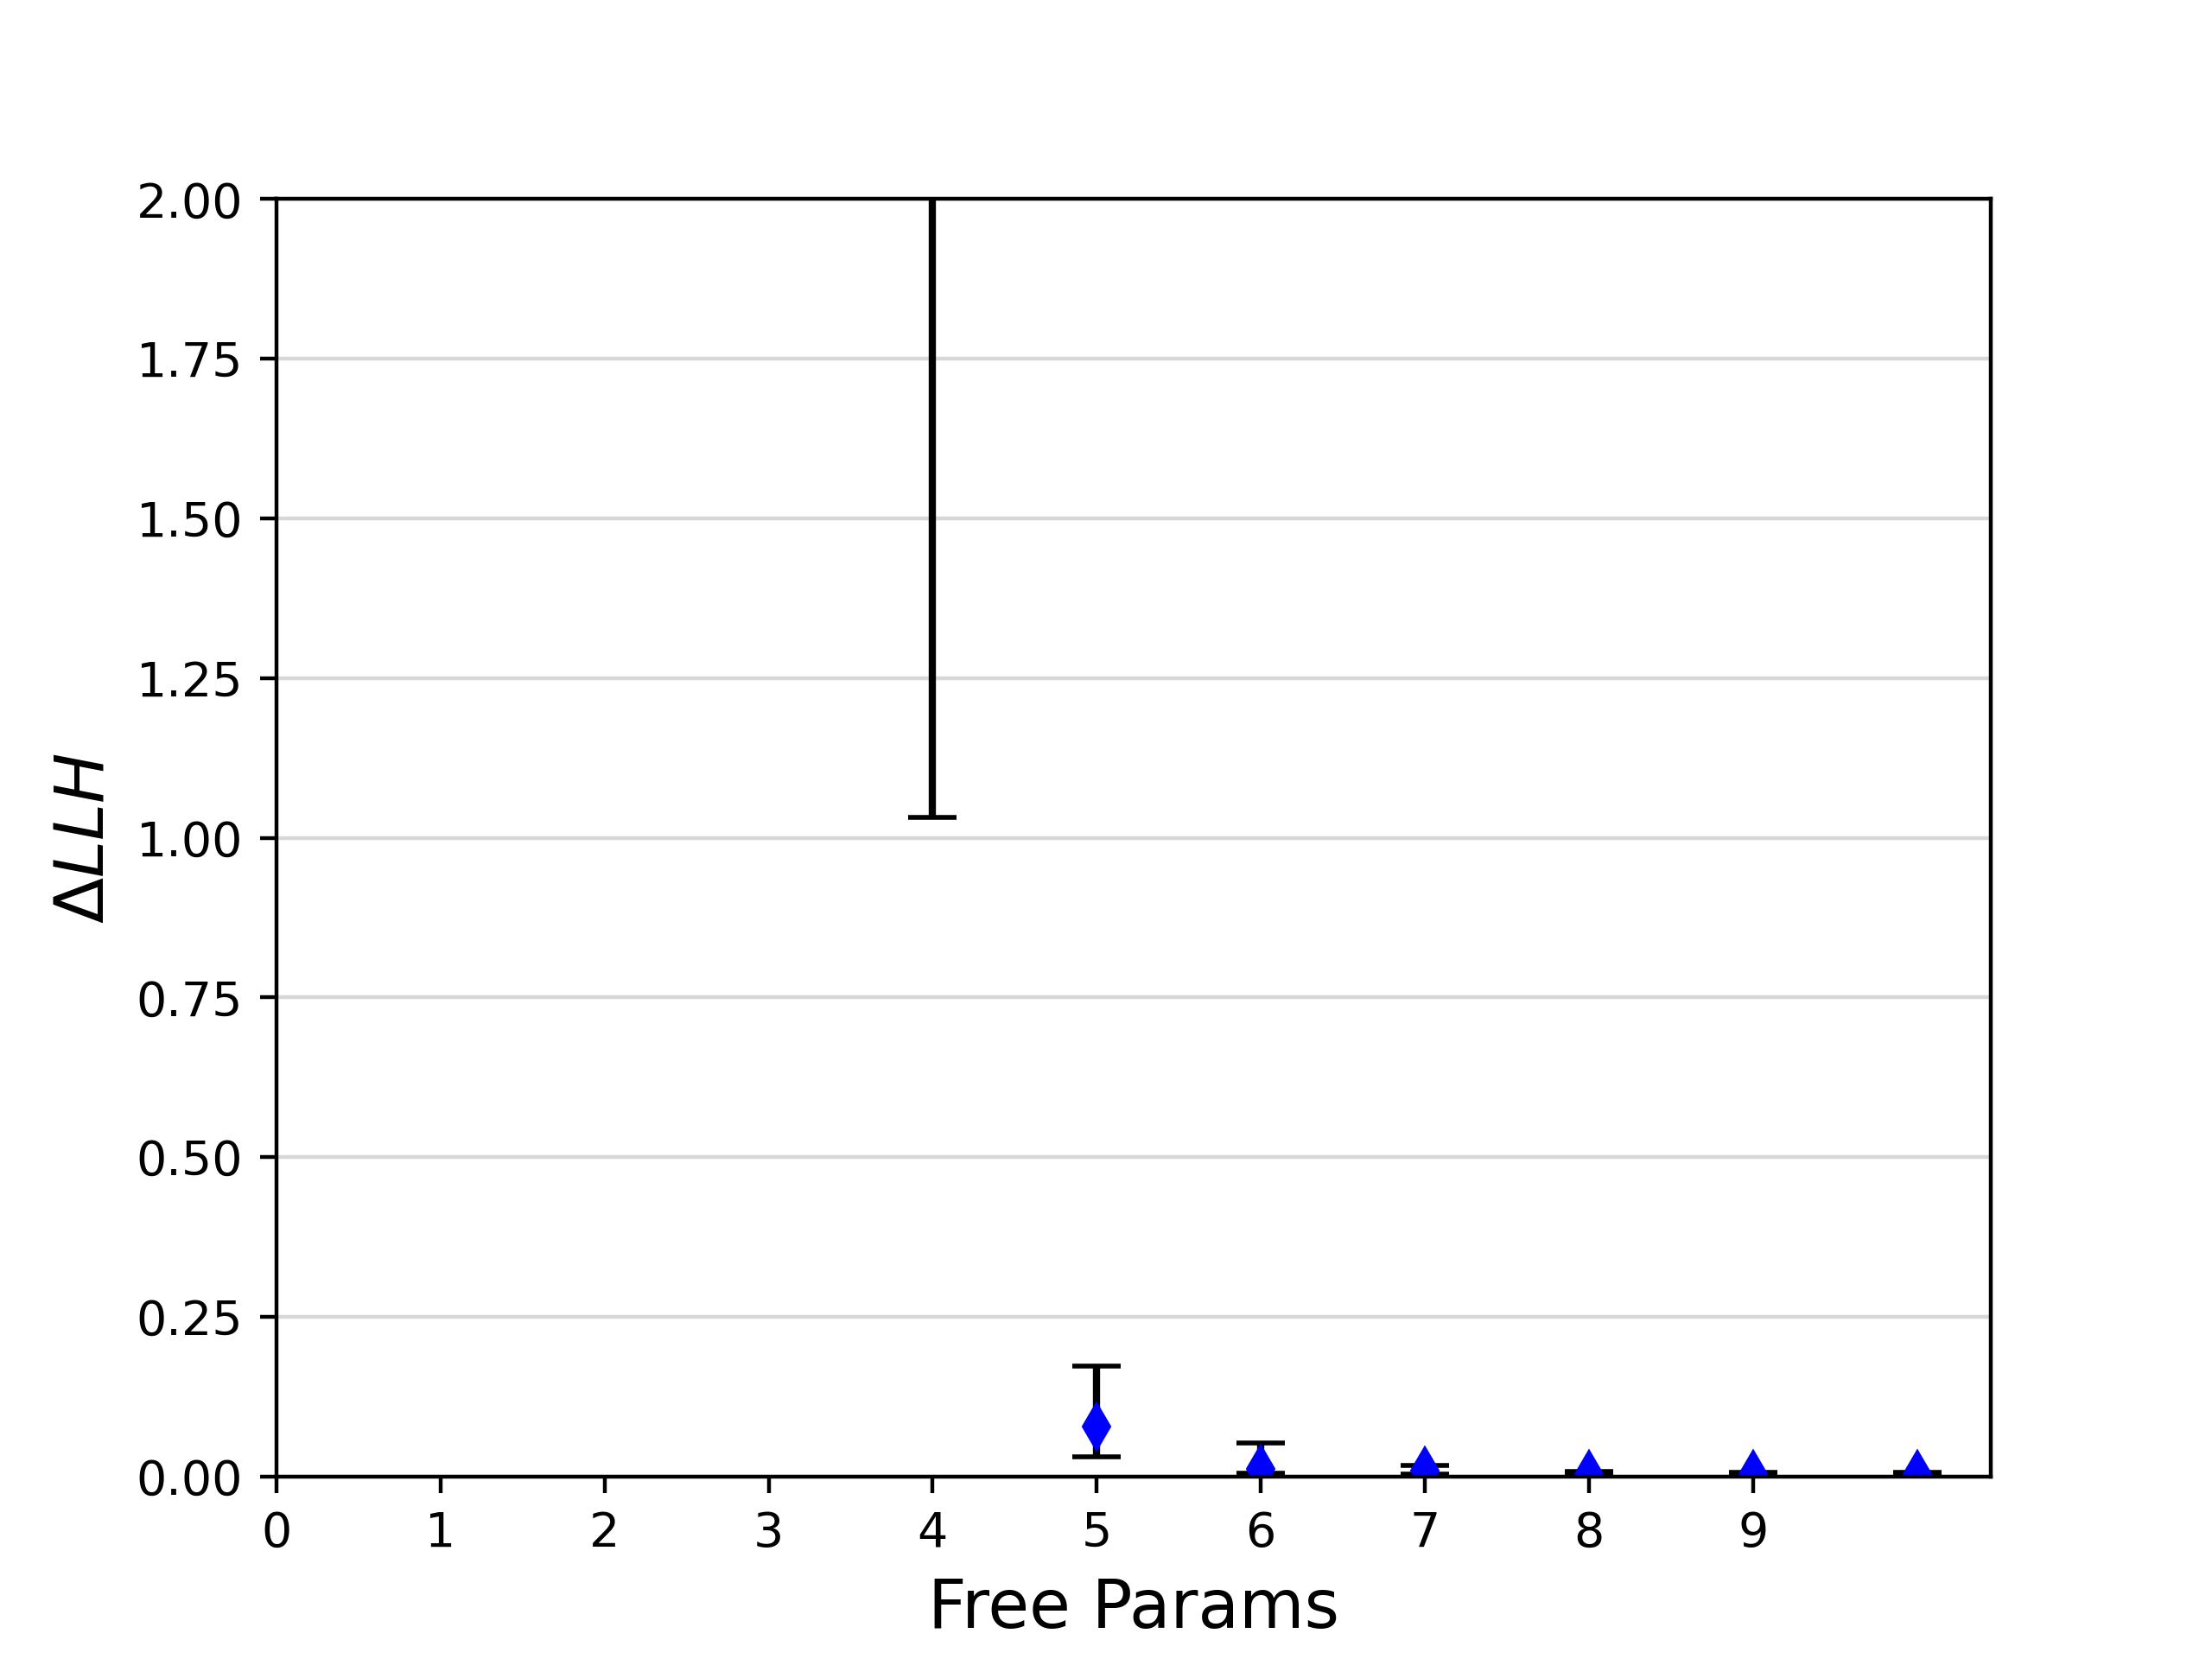
\includegraphics[width=0.45\linewidth]{figures/daemon/results_track.png}%
    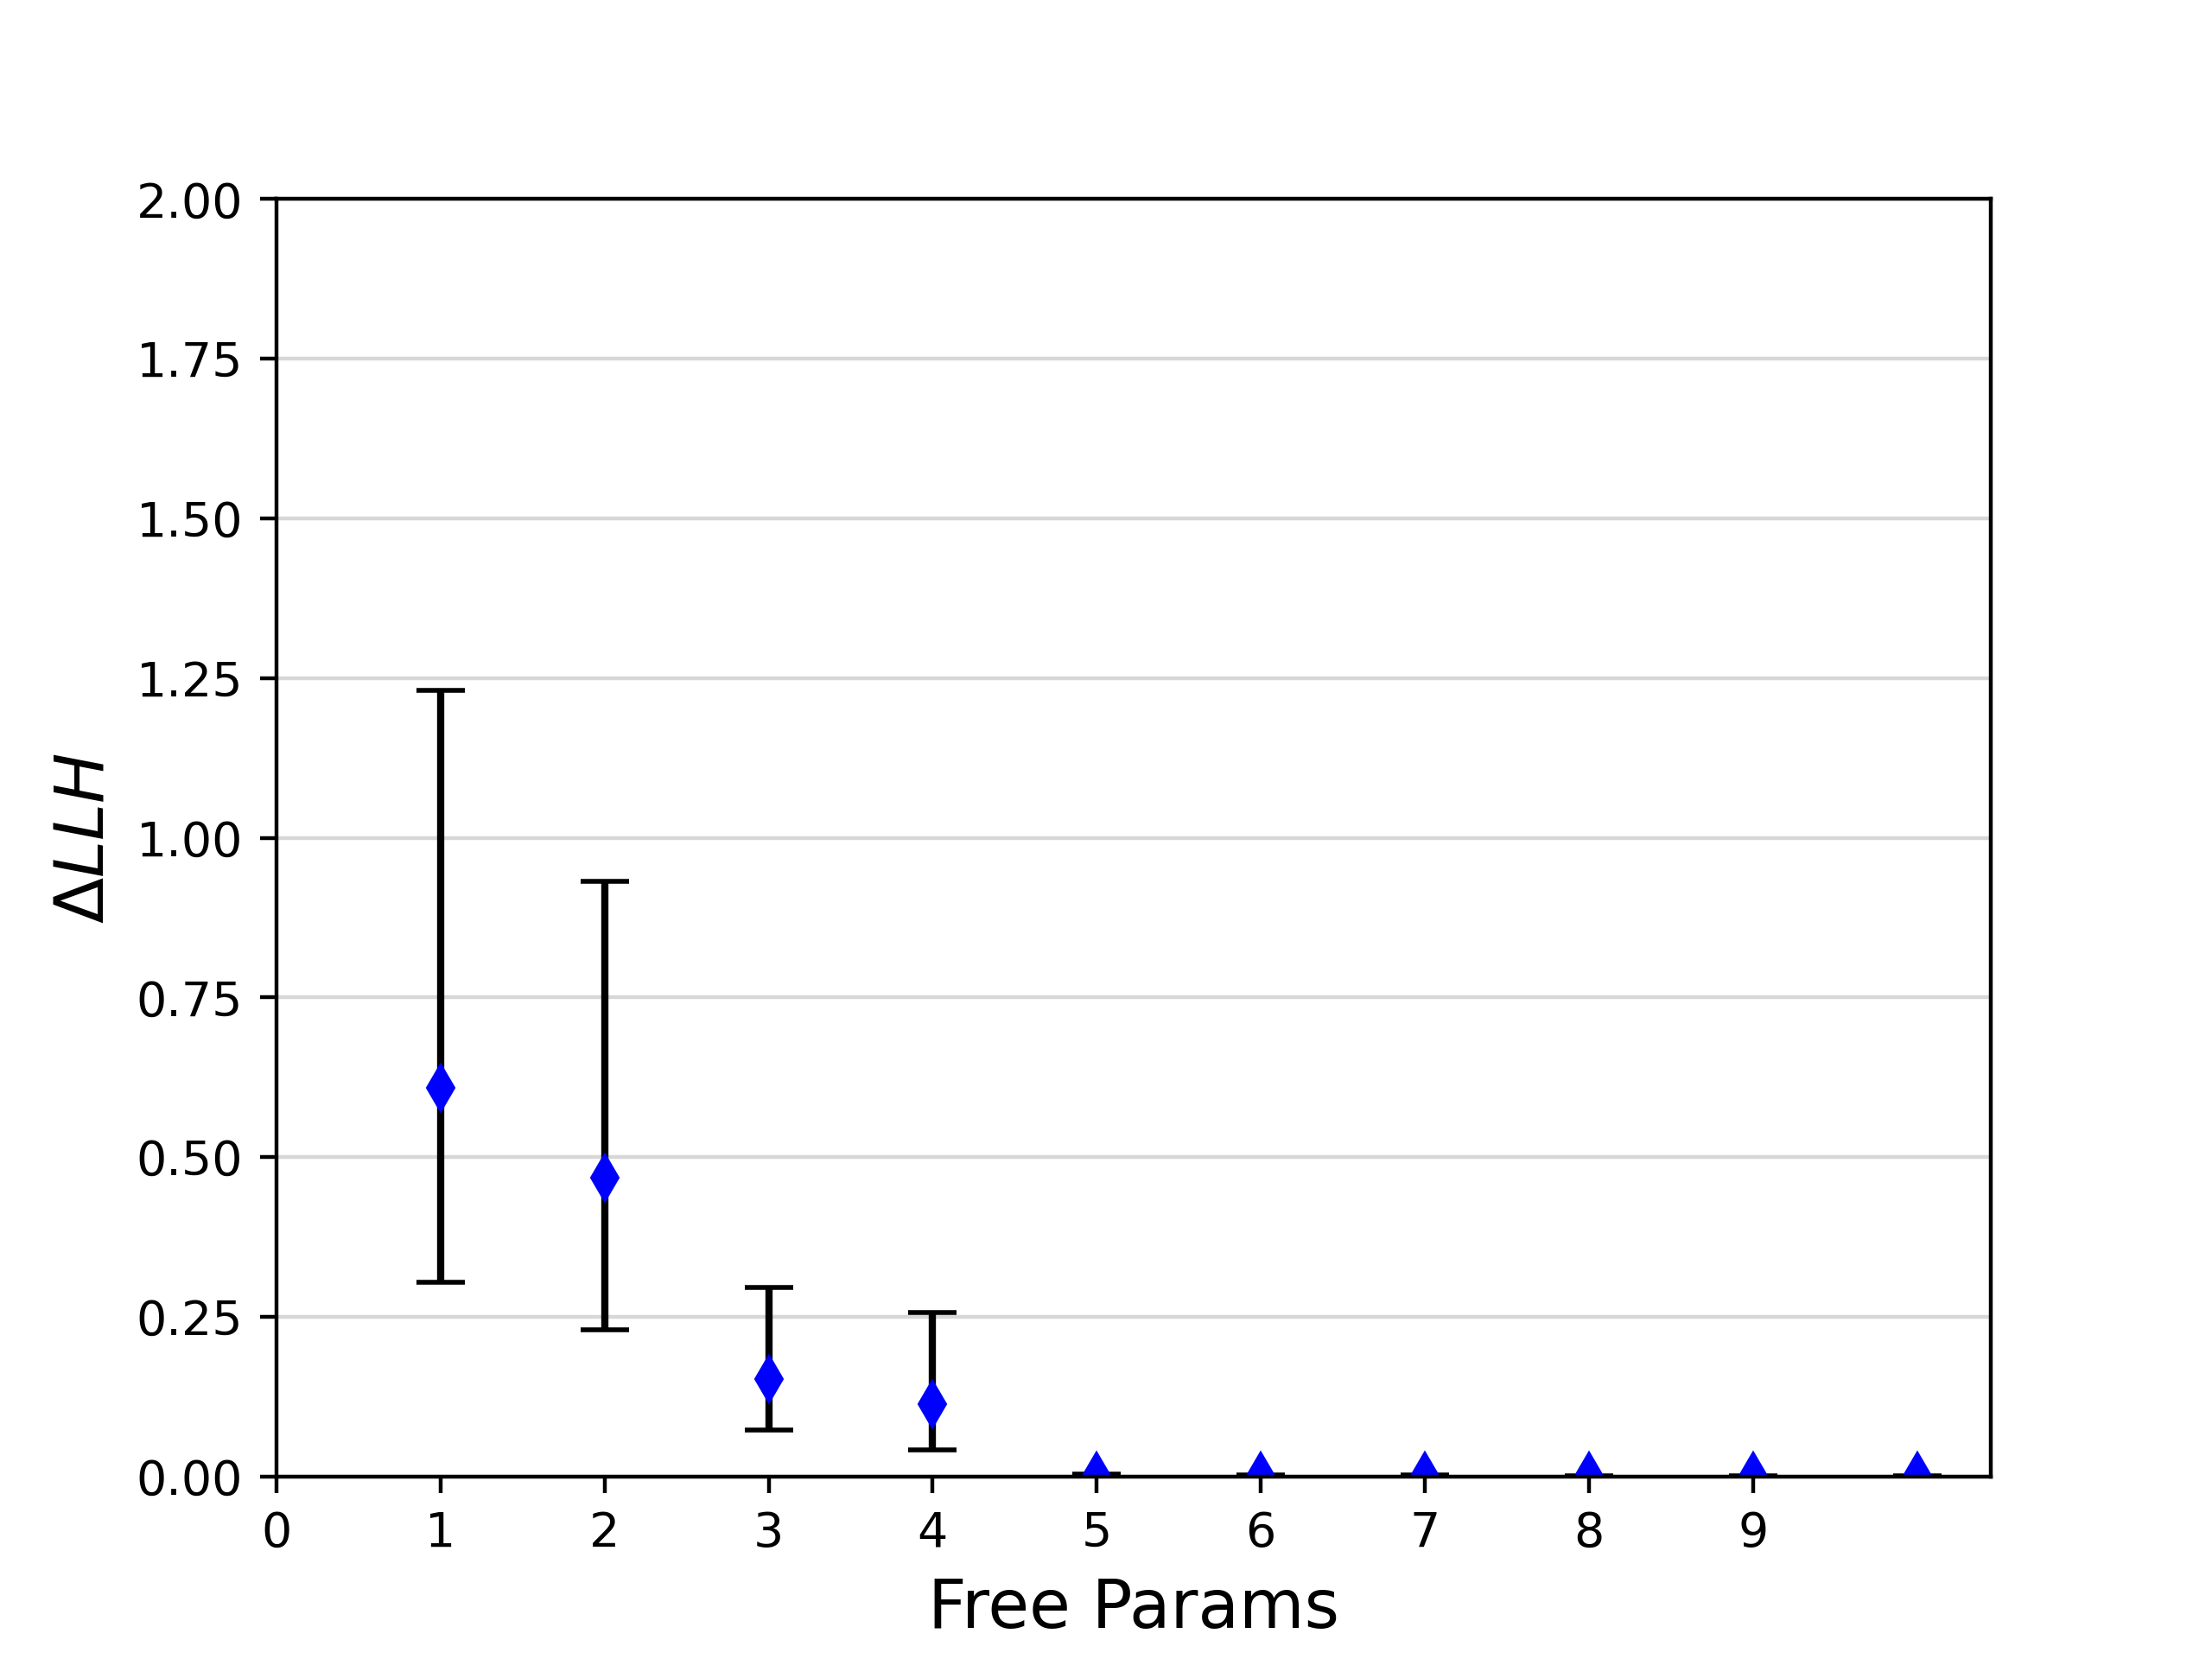
\includegraphics[width=0.45\linewidth]{figures/daemon/results.png}
    \caption{Fit accuracy as a function of free parameters used to a randomly sampled DaemonFlux expectation; tracks are shown on the left and cascades on the right}\label{fig:daemon_number}
\end{figure}   

\begin{table}
    \centering
    \rowcolors{2}{gray!25}{white}
    \begin{tabular}{l|cccccc}\rowcolor{blue!25}
        & $\theta_{24}$ [rad] & $\theta_{34}$ [rad] & $\Delta m_{41}^{2}$ [eV$^{2}$]  & 7 Params BF LLH & 14 Params BF LLH & ratio \\
        Null    & 0.0 & 0.0 & 0.0 & 4.6e-20 & 4.6e-20 & 1.0  \\
        Extreme & 2.13e-1 & 1.82e-1 & 4.5 & 20.76 & 19.54 & 1.06 \\
        Moderate & 2.13e-1 & 1.82e-1 & 1.0 & 13.42 & 12.62 & 1.06 \\
        Mild & 2.54 & 9.22e-2 & 1.0 & 3.19 & 3.00 & 1.06 \\
        Near-Null & 5.31e-2 & 3.16e-2 & 1.0 & 0.0216 & 0.0200 & 1.08
    \end{tabular}
    \caption{Results from fitting to an Asimov MC realization assuming different sterile neutrino hypotheses while using seven and fourteen DaemonFlux parameters.}\label{tab:daemonfluxfit}
\end{table}

\begin{figure}
    \centering
    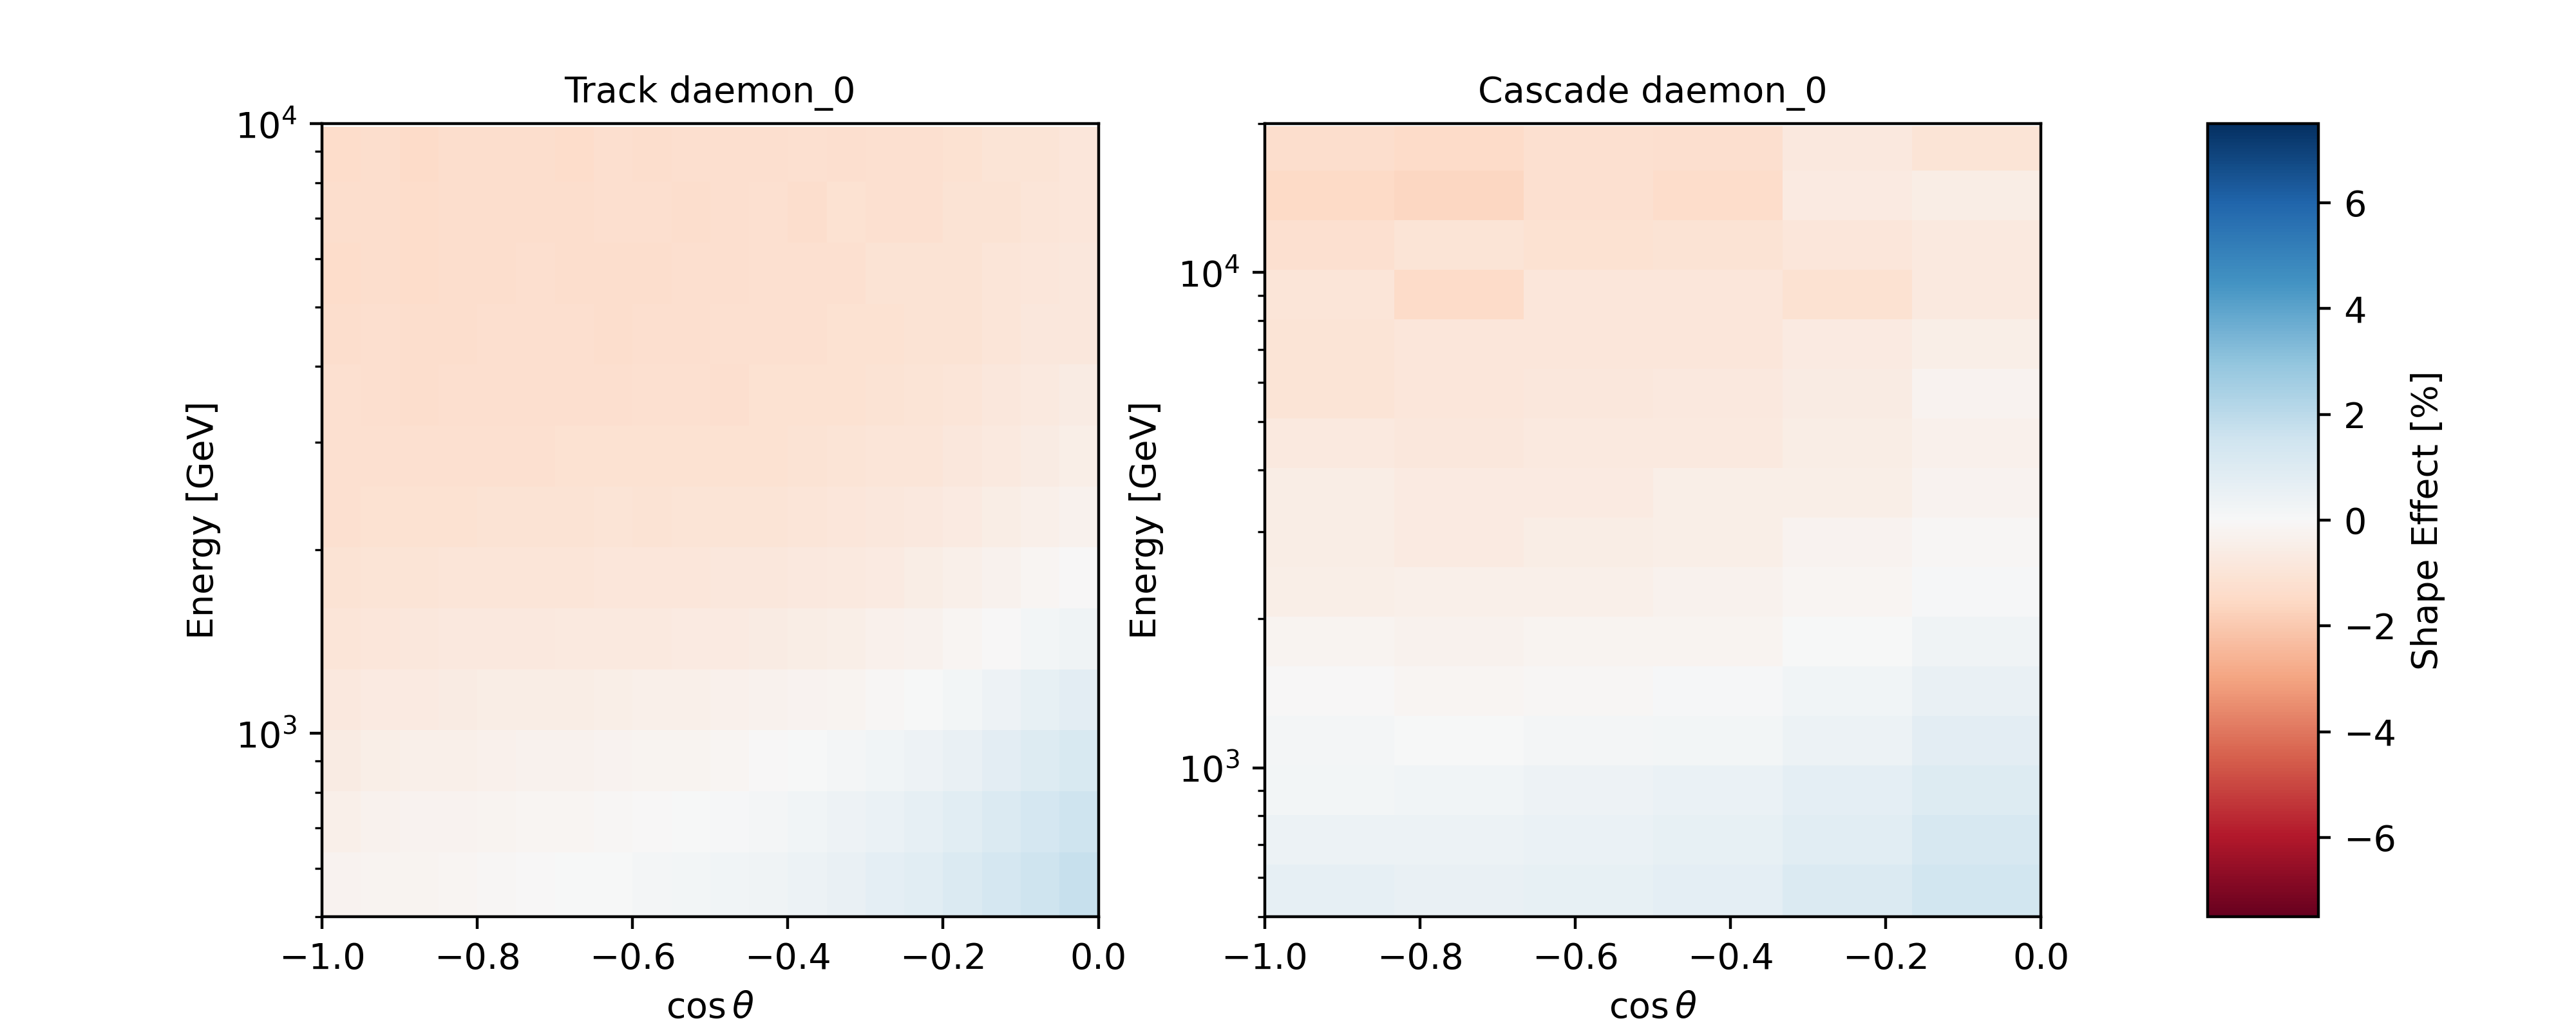
\includegraphics[width=0.45\linewidth]{figures/systematics/daemon_0.png}%
    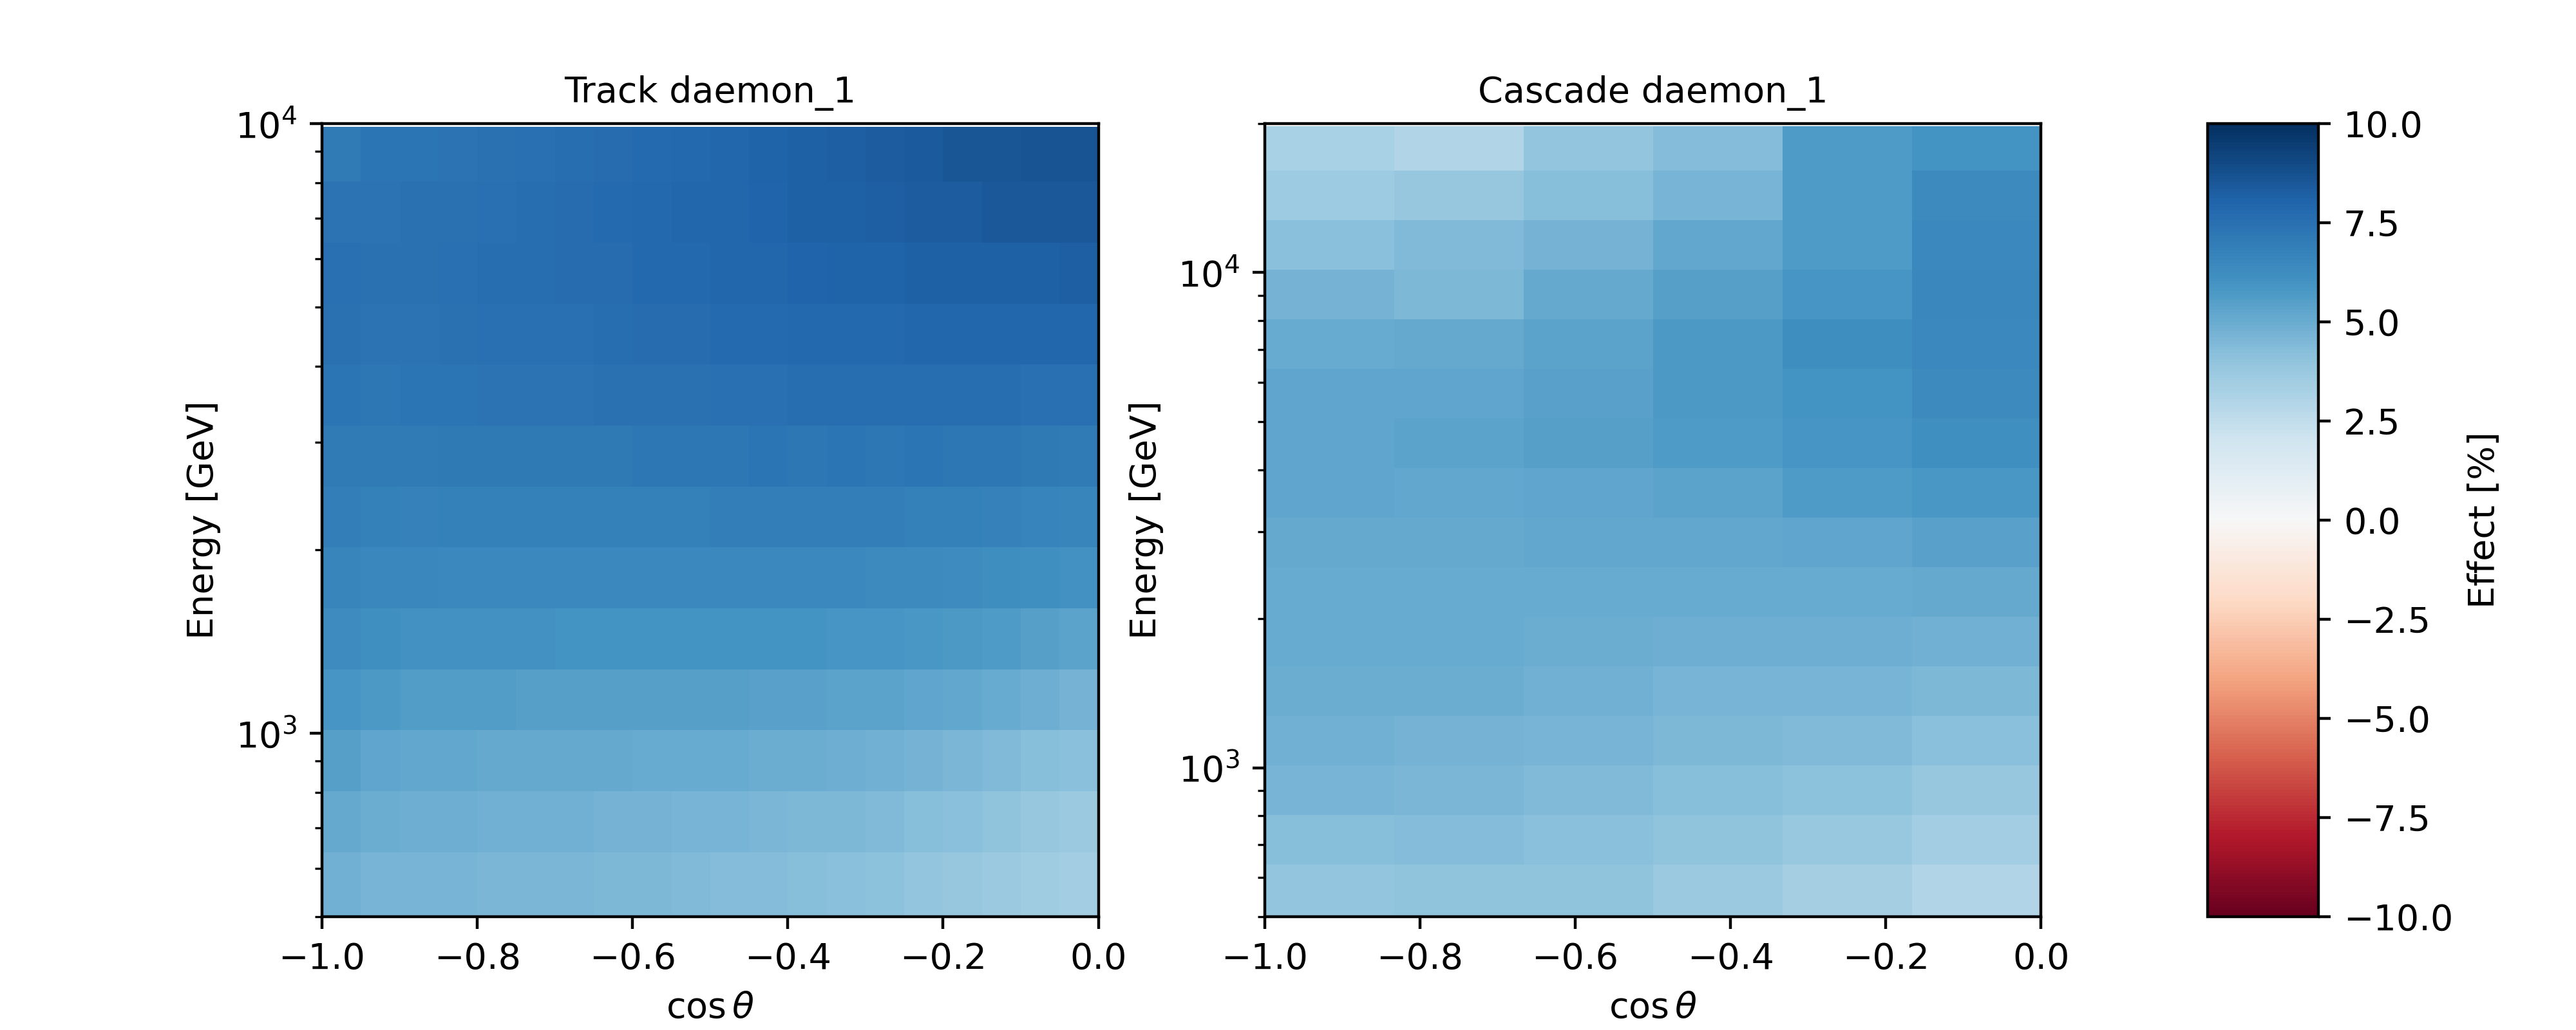
\includegraphics[width=0.45\linewidth]{figures/systematics/daemon_1.png}\\
    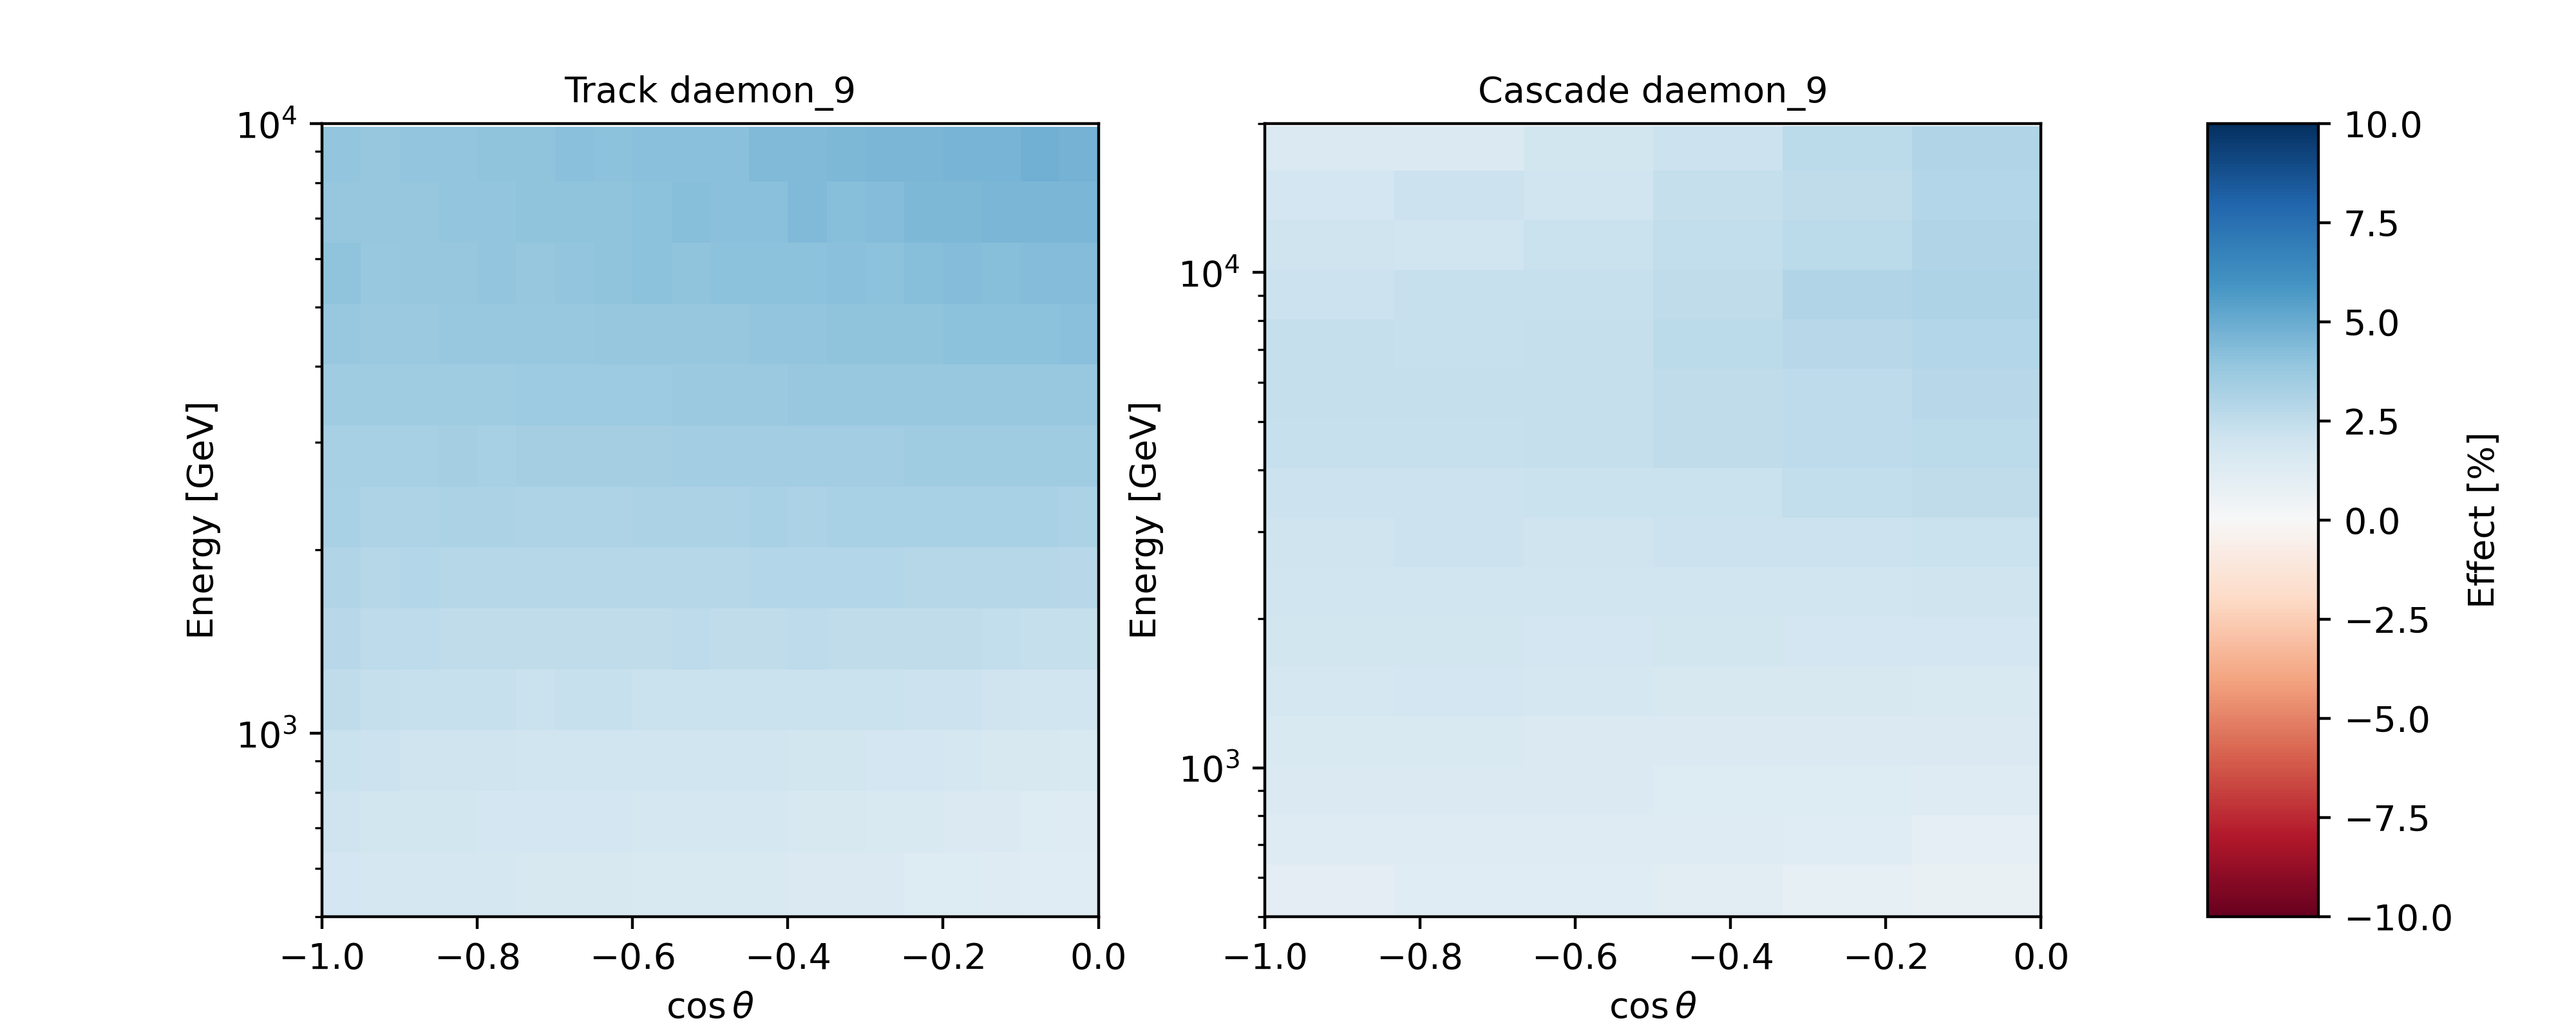
\includegraphics[width=0.45\linewidth]{figures/systematics/daemon_9.png}%
    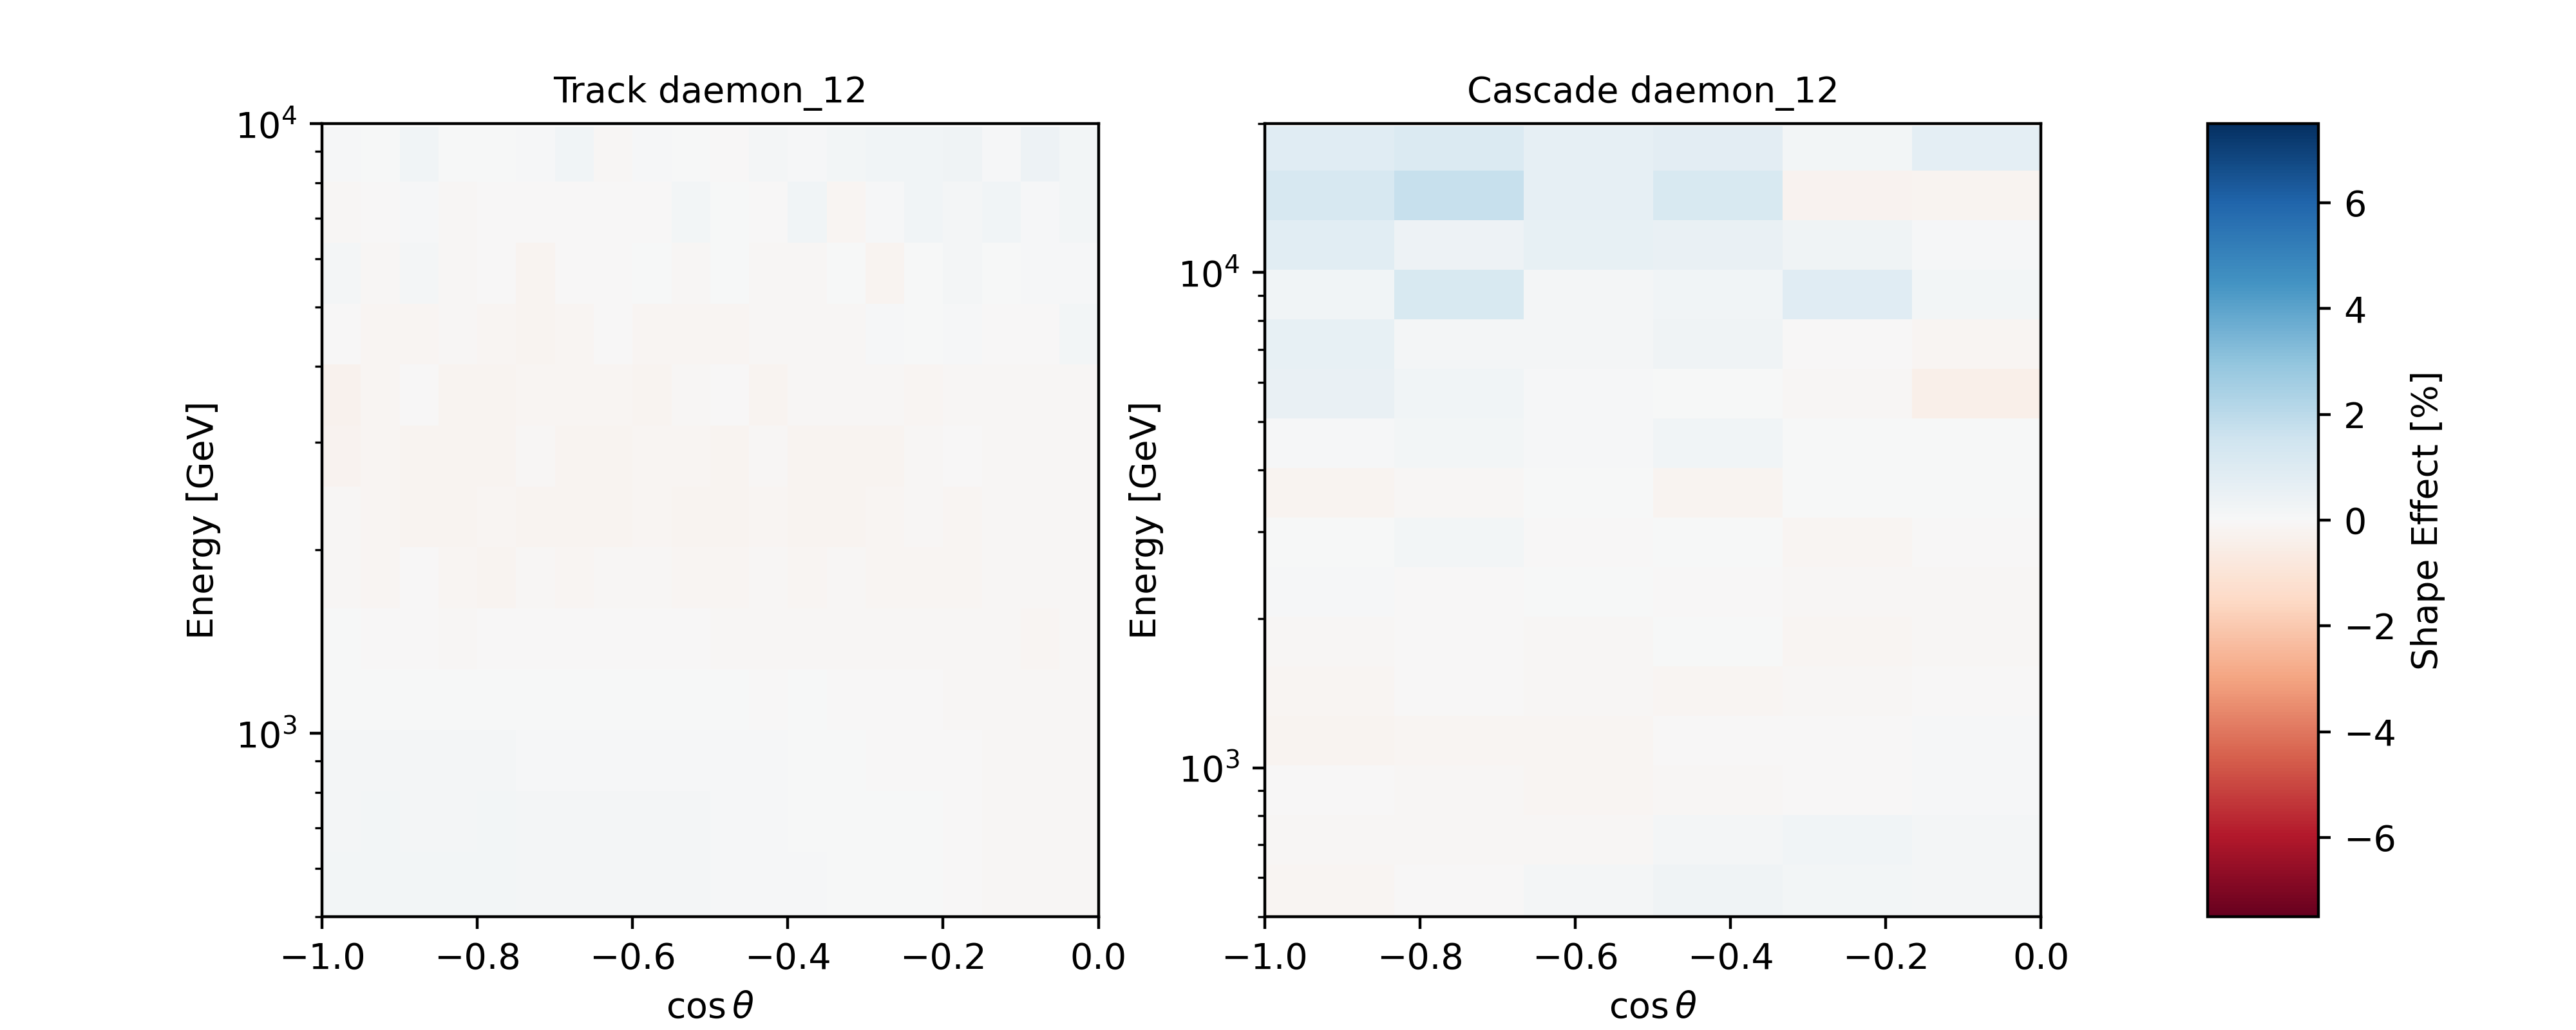
\includegraphics[width=0.45\linewidth]{figures/systematics/daemon_12.png}
    \caption{The shape-effect of perturbing four of the strongest uncorrelated DaemonFlux parameters for tracks and cascades.}\label{fig:daemon_analysis_one}
\end{figure}

\begin{figure}
    \centering
    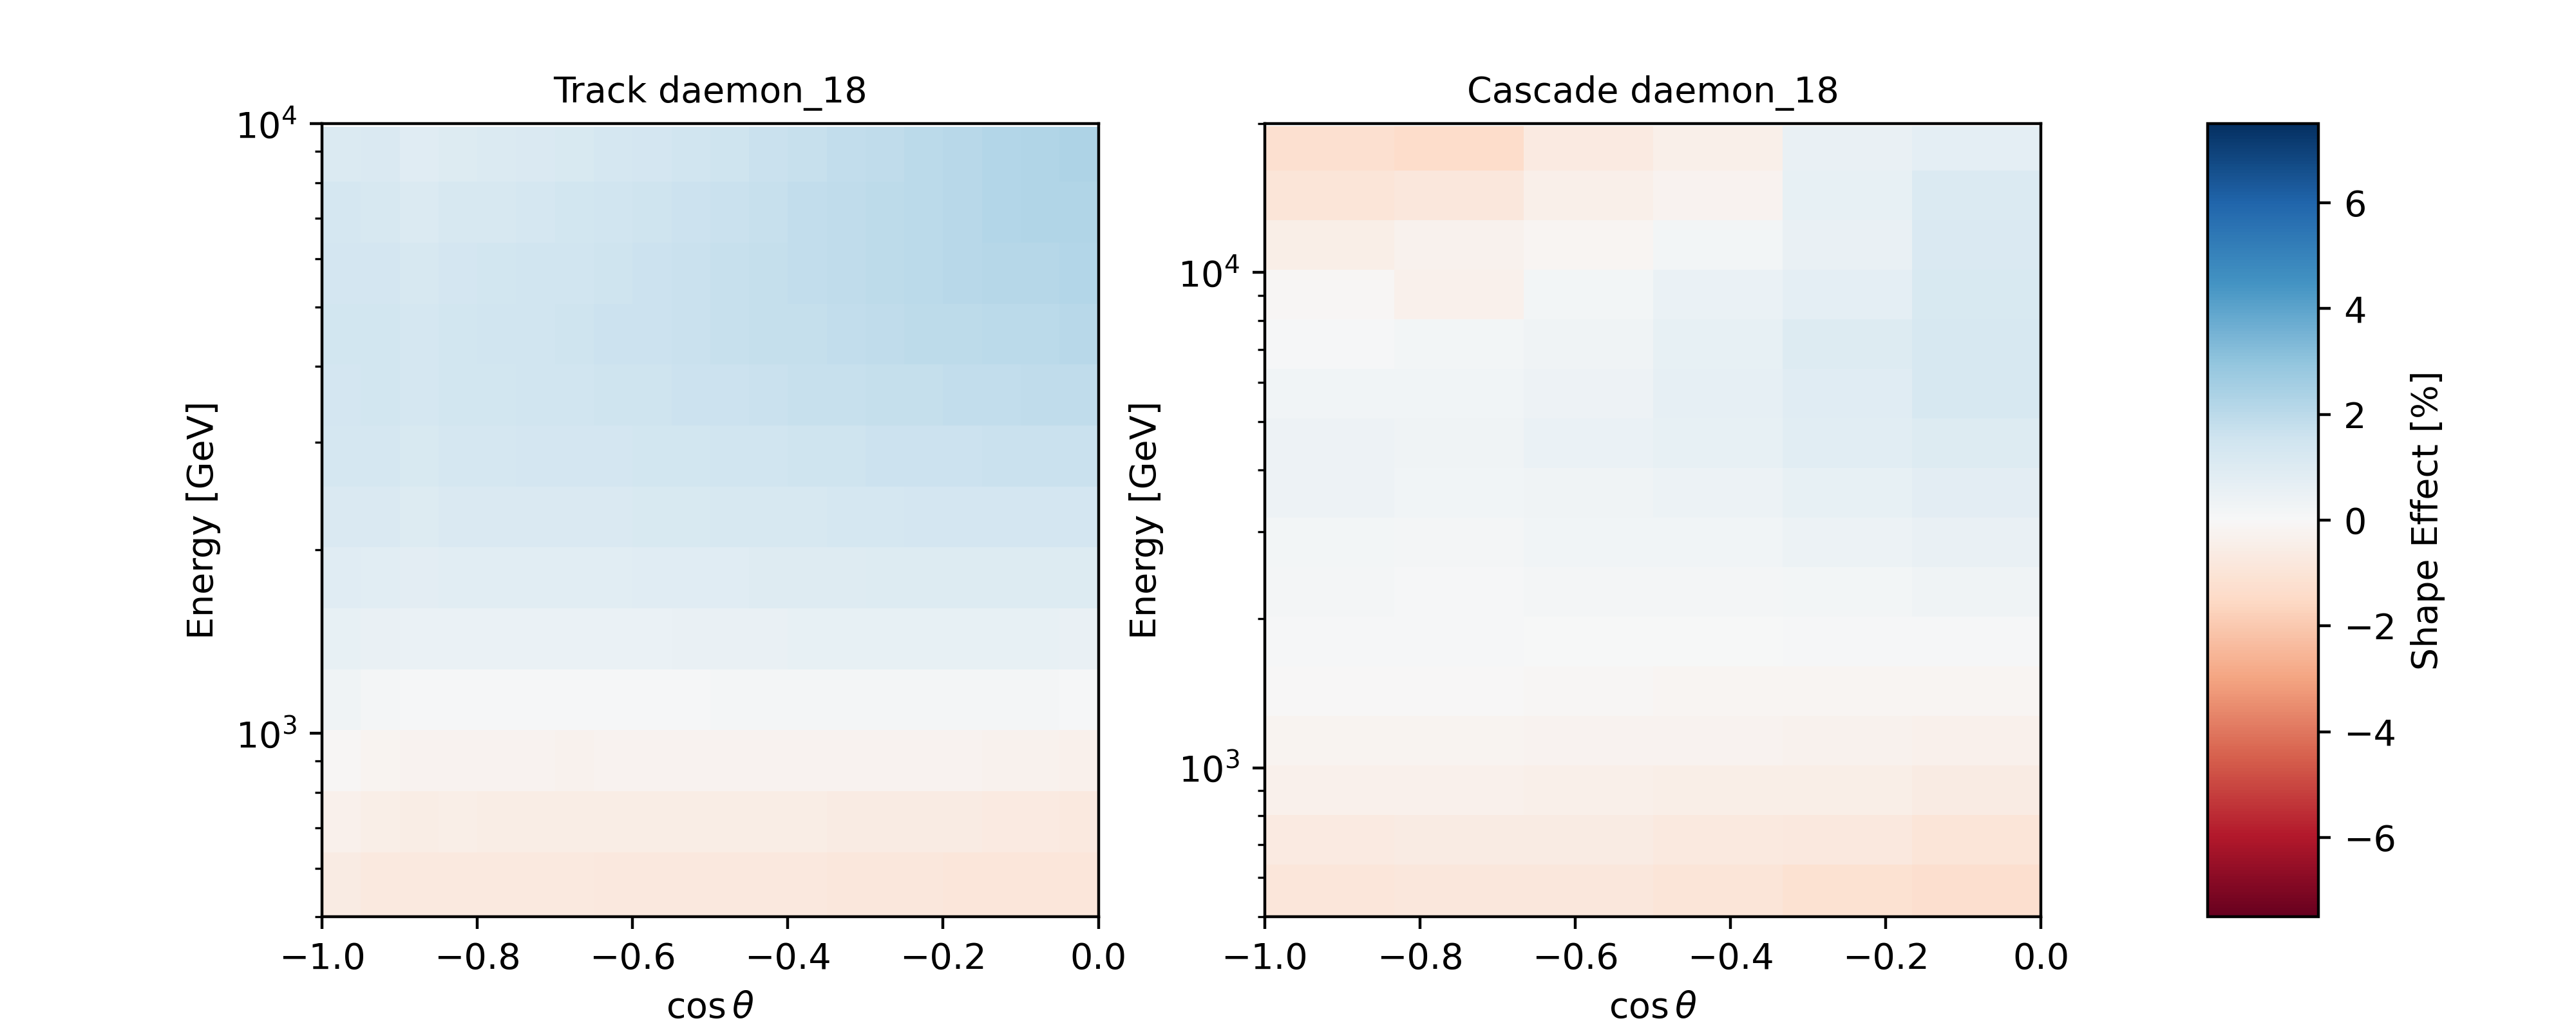
\includegraphics[width=0.45\linewidth]{figures/systematics/daemon_18.png}%
    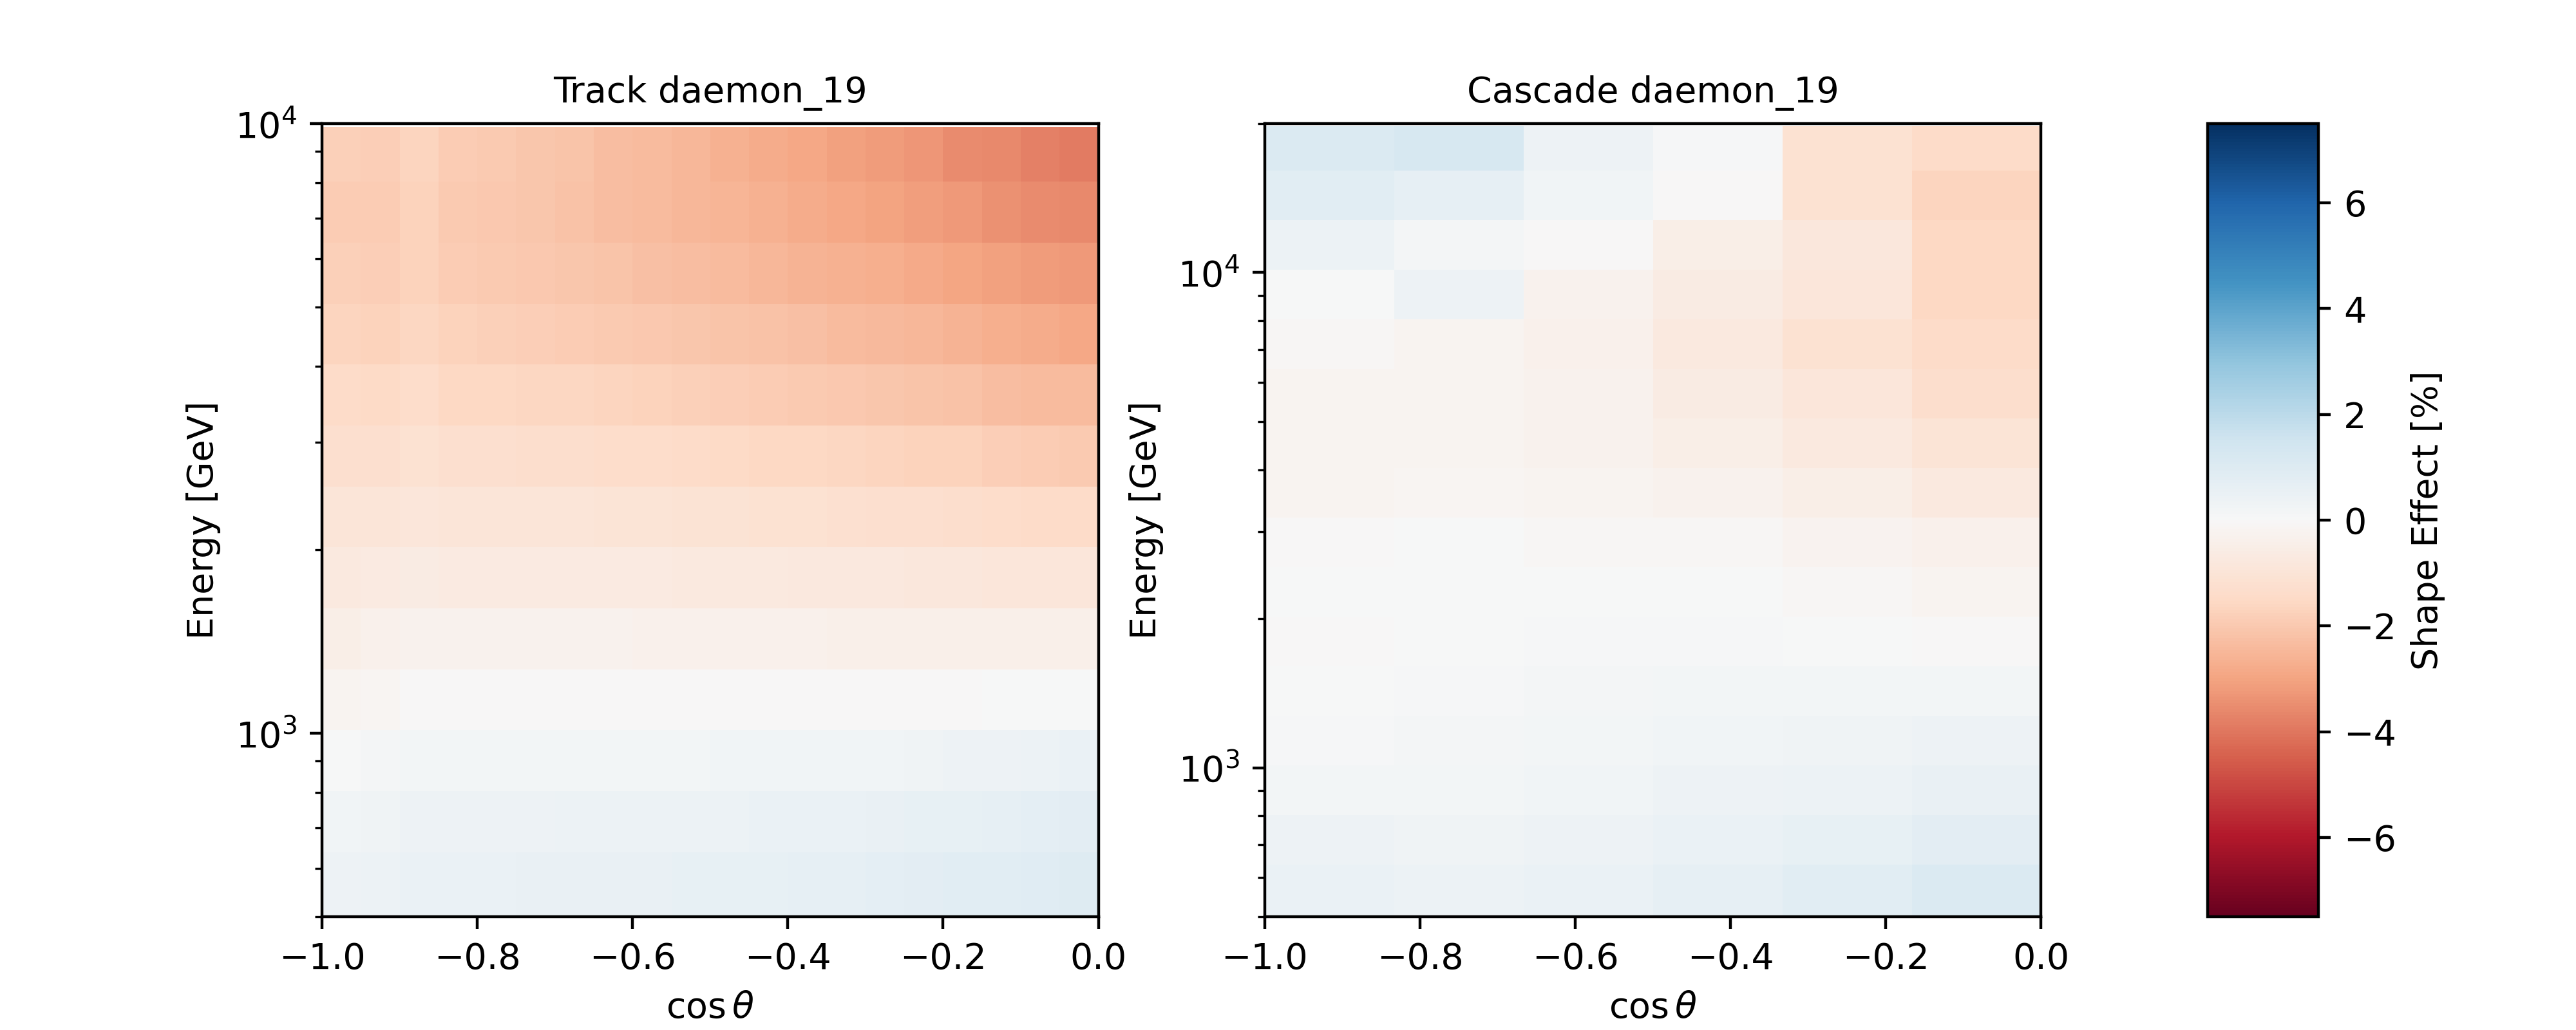
\includegraphics[width=0.45\linewidth]{figures/systematics/daemon_19.png}\\
    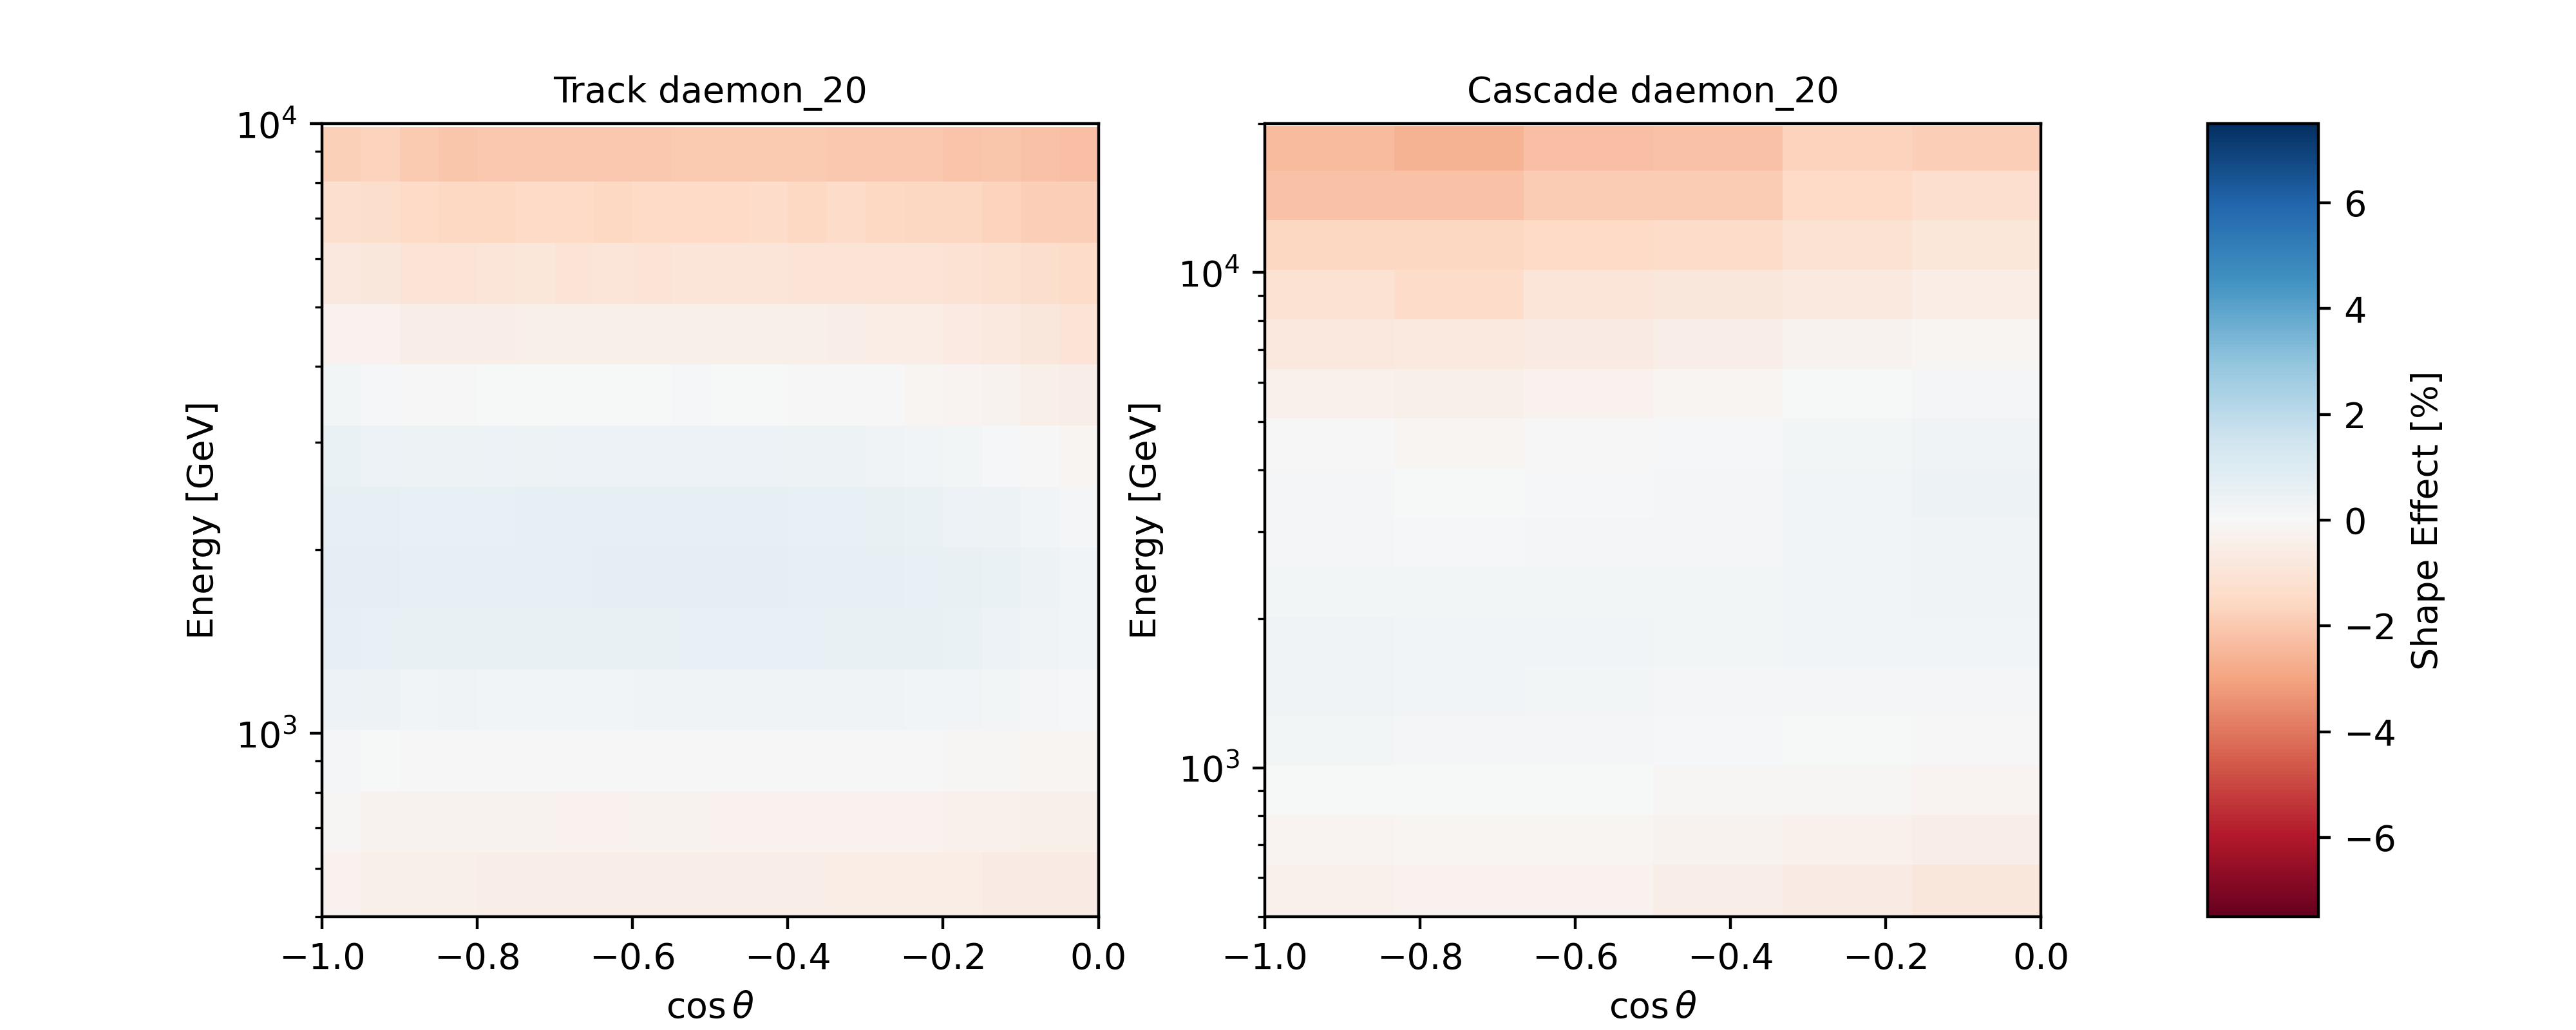
\includegraphics[width=0.45\linewidth]{figures/systematics/daemon_20.png}%
    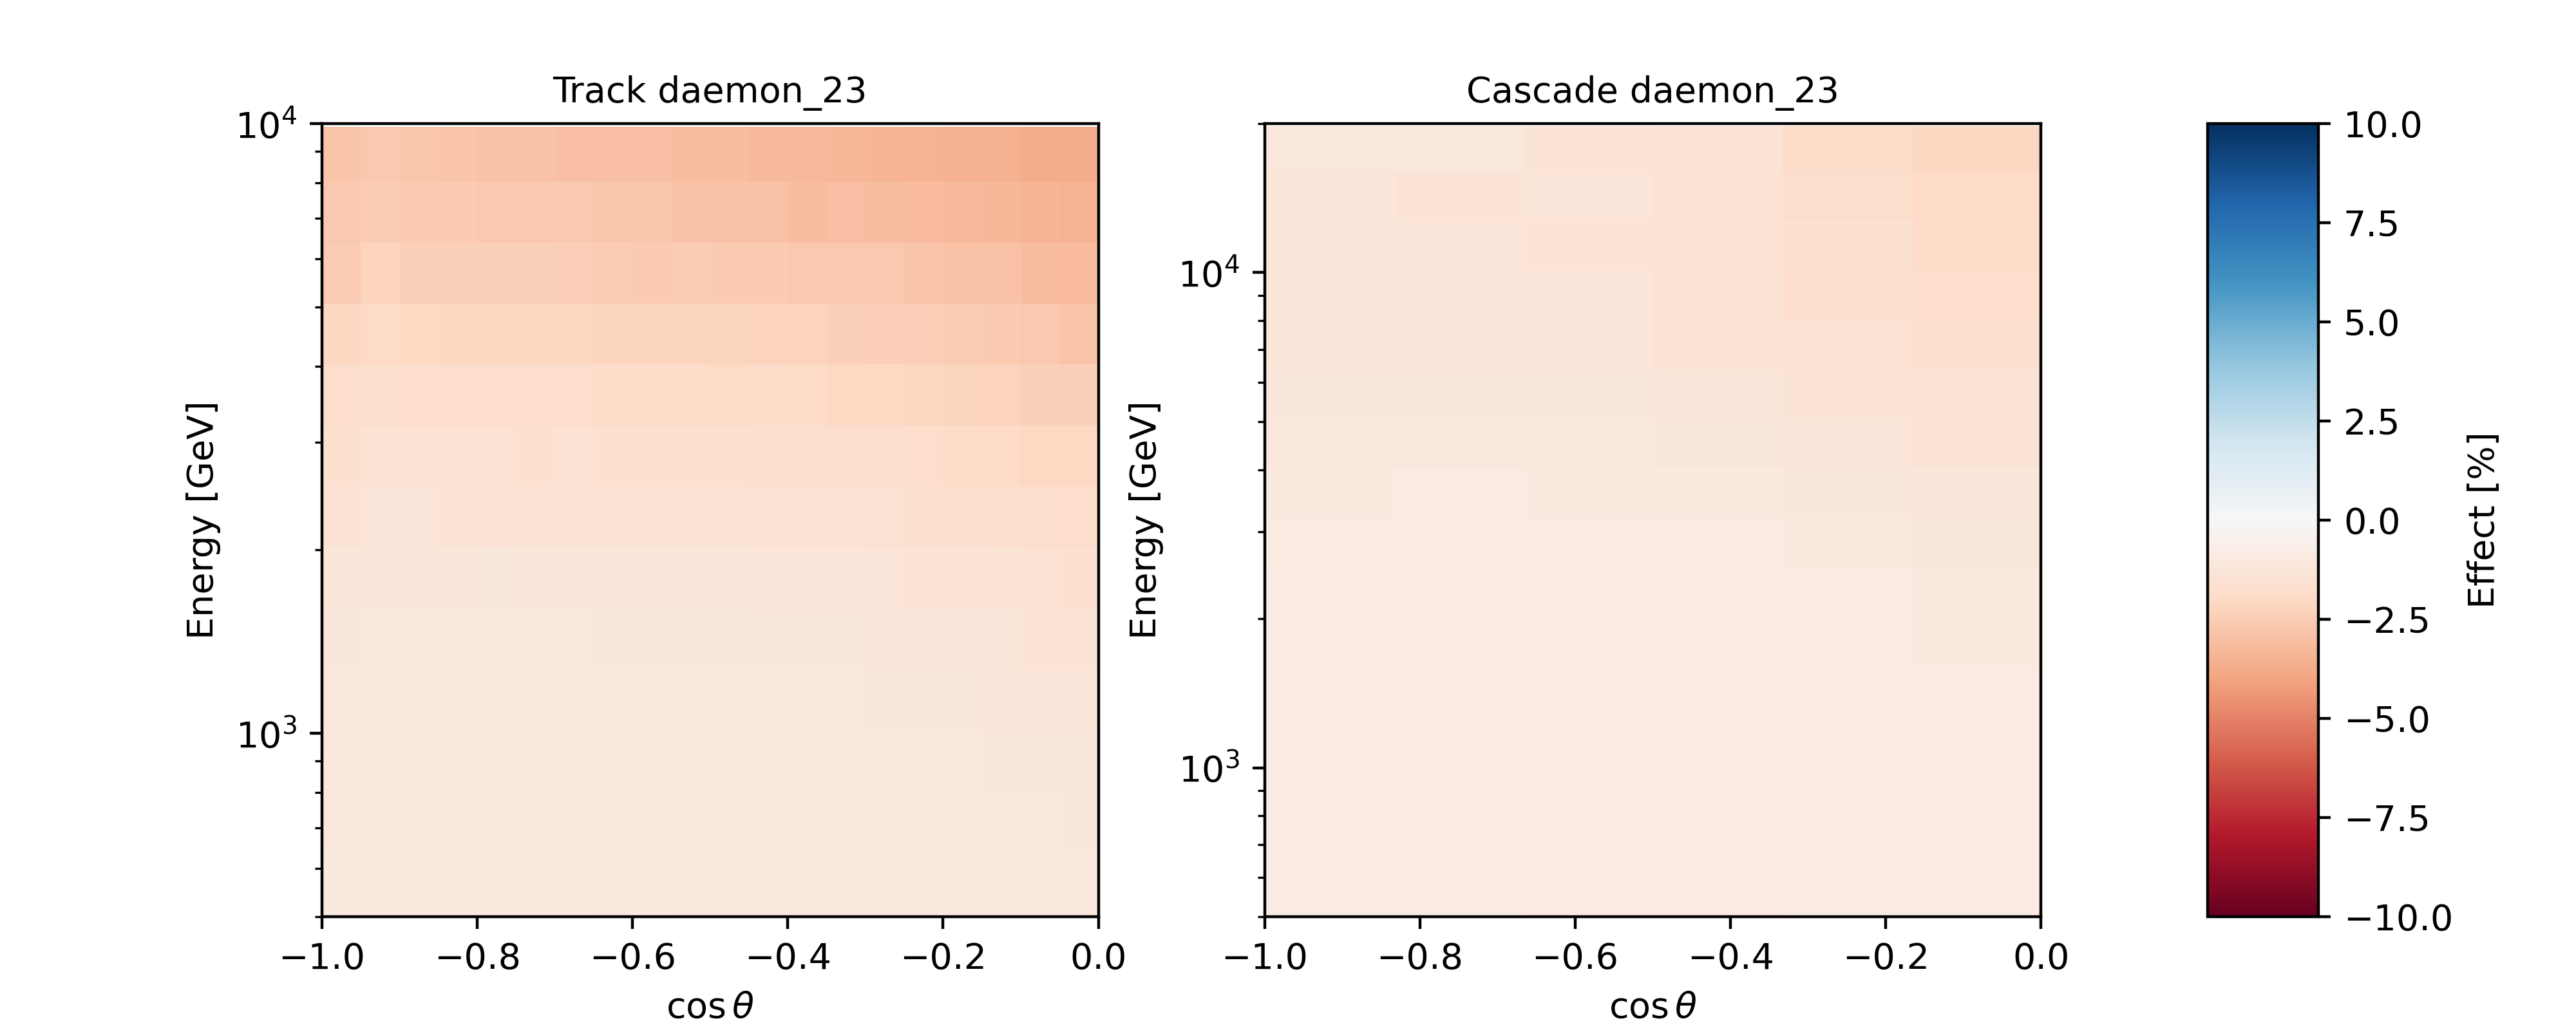
\includegraphics[width=0.45\linewidth]{figures/systematics/daemon_23.png}
    \caption{The shape-effect of perturbing four more of the strongest uncorrelated DaemonFlux parameters for tracks and cascades.}\label{fig:daemon_analysis_two}
\end{figure}

\subsection{Atmospheric Density}

During air shower evolution, the delicate balance between kaon production, re-interaction, and decay heavily influence the energy spectrum of the resulting neutrinos. 
The local atmospheric conditions of the temperature, density, and pressure all influence this balance; an effect that has previously been studied in the neutrino spectrum by IceCube~\cite{heix2019seasonal,abbasi2023observation}. 
We incorporate an uncertainty on the atmospheric density by perturbing the Earth's atmospheric temperature within the ranges specified by NASA's Atmospheric InfraRed Sounder (AIRS) \textbf{CITE} satellite data. 
This satellite provides an open-source dataset for the temperature profile of the atmospheric as a function of atmospheric depth and location. 
We evaluate the variation in the temperature of the atmosphere over a whole year in a $1^{\circ}\times1^{\circ}$ grid across the Earth's surface. 
The standard deviation of the predictions from all models are then calculated as functions of zenith and energy. 
This standard deviation is shown for muon and electron neutrinos in Figure~\ref{fig:airs_raw}.

\begin{figure}
    \centering
    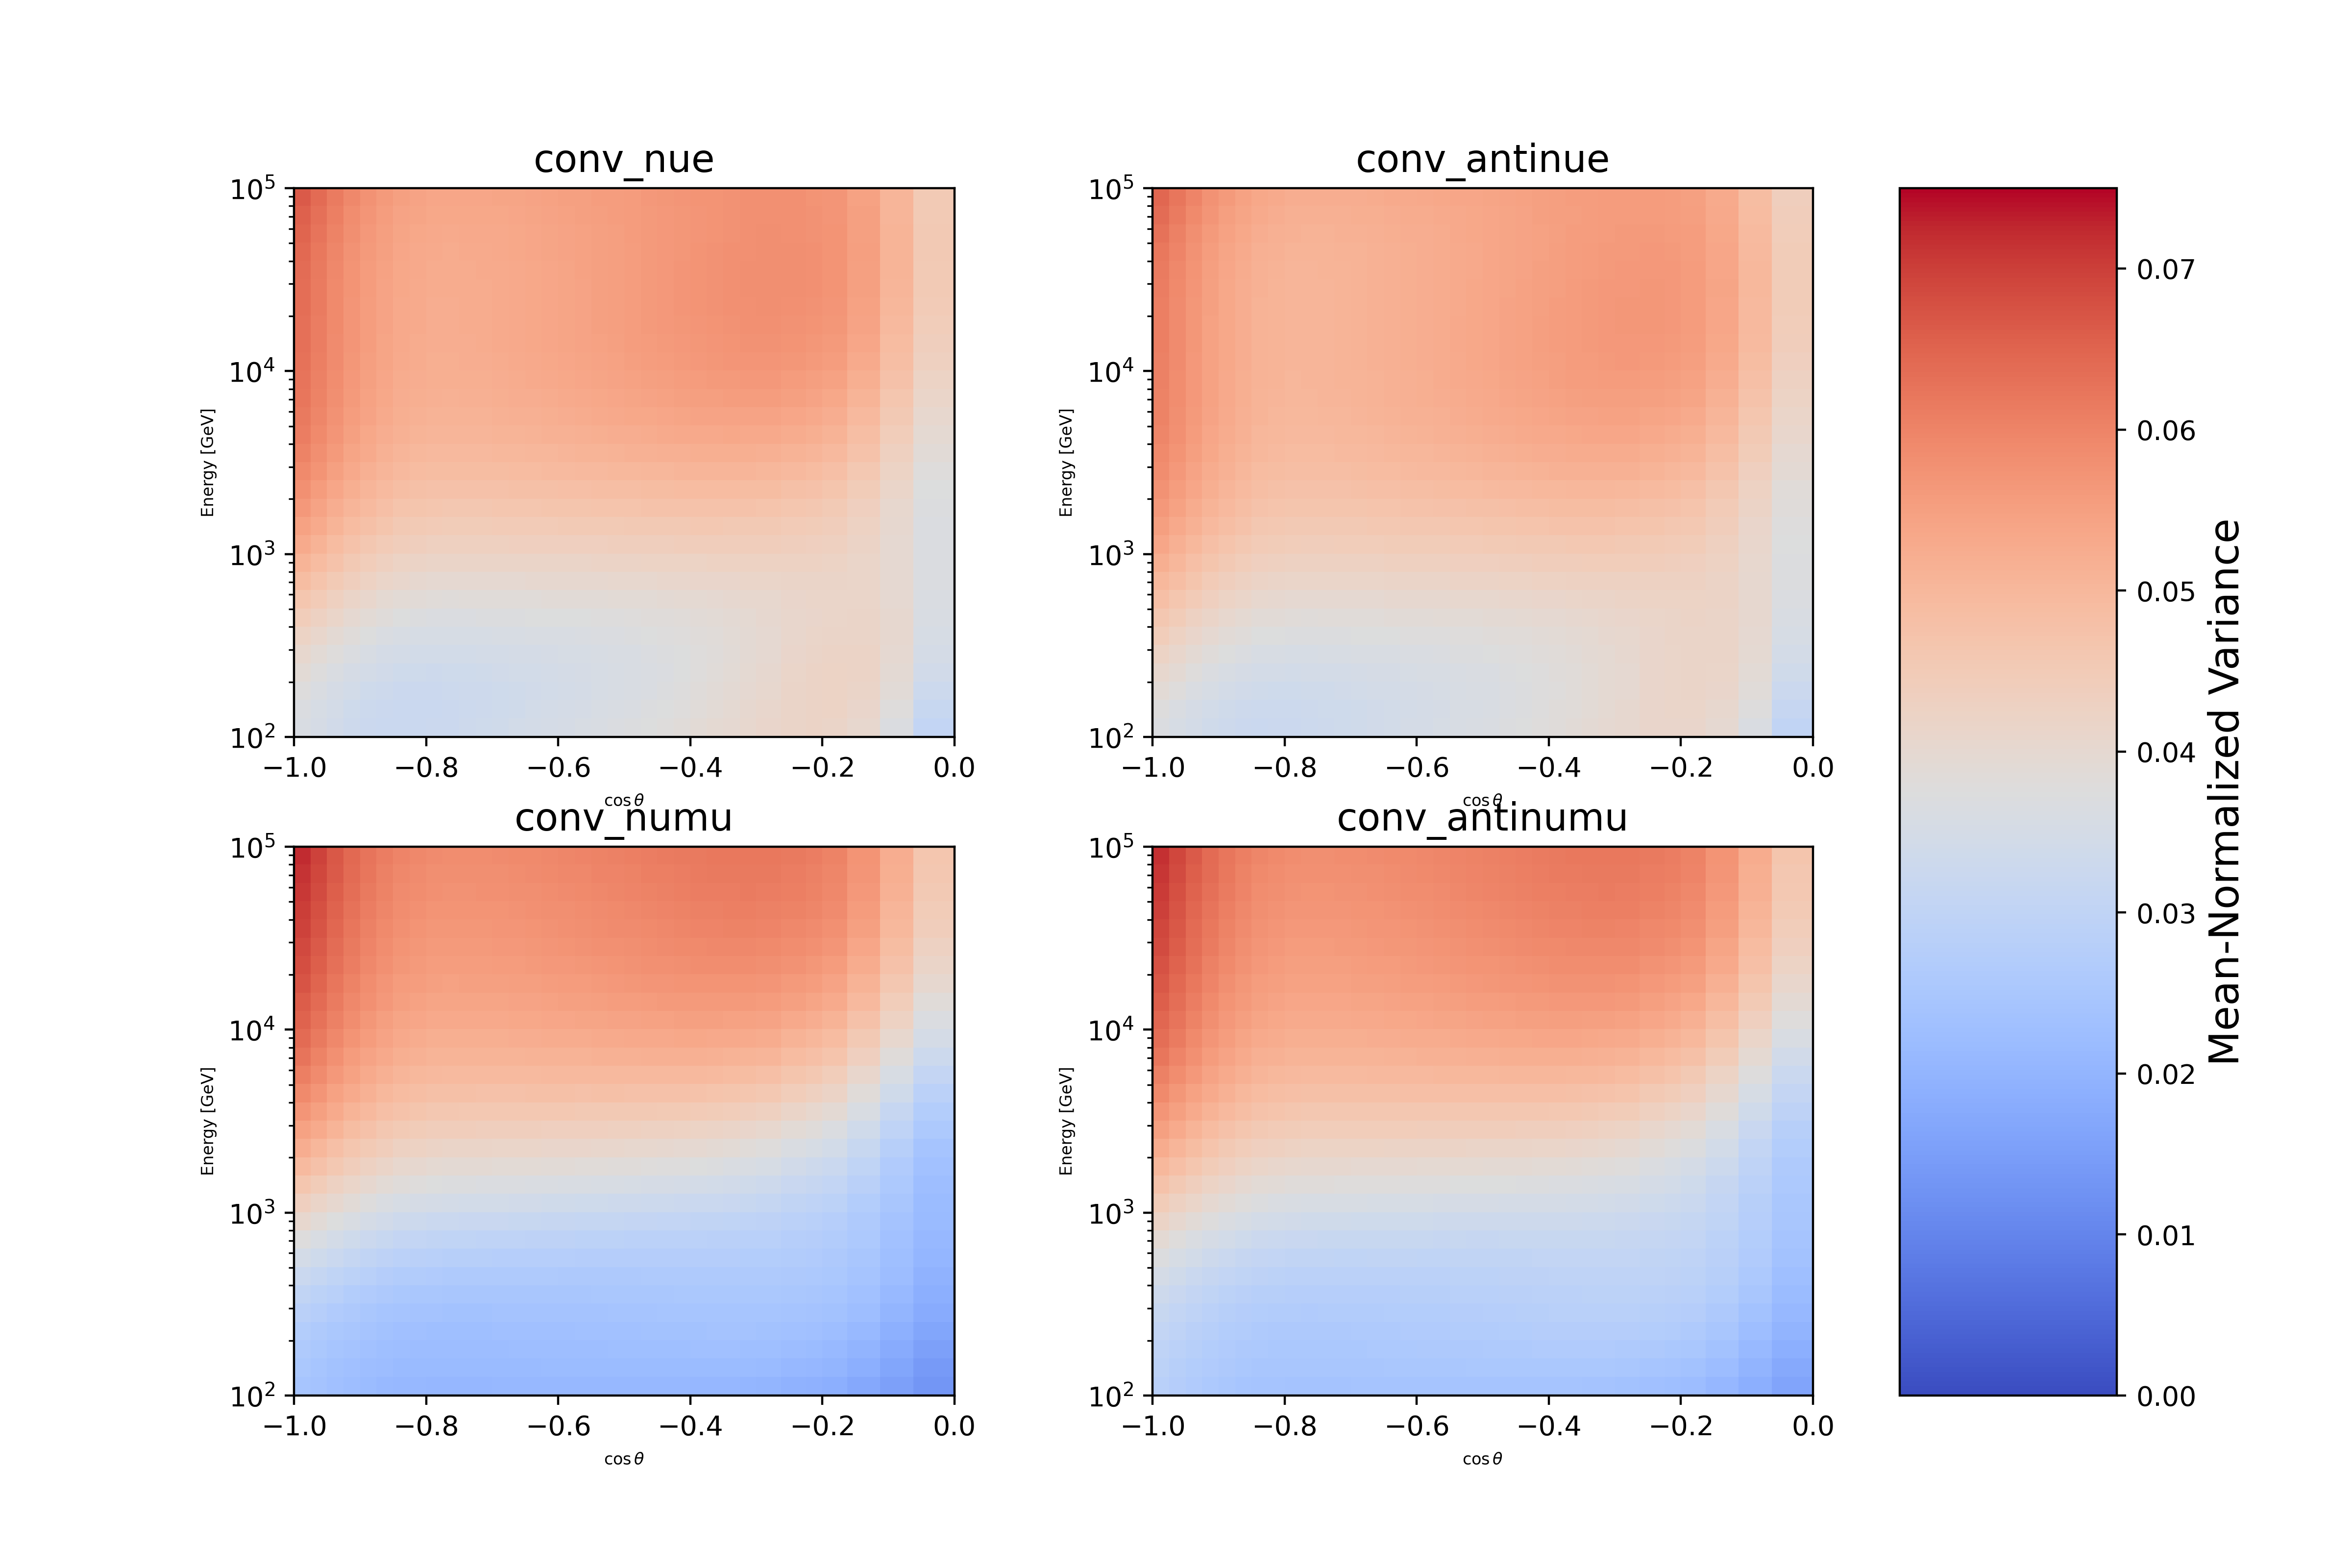
\includegraphics[width=0.8\linewidth]{figures/airs_grid_var.png}
    \caption{The variance in predicted atmospheric models for various neutrino fluxes before nuSQuIDS propagation. From the top left, going clockwise, $\nu_{e}$, $\bar{\nu}_{e}$, $\nu_{\mu}$, and $\bar{\nu}_{\mu}$. }\label{fig:airs_raw}
\end{figure}

This is then used as the atmospheric density uncertainty after being forced through zero near $\cos\theta_{z}=-0.7$ to account for the temperature offset between the Northern and Southern hemispheres. 
Figure~\ref{fig:airs_grid} shows the effect on neutrino fluxes after forcing it through zero at the equator.
This effect is calculated as a gradient effecting the neutrino flux, and it is then evolved through the Earth for each sterile neutrino model to propagate the effects into other neutrino flavors. 
The effects of this nuisance parameter, and this source of systematic uncertainty, is shown in Figure~\ref{fig:airs_reco}.

The 1976 United States Standard atmosphere~\cite{united1976u} was also used as a baseline for cross-checks, and it was found to lie within the allowed envelope. 

\begin{figure}
    \centering
    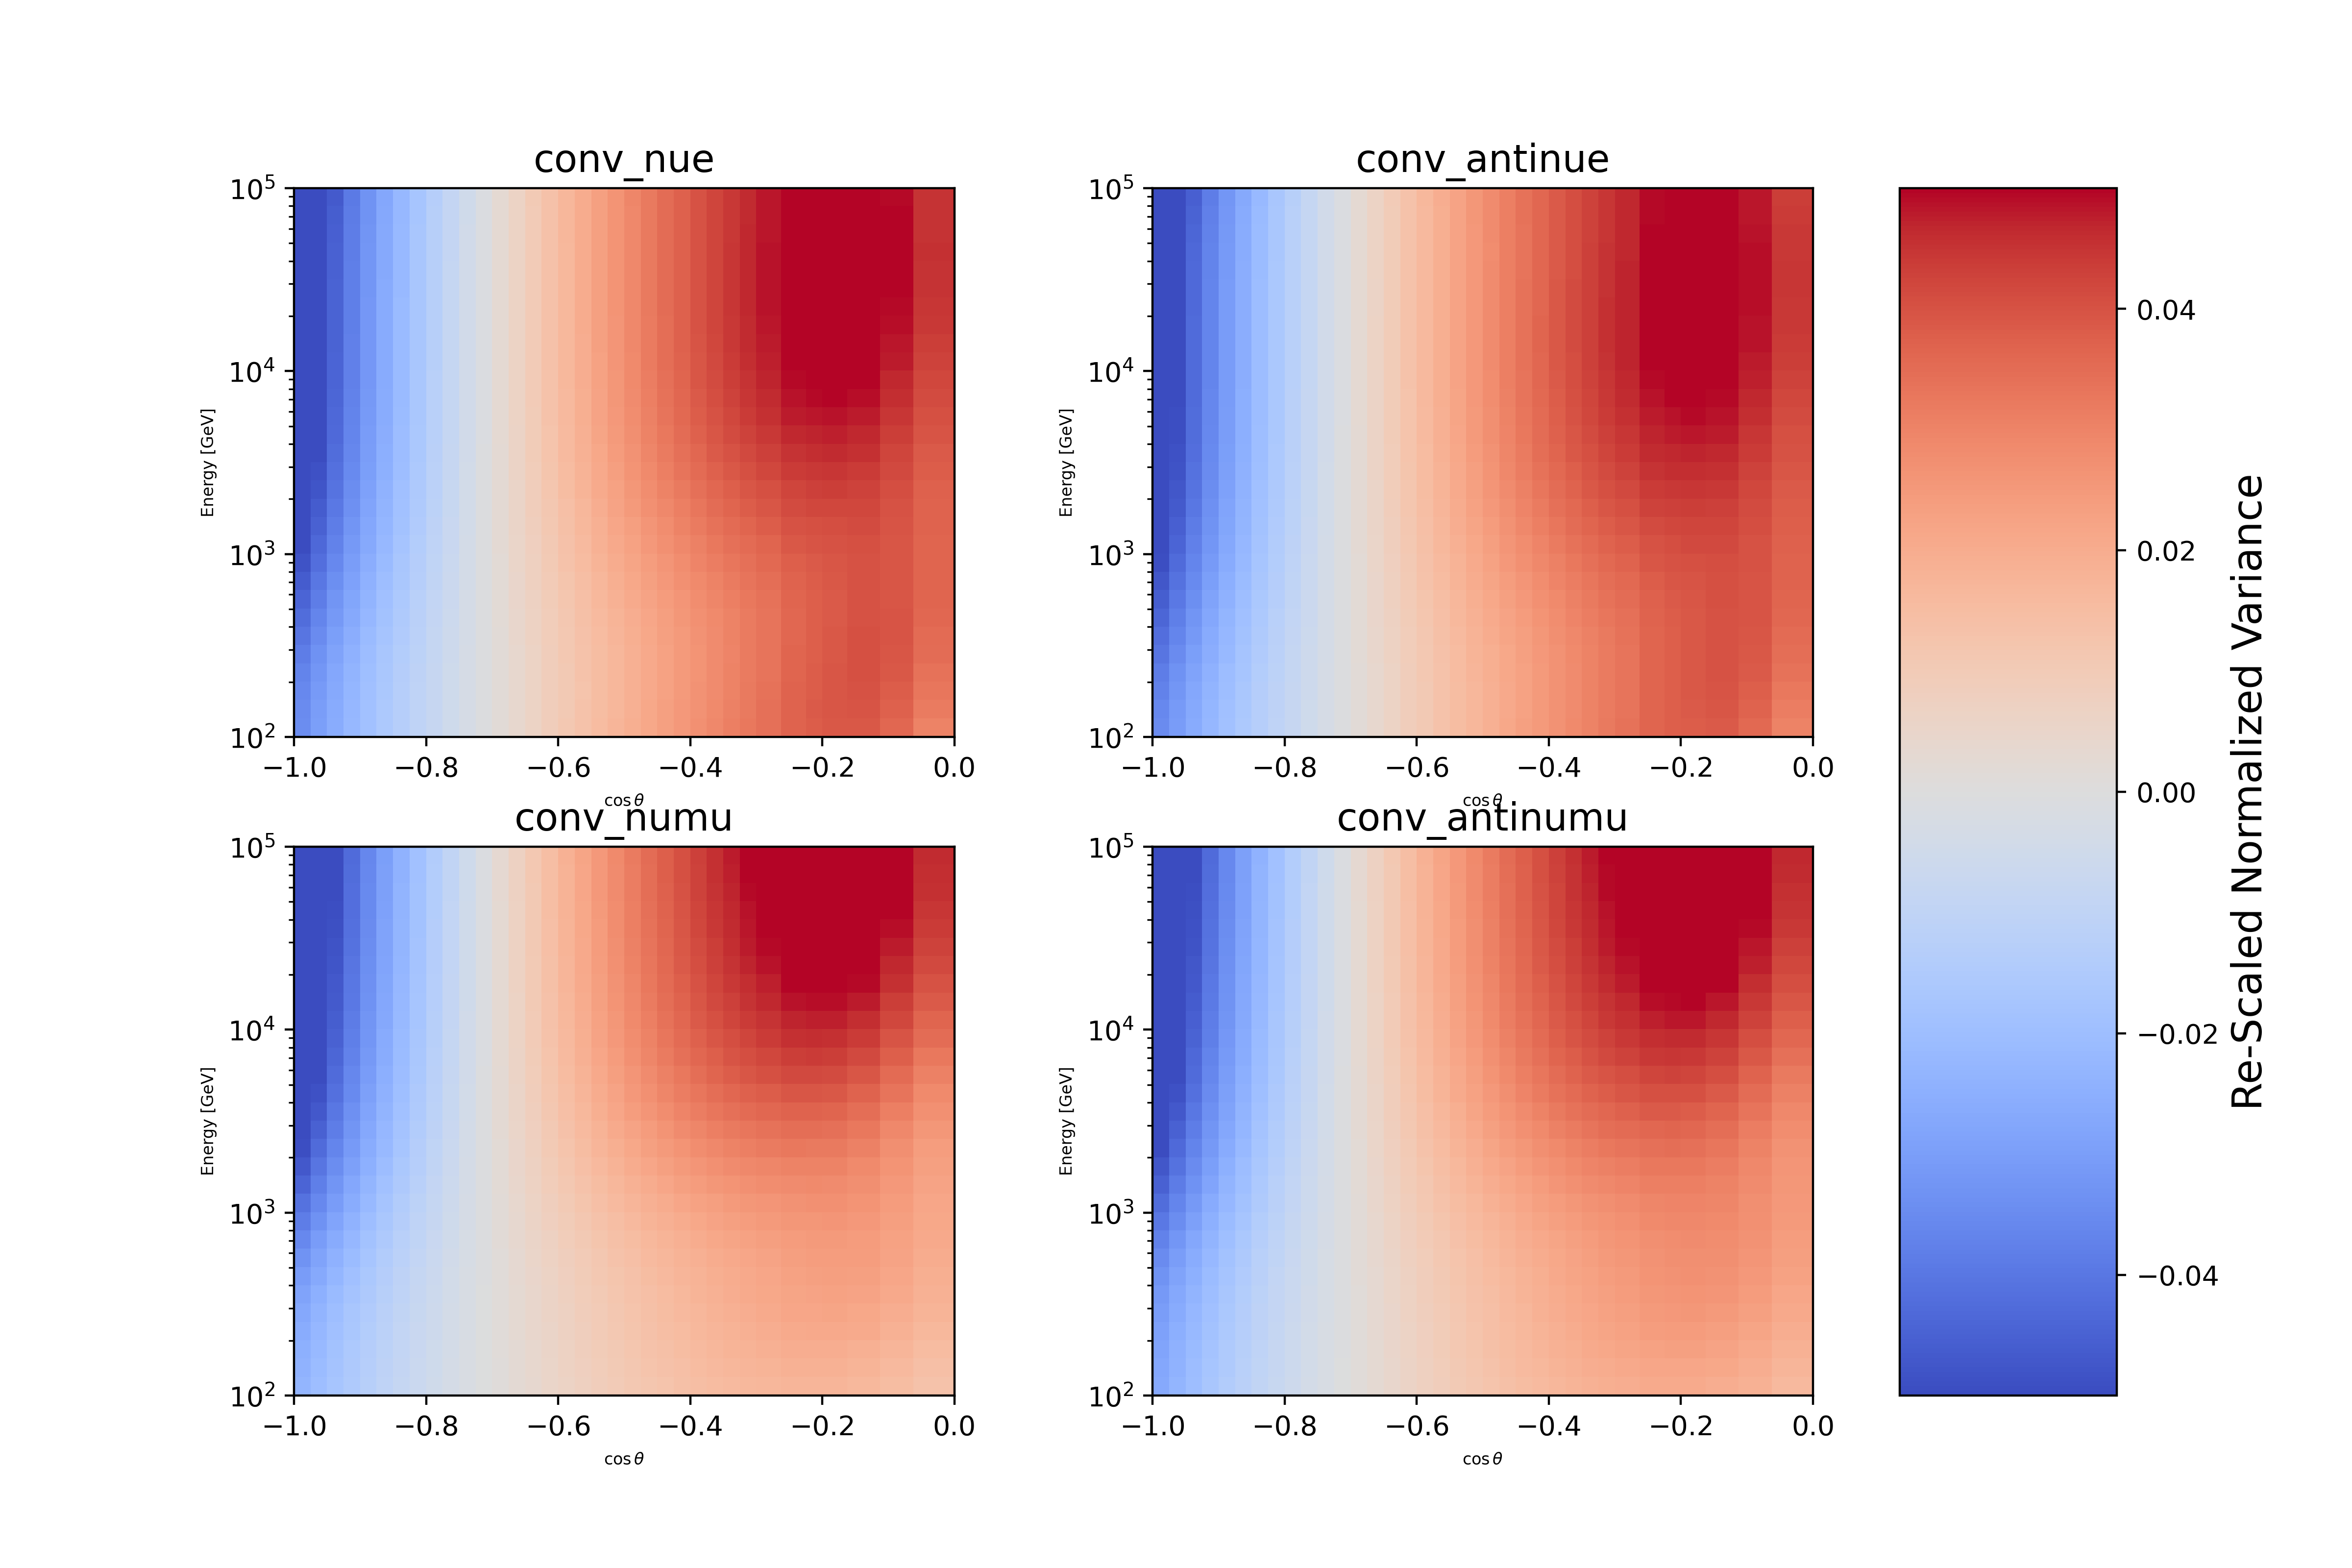
\includegraphics[width=0.8\linewidth]{figures/airs_grid.png}
    \caption{The effect of the atmospheric uncertainty parameter on predicted neutrino fluxes before nuSQuIDS propagation. This is after forcing the effect through zero at the equator, and implementing opposite effects in the opposite hemispheres. From the top left, going clockwise, $\nu_{e}$, $\bar{\nu}_{e}$, $\nu_{\mu}$, and $\bar{\nu}_{\mu}$.}\label{fig:airs_grid}
\end{figure}

\begin{figure}
    \centering
    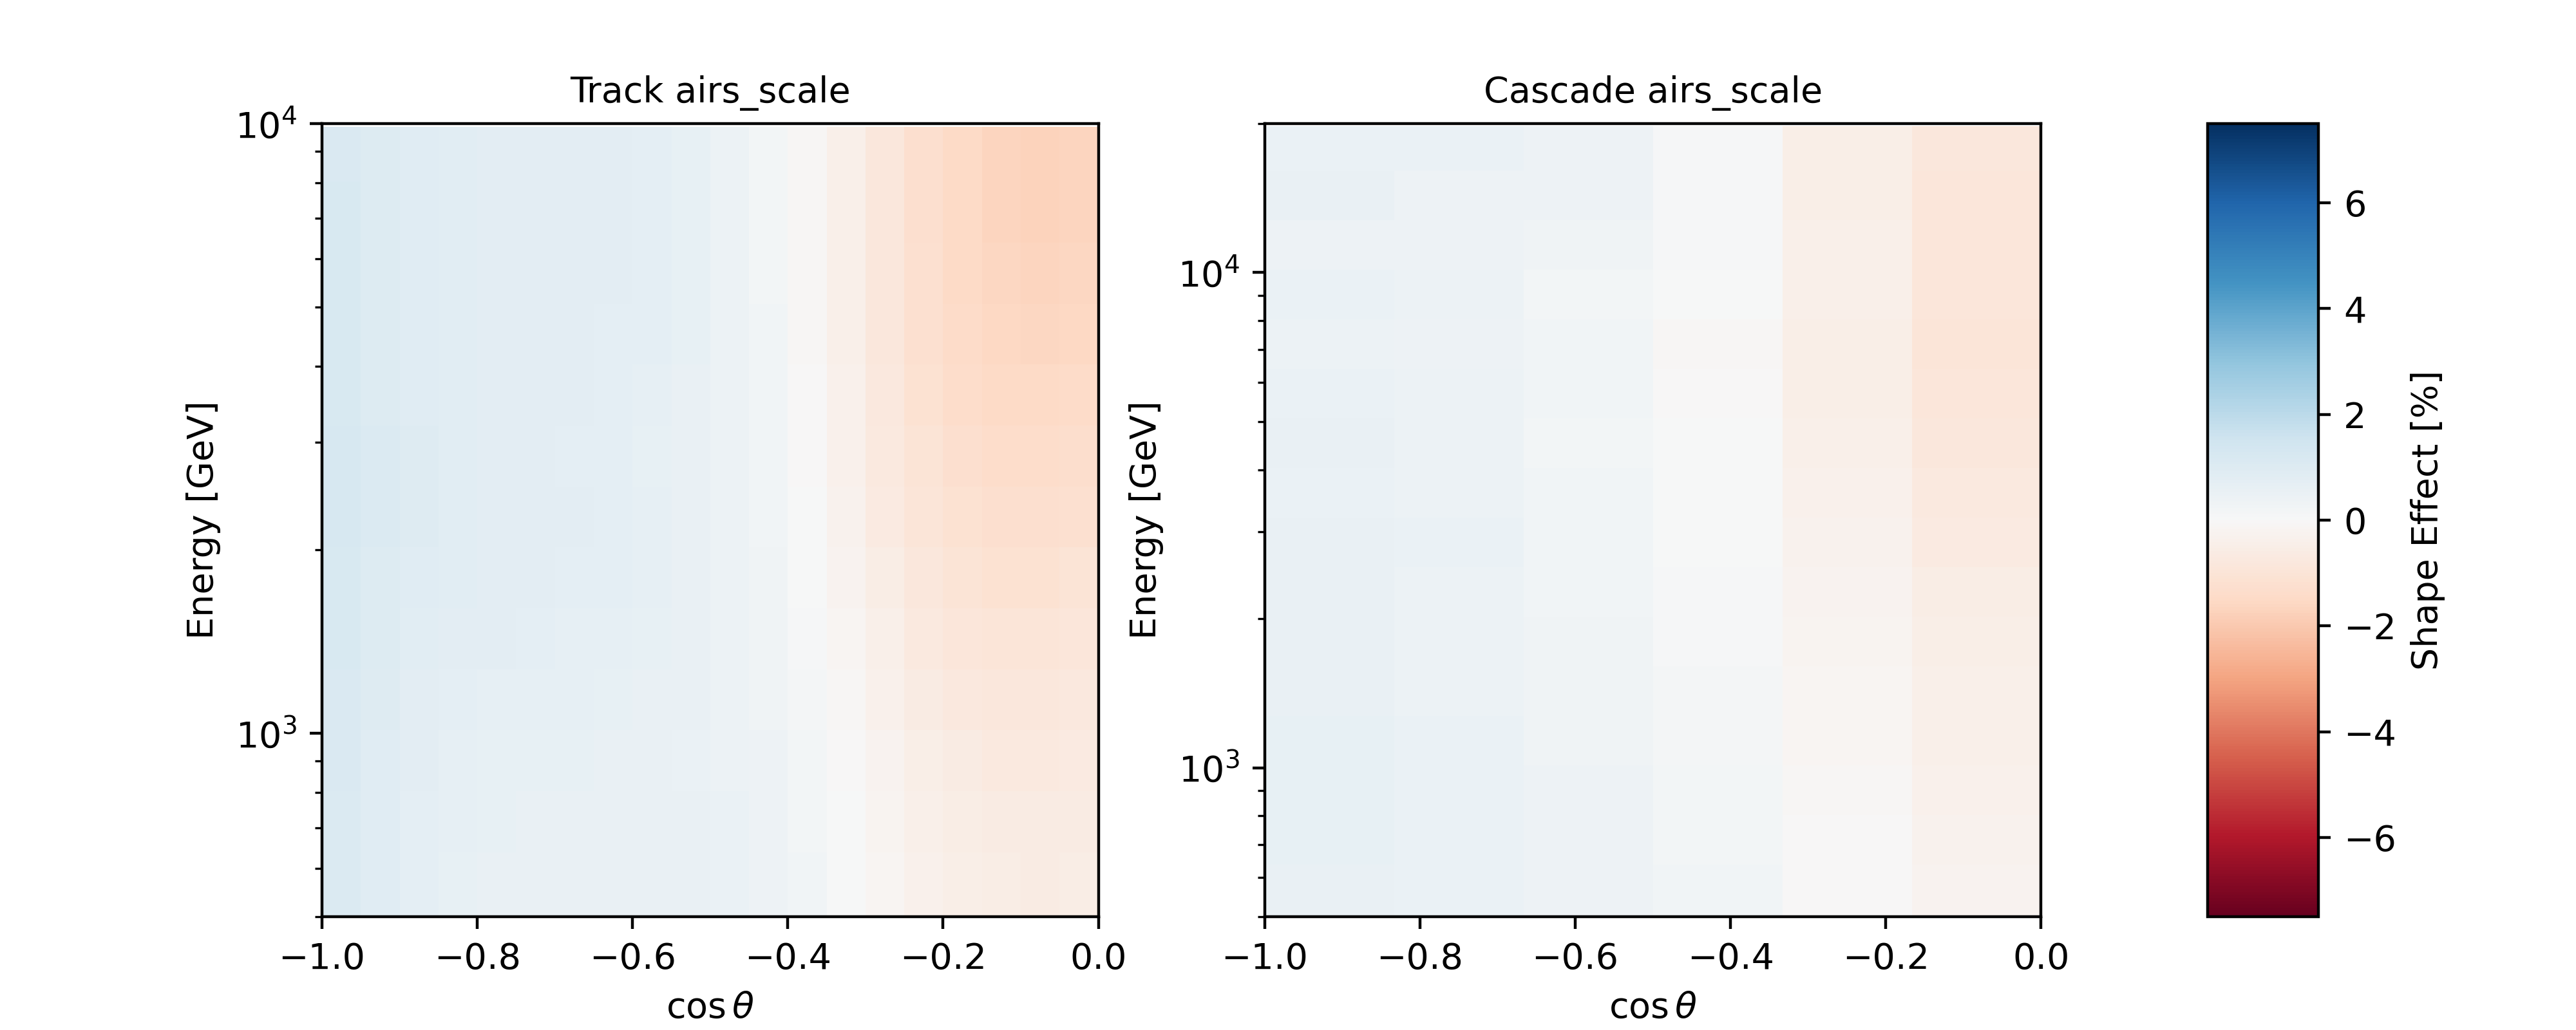
\includegraphics[width=0.8\linewidth]{figures/systematics/airs_scale.png}
    \caption{Effects of the atmospheric uncertainty on reconstructed event rates for tracks (left) and cascades (right).}\label{fig:airs_reco}
\end{figure}




\subsection{Kaon-nucleon Total Cross-Section}

The majority of the neutrino flux at the energies relevant to this analysis come from the decays of Kaons, as shown in Figure~\ref{fig:parentparty}.

\begin{figure}
    \centering
    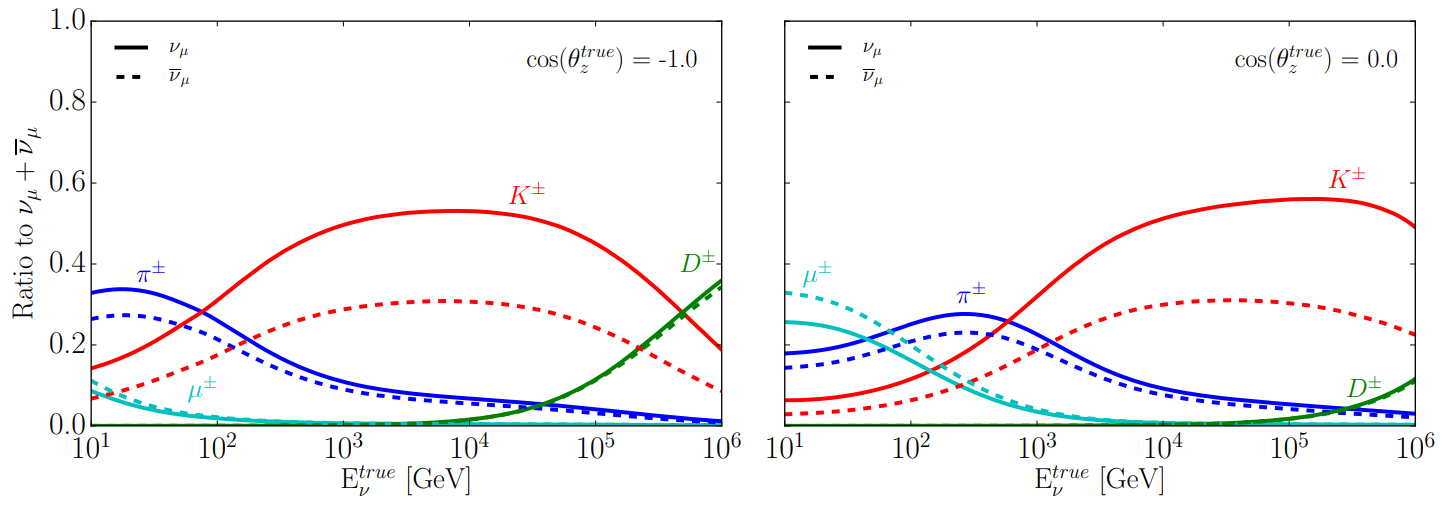
\includegraphics[width=0.8\linewidth]{./figures/parent_party.png}
    \caption{Contribution of different parent particles to the total atmospheric neutrino fluxes as functions of energy. The contributions to up-going neutrinos are shown on the left, and horizontal neutrinos are on the right. Figure from Ref~\cite{Aartsen_2020_prd}}\label{fig:parentparty}
\end{figure}

After the creation of a kaon it can either decay or inelastically scatter with the nucleons in the air. 
Such interactions would down-scatter the kaon to a lower energy in addition to creating other mesons. 
The relative probabilities of these can and do have a direct impact on the expected shape of the neutrino flux coming out of these cosmic ray air showers. 

Unfortunately, though, the total cross-section for $K^{\pm}$-nucleons has not been measured above the lower end of our energy spectrum, 310GeV~\cite{PhysRevD.98.030001}. 
Cross-section measurements have been done at higher energies using proton-proton collisions however, and one can extrapolate a kaon-nucleon cross-section through a Glauber~\cite{PhysRev.100.242, GLAUBER1970135} and Gribov-Regge~\cite{Gribov:1967vfb} multiple scattering formalism. 

A direct extrapolation of the uncertainty on the total kaon-nuclei cross-section of ~4\%, which we conservatively extrapolate out to a value of $\pm 7.5$\%. 
Future proton-Oxygen collisions in Run 3 at the LHC could constrain the uncertainty in this cross-section, however~\cite{Dembinski2020dam}.

\begin{figure}
    \centering
    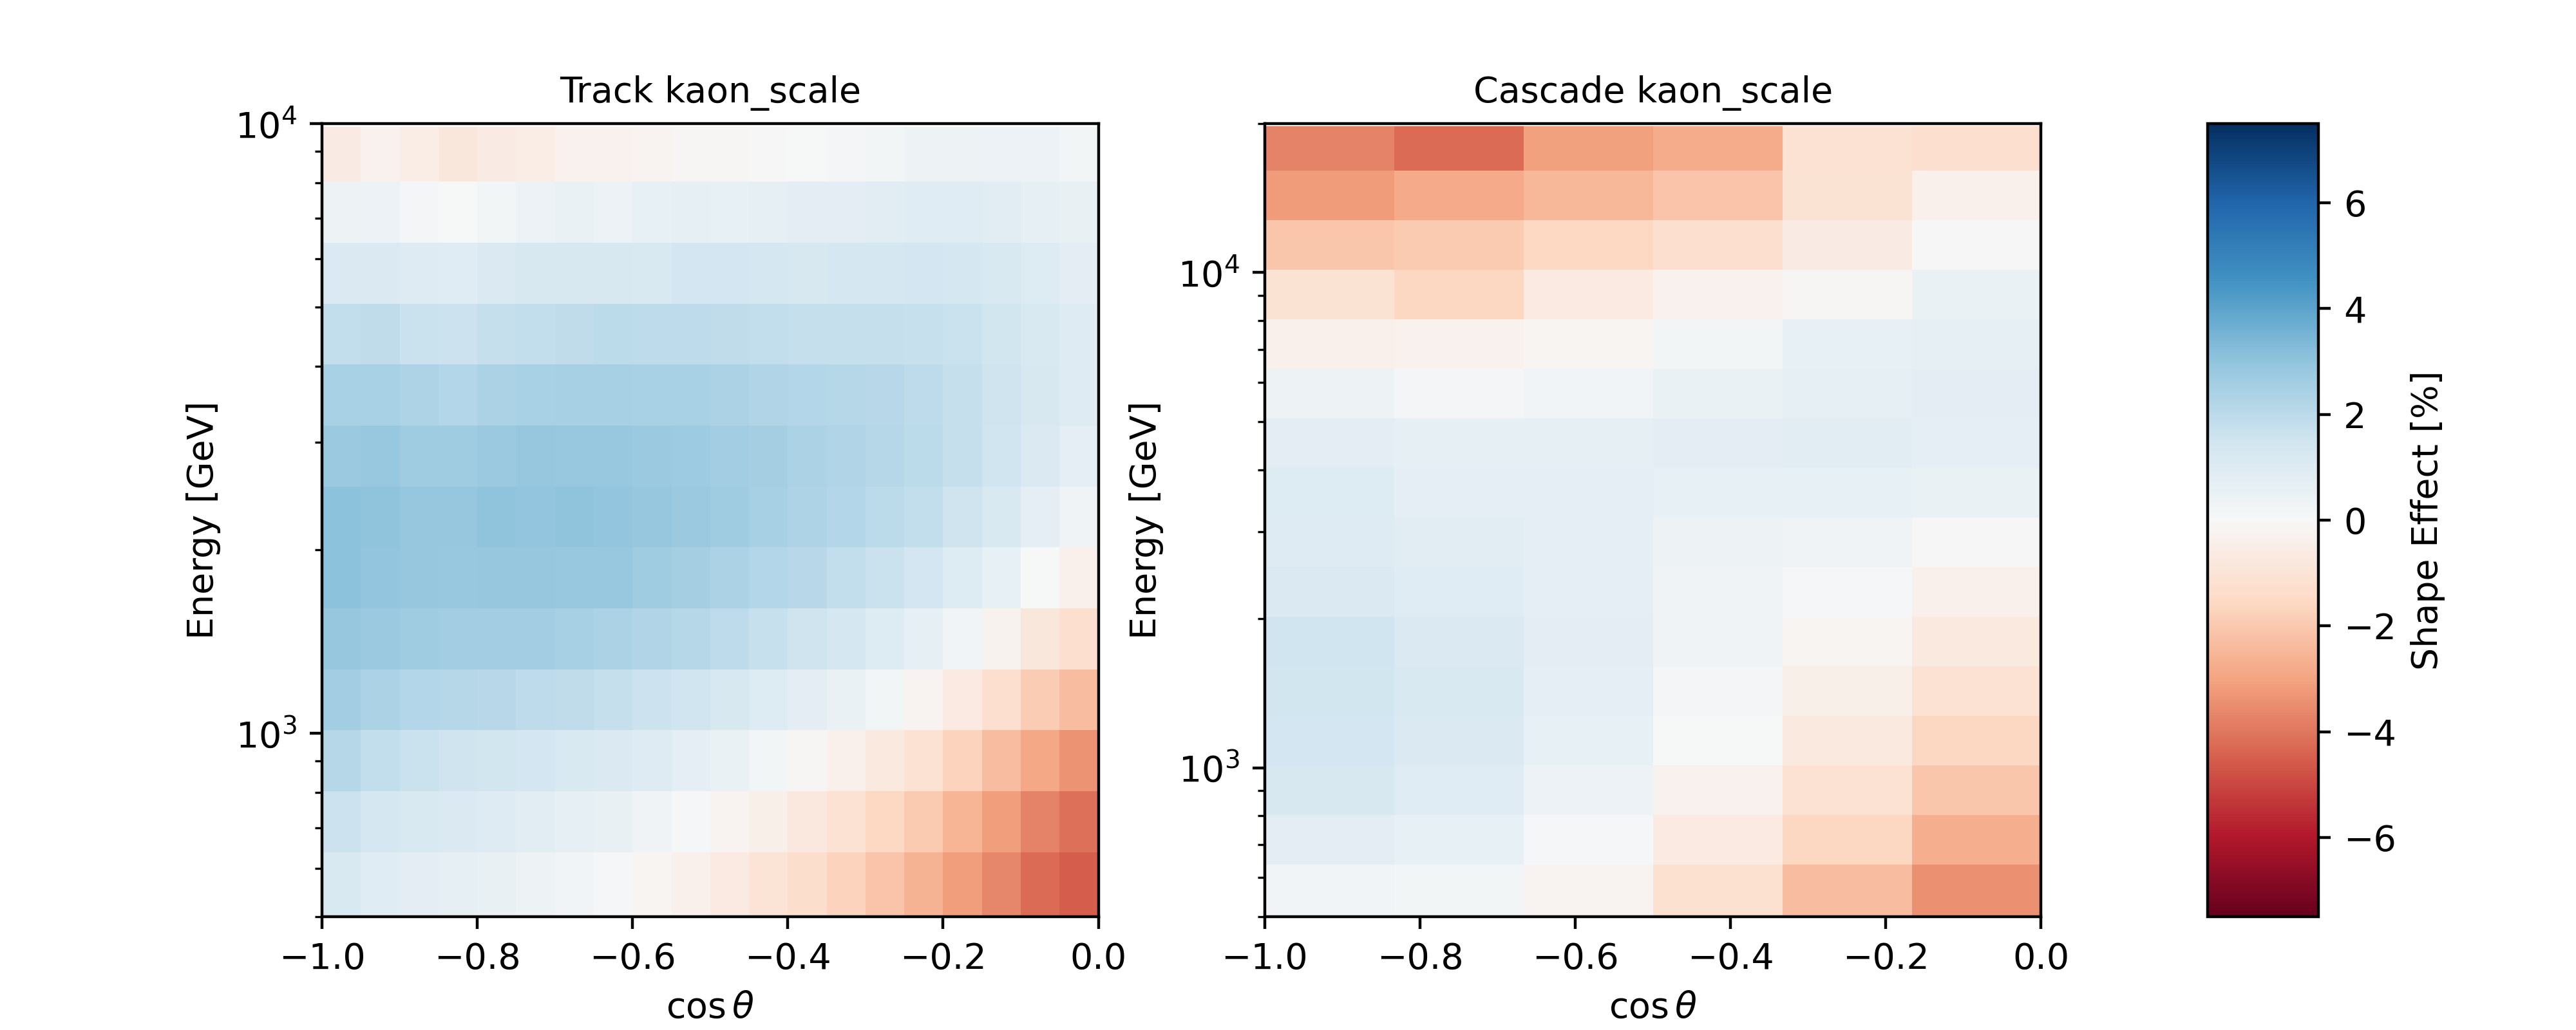
\includegraphics[width=0.8\linewidth]{figures/systematics/kaon_scale.png}
    \caption{The effects in analysis space on tracks (left) and cascades (right) after perturbing the kaon-nucleon cross-section by 7.5\%.}\label{fig:kaon}
\end{figure}

\subsection{Astrophysical Neutrino Flux}

Astrophysical neutrinos are a background to this analysis; it is modeled here as an isotropic, unbroken power law spectrum with equal contributions from each neutrino variety.
The priors are the same as for the previous track analyses~\cite{Aartsen_2020, Aartsen_2020_prd}, which use the IceCube High-Energy Starting Events sample~\cite{2021hese} to construct a correlated prior for the normalization and spectral index. 
Constraints are shown in Figure~\ref{fig:hese}, where the spectral index and normalization are defined according to 
\begin{equation}
    \dfrac{d N_{\nu}}{dE}  = \Phi_{astro}\left(\dfrac{E_{\nu}}{100\text{ TeV}}\right)^{-2.5 + \Delta_{\gamma_{\text{astro}}} }
\end{equation}
were $\Delta_{\gamma_{\text{astro}}}$ represents a shift in the spectral index, and the flux has a normalization $\Phi_{astro}$ at 100TeV of 
\begin{equation}
\Phi_{astro} = 0.787\times 10^{-18} \left[\text{GeV}\cdot\text{sr}\cdot\text{s}\cdot\text{cm}^{2}.\right]^{-1}
\end{equation}

\begin{figure}
    \centering
    \includegraphics[width=0.6\linewidth]{figures/hese.png}
    \caption{Constraints on the normalization and spectral index of the astrophysical neutrino flux. Contributions to the overall prior are shown from the Diffuse six-year sample CITE, the multi-year cascades sample, and from the HESE sample. Figure from Ref~\cite{Aartsen_2020_prd}.}\label{fig:hese}
\end{figure}

Two new uncorrelated nuisance parameters are constructed following the same procedures of Section~\ref{sect:down}. The effects of perturbing each of these new, uncorrelated, parameters are shown in Figure~\ref{fig:recoastro} with tracks on the left and cascades on the right.

\begin{figure}
    \centering
    \includegraphics[width=0.8\linewidth]{figures/systematics/astro_norm_rotated.png}\\
    \includegraphics[width=0.8\linewidth]{figures/systematics/astro_delta_rotated.png}
    \caption{Effects in analysis space for tracks (left) and cascades (right) from perturbing the uncorrelated astrophysical nuisance parameters (top and bottom) individually by one sigma. }\label{fig:recoastro}
\end{figure}

From Figure~\ref{fig:recoastro} it is evident that the astrophysical neutrinos contribute far more strongly to the cascade sample than to the tracks sample.
To demonstrate why this is the case, consider the fluxes and cross-sections contributing to each event morphology.

\begin{align}
    \text{Tracks} &\propto \Phi_{\nu_{\mu}}\times \sigma_{\nu_{\mu}}^{CC} \\
    \text{Cascades} &\propto \Phi_{\nu_{\mu}}\times \sigma_{\nu_{\mu}}^{NC}  + \sum_{\alpha\in (e,\tau)}\Phi_{\nu_{\alpha}}\times\left( \sigma_{\nu_{\alpha}}^{CC} +  \sigma_{\nu_{\alpha}}^{NC}\right)
\end{align}

For conventional fluxes, the electron and tau components are almost negligible. 
Whereas we can reasonably expect a 1-1-1 flavor ratio for the astrophysical neutrino flux. 
These contributions are demonstrated, to reasonable approximation, in Table~\ref{tab:astro_stuff}.
Since efficiencies are equivalent regardless of neutrino origin, these expressions are also consistent with total event rates. 
In the case of cascades, it is evident that the astrophysical neutrinos will contribute a proportionally greater amount to the total event rate. 


\begin{table}
    \centering
    \renewcommand{\arraystretch}{1.2}
    \rowcolors{2}{gray!25}{white}
    \begin{tabular}{c|c|c}\rowcolor{blue!25}
        & \textbf{Tracks} & \textbf{Cascades} \\
    \textbf{Conv} & $ \Phi_{\nu_{\mu}}^{conv}\times \sigma_{\nu_{\mu}}^{CC}$ & $\Phi_{\nu_{\mu}}^{conv}\times \sigma_{\nu_{\mu}}^{NC}$ \\[10pt]
    \textbf{Astro}    & $\Phi_{\nu_{\mu}}^{astr}\times \sigma_{\nu_{\mu}}^{CC}$ & $\Phi_{\nu_{\mu}}^{astro}\times \sigma_{\nu_{\mu}}^{NC}  + \sum\limits_{\alpha\in (e,\tau)}\Phi_{\nu_{\alpha}}^{astro}\times\left( \sigma_{\nu_{\alpha}}^{CC} +  \sigma_{\nu_{\alpha}}^{NC}\right)$
    \end{tabular}
    \caption{Taaaaable words}\label{tab:astro_stuff}
\end{table}



\subsection{Neutrino-Nucleon Interaction Uncertainty}
\index{neutrino!cross section}
\index{neutrino!interactions}
Neutrino-nucleon cross-sections, in the context of this high-energy work, are well beyond the `even remotely' regime of MeV, or even few-GeV, analyses.
We are well and truly under the rule of the DIS kingdom. 
The cross-section at these energies runs in energy as a power law with a knee near $10^{4}$ GeV as valence quark interaction parton density begins to weaken compared to the sea~\cite{GANDHI199681}.

While the uncertainty was previously found to be inconsequential to the event rate at the detector~\cite{osti_1221354, 2015PhDT94D}, it also manifests as the degree to which high-energy neutrino fluxes are attenuated as they propagate through the Earth ~\cite{Vincent:2017svp, PhysRevD.83.113009, Cooper_Sarkar_2011}. 
Although previous analyses for tracks had found this to be a not-negligible source of uncertainty~\cite{Aartsen_2020, Aartsen_2020_prd}, this was not the case for the cascades sample where the reconstructed cascade energy is closer to the true energy of the parent neutrino.
The effects of the uncertainties on the neutrino and antineutrino cross-section on reconstructed cascade event rate are shown in Figure~\ref{fig:nucross}.
Because the effects are so small, we elected to fix the uncertainty of the neutrino-nucleon cross-section to its central value in fits. 

\begin{figure}
    \centering
    \includegraphics[width=0.7\linewidth]{figures/systematics/nu_scale.png} \\
    \includegraphics[width=0.7\linewidth]{figures/systematics/nubar_scale.png}
    \caption{The effects of neutrino (antineutrino) cross-section uncertainty are shown on the top (bottom) for tracks (left) and cascades (right). Effect manifests as a sub-percent level disappearance of Earth-crossing events at energies over 10TeV.}\label{fig:nucross}
\end{figure}


\subsection{Cosmic Ray Muon Background}

One of the most difficult sources of background in IceCube comes from the muons forged in the cosmic ray air showers above IceCube. 
These muons enter IceCube at a rate of about 2 kilohertz, and so over the ten years of livetime for the cascades sample, an estimated $3.15\times 10^{11}$ muons would have entered the volume over a wide range of energies. 
Although the series of filters are highly effective at cutting these sneaking muons, several still manage to enter in and deposit light near the center of IceCube, and pass the event selection criteria. 
The numbers of cosmogenic muons which pass these cuts, and are misidentified as neutrino cascades, and the percent of each bin they encompass, is shown in Figure~\ref{fig:muonperc}.

\begin{figure}
    \centering
    \includegraphics[width=0.8\linewidth]{figures/expectation_stacked.png}
    \caption{A stacked histogram showing the contributions,  to the total event counts as a function of reconstructed energy, from conventional neutrinos (orange), prompt neutrinos (salmon), astrophysical neutrinos (purple), and cosmic ray muons misidentified as cascades (deeper purple). The percent of each bin which is made of CR muons is show as a black dashed line.}\label{fig:muonperc}
\end{figure}

The distribution of these muon events in reconstructed energy and zenith is shown in Figure~\ref{fig:muonmuon}, left.
Due to the large number of events necessary to simulate to recover MC-statistically significant muon rates, a Gaussian kernel density estimate (KDE) is used to approximate the expected distribution that would likely lead to the simulated MC sample. 
The expected distribution of events is shown after the KDE smoothing is applied in Figure~\ref{fig:muonmuon}, right. 

\begin{figure}
    \centering
    \includegraphics[width=0.45\linewidth]{figures/muons_nokde.png}%
    \includegraphics[width=0.45\linewidth]{figures/kde_muons.png}
    \caption{2D heatmaps showing the expected number of muons after ten years of livetime in the analysis binning. Rates are shown before (left) and after (right) the kernel density smoothing is applied.}\label{fig:muonmuon}
\end{figure}

Uncertainty on these muons is extrapolated from the original MC statistical error. 
The same KDE smoothing procedure is carried out on the sum of the squares of the weights in each bin; the resulting error and the ratio between the error and means are shown in Figure~\ref{fig:muonmuonerr}

\begin{figure}
    \centering
    \includegraphics[width=0.45\linewidth]{figures/kde_muons_error.png}%
    \includegraphics[width=0.45\linewidth]{figures/kde_muons_error_ratio.png}
    \caption{2D heatmaps showing the KDE-smoothed MC statistical error for the muons (left) and the ratio of this value to the mean calculated from the KDE-smoothed muon rates (right).}\label{fig:muonmuonerr}
\end{figure}

The overall normalization of the muon rate is allowed to float freely in fits with a 20\% prior width chosen to match that of the neutrino fluxes, and the per-bin error on the muons is considered large enough to account for the variance possible from MC statistical error.
The shape effect from allowing the atmospheric muon scale to float is shown in Figure~\ref{fig:muon_shape}.

\begin{figure}
    \centering
    \includegraphics[width=0.8\linewidth]{figures/atm_muon_scale.png}
    \caption{The shape-only effect of increasing the CR muon normalization by 20\%. This manifests as an increase in event rates at 1-3 TeV across all zeniths; apparent suppression at high energies is an artifact of this being a shape-only plot.}\label{fig:muon_shape}
\end{figure}

The possibility of using a set of cuts was investigated as well. 
Multiple additional reconstructed quantities are available to us, beyond just energy and zenith, with which cuts can be applied. 
The track and cascade boosted decision-tree scores, reconstructed depth, and the reconstructed `contained-ness' of the events all provide extra leverage with which cosmic ray muons and true neutrino events can be discriminated.
A series of cuts, listed in Table~\ref{tab:cut_table}, were found capable of cutting all simulated CR muons out of the cascades sample.
The required cuts were found to be so aggressive that the remaining signal neutrinos would be insufficient to have enough statistics to allow for studying the sterile neutrino signal.
The number of events, before (left) and after (right) the extra set of cuts were applied, is shown in Figure~\ref{fig:cut_figure}.
Only 13\% of the original neutrino sample passed all cuts. 
Because of this, these extra cuts are not applied in this analysis. 

\begin{table}
    \centering
    \rowcolors{2}{gray!25}{white}
    \begin{tabular}{c|cc}\rowcolor{blue!25}
        Parameter & Minimum & Maximum \\\hline
        $\cos\theta_{reco}$ & -1.0 & 0.0 \\
        $z_{reco}$ & n/a & -300 \\
        BDT-Track & n/a & 0.02 \\
        BDT-Cascade & 0.2 & 0.75
    \end{tabular}
    \caption{A series of cuts capable of removing all of the CR muon background.}\label{tab:cut_table}
\end{table}


\begin{figure}
    \centering
    \includegraphics[width=0.45\linewidth]{figures/zenith_only_cut.png}%
    \includegraphics[width=0.45\linewidth]{figures/all_cuts.png}
    \caption{The number of events over the full 10 years of livetime showing the contributions to the total event rate from all even populations. On the left, only a cut on the reconstructed zenith is applied such that $\cos\theta_{reco}<0$. On the right, the full set of cuts listed in Table~\ref{tab:cut_table} is applied. }\label{fig:cut_figure}
\end{figure}

\subsection{Normalization}

A parameter allowing for the overall normalization of the entire neutrino flux is also allowed to float. It is given a conservative 20\% prior driven by a number of effects: livetime O(<1\%), ice density O(<1\%), volume O(9\%)~\cite{Sandrock_2020}, and the neutrino-ice cross-section O(10\%)~\cite{candido2023neutrino}.

\subsection{All Systematic Uncertainties}

A table showing parameterizations of all included systematic uncertainties, their central values, and the prior widths, are included in Table~\ref{table:nutrition}.

\begin{table}
    \centering
    \rowcolors{2}{gray!25}{white}
    \begin{tabular}{c | cccc}\rowcolor{blue!25}
        {\large \textbf{Parameter}} & {\large \textbf{Center}} & {\large \textbf{Prior}} & {\large \textbf{Boundary}}& {\large \textbf{Morphology}} \\ \hline
        \multicolumn{5}{c}{Conventional Flux} \\\hline
        Atm. Density & 0.0 & 0.0$\pm$1.0 & [-4.0, 4.0] & Both\\
        Kaon energy loss $\sigma_{KA}$ & 0.0 & $0.0\pm1.0$ & [-4.0, 4.0]& Both \\
        daemon\_0$^{*}$  & 0.0 & $0.0\pm1.0$ & [-4, 4]& Both\\
        daemon\_1$^{*}$  & 0.0 & $0.0\pm1.0$ & [-4, 4]& Both\\
        daemon\_9$^{*}$  & 0.0 & $0.0\pm1.0$ & [-4, 4]& Both\\
        daemon\_12$^{*}$  & 0.0 & $0.0\pm1.0$ & [-4, 4]& Both\\
        daemon\_18$^{*}$ & 0.0 & $0.0\pm1.0$ & [-4, 4]& Both\\
        daemon\_19$^{*}$ & 0.0 & $0.0\pm1.0$ & [-4, 4]& Both\\
        daemon\_20$^{*}$ & 0.0 & $0.0\pm1.0$ & [-4, 4]& Both\\
        daemon\_23$^{*}$ & 0.0 & $0.0\pm1.0$ & [-4, 4]& Both\\
        \multicolumn{5}{c}{Astrophysical Flux} \\\hline
        astro\_rotated\_0$^{\dag}$ & 0.0 & $0.0\pm 0.42 $ & [-2.1, 2.1]&Both\\
        astro\_rotated\_1$^{\dag}$ & 0.0 & $0.0\pm0.20$ & [-0.95, 0.95]&Both\\
        \multicolumn{5}{c}{Detector} \\\hline
        hole\_ice\_scale & -1.0 & $-1\pm10$ & [-4, 1]&Tracks \\
        holeice p$_{0}$ & 0.0 & $0\pm 1.0$ & [-4,4]&Cascades\\
        holeice p$_{1}$ & 0.0 & $0\pm 1.0$ & [-4,4]&Cascades\\
        ice\_0$^{\ddag}$ & 0.0 & $0\pm 1.0$ & [-4,4]&Cascades\\
        ice\_1$^{\ddag}$ & 0.0 & $0\pm 1.0$ & [-4,4]&Cascades\\
        ice\_4$^{\ddag}$ & 0.0 & $0\pm 1.0$ & [-4,4]&Cascades\\
        ice\_6$^{\ddag}$ & 0.0 & $0\pm 1.0$ & [-4,4]&Cascades\\
        ice\_grad\_0\_rotated$^{**}$ & 0.0 & $0\pm 1.0$ & [-4,4] & Tracks\\
        ice\_grad\_0\_rotated$^{**}$ & 0.0 & $0\pm 1.0$ & [-4,4]& Tracks \\
        DOM Efficiency & 1.0 & $1.00\pm0.123$ & [0.972, 1.058] & Both \\
        \multicolumn{5}{c}{Muons} \\\hline
        muon norm & 1.0 & $1.0\pm0.2$ & [0,2] & Cascades\\
        \multicolumn{5}{c}{Normalization} \\\hline
        norm & 1.0 & $1.0\pm0.2$ & [0,2] & Both
    \end{tabular}
    \caption{The central values, priors, and boundaries for all nuisance parameters. The ice gradients, Daemonflux, and astrophysical parameters are all listed here in the uncorrelated basis and in terms of the $1\sigma$ widths determined from a PCA of their covariance matrices; these parameters are linear combinations of correlated parameters and are marked with $*$,$**$ $\dag$, or $\ddag$.}\label{table:nutrition}
\end{table}

\end{document}